% \documentclass[a4paper,10pt]{article} % or whatever
% \documentclass[letterpaper,10pt]{article} % or whatever
\documentclass{article}

% if you need to pass options to natbib, use, e.g.:
     \PassOptionsToPackage{numbers, compress}{natbib}

\usepackage[preprint]{notes}
\usepackage{soul}

\newcommand{\ignore}[1]{}
% to avoid loading the natbib package, add option nonatbib:
\usepackage{dsfont}

% Note: this has been tested using MiKTeX 2.9. If you are getting errors, update your packages.

%%% Packages %%%
%\usepackage{setspace} % Double spaces document. Footnotes,
                      % figures, and tables will still be single spaced, however.
%\doublespacing
%\singlespacing
%\onehalfspacing
% \setstretch{1.5} % set double spacing to 1.5 or anything else.

\usepackage[T1]{fontenc}
\usepackage{amsmath,amssymb,amsfonts,mathrsfs,bm}% Typical maths resource packages
\usepackage{mathtools}
%\let\proof\relax
%\let\endproof\relax
\usepackage{amsthm}
\usepackage{nicefrac}
%\usepackage{cite}
%\let\labelindent\relax
\usepackage[shortlabels]{enumitem}
\usepackage{graphicx}
\usepackage{epstopdf}
\usepackage{url}
\usepackage{colortbl}
\usepackage{booktabs}
\usepackage{multirow}
\usepackage[table,dvipsnames]{xcolor}
\usepackage[normalem]{ulem}
\usepackage{xparse}

%\usepackage{pstricks}
%\usepackage{psfrag}
%\usepackage{syntonly}
%\syntaxonly
%\usepackage[style=base]{caption}
%\captionsetup{
    %format = plain,
    %font = footnotesize,
    %labelfont = sc
%}


\usepackage{array}
\newcolumntype{L}[1]{>{\raggedright\let\newline\\\arraybackslash\hspace{0pt}}m{#1}}
\newcolumntype{C}[1]{>{\centering\let\newline\\\arraybackslash\hspace{0pt}}m{#1}}
\newcolumntype{R}[1]{>{\raggedleft\let\newline\\\arraybackslash\hspace{0pt}}m{#1}}

\makeatletter
\let\MYcaption\@makecaption
\makeatother
\usepackage[font=footnotesize]{subcaption}
\makeatletter
\let\@makecaption\MYcaption
\makeatother


% achieves the functionality of \tag for subequations environment
\makeatletter
\newenvironment{varsubequations}[1]
 {%
  \addtocounter{equation}{-1}%
  \begin{subequations}
  \renewcommand{\theparentequation}{#1}%
  \def\@currentlabel{#1}%
 }
 {%
  \end{subequations}\ignorespacesafterend
 }
\makeatother


\usepackage{glossaries}

\makeatletter
% copy old \gls and \glspl
\let\oldgls\gls
\let\oldglspl\glspl

% define a non space skipping version of \@ifnextchar
\newcommand\fussy@ifnextchar[3]{%
  \let\reserved@d=#1%
  \def\reserved@a{#2}%
  \def\reserved@b{#3}%
  \futurelet\@let@token\fussy@ifnch}
\def\fussy@ifnch{%
  \ifx\@let@token\reserved@d
    \let\reserved@c\reserved@a 
  \else
    \let\reserved@c\reserved@b
  \fi
 \reserved@c}

\renewcommand{\gls}[1]{%
  \oldgls{#1}\fussy@ifnextchar.{\@checkperiod}{\@}}
\renewcommand{\glspl}[1]{%
  \oldglspl{#1}\fussy@ifnextchar.{\@checkperiod}{\@}}

\newcommand{\@checkperiod}[1]{%
  \ifnum\sfcode`\.=\spacefactor\else#1\fi
}
\makeatother

%%%%%%%%%%%%% new add %%%%%%%%%%%%% 
\newcommand{\tb}[1]{\textbf{#1}}


\newacronym{wrt}{w.r.t.}{with respect to}
\newacronym{RHS}{R.H.S.}{right-hand side}
\newacronym{LHS}{L.H.S.}{left-hand side}
\newacronym{iid}{i.i.d.}{independent and identically distributed}
%\newacronym{MIMO}{MIMO}{mulitple-input multiple-output}
%\newacronym{AOA}{AOA}{angle-of-arrival}
%\newacronym{AOD}{AOD}{angle-of-departure}
%\newacronym{LOS}{LOS}{line-of-sight}
%\newacronym{NLOS}{NLOS}{non-line-of-sight}
%\newacronym{TOA}{TOA}{time-of-arrival}
%\newacronym{TDOA}{TDOA}{time-difference-of-arrival}
%\newacronym{RSS}{RSS}{received signal strength}
%\newacronym{GNSS}{GNSS}{Global Navigation Satellite System}
%\newacronym{GSP}{GSP}{graph signal processing}
%\newacronym{ML}{ML}{machine learning}


%put the float package before hyperref and algorithm package after hyperref for hyperref to work correctly with algorithm
\usepackage{float}

\ifx\notloadhyperref\undefined
	\ifx\loadbibentry\undefined
		\usepackage[hidelinks,hypertexnames=false]{hyperref} 
	\else
		\usepackage{bibentry}
		\makeatletter\let\saved@bibitem\@bibitem\makeatother
		\usepackage[hidelinks,hypertexnames=false]{hyperref}
		\makeatletter\let\@bibitem\saved@bibitem\makeatother
	\fi
\else
	\ifx\loadbibentry\undefined
		\relax
	\else
		\usepackage{bibentry}
	\fi
\fi

\usepackage[capitalize]{cleveref}
\crefname{equation}{}{}
\Crefname{equation}{}{}
\crefname{claim}{claim}{claims}
\crefname{step}{step}{steps}
\crefname{line}{line}{lines}
\crefname{condition}{condition}{conditions}
\crefname{dmath}{}{}
\crefname{dseries}{}{}
\crefname{dgroup}{}{}

\crefname{Problem}{Problem}{Problems}
\crefformat{Problem}{Problem~(#2#1#3)}
\crefrangeformat{Problem}{Problems~(#3#1#4) to~(#5#2#6)}

\crefname{Theorem}{Theorem}{Theorems}
\crefname{Corollary}{Corollary}{Corollaries}
\crefname{Proposition}{Proposition}{Propositions}
\crefname{Lemma}{Lemma}{Lemmas}
\crefname{Definition}{Definition}{Definitions}
\crefname{Example}{Example}{Examples}
\crefname{Assumption}{Assumption}{Assumptions}
\crefname{Remark}{Remark}{Remarks}
\crefname{Rem}{Remark}{Remarks}
\crefname{remarks}{Remarks}{Remarks}
\crefname{Appendix}{Appendix}{Appendices}
\crefname{Supplement}{Supplement}{Supplements}
\crefname{Exercise}{Exercise}{Exercises}
\crefname{Theorem_A}{Theorem}{Theorems}
\crefname{Corollary_A}{Corollary}{Corollaries}
\crefname{Proposition_A}{Proposition}{Propositions}
\crefname{Lemma_A}{Lemma}{Lemmas}
\crefname{Definition_A}{Definition}{Definitions}
\crefname{rema}{Remark}{Remarks}
\crefname{exma}{Example}{Examples}

\usepackage{crossreftools}
\ifx\notloadhyperref\undefined
	\pdfstringdefDisableCommands{%
			\let\Cref\crtCref
			\let\cref\crtcref
	}
\else
	\relax
\fi

\usepackage{algorithm,algorithmic}
\renewcommand{\algorithmicrequire}{\textbf{Input:}}
\renewcommand{\algorithmicensure}{\textbf{Output:}}

%may cause conflict with some packages like tikz, include manually if desired
%load after hyperref
\ifx\loadbreqn\undefined
	\relax
\else
	\usepackage{breqn} 
\fi



%%%%%%%%%%%%%%%%%%%%%%%%%%%%%%%%%%%%%%%%%%%%%%%%


\interdisplaylinepenalty=2500   % To restore IEEEtran ability to automatically break
                                % within multiline equations, when using amsmath.

%%%%%%%%%%%%%%%%%%%%%%%%%%%%%%%%%%%%%%%%

%Theorem declarations

\ifx\renewtheorem\undefined
% for use in main body
\ifx\useTheoremCounter\undefined
\newtheorem{Theorem}{Theorem}
\newtheorem{Corollary}{Corollary}
\newtheorem{Proposition}{Proposition}
\newtheorem{Lemma}{Lemma}
\else
\newtheorem{Theorem}{Theorem}
\newtheorem{Corollary}[theorem]{Corollary}
\newtheorem{Proposition}[theorem]{Proposition}
\fi

\newtheorem{Definition}{Definition}
\newtheorem{Example}{Example}
\newtheorem{Remark}{Remark}
\newtheorem{Assumption}{Assumption}
\newtheorem{Exercise}{Exercise}

% for use in the appendix
\newtheorem{Theorem_A}{Theorem}[section]
\newtheorem{Corollary_A}{Corollary}[section]
\newtheorem{Proposition_A}{Proposition}[section]
\newtheorem{Lemma_A}{Lemma}[section]
\newtheorem{Definition_A}{Definition}[section]
\fi

\usepackage{amsmath}
\numberwithin{equation}{section} % or whatever you prefer
% \swapnumbers % I prefer this
% \theoremstyle{plain}
\newtheorem{thma}[equation]{Theorem}
\newtheorem{propa}[equation]{Proposition}
\newtheorem{lema}[equation]{Lemma}
\newtheorem{defa}[equation]{Definition}
\newtheorem{cora}[equation]{Corollary}
\newtheorem{Lemma_AA}{Lemma}[section]
\newtheorem{rema}[equation]{Remark}
\newtheorem{exma}[equation]{Example}
\newcommand{\ml}[1]{\begin{multlined}#1\end{multlined}}
\newcommand{\nn}{\nonumber\\ }


% Remarks
\theoremstyle{remark}
\newtheorem{Rem}{Remark}
\theoremstyle{plain}

\newenvironment{remarks}{
	\begin{list}{\textit{Remark} \arabic{Rem}:~}{
    \setcounter{enumi}{\value{Rem}}
    \usecounter{Rem}
    \setcounter{Rem}{\value{enumi}}
    \setlength\labelwidth{0in}
    \setlength\labelsep{0in}
    \setlength\leftmargin{0in}
    \setlength\listparindent{0in}
    \setlength\itemindent{15pt}
		}
}{
	\end{list}
}


% Special Headings
%\newtheorem*{Prop1}{Proposition 1} %needs amsthm

%\newtheoremstyle{nonum}{}{}{\itshape}{}{\bfseries}{.}{ }{#1 (\mdseries #3)}
%\theoremstyle{nonum}
%\newtheorem{Example**}{Example 1}

\newcommand{\EndExample}{{$\square$}}
%\renewcommand{\QED}{\QEDopen} % changes end of proof box to open box.

\newcommand{\qednew}{\nobreak \ifvmode \relax \else
      \ifdim\lastskip<1.5em \hskip-\lastskip
      \hskip1.5em plus0em minus0.5em \fi \nobreak
      \vrule height0.75em width0.5em depth0.25em\fi}


%\newcommand{\em}[1]{\emph{#1}}

% Move down subscripts for some symbols like \chi
\NewDocumentCommand{\movedownsub}{e{^_}}{%
  \IfNoValueTF{#1}{%
    \IfNoValueF{#2}{^{}}% neither ^ nor _, do nothing; if no ^ but _, add ^{}
  }{%
    ^{#1}% add superscript if present
  }%
  \IfNoValueF{#2}{_{#2}}% add subscript if present
}



%Number sets
\newcommand{\Real}{\mathbb{R}}
\newcommand{\Nat}{\mathbb{N}}
\newcommand{\Rat}{\mathbb{Q}}
\newcommand{\Complex}{\mathbb{C}}

% imaginary number i
\newcommand{\iu}{\mathfrak{i}\mkern1mu}


% Calligraphic stuff
\newcommand{\calA}{\mathcal{A}}
\newcommand{\calB}{\mathcal{B}}
\newcommand{\calC}{\mathcal{C}}
\newcommand{\calD}{\mathcal{D}}
\newcommand{\calE}{\mathcal{E}}
\newcommand{\calF}{\mathcal{F}}
\newcommand{\calG}{\mathcal{G}}
\newcommand{\calH}{\mathcal{H}}
\newcommand{\calI}{\mathcal{I}}
\newcommand{\calJ}{\mathcal{J}}
\newcommand{\calK}{\mathcal{K}}
\newcommand{\calL}{\mathcal{L}}
\newcommand{\calM}{\mathcal{M}}
\newcommand{\calN}{\mathcal{N}}
\newcommand{\calO}{\mathcal{O}}
\newcommand{\calP}{\mathcal{P}}
\newcommand{\calQ}{\mathcal{Q}}
\newcommand{\calR}{\mathcal{R}}
\newcommand{\calS}{\mathcal{S}}
\newcommand{\calT}{\mathcal{T}}
\newcommand{\calU}{\mathcal{U}}
\newcommand{\calV}{\mathcal{V}}
\newcommand{\calW}{\mathcal{W}}
\newcommand{\calX}{\mathcal{X}}
\newcommand{\calY}{\mathcal{Y}}
\newcommand{\calZ}{\mathcal{Z}}

% Boldface stuff
\newcommand{\ba}{\mathbf{a}}
\newcommand{\bA}{\mathbf{A}}
\newcommand{\bb}{\mathbf{b}}
\newcommand{\bB}{\mathbf{B}}
\newcommand{\bc}{\mathbf{c}}
\newcommand{\bC}{\mathbf{C}}
\newcommand{\bd}{\mathbf{d}}
\newcommand{\bD}{\mathbf{D}}
\newcommand{\be}{\mathbf{e}}
\newcommand{\bE}{\mathbf{E}}
\newcommand{\boldf}{\mathbf{f}}
\newcommand{\bF}{\mathbf{F}}
\newcommand{\bg}{\mathbf{g}}
\newcommand{\bG}{\mathbf{G}}
\newcommand{\bh}{\mathbf{h}}
\newcommand{\bH}{\mathbf{H}}
\newcommand{\bi}{\mathbf{i}}
\newcommand{\bI}{\mathbf{I}}
\newcommand{\bj}{\mathbf{j}}
\newcommand{\bJ}{\mathbf{J}}
\newcommand{\bk}{\mathbf{k}}
\newcommand{\bK}{\mathbf{K}}
\newcommand{\bl}{\mathbf{l}}
\newcommand{\bL}{\mathbf{L}}
\newcommand{\boldm}{\mathbf{m}}
\newcommand{\bM}{\mathbf{M}}
\newcommand{\bn}{\mathbf{n}}
\newcommand{\bN}{\mathbf{N}}
\newcommand{\bo}{\mathbf{o}}
\newcommand{\bO}{\mathbf{O}}
\newcommand{\bp}{\mathbf{p}}
\newcommand{\bP}{\mathbf{P}}
\newcommand{\bq}{\mathbf{q}}
\newcommand{\bQ}{\mathbf{Q}}
\newcommand{\br}{\mathbf{r}}
\newcommand{\bR}{\mathbf{R}}
\newcommand{\bs}{\mathbf{s}}
\newcommand{\bS}{\mathbf{S}}
\newcommand{\bt}{\mathbf{t}}
\newcommand{\bT}{\mathbf{T}}
\newcommand{\bu}{\mathbf{u}}
\newcommand{\bU}{\mathbf{U}}
\newcommand{\bv}{\mathbf{v}}
\newcommand{\bV}{\mathbf{V}}
\newcommand{\bw}{\mathbf{w}}
\newcommand{\bW}{\mathbf{W}}
\newcommand{\bx}{\mathbf{x}}
\newcommand{\bX}{\mathbf{X}}
\newcommand{\by}{\mathbf{y}}
\newcommand{\bY}{\mathbf{Y}}
\newcommand{\bz}{\mathbf{z}}
\newcommand{\bZ}{\mathbf{Z}}


\newcommand{\mba}{\bm{a}}
\newcommand{\mbA}{\bm{A}}
\newcommand{\mbb}{\bm{b}}
\newcommand{\mbB}{\bm{B}}
\newcommand{\mbc}{\bm{c}}
\newcommand{\mbC}{\bm{C}}
\newcommand{\mbd}{\bm{d}}
\newcommand{\mbD}{\bm{D}}
\newcommand{\mbe}{\bm{e}}
\newcommand{\mbE}{\bm{E}}
\newcommand{\mbf}{\bm{f}}
\newcommand{\mbF}{\bm{F}}
\newcommand{\mbg}{\bm{g}}
\newcommand{\mbG}{\bm{G}}
\newcommand{\mbh}{\bm{h}}
\newcommand{\mbH}{\bm{H}}
\newcommand{\mbi}{\bm{i}}
\newcommand{\mbI}{\bm{I}}
\newcommand{\mbj}{\bm{j}}
\newcommand{\mbJ}{\bm{J}}
\newcommand{\mbk}{\bm{k}}
\newcommand{\mbK}{\bm{K}}
\newcommand{\mbl}{\bm{l}}
\newcommand{\mbL}{\bm{L}}
\newcommand{\mbm}{\bm{m}}
\newcommand{\mbM}{\bm{M}}
\newcommand{\mbn}{\bm{n}}
\newcommand{\mbN}{\bm{N}}
\newcommand{\mbo}{\bm{o}}
\newcommand{\mbO}{\bm{O}}
\newcommand{\mbp}{\bm{p}}
\newcommand{\mbP}{\bm{P}}
\newcommand{\mbq}{\bm{q}}
\newcommand{\mbQ}{\bm{Q}}
\newcommand{\mbr}{\bm{r}}
\newcommand{\mbR}{\bm{R}}
\newcommand{\mbs}{\bm{s}}
\newcommand{\mbS}{\bm{S}}
\newcommand{\mbt}{\bm{t}}
\newcommand{\mbT}{\bm{T}}
\newcommand{\mbu}{\bm{u}}
\newcommand{\mbU}{\bm{U}}
\newcommand{\mbv}{\bm{v}}
\newcommand{\mbV}{\bm{V}}
\newcommand{\mbw}{\bm{w}}
\newcommand{\mbW}{\bm{W}}
\newcommand{\mbx}{\bm{x}}
\newcommand{\mbX}{\bm{X}}
\newcommand{\mby}{\bm{y}}
\newcommand{\mbY}{\bm{Y}}
\newcommand{\mbz}{\bm{z}}
\newcommand{\mbZ}{\bm{Z}}

% Numbers bb font
\newcommand{\bbA}{\mathbb{A}}
\newcommand{\bbB}{\mathbb{B}}
\newcommand{\bbC}{\mathbb{C}}
\newcommand{\bbD}{\mathbb{D}}
\newcommand{\bbE}{\mathbb{E}}
\newcommand{\bbF}{\mathbb{F}}
\newcommand{\bbG}{\mathbb{G}}
\newcommand{\bbH}{\mathbb{H}}
\newcommand{\bbI}{\mathbb{I}}
\newcommand{\bbJ}{\mathbb{J}}
\newcommand{\bbK}{\mathbb{K}}
\newcommand{\bbL}{\mathbb{L}}
\newcommand{\bbM}{\mathbb{M}}
\newcommand{\bbN}{\mathbb{N}}
\newcommand{\bbO}{\mathbb{O}}
\newcommand{\bbP}{\mathbb{P}}
\newcommand{\bbQ}{\mathbb{Q}}
\newcommand{\bbR}{\mathbb{R}}
\newcommand{\bbS}{\mathbb{S}}
\newcommand{\bbT}{\mathbb{T}}
\newcommand{\bbU}{\mathbb{U}}
\newcommand{\bbV}{\mathbb{V}}
\newcommand{\bbW}{\mathbb{W}}
\newcommand{\bbX}{\mathbb{X}}
\newcommand{\bbY}{\mathbb{Y}}
\newcommand{\bbZ}{\mathbb{Z}}

% Mathfrak font
\newcommand{\frakA}{\mathfrak{A}}
\newcommand{\frakB}{\mathfrak{B}}
\newcommand{\frakC}{\mathfrak{C}}
\newcommand{\frakD}{\mathfrak{D}}
\newcommand{\frakE}{\mathfrak{E}}
\newcommand{\frakF}{\mathfrak{F}}
\newcommand{\frakG}{\mathfrak{G}}
\newcommand{\frakH}{\mathfrak{H}}
\newcommand{\frakI}{\mathfrak{I}}
\newcommand{\frakJ}{\mathfrak{J}}
\newcommand{\frakK}{\mathfrak{K}}
\newcommand{\frakL}{\mathfrak{L}}
\newcommand{\frakM}{\mathfrak{M}}
\newcommand{\frakN}{\mathfrak{N}}
\newcommand{\frakO}{\mathfrak{O}}
\newcommand{\frakP}{\mathfrak{P}}
\newcommand{\frakQ}{\mathfrak{Q}}
\newcommand{\frakR}{\mathfrak{R}}
\newcommand{\frakS}{\mathfrak{S}}
\newcommand{\frakT}{\mathfrak{T}}
\newcommand{\frakU}{\mathfrak{U}}
\newcommand{\frakV}{\mathfrak{V}}
\newcommand{\frakW}{\mathfrak{W}}
\newcommand{\frakX}{\mathfrak{X}}
\newcommand{\frakY}{\mathfrak{Y}}
\newcommand{\frakZ}{\mathfrak{Z}}

% Mathscr
\newcommand{\scA}{\mathscr{A}}
\newcommand{\scB}{\mathscr{B}}
\newcommand{\scC}{\mathscr{C}}
\newcommand{\scD}{\mathscr{D}}
\newcommand{\scE}{\mathscr{E}}
\newcommand{\scF}{\mathscr{F}}
\newcommand{\scG}{\mathscr{G}}
\newcommand{\scH}{\mathscr{H}}
\newcommand{\scI}{\mathscr{I}}
\newcommand{\scJ}{\mathscr{J}}
\newcommand{\scK}{\mathscr{K}}
\newcommand{\scL}{\mathscr{L}}
\newcommand{\scM}{\mathscr{M}}
\newcommand{\scN}{\mathscr{N}}
\newcommand{\scO}{\mathscr{O}}
\newcommand{\scP}{\mathscr{P}}
\newcommand{\scQ}{\mathscr{Q}}
\newcommand{\scR}{\mathscr{R}}
\newcommand{\scS}{\mathscr{S}}
\newcommand{\scT}{\mathscr{T}}
\newcommand{\scU}{\mathscr{U}}
\newcommand{\scV}{\mathscr{V}}
\newcommand{\scW}{\mathscr{W}}
\newcommand{\scX}{\mathscr{X}}
\newcommand{\scY}{\mathscr{Y}}
\newcommand{\scZ}{\mathscr{Z}}


% define some useful uppercase Greek letters in regular and bold sf
\DeclareSymbolFont{bsfletters}{OT1}{cmss}{bx}{n}
\DeclareSymbolFont{ssfletters}{OT1}{cmss}{m}{n}
\DeclareMathSymbol{\bsfGamma}{0}{bsfletters}{'000}
\DeclareMathSymbol{\ssfGamma}{0}{ssfletters}{'000}
\DeclareMathSymbol{\bsfDelta}{0}{bsfletters}{'001}
\DeclareMathSymbol{\ssfDelta}{0}{ssfletters}{'001}
\DeclareMathSymbol{\bsfTheta}{0}{bsfletters}{'002}
\DeclareMathSymbol{\ssfTheta}{0}{ssfletters}{'002}
\DeclareMathSymbol{\bsfLambda}{0}{bsfletters}{'003}
\DeclareMathSymbol{\ssfLambda}{0}{ssfletters}{'003}
\DeclareMathSymbol{\bsfXi}{0}{bsfletters}{'004}
\DeclareMathSymbol{\ssfXi}{0}{ssfletters}{'004}
\DeclareMathSymbol{\bsfPi}{0}{bsfletters}{'005}
\DeclareMathSymbol{\ssfPi}{0}{ssfletters}{'005}
\DeclareMathSymbol{\bsfSigma}{0}{bsfletters}{'006}
\DeclareMathSymbol{\ssfSigma}{0}{ssfletters}{'006}
\DeclareMathSymbol{\bsfUpsilon}{0}{bsfletters}{'007}
\DeclareMathSymbol{\ssfUpsilon}{0}{ssfletters}{'007}
\DeclareMathSymbol{\bsfPhi}{0}{bsfletters}{'010}
\DeclareMathSymbol{\ssfPhi}{0}{ssfletters}{'010}
\DeclareMathSymbol{\bsfPsi}{0}{bsfletters}{'011}
\DeclareMathSymbol{\ssfPsi}{0}{ssfletters}{'011}
\DeclareMathSymbol{\bsfOmega}{0}{bsfletters}{'012}
\DeclareMathSymbol{\ssfOmega}{0}{ssfletters}{'012}


% Bold greek
\newcommand{\balpha}{\bm{\alpha}}
\newcommand{\bbeta}{\bm{\beta}}
\newcommand{\bgamma}{\bm{\gamma}}
\newcommand{\bdelta}{\bm{\delta}}
\newcommand{\btheta}{\bm{\theta}}
\newcommand{\bmu}{\bm{\mu}}
\newcommand{\bnu}{\bm{\nu}}
\newcommand{\btau}{\bm{\tau}}
\newcommand{\bpi}{\bm{\pi}}
\newcommand{\bepsilon}{\bm{\epsilon}}
\newcommand{\veps}{\varepsilon}
\newcommand{\bvarepsilon}{\bm{\varepsilon}}
\newcommand{\bsigma}{\bm{\sigma}}
\newcommand{\bvarsigma}{\bm{\varsigma}}
\newcommand{\bzeta}{\bm{\zeta}}
\newcommand{\bmeta}{\bm{\eta}}
\newcommand{\bkappa}{\bm{\kappa}}
\newcommand{\bchi}{\bm{\latexchi}\movedownsub}
\newcommand{\bphi}{\bm{\phi}}
\newcommand{\bpsi}{\bm{\psi}}
\newcommand{\bomega}{\bm{\omega}}
\newcommand{\bxi}{\bm{\xi}}
\newcommand{\blambda}{\bm{\lambda}}
\newcommand{\brho}{\bm{\rho}}

\newcommand{\bGamma}{\bm{\Gamma}}
\newcommand{\bLambda}{\bm{\Lambda}}
\newcommand{\bSigma	}{\bm{\Sigma}}
\newcommand{\bPsi}{\bm{\Psi}}
\newcommand{\bDelta}{\bm{\Delta}}
\newcommand{\bXi}{\bm{\Xi}}
\newcommand{\bUpsilon}{\bm{\Upsilon}}
\newcommand{\bOmega}{\bm{\Omega}}
\newcommand{\bPhi}{\bm{\Phi}}
\newcommand{\bPi}{\bm{\Pi}}
\newcommand{\bTheta}{\bm{\Theta}}

\newcommand{\talpha}{\widetilde{\alpha}}
\newcommand{\tbeta}{\widetilde{\beta}}
\newcommand{\tgamma}{\widetilde{\gamma}}
\newcommand{\tdelta}{\widetilde{\delta}}
\newcommand{\ttheta}{\widetilde{\theta}}
\newcommand{\tmu}{\widetilde{\mu}}
\newcommand{\tnu}{\widetilde{\nu}}
\newcommand{\ttau}{\widetilde{\tau}}
\newcommand{\tpi}{\widetilde{\pi}}
\newcommand{\tepsilon}{\widetilde{\epsilon}}
\newcommand{\tvarepsilon}{\widetilde{\varepsilon}}
\newcommand{\tsigma}{\widetilde{\sigma}}
\newcommand{\tzeta}{\widetilde{\zeta}}
\newcommand{\tmeta}{\widetilde{\eta}}
\newcommand{\tkappa}{\widetilde{\kappa}}
\newcommand{\tchi}{\widetilde{\latexchi}\movedownsub}
\newcommand{\tphi}{\widetilde{\phi}}
\newcommand{\tpsi}{\widetilde{\psi}}
\newcommand{\tomega}{\widetilde{\omega}}
\newcommand{\txi}{\widetilde{\xi}}
\newcommand{\tlambda}{\widetilde{\lambda}}
\newcommand{\trho}{\widetilde{\rho}}

\newcommand{\tbAlpha}{\widetilde{\bAlpha}}
\newcommand{\tbBeta}{\widetilde{\bBeta}}
\newcommand{\tbGamma}{\widetilde{\bGamma}}
\newcommand{\tbDelta}{\widetilde{\bDelta}}
\newcommand{\tbTheta}{\widetilde{\bTheta}}
\newcommand{\tbPi}{\widetilde{\bPi}}
\newcommand{\tbSigma}{\widetilde{\bSigma}}
\newcommand{\tbPhi}{\widetilde{\bPhi}}
\newcommand{\tbPsi}{\widetilde{\bPsi}}
\newcommand{\tbOmega}{\widetilde{\bOmega}}
\newcommand{\tbXi}{\widetilde{\bXi}}
\newcommand{\tbLambda}{\widetilde{\bLambda}}

\newcommand{\halpha}{\widehat{\alpha}}
\newcommand{\hbeta}{\widehat{\beta}}
\newcommand{\hgamma}{\widehat{\gamma}}
\newcommand{\hdelta}{\widehat{\delta}}
\newcommand{\htheta}{\widehat{\theta}}
\newcommand{\hmu}{\widehat{\mu}}
\newcommand{\hnu}{\widehat{\nu}}
\newcommand{\htau}{\widehat{\tau}}
\newcommand{\hpi}{\widehat{\pi}}
\newcommand{\hepsilon}{\widehat{\epsilon}}
\newcommand{\hvarepsilon}{\widehat{\varepsilon}}
\newcommand{\hsigma}{\widehat{\sigma}}
\newcommand{\hzeta}{\widehat{\zeta}}
\newcommand{\hmeta}{\widehat{\eta}}
\newcommand{\hkappa}{\widehat{\kappa}}
\newcommand{\hchi}{\widehat{\latexchi}\movedownsub}
\newcommand{\hphi}{\widehat{\phi}}
\newcommand{\barbPhi}{\bar{\bPhi}}
\newcommand{\hpsi}{\widehat{\psi}}
\newcommand{\homega}{\widehat{\omega}}
\newcommand{\hxi}{\widehat{\xi}}
\newcommand{\hlambda}{\widehat{\lambda}}
\newcommand{\hrho}{\widehat{\rho}}


%MathOperator
\DeclareMathOperator*{\argmax}{arg\,max}
\DeclareMathOperator*{\argmin}{arg\,min}
\DeclareMathOperator*{\argsup}{arg\,sup}
\DeclareMathOperator*{\arginf}{arg\,inf}
\DeclareMathOperator*{\minimize}{minimize}
\DeclareMathOperator*{\maximize}{maximize}
% \DeclareMathOperator{\st}{s.t.\ }
%\DeclareMathOperator{\st}{subject\,\,to}
\DeclareMathOperator{\as}{a.s.}
\DeclareMathOperator{\diag}{diag}
\DeclareMathOperator{\cum}{cum}
% \DeclareMathOperator{\sgn}{sgn}
\DeclareMathOperator{\tr}{tr}
\DeclareMathOperator{\Tr}{Tr}
\DeclareMathOperator{\spn}{span}
\DeclareMathOperator{\supp}{supp}
\DeclareMathOperator{\adj}{adj}
\DeclareMathOperator{\var}{var}
\DeclareMathOperator{\Vol}{Vol}
\DeclareMathOperator{\cov}{cov}
\DeclareMathOperator{\corr}{corr}
\DeclareMathOperator{\sech}{sech}
\DeclareMathOperator{\sinc}{sinc}
\DeclareMathOperator{\rank}{rank}
\DeclareMathOperator{\poly}{poly}
\DeclareMathOperator{\vect}{vec}
\DeclareMathOperator{\conv}{conv}
\DeclareMathOperator*{\lms}{l.i.m.\,}
\DeclareMathOperator*{\esssup}{ess\,sup}
\DeclareMathOperator*{\essinf}{ess\,inf}
\DeclareMathOperator{\sign}{sign}
\DeclareMathOperator{\eig}{eig}
\DeclareMathOperator{\Ima}{Im}
\DeclareMathOperator{\Mod}{mod}

%Paired delimiters
\DeclarePairedDelimiter\abs{\lvert}{\rvert}
\DeclarePairedDelimiter\parens{(}{)}
\DeclarePairedDelimiter\brk{[}{]}
\DeclarePairedDelimiter\braces{\{}{\}}
\DeclarePairedDelimiter\angles{\langle}{\rangle}
\DeclarePairedDelimiterX\ip[2]{\langle}{\rangle}{#1,#2}
\DeclarePairedDelimiterX\norm[1]{\lVert}{\rVert}{#1}
\DeclarePairedDelimiterXPP\col[1]{\operatorname{col}}{\{}{\}}{}{#1} % column vector
\DeclarePairedDelimiterXPP\row[1]{\operatorname{row}}{\{}{\}}{}{#1} % row vector
\DeclarePairedDelimiterXPP\erf[1]{\operatorname{erf}}{(}{)}{}{#1}
\DeclarePairedDelimiterXPP\erfc[1]{\operatorname{erfc}}{(}{)}{}{#1}
\DeclarePairedDelimiterXPP\op[2]{\operatorname{#1}}{(}{)}{}{#2} % general operator


% Math relations
\newcommand{\convp}{\stackrel{\mathrm{p}}{\longrightarrow}}
\newcommand{\convas}{\stackrel{\mathrm{a.s.}}{\longrightarrow}}
\newcommand{\convd}{\stackrel{\mathrm{d}}{\longrightarrow}}
\newcommand{\convD}{\stackrel{\mathrm{D}}{\longrightarrow}}

\newcommand{\dotleq}{\stackrel{.}{\leq}}
\newcommand{\dotlt}{\stackrel{.}{<}}
\newcommand{\dotgeq}{\stackrel{.}{\geq}}
\newcommand{\dotgt}{\stackrel{.}{>}}
\newcommand{\dotdoteq}{\stackrel{\,..}{=}}

\newcommand{\eqa}[1]{\stackrel{#1}{=}}
\newcommand{\ed}{\eqa{\mathrm{d}}}
\newcommand{\lea}[1]{\stackrel{#1}{\le}}
\newcommand{\gea}[1]{\stackrel{#1}{\ge}}

\newcommand{\T}{^{\intercal}}% transpose notation
\newcommand{\setcomp}{^{\mathsf{c}}} %set complement
\newcommand{\ud}{\,\mathrm{d}} % for integrals like \int f(x) \ud x
\newcommand{\Id}{\mathrm{Id}} % identity function
\newcommand{\Bigmid}{{\ \Big| \ }}
\newcommand{\bzero}{\bm{0}}
\newcommand{\bone}{\bm{1}}

% Math functions
\newcommand{\indicator}[1]{{\bf 1}_{\braces*{#1}}}
\newcommand{\indicatore}[1]{{\bf 1}_{#1}}
\newcommand{\indicate}[1]{{\bf 1}\braces*{#1}}
\newcommand{\ofrac}[1]{{\frac{1}{#1}}}
\newcommand{\odfrac}[1]{{\dfrac{1}{#1}}}
\newcommand{\ddfrac}[2]{{\dfrac{\mathrm{d} {#1}}{\mathrm{d} {#2}}}}
\newcommand{\ppfrac}[2]{\dfrac{\partial {#1}}{\partial {#2}}}
\newcommand{\tc}[1]{^{(#1)}}
\newcommand{\ceil}[1]{\left\lceil{#1}\right\rceil}
\newcommand{\floor}[1]{\left\lfloor{#1}\right\rfloor}
\newcommand{\trace}[1]{{\Tr\left( #1 \right)}}

\newcommand{\KLD}[2]{{D({#1}\, \|\, {#2})}}
\newcommand{\Lh}[1]{\ell_{#1}}
\newcommand{\LLh}[1]{\log{\Lh{#1}}}
\newcommand{\cond}[2]{\left. {#1}\, \middle| \, {#2} \right.}


% just to make sure it exists
\providecommand\given{}
% can be useful to refer to this outside \set
\newcommand\SetSymbol[2][]{%
\nonscript\, #1#2
\allowbreak
\nonscript\,
\mathopen{}}

\DeclarePairedDelimiterX\Set[2]\{\}{%
\renewcommand\given{\SetSymbol[\delimsize]{#1}}
#2
}
\DeclarePairedDelimiterX\Setc[1]\{\}{%
\renewcommand\given{\SetSymbol{:}}
#1
}

% \set{x \given f(x)=1} gives \{x : f(x)=1\}
% \set[\vert]{x \given f(x)=1} gives \{x \vert f(x)=1\}
% Starred version uses \left and \right
\NewDocumentCommand\set{s o m}{%
	\IfBooleanTF#1%
	{\IfValueTF{#2}{\Set*{#2}{#3}}{\Setc*{#3}}}%
	{\IfValueTF{#2}{\Set{#2}{#3}}{\Setc{#3}}}%
}

%\NewDocumentCommand\set{s m t| m}{%
  %\IfBooleanTF#1%
	%{\left\{\, #2\mathrel{} \IfBooleanTF{#3}{\middle|}{:}\mathrel{}  #4\, \right\}}%
  %{\{\, #2 \IfBooleanTF{#3}{\mid}{\mathrel{} : \mathrel{}} #4\, \}}% 
%}

\NewDocumentCommand{\evalat}{s O{\big} m m}{%
  \IfBooleanTF{#1}
   {{\left. #3 \right|_{#4}}}
   {{#3#2|_{#4}}}%
}

\NewDocumentCommand \ifcond {m m} {%
	{#1} %
	\IfValueT{#2}{\, \middle|\, {#2}}%
}

%\newcommand\argProtect[1]{\def\ProcessedArgument{{#1}}}
	
% Allows the use of 
% \P : \mathbb{P}
% \P(X) : \mathbb{P}\left({X}\right)
% \P_{p}(X) or \P{p}(X) : \mathbb{P}_{p}\left({X}\right)
% \P(X @| Y) or \P(X){Y} : \mathbb{P}\left({X}\, \middle| \, {Y}\right). 
% \P_{p}(X @| Y) or \P{p}(X){Y} : \mathbb{P}_{p}\left({X}\, \middle| \, {Y}\right)
% Caveats: Iterated expressions do not work well with \P(X @| Y) notation
% \P(\P(X @| Y) @| Z) does not work, use \P({\P(X @| Y)} @| Z) or \P(\P(X){Y} @| Z)
% \P(\P(X @| Y)) does not work, use \P( {\P(X @| Y)} )
\DeclareDocumentCommand \P {e{_} g >{\SplitArgument{ 1 }{ @| }}d() g } {%
	\mathbb{P}%
	\IfValueTF{#1}{_{#1}}
		{\IfValueT{#2}{_{#2}}}%
	\IfValueT{#3}{\left(\ifcond#3}%
	\IfValueT{#4}{\, \middle|\, {#4}}%
	\IfValueT{#3}{\right)}%
}

% Allows the use of 
% \E : \mathbb{E}
% \E[X] : \mathbb{E}\left[{X}\right]
% \E_{p}[X] or \E{p}[X] : \mathbb{E}_{p}\left[{X}\right]
% \E[X @| Y] or \E[X]{Y} : \mathbb{E}\left[{X}\, \middle| \, {Y}\right]. 
% \E_{p}[X @| Y] or \E{p}[X]{Y} : \mathbb{E}_{p}\left[{X}\, \middle| \, {Y}\right]
% Caveats: Iterated expressions do not work well with \E[X @| Y] notation
% \E[\E[X @| Y] @| Z] does not work, use \E[{\E[X @| Y]} @| Z] or \E[\E[X]{Y} @| Z]
% \E[\E[X @| Y]] does not work, use \E[ {\E[X @| Y]} ]
\DeclareDocumentCommand \E {e{_} g >{\SplitArgument{ 1 }{ @| }}o g } {%
	\mathbb{E}%
	\IfValueTF{#1}{_{#1}}
		{\IfValueT{#2}{_{#2}}}%
	\IfValueT{#3}{\left[\ifcond#3}%
	\IfValueT{#4}{\, \middle|\, {#4}}%
	\IfValueT{#3}{\right]}%
}

\def\independenT#1#2{\mathrel{\rlap{$#1#2$}\mkern5mu{#1#2}}}
\newcommand\independent{\protect\mathpalette{\protect\independenT}{\perp}}
\newcommand{\Bern}[1]{\mathrm{Bern}\left(#1\right)}
\newcommand{\Unif}[1]{\mathrm{Unif}\left(#1\right)}
\newcommand{\Dir}[1]{\mathrm{Dir}\left(#1\right)}
\newcommand{\Cat}[1]{\mathrm{Cat}\left(#1\right)}
\newcommand{\N}[2]{{\calN\left({#1},\, {#2}\right)}}
\newcommand{\Beta}[2]{{\calB e\left({#1},\, {#2}\right)}}


\let\oldforall\forall
\renewcommand{\forall}{\oldforall \, }

\let\oldexist\exists
\renewcommand{\exists}{\oldexist \: }

\newcommand\existu{\oldexist! \: }


% Figures
\renewcommand{\figurename}{Fig.}
\newcommand{\figref}[1]{\figurename~\ref{#1}}
\graphicspath{{./Figures/}} 
\pdfsuppresswarningpagegroup=1

\newcommand{\includeCroppedPdf}[2][]{%
    \IfFileExists{./Figures/#2-crop.pdf}{}{%
        \immediate\write18{pdfcrop ./Figures/#2 ./Figures/#2-crop.pdf}}%
    \includegraphics[#1]{./Figures/#2-crop.pdf}}


% Supplement
\newcommand{\beginsupplement}{
    \setcounter{section}{0}
    \renewcommand{\thesection}{S\arabic{section}}
    \setcounter{equation}{0}
    \renewcommand{\theequation}{S\arabic{equation}}
    \setcounter{table}{0}
    \renewcommand{\thetable}{S\arabic{table}}
    \setcounter{figure}{0}
    \renewcommand{\thefigure}{S\arabic{figure}}
}
		

% Editing
\ifx\nohighlights\undefined
	\newcommand{\red}[1]{{\color{red} #1}}
	\newcommand{\blue}[1]{{{\color{blue} #1}}}
	\newcommand{\magenta}[1]{{\color{magenta} #1}}
	\newcommand{\orange}[1]{{\color{Orange} #1}}
	\newcommand{\pink}[1]{{\color{pink} #1}}
	\newcommand{\green}[1]{{\color{Green} #1}}
	\newcommand{\teal}[1]{{\color{teal} #1}}
	\newcommand{\purple}[1]{{\color{Purple} #1}}
	\newcommand{\cyan}[1]{{\color{Cyan} #1}}
	\newcommand{\msout}[1]{\text{\color{green} \sout{\ensuremath{#1}}}}
	\newcommand{\del}[1]{{\color{green}\ifmmode \msout{#1}\else\sout{#1}\fi}}
\else
	\newcommand{\red}[1]{#1}
	\newcommand{\blue}[1]{#1}
	\newcommand{\magenta}[1]{#1}
	\newcommand{\orange}[1]{#1}
	\newcommand{\cyan}[1]{#1}
	\newcommand{\msout}[1]{#1}
	\newcommand{\del}[1]{#1}
\fi


\newcommand{\old}[1]{{\color{green} [\textrm{DELETED: }#1]}}
\newcommand{\hhide}[1]{}
%\newcommand{\hhide}[1]{{\color{magenta} [TO BE EXCLUDED] #1}}

\newcommand{\txp}[2]{\texorpdfstring{#1}{#2}}



%%%%%%%%%%%%%%%%%%%%%%%%%%%%%%%%%%%%%%%%%%%%%%%%%
% For diagnosis: if activated, will show what is causing 
% LaTeX Warning: Label(s) may have changed. Rerun to get cross-references right.

\ifx\diagnoselabel\undefined
	\relax
\else
	\makeatletter
	 \def\@testdef #1#2#3{%
		 \def\reserved@a{#3}\expandafter \ifx \csname #1@#2\endcsname
		\reserved@a  \else
	 \typeout{^^Jlabel #2 changed:^^J%
	 \meaning\reserved@a^^J%
	 \expandafter\meaning\csname #1@#2\endcsname^^J}%
	 \@tempswatrue \fi}
	\makeatother
\fi



\usepackage{tikz-cd}


\DeclareMathOperator{\Ad}{Ad}
\DeclareMathOperator{\Aut}{Aut}
\DeclareMathOperator{\ad}{ad}
\DeclareMathOperator{\Der}{Der}
\DeclareMathOperator{\End}{End}
\DeclareMathOperator{\ev}{ev}
\DeclareMathOperator{\Gr}{Gr}
\DeclareMathOperator{\Hol}{Hol}
\DeclareMathOperator{\Hom}{Hom}
\DeclareMathOperator{\hor}{hor}
\DeclareMathOperator{\id}{id}
\DeclareMathOperator{\im}{im}
\DeclareMathOperator{\preim}{preim}
\DeclareMathOperator{\proj}{proj}
\DeclareMathOperator{\sgn}{sgn}
\DeclareMathOperator{\lspan}{span}
% \DeclareMathOperator{\tr}{tr}
\newcommand{\tvb}[3]{\left(\frac{\partial}{\partial {#1}^{#2}}\right)_{\negmedspace #3}}
\DeclareMathOperator{\ver}{ver}
\DeclareMathOperator{\vol}{vol}
\DeclareFontFamily{U}{MnSymbolC}{}
\DeclareSymbolFont{MnSyC}{U}{MnSymbolC}{m}{n}
\DeclareMathSymbol{\diamondplus}{\mathbin}{MnSyC}{"7C}
\DeclareMathSymbol{\diamonddot}{\mathbin}{MnSyC}{"7E}
\DeclareFontShape{U}{MnSymbolC}{m}{n}{
    <-6>  MnSymbolC5
   <6-7>  MnSymbolC6
   <7-8>  MnSymbolC7
   <8-9>  MnSymbolC8
   <9-10> MnSymbolC9
  <10-12> MnSymbolC10
  <12->   MnSymbolC12}{}

% Mathfrak 
% \DeclareMathOperator{\GL}{GL}
\def\gl{\mathfrak{gl}}
\DeclareMathOperator{\Ort}{O}
\def\ort{\mathfrak{o}}
\DeclareMathOperator{\SL}{SL}
\def\sl{\mathfrak{sl}}
\DeclareMathOperator{\SO}{SO}
\def\so{\mathfrak{so}}
\DeclareMathOperator{\SU}{SU}
\def\su{\mathfrak{su}}
\def\fF{\mathfrak{F}}
\def\fI{\mathfrak{I}}
% Math Roman Font
\def\cosec{\mathrm{cosec}}

% Misc. 
\def\qand{\qquad\text{and}\qquad}
\def\diag{\text{diag}}
\def\Hom{\text{Hom}}
\def\id{\text{id}}
\def\la{\langle}
\def\lmap{\xrightarrow{\sim}}
\def\p{\partial}
\def\preim{\text{preim}}
\def\ra{\rangle}
\def\Span{\text{span}}
\def\Ric{\text{Ric}}
\def\Riem{\text{Riem}}
\def\ss{\subset}
\def\se{\subseteq}
\def\sm{\setminus}
\def\ve{\varepsilon}
\def\vn{\varnothing}
% \def\cl{\colon}
%%%%%%%%%%%%%%%%%%%%%%%%%%%%%%%%%%%%%%%%%%%%%%%%%%

\usepackage{bbding}
\usepackage{tikz,pgfplots}
% \usetikzlibrary{patterns}
\usetikzlibrary{shapes.geometric, arrows, patterns,calc}
%  \usepackage{subfigure} 
\pdfminorversion=7
\usepackage{adjustbox}
%\floatname{algorithm}{Procedure}
\renewcommand{\algorithmicrequire}{\textbf{Input:}}
\renewcommand{\algorithmicensure}{\textbf{Output:}}
\newcommand{\bsl}[1]{\boldsymbol{#1}}
\newcommand{\one}[1]{\norm{#1}_{1}}
\newcommand{\bfs}[1]{\textbf{({#1}) }}
\newcommand{\typss}{\mathcal{P}_n}
\newcommand{\wrt}{\gls{wrt} }

\usepackage{tikz}
\newcommand*\circled[1]{\tikz[baseline=(char.base)]{
    \node[shape=circle, draw, inner sep=0.1pt, 
        minimum height=5pt] (char) {\vphantom{1g}#1};}}
\usepackage[utf8]{inputenc} % allow utf-8 input
\usepackage{microtype}      % microtypography

\title{Summary of Differential Geometry}
\usepackage{titlesec}
\usepackage{IEEEtrantools}
\setcounter{tocdepth}{4}
\setcounter{secnumdepth}{4}
\titleformat{\paragraph}
{\normalfont\normalsize\bfseries}{\theparagraph}{1em}{}
\titlespacing*{\paragraph}
{0pt}{3.25ex plus 1ex minus .2ex}{1.5ex plus .2ex}
\crefname{paragraph}{section}{sections}
% \makeatletter
% \newcommand\paragraph{\@startsection{paragraph}{4}{\z@}{-2.5ex\@plus -1ex \@minus -.25ex}{1.25ex \@plus .25ex}{\normalfont\normalsize\bfseries}}
% \newcommand\subparagraph{\@startsection{subparagraph}{5}{\z@}{-2.5ex\@plus -1ex \@minus -.25ex}{1.25ex \@plus .25ex}{\normalfont\normalsize\bfseries}}
% \makeatother
\usepackage{cancel}
\newcommand\Ccancel[2][black]{\renewcommand\CancelColor{\color{#1}}\cancel{#2}}

\usepackage{amsmath}
\usepackage{pifont}
\newcommand{\cmark}{\text{\ding{51}}}
\newcommand{\xmark}{\text{\ding{55}}}
\newcommand{\gp}{\operatorname{gp}}
\newcommand{\ord}{\operatorname{ord}}
\newcommand{\Sym}{\operatorname{Sym}}
\newcommand{\Stab}{\operatorname{Stab}}
\newcommand{\Orb}{\operatorname{Orb}}
\newcommand{\HCF}{\operatorname{HCF}}
\newcommand{\LCM}{\operatorname{LCM}}
\newcommand{\Alt}{\operatorname{Alt}}
\newcommand{\Isom}{\operatorname{Isom}}
\newcommand{\GL}{\operatorname{GL}}
\newcommand{\Ker}{\operatorname{Ker}}
\newcommand{\Conj}{\operatorname{Conj}}
\newcommand{\Conv}{\operatorname{Conv}}
\newcommand{\cl}{:\text{ }}
\newcommand{\ri}{\operatorname{ri}}
\newcommand{\inte}{\operatorname{int}}
\newcommand{\Aff}{\operatorname{Aff}}
\newcommand{\Cone}{\operatorname{Cone}}
\newcommand{\dom}{\operatorname{dom}}
\newcommand{\Ext}{\operatorname{Ext}}
\newcommand{\rb}{\partial_{\mathrm{ri}}}
\newcommand{\Epi}{\operatorname{Epi} }
% \newcommand{\Ima}{\operatorname{Im}}
% \newcommand{\Id}{\operatorname{Id}}
\begin{document}
% Begin/end Shortcuts
\def\bcon{\begin{convention}} 
\def\econ{\end{convention}}
\def\bc{\begin{cora}}
\def\ec{\end{cora}}
\def\bcl{\begin{rema}}
\def\ecl{\end{rema}}
\def\bd{\begin{defa}}
\def\ed{\end{defa}}
\def\ben{\begin{enumerate}}
\def\benr{\begin{enumerate}[label=(\roman*)]}
\def\een{\end{enumerate}}
\def\be{\begin{align}}
\def\ee{\end{align}}
\def\bse{\begin{align*}}
\def\ese{\end{align*}}
\def\bex{\begin{exma}}
\def\eex{\end{exma}}
\def\bexe{\begin{exercise}}
\def\eexe{\end{exercise}}
\def\bit{\begin{itemize}}
\def\eit{\end{itemize}}
\def\bl{\begin{lema}}
\def\el{\end{lema}}
\def\bnn{\begin{rema}}
\def\enn{\end{rema}}
\def\bn{\begin{note}}
\def\en{\end{note}}
\def\bp{\begin{lema}}
\def\ep{\end{lema}}
\def\bpo{\begin{postulate}}
\def\epo{\end{postulate}}
\def\bq{\begin{proof}}
\def\eq{\end{proof}}
\def\br{\begin{rema}}
\def\er{\end{rema}}
\def\bs{\begin{solution}}
\def\es{\end{solution}}
\def\btab{\begin{table}}
\def\etab{\end{table}}
\def\btb{\begin{tabular}}
\def\etb{\end{tabular}}
\def\bter{\begin{defa}}
\def\eter{\end{defa}}
\def\bt{\begin{thma}}
\def\et{\end{thma}}
\def\btik{\begin{tikzpicture}}
\def\etik{\end{tikzpicture}}
  \def\bi{\begin{IEEEeqnarray*}}
  \def\ei{\end{IEEEeqnarray*}}
    \def\ba{\begin{array}}
  \def\ea{\end{array}}

% Letter Shortcuts
% Greek letters
\def\a{\alpha}
\def\b{\beta}
\def\del{\delta}
\def\g{\gamma}
\def\l{\lambda}
\def\n{\nabla}
\def\sig{\sigma}
%miscellaneous shortcuts

\def\D{\mathrm{D}}
\def\d{\mathrm{d}}
\def\ds{\displaystyle}
\def\e{\mathrm{e}}
\def\eqv{\Leftrightarrow}
\def\ic{\mathrm{i}}
\def\img{\mathrm{im}}
\def\imp{\Rightarrow}
\def\iset{\cong_\mathrm{set}}
\def\Mat{\mathrm{Mat}}
\def\m{\mathrm{m}}
\def\N{\mathbb{N}}
\def\ol{\overline}
\def\re{\Re\e}
\def\S{\Sigma}
\def\s{\sigma}
\def\t{\text}
\def\ua{\nearrow}
\def\wto{\rightharpoonup}



% Mathbb
\def\b1{\mathbb{1}} % identity
\def\C{\mathbb{C}} % complex numbers
\def\F{\mathbb{F}}
\def\N{\mathbb{N}} % Natural
\def\Q{\mathbb{Q}} % Rational
\def\R{\mathbb{R}} % Reals
\def\Z{\mathbb{Z}} % Integers


% Mathcal
\def\cA{\mathcal{A}}
\def\cB{\mathcal{B}}
\def\cD{\mathcal{D}}
\def\cF{\mathcal{F}}
\def\cH{\mathcal{H}}
\def\cI{\mathcal{I}}
\def\cJ{\mathcal{J}}
\def\cK{\mathcal{K}}
\def\cL{\mathcal{L}}
\def\cM{\mathcal{M}}
\def\cN{\mathcal{N}}
\def\cO{\mathcal{O}}
\def\cP{\mathcal{P}}
\def\cT{\mathcal{T}}




% Boxes 
\DeclareRobustCommand{\mybox}[2][colframe=blue!10!black,before skip=10pt]{%
\begin{tcolorbox}[
        breakable,
        width=\dimexpr\textwidth\relax, 
        boxsep=5pt,
        arc=5pt,outer arc=5pt,
        ]
        #2
\end{tcolorbox}
}

\def\bbox{\begin{tcolorbox}[colback=white!5,colframe=blue!75!black,title=Exercise]}
\def\ebox{\end{tcolorbox}}


\def\lacts{\vartriangleright}
\def\racts{\vartriangleleft}
\def\smallblackbox{\mathbin{\raisebox{0.6pt}{\scalebox{0.55}{$\blacksquare$}}}}

\def\Riem{\mathrm{Riem}}






% \DeclareFontEncoding{LS1}{}{}
% \DeclareFontSubstitution{LS1}{stix}{m}{n}
% \DeclareSymbolFont{symbols3}{LS1}{stixbb}{m}{n}
% \SetSymbolFont{symbols3}{bold}{LS1}{stixbb}{b}{n}
% \DeclareMathSymbol{\Wedge}{\mathbin}{symbols3}{"A3}

\newcommand{\halfWedge}{\mathbin{%
\begin{tikzpicture}%
\draw[line cap=round,rounded corners=0.15,line width=0.4pt] (0,0) -- (0.65ex,1.4ex) -- (1.3ex,0ex);%
\draw[line cap=round,rounded corners=0.1,line width=0.4pt] (0.3ex,0) -- (0.78ex,1.05ex);%
\end{tikzpicture}}%
}
\newcommand{\Wedge}{\mathbin{%
\begin{tikzpicture}%
\draw[line cap=round,rounded corners=0.1,line width=0.4pt] (0,0) -- (0.65ex,1.4ex) -- (1.3ex,0ex);%
\draw[line cap=round,rounded corners=0.25,line width=0.4pt] (0.3ex,0) -- (0.65ex,0.78ex) -- (1ex,0);%
\end{tikzpicture}}%
}


 \def\bse{\begin{equation*}}
  \def\ese{\end{equation*}}
   \def\btab{\begin{table}}
  \def\etab{\end{table}}
  \def\btb{\begin{tabular}}
  \def\etb{\end{tabular}}
\definecolor{lightergray}{rgb}{0.9,0.9,0.9}

\maketitle

\begin{figure}[H]
    \centering
   \vspace{-2.5cm}

\tikzset{every picture/.style={line width=0.75pt}} %set default line width to 0.75pt        

\begin{tikzpicture}[x=0.75pt,y=0.75pt,yscale=-0.7,xscale=0.7]
%uncomment if require: \path (0,300); %set diagram left start at 0, and has height of 300

%Flowchart: Connector [id:dp7858938493334904] 
\draw   (117,106.66) .. controls (117,55.32) and (159.84,13.7) .. (212.69,13.7) .. controls (265.53,13.7) and (308.37,55.32) .. (308.37,106.66) .. controls (308.37,158) and (265.53,199.62) .. (212.69,199.62) .. controls (159.84,199.62) and (117,158) .. (117,106.66) -- cycle ;
%Flowchart: Connector [id:dp4479686976429127] 
\draw   (246.38,108.3) .. controls (246.38,56.96) and (289.22,15.34) .. (342.06,15.34) .. controls (394.91,15.34) and (437.75,56.96) .. (437.75,108.3) .. controls (437.75,159.64) and (394.91,201.26) .. (342.06,201.26) .. controls (289.22,201.26) and (246.38,159.64) .. (246.38,108.3) -- cycle ;
%Flowchart: Connector [id:dp19573560719265815] 
\draw   (181.25,198.04) .. controls (181.25,146.7) and (224.09,105.08) .. (276.94,105.08) .. controls (329.79,105.08) and (372.63,146.7) .. (372.63,198.04) .. controls (372.63,249.38) and (329.79,291) .. (276.94,291) .. controls (224.09,291) and (181.25,249.38) .. (181.25,198.04) -- cycle ;

% Text Node
\draw (249.58,114.28) node [anchor=north west][inner sep=0.75pt]  [font=\tiny] [align=left] {Differential\\Geometry};
% Text Node
\draw (164.75,81.5) node [anchor=north west][inner sep=0.75pt]  [font=\tiny]  [align=left] {Analysis};
% Text Node
\draw (341.75,81.5) node [anchor=north west][inner sep=0.75pt]  [font=\tiny]  [align=left] {Algebra};
% Text Node
\draw (250.25,207.5) node [anchor=north west][inner sep=0.75pt]  [font=\tiny]  [align=left] {Geometry};
\end{tikzpicture}
\end{figure}
\vspace{-2cm}
\section{Introduction}
Theoretical physics is all about casting our concepts about the real world into rigorous mathematical form, for better or worse. 
It does so in order to fully explore the implications of our concepts about the real world. While from the point of view of logic and mathematics $A\Leftrightarrow B$ may be a tautology, psychologically, in terms of our understanding of $A$, it may be very useful to have a reformulation of $A$ in terms of $B$. With the understanding that mathematics just gives us a language for what we want to do, the idea of this course is to \tb{provide proper language, namely differential geometry, for theoretical physics}. In particular, we will provide the proper mathematical language for classical mechanics, electromagnetism, quantum mechanics, and statistical physics.

In the notes,  I roughly use \magenta{magenta} to highlight very important concepts, \orange{orange} to highlight important concepts, and other color like \cyan{cyan}, \green{green} and \purple{purple} for other highlights. Note, the text highlighted using the same color (except \cyan{cyan} which is used everywhere) used in one section may have some correspondence relation. The colors are not used randomly. The importance is judged just from my personal perspective. Please modify them freely according to your own knowledge base since, for example, you may not be familiar with some concepts that I am familiar with. Unimportant parts are in tiny font sizes. 

Course structure:
\begin{figure}[H]
    \centering

\tikzset{every picture/.style={line width=0.75pt}} %set default line width to 0.75pt        

\begin{tikzpicture}[x=0.75pt,y=0.75pt,yscale=-1,xscale=1]
%uncomment if require: \path (0,300); %set diagram left start at 0, and has height of 300

%Flowchart: Alternative Process [id:dp9138421425998393] 
\draw   (242.72,277.21) .. controls (242.72,275.39) and (244.19,273.91) .. (246.01,273.91) -- (456.5,273.91) .. controls (458.32,273.91) and (459.79,275.39) .. (459.79,277.21) -- (459.79,289.45) .. controls (459.79,291.27) and (458.32,292.75) .. (456.5,292.75) -- (246.01,292.75) .. controls (244.19,292.75) and (242.72,291.27) .. (242.72,289.45) -- cycle ;
%Flowchart: Alternative Process [id:dp5795862616485474] 
\draw   (243.32,246.66) .. controls (243.32,244.84) and (244.8,243.36) .. (246.62,243.36) -- (456.5,243.36) .. controls (458.32,243.36) and (459.79,244.84) .. (459.79,246.66) -- (459.79,258.9) .. controls (459.79,260.72) and (458.32,262.2) .. (456.5,262.2) -- (246.62,262.2) .. controls (244.8,262.2) and (243.32,260.72) .. (243.32,258.9) -- cycle ;
%Flowchart: Alternative Process [id:dp9671682892128282] 
\draw   (243.32,216.61) .. controls (243.32,214.79) and (244.8,213.32) .. (246.62,213.32) -- (456.5,213.32) .. controls (458.32,213.32) and (459.79,214.79) .. (459.79,216.61) -- (459.79,228.86) .. controls (459.79,230.68) and (458.32,232.16) .. (456.5,232.16) -- (246.62,232.16) .. controls (244.8,232.16) and (243.32,230.68) .. (243.32,228.86) -- cycle ;
%Flowchart: Alternative Process [id:dp6272276441991564] 
\draw   (242.72,185.55) .. controls (242.72,183.73) and (244.19,182.26) .. (246.01,182.26) -- (455.89,182.26) .. controls (457.71,182.26) and (459.19,183.73) .. (459.19,185.55) -- (459.19,197.8) .. controls (459.19,199.62) and (457.71,201.1) .. (455.89,201.1) -- (246.01,201.1) .. controls (244.19,201.1) and (242.72,199.62) .. (242.72,197.8) -- cycle ;
%Flowchart: Alternative Process [id:dp42503305446397266] 
\draw   (242.72,154.49) .. controls (242.72,152.67) and (244.19,151.2) .. (246.01,151.2) -- (457.7,151.2) .. controls (459.52,151.2) and (461,152.67) .. (461,154.49) -- (461,166.74) .. controls (461,168.56) and (459.52,170.04) .. (457.7,170.04) -- (246.01,170.04) .. controls (244.19,170.04) and (242.72,168.56) .. (242.72,166.74) -- cycle ;
%Flowchart: Alternative Process [id:dp27127295610808] 
\draw   (242.72,124.45) .. controls (242.72,122.63) and (244.19,121.16) .. (246.01,121.16) -- (455.89,121.16) .. controls (457.71,121.16) and (459.19,122.63) .. (459.19,124.45) -- (459.19,136.7) .. controls (459.19,138.52) and (457.71,140) .. (455.89,140) -- (246.01,140) .. controls (244.19,140) and (242.72,138.52) .. (242.72,136.7) -- cycle ;
%Flowchart: Alternative Process [id:dp2563463062932023] 
\draw   (243.92,93.9) .. controls (243.92,92.08) and (245.4,90.6) .. (247.22,90.6) -- (457.7,90.6) .. controls (459.52,90.6) and (461,92.08) .. (461,93.9) -- (461,106.15) .. controls (461,107.97) and (459.52,109.44) .. (457.7,109.44) -- (247.22,109.44) .. controls (245.4,109.44) and (243.92,107.97) .. (243.92,106.15) -- cycle ;
%Flowchart: Alternative Process [id:dp16786184193318876] 
\draw   (243.32,59.24) .. controls (243.32,56.88) and (245.24,54.96) .. (247.6,54.96) -- (282.1,54.96) .. controls (284.46,54.96) and (286.37,56.88) .. (286.37,59.24) -- (286.37,75.13) .. controls (286.37,77.49) and (284.46,79.4) .. (282.1,79.4) -- (247.6,79.4) .. controls (245.24,79.4) and (243.32,77.49) .. (243.32,75.13) -- cycle ;
%Flowchart: Alternative Process [id:dp18764599798356452] 
\draw   (286.37,59.24) .. controls (286.37,56.88) and (288.29,54.96) .. (290.65,54.96) -- (325.15,54.96) .. controls (327.51,54.96) and (329.43,56.88) .. (329.43,59.24) -- (329.43,75.13) .. controls (329.43,77.49) and (327.51,79.4) .. (325.15,79.4) -- (290.65,79.4) .. controls (288.29,79.4) and (286.37,77.49) .. (286.37,75.13) -- cycle ;
%Flowchart: Alternative Process [id:dp9600654811689462] 
\draw   (329.43,59.24) .. controls (329.43,56.88) and (331.34,54.96) .. (333.7,54.96) -- (368.2,54.96) .. controls (370.57,54.96) and (372.48,56.88) .. (372.48,59.24) -- (372.48,75.13) .. controls (372.48,77.49) and (370.57,79.4) .. (368.2,79.4) -- (333.7,79.4) .. controls (331.34,79.4) and (329.43,77.49) .. (329.43,75.13) -- cycle ;
%Flowchart: Alternative Process [id:dp880482527556463] 
\draw   (372.48,59.24) .. controls (372.48,56.88) and (374.4,54.96) .. (376.76,54.96) -- (411.26,54.96) .. controls (413.62,54.96) and (415.53,56.88) .. (415.53,59.24) -- (415.53,75.13) .. controls (415.53,77.49) and (413.62,79.4) .. (411.26,79.4) -- (376.76,79.4) .. controls (374.4,79.4) and (372.48,77.49) .. (372.48,75.13) -- cycle ;
%Flowchart: Alternative Process [id:dp18615190606504872] 
\draw   (415.53,59.24) .. controls (415.53,56.88) and (417.45,54.96) .. (419.81,54.96) -- (454.31,54.96) .. controls (456.67,54.96) and (458.59,56.88) .. (458.59,59.24) -- (458.59,75.13) .. controls (458.59,77.49) and (456.67,79.4) .. (454.31,79.4) -- (419.81,79.4) .. controls (417.45,79.4) and (415.53,77.49) .. (415.53,75.13) -- cycle ;
%Shape: Brace [id:dp26040246163946823] 
\draw   (226.44,101.3) .. controls (221.77,101.33) and (219.45,103.67) .. (219.48,108.34) -- (219.97,183.82) .. controls (220.01,190.49) and (217.7,193.84) .. (213.03,193.87) .. controls (217.7,193.84) and (220.05,197.15) .. (220.1,203.82)(220.08,200.82) -- (220.59,279.18) .. controls (220.62,283.85) and (222.96,286.16) .. (227.63,286.13) ;
%Shape: Brace [id:dp8653070488754984] 
\draw   (454.97,50.38) .. controls (454.99,45.71) and (452.67,43.37) .. (448,43.34) -- (359.41,42.91) .. controls (352.74,42.88) and (349.42,40.53) .. (349.44,35.86) .. controls (349.42,40.53) and (346.08,42.84) .. (339.41,42.81)(342.41,42.83) -- (250.96,42.38) .. controls (246.29,42.36) and (243.95,44.68) .. (243.92,49.35) ;

% Text Node
\draw (337.66,277.31) node [anchor=north west][inner sep=0.75pt]   [align=left] {logic};
% Text Node
\draw (342.55,246.76) node [anchor=north west][inner sep=0.75pt]   [align=left] {set};
% Text Node
\draw (296.97,217.74) node [anchor=north west][inner sep=0.75pt]   [align=left] {topological space};
% Text Node
\draw (287.86,185.66) node [anchor=north west][inner sep=0.75pt]   [align=left] {topological manifold};
% Text Node
\draw (280.16,155.62) node [anchor=north west][inner sep=0.75pt]   [align=left] {differentiable manifold};
% Text Node
\draw (298.23,125.07) node [anchor=north west][inner sep=0.75pt]   [align=left] {{\tiny (principal fibre)} bundle};
% Text Node
\draw (261.98,95.5) node [anchor=north west][inner sep=0.75pt]  [font=\normalsize] [align=left] {{\tiny (symplectic, Riemannian)} geometry};
% Text Node
\draw (128.06,185.2) node [anchor=north west][inner sep=0.75pt]   [align=left] {mathematics};
% Text Node
\draw (322.14,17.68) node [anchor=north west][inner sep=0.75pt]   [align=left] {physics};
% Text Node
\draw (246.6,58.96) node [anchor=north west][inner sep=0.75pt]  [font=\tiny] [align=left] {classical \\mechanics};
% Text Node
\draw (289.15,58.88) node [anchor=north west][inner sep=0.75pt]  [font=\tiny] [align=left] {quantum \\mechanics};
% Text Node
\draw (331.7,58.96) node [anchor=north west][inner sep=0.75pt]  [font=\tiny] [align=left] {electro-\\magnetism};
% Text Node
\draw (377.88,58.37) node [anchor=north west][inner sep=0.75pt]  [font=\tiny] [align=left] {statistical \\physics};
% Text Node
\draw (423.19,63.37) node [anchor=north west][inner sep=0.75pt]  [font=\tiny] [align=left] {relativity};


\end{tikzpicture}

\end{figure}

% Knowledge domain:



\section{Propositional Logic}
\begin{enumerate}
    \item \tb{propositional logic:} A proposition $p$ is a variable (i.e., a formal expression, with no extra structure assumed)  that can take the values true (T) or false (F), and \tb{no others}.
    \begin{itemize}
        \item It is \tb{not} the task of propositional logic to decide whether a complex statement of the form “there is extraterrestrial life” is true or not.
        \item More explanation of $p\Rightarrow q$\footnote{{\tiny \url{ https://math.stackexchange.com/questions/48161/in-classical-logic-why-is-p-rightarrow-q-true-if-both-p-and-q-are-false}}}. I like the following two explanations:
        \begin{enumerate}
            \item  From Herbert Enderton's "A Mathematical Introduction to Logic" page 21:
    
For example, we might translate the English sentence, "If you're telling the truth then I'm a monkey's uncle," by the formula $(V \rightarrow M)$. We assign this formula the value $T$ whenever you are fibbing. In assigning the value $T$, we are certainly not assigning any causal connection between your veracity and any simian features of my nephews or nieces. The sentence in question is a conditional statement. It makes an assertion about my relatives provided a certain condition - that you are telling the truth - is met. Whenever that condition fails, the statement is \emph{vacuously true}.

Very roughly, we can think of a conditional formula $(p \rightarrow q)$ as expressing a \tb{promise} that if a certain condition is met (viz., that $p$ is true), then $q$ is true. If the condition $p$ turns out not to be met, then the \tb{promise stands unbroken}, regardless of $q$.
\item \cyan{"implies" means the same as "subset" in set theory}: the empty set is a subset of any set, and a false statement implies any statement.
        \end{enumerate}
    \end{itemize}
    \item \tb{predicate logic:} A predicate is (informally) a proposition-valued function of some variable or variables. In particular, a predicate of two variables is called a \tb{relation}. 
\begin{itemize}
    \item Examples: $P(x)$, $Q(x,y)$.
    \item We want to only later define the notion of \tb{set}, using the language of propositional and predicate logic. So now, we do not ask where $x$ comes from and leave it completely open. It can be anything. (Note, a set cannot contain anything, i.e. \tb{there does not exist a universal set.})
    \item \tb{unique existential quantifier} definition using logic language $\exists ! x: P(x): \Leftrightarrow(\exists x: \forall y: P(y) \Leftrightarrow x=y)$
\end{itemize} 
\item Some notations: 
\begin{enumerate}
    \item Let $M$ be an assignment of atoms  (like the axioms). A formula $A$ is said to be true under $M$ if $v_{M}(A)=\mathrm{T}$, and false under $M$ if $v_{M}(A)=\mathrm{F}$. 

\item  A set of formulas $S$ is said to be \tb{satisfiable} if there exists an assignment $M$ which satisfies $S$, i.e., $v_{M}(A)=\mathrm{T}$ for all $A \in S$.

\item Let $S$ be a set of formulas. A formula $B$ is said to be a \tb{logical consequence} of $S$ if it is true under \tb{all} assignments which satisfy $S$.

\item  A formula $B$ is said to be \tb{logically valid} (or a \tb{tautology}) if $B$ is true under all assignments. Equivalently, $B$ is a logical consequence of the empty set.
\item  $B$ is a \tb{logical consequence} of $A_{1}, \ldots, A_{n}$ if and only if
\begin{align*}
\left(A_{1} \wedge \cdots \wedge A_{n}\right) \Rightarrow B
\end{align*}
is \tb{logically valid}. $B$ is logically valid if and only if $\neg B$ is not satisfiable.
\end{enumerate}
\item \tb{axiomatic systems and theory of proofs:} {\tiny See my notes of logic proof and number theory. Roughly speaking, an axiomatic system is a finite sequence of propositions $a_1, a_2,\ldots, a_N$. Proof is a finite sequence of propositions where each proposition is from \magenta{\tb{axioms (or definitions, assumptions) (A)}, \tb{tautology (T)}, or \tb{Modus Ponens (M)}.}} 

\begin{itemize}
    \item \tb{axiomatic system:} An \tb{axiomatic system} is a \tb{finite sequence of propositions}  $a_1,a_2,\ldots,a_N$, which are called the \tb{axioms} of the system.
    \item \tb{proof:} A \tb{proof} of a proposition $p$ within an axiomatic system $a_1,a_2,\ldots,a_N$ is a \tb{finite sequence of propositions} $q_1,q_2,\ldots,q_M$ such that $q_M=p$ and for any $1\leq j \leq M$ one of the following is satisfied:
\ben
\item[(A)] $q_j$ is a proposition from the list of axioms;
\item[(T)] $q_j$ is a tautology;
\item[(M)] $\exists \, 1\leq m,n <j : (q_m\land q_n \imp q_j)$ is true.
\een
\item \tb{notation:} If $p$ can be proven within an axiomatic system $a_1,a_2,\ldots,a_N$, we write:
\bse
a_1,a_2,\ldots,a_N \vdash p
\ese
and we read ``$a_1,a_2,\ldots,a_N$ proves $p$''.
\item Some important remarks:
\begin{itemize}[$\ast$]
\item Proof is try to construct a sequence such that  ``$\left(A_{1} \wedge \cdots \wedge A_{n}\right) \Rightarrow B$ is tautology'' is then shown where $A_i$ are the axioms (or definitions, assumptions).
\item Note, Modus Ponens is  just a Tautology in the form of $P \Rightarrow Q$. So in some sense, proof is just  \tb{a sequence of tautologies}. And proof is the flow of ``true'' from the start to the
end as discussed in the notes.
    \item If no givens are from hypotheses (axioms), we can only prove a tautology $B$ (something that is always true). This is because for $p\Rightarrow q$, we know only have tautology $p$, so $q$ must be a tautology.
    \item An axiomatic system is \tb{consistent} if there exists a proposition $q$ which cannot be proven from the axioms.
    \item Any axiomatic system powerful enough to encode elementary arithmetic is either inconsistent or contains an undecidable proposition, i.e. a proposition that can be neither proven nor disproven within the system. See the screenshots.
\end{itemize}
\end{itemize}
\end{enumerate}

\section{Axioms of Set Theory}\label{sec:axiomset}
There will be no definition of what $\in$ is, or of what a set is. Instead, we will have nine axioms concerning $\in$ and sets, and it is \tb{only in terms of these nine axioms that $\in$ and sets are defined at all}. We will establish Zermelo-Fraenkel axioms of set theory which can be remembered as 

\centerline{\tb{E E P U R P I C F}}

Using the $\in$-relation we can immediately define the following relations:
\begin{enumerate}
    \item $x \notin y: \Leftrightarrow \neg(x \in y)$
\item $x \subseteq y: \Leftrightarrow \forall a:(a \in x \Rightarrow a \in y)$
\item  $x=y: \Leftrightarrow(x \subseteq y) \wedge(y \subseteq x)$
\item $x \subset y: \Leftrightarrow(x \subseteq y) \wedge \neg(x=y)$
\end{enumerate}
Zermelo-Fraenkel axioms:
\begin{enumerate}
    \item \tb{``E'': axiom on the $\in$-relation:} The expression $x \in y$ is a proposition (exclusively true or false, and no others) if, and only if, both $x$ and $y$ are sets. In symbols:
\begin{align*}
\forall x: \forall y:(x \in y) \underline{\vee} \neg(x \in y)
\end{align*}
    \begin{itemize}
        \item $x \in y$ is a relation. There is no concept of element here. All variables considered here are set. But if $x \in y$, we may now call $x$ is an \tb{element} of $y$ in human language.
        \item \tb{Russell’s paradox:} if $u$ contains all the sets that are not elements of themselves and no others. $u$ is not a set. \tb{So there is no universal set.}
    \end{itemize}
    \item \tb{``E'': axiom on the existence of an empty set:} There exists a set that contains no elements. In symbols:
\begin{align*}
\exists y: \forall x: x \notin y \text {. }
\end{align*}
\begin{itemize}
    \item  There is only one empty set, and we denote it by $\varnothing$. So we can say ``axiom on the existence of \tb{the} empty set''.
\end{itemize}
\item \tb{``P'' axiom on pair sets:} Let $x$ and $y$ be sets. Then there exists a set that contains as its elements precisely $x$ and $y$. In symbols:
\begin{align*}
\forall x: \forall y: \exists m: \forall u:(u \in m \Leftrightarrow(u=x \vee u=y)) .
\end{align*}
The set $m$ is called the pair set of $x$ and $y$, and it is denoted by $\{x, y\}$.
\begin{itemize}
    \item We can show $\{x, y\} = \{y, x\}$, so it is an \tb{unordered} pair.
\item The defining property of an ordered pair is the following:
\begin{align*}
(x, y)=(a, b) \Leftrightarrow x=a \wedge y=b .
\end{align*}
One candidate which satisfies this property is $(x, y):=\{x,\{x, y\}\}$, which is a set by the axiom on pair sets.
\item  If $x$ is a set, then we can define $\{x\}\coloneqq\{x, x\}$,  called a \tb{singleton set}. 
\item Note, up to now, we cannot define $\{x,y,z\}$ three-element set. We need the following axiom on union sets.
\end{itemize}
\item \tb{``U'' axiom on union sets:} Let $x$ be a set. Then there exists a set whose elements are precisely the \emph{elements of the elements} of $x$. In symbols:
\begin{align*}
\forall x: \exists u: \forall y:(y \in u \Leftrightarrow \exists s:(y \in s \wedge s \in x))
\end{align*}
The set $u$ is denoted by $\bigcup x$.
\begin{itemize}
    \item The union set axiom is really needed to construct sets with more than 2 elements.
    \item So, we can take \tb{at most “set” many unions}, e.g. finite or infinite many unions as long as they can be put in a set. It is not possible to take the union of all the sets that do not contain themselves.
\end{itemize}
\item \tb{``R'' axiom of replacement:} Let $R$ be a \tb{functional relation} and let $m$ be a set. Then the \tb{image} of $m$ under $R$, denoted by $\operatorname{im}_{R}(m)$, is again a set.
\begin{itemize}
    \item Functional is just our traditional definition of a function. Formally, a relation $R$ is said to be \tb{functional} if:
\begin{align*}
\forall x: \exists ! y: R(x, y).
\end{align*}
\item Let $m$ be a set and let $R$ be a functional relation. The \tb{image} of $m$ under $R$ consists of all those $y$ for which there is an $x \in m$ such that $R(x, y)$.
\item \tb{principle of restricted comprehension} (implied by ``R''): Let $P(x)$ be a \tb{predicate} and let $m$ be a set. Then the elements $y \in m$ such that $P(y)$ is true constitute a set, which we denote by:
\begin{align*}
\{y \in m \mid P(y)\} .
\end{align*}
Note, "principle" of \tb{universal} comprehension which states that $\{y \mid P(y)\}$ is a set for any predicate  was shown to be inconsistent by Russell. 
\begin{itemize}[$\ast$]
\item Observe that the $y \in m$ condition makes it so that $\{y \in m \mid P(y)\}$ cannot have more elements than $m$ itself.
    \item Now, we can define \tb{intersection:} Let $x$ be a set, the intersection of $x$ is
\begin{align*}
\bigcap x:=\{a \in \bigcup x \mid \forall b \in x: a \in b\} .
\end{align*}
\item  Let $u$ and $m$ be sets such that $u \subseteq m$. Then the \tb{complement} of $u$ relative to $m$ is defined as:
\begin{align*}
m \backslash u:=\{x \in m \mid x \notin u\} .
\end{align*}
These are both sets by the principle of restricted comprehension, which is ultimately due to the axiom of replacement.
\end{itemize}


\end{itemize}
\item \tb{``P'' axiom on the existence of power sets:} Let $m$ be a set. Then there exists a set, denoted by $\mathcal{P}(m)$, whose elements are precisely the subsets of $m$. In symbols:
\begin{align*}
\forall x: \exists y: \forall a:(a \in y \Leftrightarrow a \subseteq x) .
\end{align*}

\begin{itemize}
\item Why we need this?  In naive set theory, the principle of universal comprehension was thought to be needed:
\begin{align*}
\mathcal{P}(m):=\{y \mid y \subseteq m\} .
\end{align*}
We therefore need a "bigger" (or biggest) set where the elements of the power set come from. However, this is not possible (See above) and there is no other choice but to dedicate an additional axiom for the existence of power sets.

    \item If one defines $(a, b):=\{a,\{a, b\}\}$, then the cartesian product $x \times y$ of two sets $x$ and $y$, which informally is the set of all ordered pairs of elements of $x$ and $y$, satisfies:
\begin{align*}
x \times y \subseteq \mathcal{P}(\mathcal{P}(\bigcup\{x, y\})) \text {. }
\end{align*}
Hence, the existence of $x \times y$ as a set follows from the axioms on unions, pair sets, power sets, and the principle of restricted comprehension.

\end{itemize}
\item \tb{``I'' axiom of infinity:} There exists a set that contains the empty set and, together with every other element $y$, it also contains the set $\{y\}$ as an element. In symbols:
\begin{align*}
\exists x: \varnothing \in x \wedge \forall y:(y \in x \Rightarrow\{y\} \in x) .
\end{align*}
\begin{itemize}
    \item  $\mathbb{N:}=x$ is then a set:  $\varnothing \in x$ and hence $\{\varnothing\} \in x$. Thus, we also have $\{\{\varnothing\}\} \in x$ and so on. Therefore:
\begin{align*}
x=\{\varnothing,\{\varnothing\},\{\{\varnothing\}\},\{\{\{\varnothing\}\}\}, \ldots\} .
\end{align*}
We can introduce the following notation for the elements of $x$ :
\begin{align*}
0:=\varnothing, \quad 1:=\{\varnothing\}, \quad 2:=\{\{\varnothing\}\}, \quad 3:=\{\{\{\varnothing\}\}\}, \quad \cdots
\end{align*}
\begin{itemize}[$\ast$]
    \item A modern version of the axiom and set natural number:  \emph{There exists a set that contains the empty set and, together with every other element $y$, it also contains the set $y \cup\{y\}$ as an element.} (Here we used the notation: $x \cup y:=\bigcup\{x, y\}$.)
With this formulation, the natural numbers look like:
\begin{align*}
\mathbb{N:}=\{\varnothing,\{\varnothing\},\{\varnothing,\{\varnothing\}\},\{\varnothing,\{\varnothing\},\{\varnothing,\{\varnothing\}\}\}, \ldots\}
\end{align*}
It is much nicer for two reasons. First, the natural number $n$ is represented by an $n$-element set rather than a one-element set. Second, it generalizes much more naturally to the system of transfinite ordinal numbers where the successor operation $s(x)=x \cup\{x\}$ applies to transfinite ordinals as well as natural numbers (I don't know this, just ignore it currently). Moreover, the natural numbers have the same defining property as the ordinals: they are transitive sets strictly well-ordered by the $\in$-relation.
\end{itemize}
\item We can define $\mathbb{R:}=\mathcal{P}(\mathbb{N})$, which is a set by the axiom on power sets.
\end{itemize}

\item \tb{``C'' axiom of choice:} Let $x$ be a set whose elements are non-empty and mutually disjoint. Then there exists a set $y$ which contains exactly one element of each element of $x$. In symbols:
\begin{align*}
\forall x: P(x) \Rightarrow \exists y: \forall a \in x: \exists ! b \in a: a \in y,
\end{align*}
where $P(x) \Leftrightarrow(\exists a: a \in x) \wedge(\forall a: \forall b:(a \in x \wedge b \in x) \Rightarrow \bigcap\{a, b\}=\varnothing)$.
\begin{itemize}
    \item The axiom of choice is independent of the other 8 axioms, which means that one could have a set theory with or without the axiom of choice. However, standard mathematics uses the axiom of choice, and hence so will we. There is a number of theorems that can only be proved by using the axiom of choice, like
    \begin{itemize}[$\ast$]
        \item every vector space has a basis;
        \item there exists a complete system of representatives of an equivalence relation.
    \end{itemize}
\end{itemize}
\item \tb{``F'' axiom of foundation (regularity):} Every non-empty set $x$ contains an element $y$ that has none of its elements in common with $x$. In symbols:
\begin{align*}
\forall x(x \neq \varnothing \rightarrow \exists y(y \in x \wedge y \cap x=\varnothing)) .
\end{align*}
\begin{itemize}
    \item An immediate consequence of this axiom is that there is no set that contains itself as an element.
    \item {\tiny I think of the axiom of regularity along with the axiom of extensionality as formalizing what I mean by "set". Once upon a time, before paradoxes, one could think of sets as just any collection of things. Unfortunately, axioms based on that picture, in particular the unrestricted comprehension axiom, led to contradictions, so it became clear that the original, contradictory notion of "set" must be replaced by something clearer. (People might have thought the original notion was perfectly clear, but the paradoxes show that it isn't.) The clearer picture that emerged is of \tb{a cumulative hierarchy}, in which sets are obtained as follows.
    
Begin with some non-set entities called atoms ("some" could be "none" if you want a world consisting exclusively of sets), then form all sets of these, then all sets whose elements are atoms or sets of atoms, etc. This "etc." means to build more and more levels of sets, where a set at any level has elements only from earlier levels (and the atoms constitute the lowest level). This iterative construction can be continued transfinitely, through arbitrarily long well-ordered sequences of levels.

This so-called cumulative hierarchy is what I (and most set theorists) mean when we talk about sets. A set is anything that is formed at some level of this hierarchy. This meaning of "set" has replaced older meanings.

The axiom of regularity is clearly true with this understanding of what a set is. It expresses the idea that the stages of the cumulative hierarchy come in a well-ordered sequence. (Without well-ordering, the instructions for each level, namely "form all sets whose elements are at earlier levels," would not be an inductive definition but a circularity.)

Although there are set theories that contradict regularity, I would say that any such theory (and also any theory that contradicts extensionality) is not about sets but about some different (though presumably similar) entities.}
\end{itemize}
\end{enumerate}


\section{Classification of Sets}\label{sec:set}
A recurrent theme in mathematics is the \tb{classification of spaces} by means of \tb{structure preserving maps} between them. A space is usually meant to be some set equipped with some structure, which is usually some other set. We will define each instance of space precisely when we will need them: 


\adjustbox{center}{
\begin{tikzcd}[row sep=0.5cm,column sep=0.5cm, color=magenta]
% b  & D\arrow[d,"\text{text}"] & b \\
\text{set} \arrow[r,""]& \text{topological space} \arrow[r,""] & \text{topological manifold} \arrow[r,""] & \text{differentiable manifold}\arrow[d] \arrow[r,""] & \text{principal fibre bundle} \arrow[r,""] & \text{associated fibre bundles} \\
& & &\text{Lie group}\arrow[d, xshift=0.7ex] \arrow[ru]  &\\
& & &\text{Lie algebra}\arrow[u,xshift=-0.7ex]    &\\
\end{tikzcd}
}

% \adjustbox{center}{
% \begin{tikzcd}[row sep=0.5cm,column sep=0.5cm, color=magenta]
% % b  & D\arrow[d,"\text{text}"] & b \\
% \text{set} \arrow[r,""]& \text{topological space} \arrow[r,""] & \text{topological manifold} \arrow[r,""] & \text{differentiable manifold}\arrow[d] \\
% & & &\text{Lie group}\arrow[d, xshift=0.7ex]   \\
% & & &\text{Lie algebra}\arrow[u,xshift=-0.7ex]    \\
% \end{tikzcd}
% }
 
 
For \magenta{manifold with bundle}, we also have other structures. In this section we focus on set. \cyan{Bijections are the “structure-preserving” maps for sets.}

A summary:
\begin{itemize}[$\blacktriangleright$]
\item We give the definition of \tb{map}.
\item We use \tb{map} to \tb{classify sets} as finite and infinite.
\item We introduce \tb{composition} of maps and \tb{diagram commute}.
\item We define \tb{equivalence relations} and \tb{quotient set}.
\item Finally we use equivalence to \tb{construct $\mathbb{N}, \mathbb{Z}, \mathbb{Q}$ and $\mathbb{R}$} step by step.
\end{itemize}

\begin{enumerate}
    \item  Let $A, B$ be sets. A \tb{map} $\phi: A \rightarrow B$ is a relation such that for each $a \in A$ there exists exactly one $b \in B$ such that $\phi(a, b)$.
The standard notation for a map is:
\begin{align*}
\begin{aligned}
\phi: A & \rightarrow B \\
a & \mapsto \phi(a)
\end{aligned}
\end{align*}
\begin{itemize}
    \item Note, here we have written $\phi(a, b)$  as $b= \phi(a)$. 
    \item Note, map has specified set while functional does not. See \cref{sec:axiomset}. No other difference.
\end{itemize}

\item \tb{set isomorphic:} Two sets $A$ and $B$ are called (set-theoretic) isomorphic if there exists a \tb{bijection} $\phi: A \rightarrow B$. In this case, we write $A \cong_{\text {set }} B$.
\begin{itemize}
    \item If there is any bijection $A \rightarrow B$ then generally there are many. This is knowledge from the permutation group.
\end{itemize}

\item \tb{classification of sets:} A set $A$ is: 
\begin{enumerate}
    \item \tb{infinite} if there exists a \tb{proper} subset $B \subsetneqq A$ such that $B \cong_{\text {set }} A$. In particular, if $A$ is infinite, we further define $A$ to be:
    \begin{enumerate}[i).]
        \item \tb{countably infinite} if $A \cong_{\text {set }} \mathbb{N}$;
        \item \tb{uncountably infinite} otherwise.
    \end{enumerate}
    \item  \tb{finite} if it is not infinite. In this case, we have $A  \cong_{\text {set }}\{1,2, \ldots, N\}$ for some $N \in \mathbb{N}$ and we say that the \tb{cardinality} of $A$, denoted by $|A|$, is $N$.
\end{enumerate}

\item \tb{composition and commute:}
Given two maps $\phi: A \rightarrow B$ and $\psi: B \rightarrow C$, we can construct a third map, called the composition of $\phi$ and $\psi$, denoted by $\psi \circ \phi($ read "psi after phi"), defined by:
\begin{align*}
\begin{aligned}
\psi \circ \phi: A & \rightarrow C \\
a & \mapsto \psi(\phi(a)) .
\end{aligned}
\end{align*}
This is often represented by drawing the following diagram. We say the diagram \tb{commutes:}
\begin{equation*}
   \begin{tikzcd}
 &B \ar[dr,"\psi"]& \\
A \ar[ur,"\phi"] \ar[rr, "\psi\circ\phi"'] & & C
\end{tikzcd} 
\end{equation*}
\begin{itemize}
    \item Composition of maps is \tb{associative:} $\xi \circ(\psi \circ \phi)=(\xi \circ \psi) \circ \phi$.
    \item See algebra for the bijective and identity mapping relations:
    \begin{equation*}
       \begin{tikzcd}
A \ar[loop left, "\id_A"] \ar[rr, bend left,"\phi"] & & B \ar[loop right, "\id_B"] \ar[ll, bend left,"\phi^{-1}"]
\end{tikzcd} 
\end{equation*}
\end{itemize}
\item \tb{preimage} Let $\phi: A \rightarrow B$ be a map and let $V \subseteq B$. Then we define the set:
\begin{align*}
\operatorname{preim}_{\phi}(V):=\{a \in A \mid \phi(a) \in V\}
\end{align*}
called the \tb{pre-image} of $V$ under $\phi$.
\begin{itemize}
\item Let $\phi: A \rightarrow B$ be a map, let $U, V \subseteq B$ and $C=\left\{C_{j} \mid j \in J\right\} \subseteq \mathcal{P}(B)$. Then:
\begin{enumerate}
 \item $\operatorname{preim}_{\phi}(\varnothing)=\varnothing$ and $\operatorname{preim}_{\phi}(B)=A$;
    \item $\operatorname{preim}_{\phi}(U \backslash V)=\operatorname{preim}_{\phi}(U) \backslash \operatorname{preim}_{\phi}(V)$;
    \item $\operatorname{preim}_{\phi}(\bigcup C)=\bigcup_{j \in J} \operatorname{preim}_{\phi}\left(C_{j}\right)$ and $\operatorname{preim}_{\phi}(\bigcap C)=\bigcap_{j \in J} \operatorname{preim}_{\phi}\left(C_{j}\right)$.
\end{enumerate}
\end{itemize} 
\item \tb{equivalence relations and quotient set:} We omit the definition of equivalence relation. Let $\sim$ be an equivalence relation on $M$. Then we define the \tb{quotient set} of $M$ by $\sim$ as:
\begin{align*}
M / \sim:=\{[m] \mid m \in M\} .
\end{align*}
\begin{itemize}
    \item This is indeed a set since $[m] \subseteq \mathcal{P}(M)$ and hence we can write more precisely:
\begin{align*}
M / \sim:=\{[m] \in \mathcal{P}(M) \mid m \in M\} .
\end{align*}
Then clearly $M / \sim$ is a set by the power set axiom and the \tb{principle of restricted comprehension}.
\item  Due to the axiom of choice, there exists a complete system of representatives for $\sim$, i.e. a set $R$ such that $R \cong$ set $M / \sim$.
\end{itemize}

\item \tb{construction of $\mathbb{N}, \mathbb{Z}, \mathbb{Q}$ and $\mathbb{R}$:}
Recall that, invoking the axiom of infinity, we defined:
\begin{align*}
\mathbb{N:}=\{0,1,2,3, \ldots\}
\end{align*}
where:
\begin{align*}
0:=\varnothing, \quad 1:=\{\varnothing\}, \quad 2:=\{\{\varnothing\}\}, \quad 3:=\{\{\{\varnothing\}\}\}, \quad \ldots
\end{align*}
We would now like to define an addition operation on $\mathbb{N}$ by using the axioms of set theory. We will need some preliminary definitions.
\begin{enumerate}
    \item The \tb{successor} map $S$ on $\mathbb{N}$ is defined by:
\begin{align*}
\begin{aligned}
S: \mathbb{N} & \rightarrow \mathbb{N} \\
n & \mapsto\{n\} .
\end{aligned}
\end{align*}
\item The \tb{predecessor} map $P$ on $\mathbb{N}^{*:}=\mathbb{N} \backslash\{\varnothing\}$ is defined by:
\begin{align*}
\begin{aligned}
P: \mathbb{N}^{*} & \rightarrow \mathbb{N} \\
n & \mapsto m \text { such that } m \in n .
\end{aligned}
\end{align*}
\item Let $n \in \mathbb{N}$. The \tb{$n$-th power} of $S$, denoted $S^{n}$, is defined recursively by:
\begin{align*}
\begin{aligned}
&S^{n:}=S \circ S^{P(n)} \quad \text { if } n \in \mathbb{N}^{*} \\
&S^{0:}=\operatorname{id}_{\mathbb{N}} .
\end{aligned}
\end{align*}
\item The \tb{addition operation} on $\mathbb{N}$ is defined as a map:
\begin{align*}
\begin{aligned}
+: \mathbb{N} \times \mathbb{N} & \rightarrow \mathbb{N} \\
(m, n) & \mapsto m+n:=S^{n}(m)
\end{aligned}
\end{align*}
\begin{itemize}
    \item We can show that $+$ is commutative and associative.
    \item The \tb{multiplication} can be defined similarly, we do not construct it here. But we will assume it can used to construct $\bbZ$ and $\bbQ$.
\end{itemize}
\item Let $\sim$ be the relation on $\mathbb{N} \times \mathbb{N}$ defined by:
\begin{align*}
(m, n) \sim(p, q): \Leftrightarrow m+q=p+n .
\end{align*}
We have the \tb{set of integers} $\mathbb{Z:}=(\mathbb{N} \times \mathbb{N}) / \sim .$
\begin{itemize}
    \item $\mathbb{N}\subseteq \mathbb{Z}$ is in the sense that $\mathbb{N}$ can be embedded into $\mathbb{Z}$, i.e. there exists an \tb{inclusion map} $\iota$, given by:
\begin{align*}
\begin{aligned}
\iota: \mathbb{N} & \hookrightarrow \mathbb{Z} \\
n & \mapsto[(n, 0)]
\end{aligned}
\end{align*}
\end{itemize}
\item  Let $n:=[(n, 0)] \in \mathbb{Z}$. Then we define the \tb{inverse} of $n$ to be $-n:=[(0, n)]$.
\item We define the \tb{addition of integers} $+: \mathbb{Z} \times \mathbb{Z} \rightarrow \mathbb{Z}$ by:
\begin{align*}
[(m, n)]+_{\mathbb{Z}}[(p, q)]:=[(m+p, n+q)]
\end{align*}
\begin{itemize}
    \item We can then define $\times$ on $\bbZ$ similarly.
\end{itemize}
\item In a similar fashion, we define the \tb{set of rational numbers} by:
\begin{align*}
\mathbb{Q:}=\left(\mathbb{Z} \times \mathbb{Z}^{*}\right) / \sim,
\end{align*}
where $\mathbb{Z}^{*:}=\mathbb{Z} \backslash\{0\}$ and $\sim$ is a relation on $\mathbb{Z} \times \mathbb{Z}^{*}$ given by:
\begin{align*}
(p, q) \sim(r, s): \Leftrightarrow p s=q r,
\end{align*}
assuming that a \tb{multiplication} operation on the integers has already been defined.

\begin{itemize}
    \item $\bbZ\subseteq\bbQ$ is in the sense of canonical embedding of $\mathbb{Z}$ into $\mathbb{Q}$ :
\begin{align*}
\begin{aligned}
\iota: \mathbb{Z} & \mapsto \mathbb{Q} \\
p & \mapsto[(p, 1)]
\end{aligned}
\end{align*}
\end{itemize}
\item We define the \tb{addition of rational numbers} $+\mathbb{Q:} \mathbb{Q} \times \mathbb{Q} \rightarrow \mathbb{Q}$ by:
\begin{align*}
[(p, q)]+_{\mathbb{Q}}[(r, s)]:=[(p s+r q, q s)]
\end{align*}
\item The \tb{multiplication of rational numbers} is given by:
\begin{align*}
[(p, q)] \cdot_\mathbb{Q}[(r, s)]:=[(p r, q s)],
\end{align*}
where the operations of addition and multiplication that appear on the right hand sides are the ones defined on $\mathbb{Z}$. 

\item  There are many ways to construct the reals from the rationals. One is to define a set $\mathscr{A}$ of \tb{almost homomorphisms}\footnote{Do not need to know in this course. Personally, I do not know this concept, just copy-paste.} on $\mathbb{Z}$ and hence define:
\begin{align*}
\mathbb{R:}=\mathscr{A} / \sim,
\end{align*}
where $\sim$ is a "suitable" equivalence relation on $\mathscr{A}$.
\end{enumerate}

\end{enumerate}

\section{Topological Space: Basic}

\adjustbox{center}{
\tikzset{LA/.style = {draw=red, % just to demonstrate, where LA is used
                      line width=#1,-{Straight Barb[length=3pt]}},
         LA/.default=1pt
        }
\begin{tikzcd}[row sep=0.5cm,column sep=0.5cm, color=black]
% b  & D\arrow[d,"\text{text}"] & b \\
\text{set} \arrow[r,LA]& \text{topological space} \arrow[r,""] & \text{topological manifold} \arrow[r,""] & \text{differentiable manifold}\arrow[d] \arrow[r,""] & \text{principal fibre bundle} \arrow[r,""] & \text{associated fibre bundles} \\
& & &\text{Lie group}\arrow[d, xshift=0.7ex] \arrow[ru]  &\\
& & &\text{Lie algebra}\arrow[u,xshift=-0.7ex]    &\\
\end{tikzcd}
}

As we will see, a topology on a set provides the weakest structure in order to define the two very important notions of convergence of sequences to points in a set, and of continuity of maps between two sets. \cyan{Homeomorphism is the “structure-preserving” (i.e. topologically isomorphic) maps for topological spaces.}
A summary:
\begin{itemize}[$\blacktriangleright$]
\item We give the definition of \tb{topology}.
\item We construct new topologies from given ones using \tb{induced (subset) topology}, \tb{quotient (finest, or called final) topology} and \tb{product (weak, or called initial) topology}.
\item We define \tb{continuous map} and \tb{homeomorphism}.
\end{itemize}


\begin{enumerate}
    \item \tb{topology:} Let $M$ be a set. A \tb{topology} on $M$ is a set $\mathcal{O} \subseteq \mathcal{P}(M)$ such that:
    \begin{enumerate}
        \item $\varnothing \in \mathcal{O}$ and $M \in \mathcal{O}$;
        \item $\{U, V\} \subseteq \mathcal{O} \Rightarrow \bigcap\{U, V\} \in \mathcal{O}$ i.e. \tb{finite intersection}
        \item $C \subseteq \mathcal{O} \Rightarrow \bigcup C \in \mathcal{O}$. i.e. \tb{arbitrary union} (how many? under the set of power set)
    \end{enumerate}
    The pair $(M, \mathcal{O})$ is called a \tb{topological space}.
\begin{itemize}
    \item Unless $|M|=1$, there are (usually many) different topologies $\mathcal{O}$ that one can choose on the set $M$.
\btab[h!]
\centering
\btb{c|c}
$|M|$ & \btb{@{}c@{}}Number of\\topologies\etb\\
\hline
\rule{0pt}{12pt} 1 & 1 \\
 2 & 4 \\
 3 & 29 \\
 4 & 355 \\
 5 & 6,942 \\
 6 & 209,527 \\
 7 & 9,535,241 \\
\etb
\etab
\item I omit lots of things here, Just see the analysis notes.
\end{itemize}
\item \tb{construction of new topologies from given ones:} 
\begin{enumerate}
    \item \tb{induced (subset) topology:} Let $(M, \mathcal{O})$ be a topological space and let $N \subset M$. Then:
\begin{align*}
\left.\mathcal{O}\right|_{N:}=\{U \cap N \mid U \in \mathcal{O}\} \subseteq \mathcal{P}(N)
\end{align*}
is a topology on $N$ called the induced (subset) topology.
\item \tb{quotient topology:} Let $(M, \mathcal{O})$ be a topological space and let $\sim$ be an equivalence relation on $M$. Then, the quotient set:
\begin{align*}
M / \sim = \{[m] \in \mathcal{P}(M) \mid m \in M\}
\end{align*}
can be equipped with the quotient topology $\mathcal{O}_{M / \sim}$ defined by:
\begin{align*}
\mathcal{O}_{M / \sim:}=\left\{U \subseteq M / \sim \Bigg| \bigcup U=\bigcup_{[a] \in U}[a] \in \mathcal{O}\right\}
\end{align*}
\begin{itemize}
    \item An equivalent definition of the quotient topology is as follows. Let $q: M \rightarrow M / \sim$ be the map:
\begin{align*}
\begin{gathered}
q: M \rightarrow M / \sim \\
m \mapsto[m]
\end{gathered}
\end{align*}
$M / \sim $ is then equipped with the \tb{final (finest) topology}\footnote{Think about why finest and coarsest topology are "dual". For $f:X\rightarrow Y$, to make it continuous: if we know topology on $X$, we then define the finest topology on $Y$ (the coarsest one is trivial); if we know topology on $Y$, we then need the coarsest topology on $X$} for $q$ (to make $q$ continuous):
\begin{align*}
\mathcal{O}_{M / \sim:}=\left\{U \subseteq M / \sim \mid \operatorname{preim}_{q}(U) \in \mathcal{O}\right\} .
\end{align*}
\item It has relations to \tb{quotient map, fibers, saturated set and surjection}\footnote{See \url{https://en.wikipedia.org/wiki/Quotient_space_(topology)}}. 
\begin{itemize}[$\ast$]
\item \tb{quotient map:} $f: X\rightarrow Y$ is a \tb{quotient map} if it is \tb{onto} and $Y$ is equipped with the \tb{final topology} \gls{wrt} $f$. 
    \item Quotient map (strong condition because of the finest topology) is continuous, while the inverse is not true generally (if $X$ has some saturated open subset $S$ such that $f(S)$ is not open in $Y$). 
    \item \tb{saturated sets:} {\tiny A subset $S$ of $X$ is called \tb{saturated} (\gls{wrt} $f$) if it is of the form $S=f^{-1}(T)$ for some set $T$, which is true if and only if $f^{-1}(f(S))=S$. 
    The assignment $T \mapsto f^{-1}(T)$ establishes a \tb{one-to-one correspondence} (whose inverse is $S \mapsto f(S)$) between subsets $T$ of $Y$ and saturated subsets of~$X$.}
    With this terminology, we have 
    
    \adjustbox{center}{
\begin{tikzcd}
{\text{``a surjection $f: X \rightarrow Y$ is a \tb{quotient map''}}} \arrow[d, Leftrightarrow] \\
{\text{``for every saturated subset $S$ of $X, S$ is open in $X$ if and only if $f(S)$ is open in $Y$.''}}                      
\end{tikzcd}
}
    
    {\tiny
    In particular, open subsets of $X$ that are not saturated have no impact on whether or not the function $f$ is a quotient map; non-saturated subsets are irrelevant to the definition of "quotient map" just as they are irrelevant to the open-set definition of continuity (because a function $f: X \rightarrow Y$ is continuous if and only if for every saturated subset $S$ of $X, f(S)$ being open in $f(X)$ implies $S$ is open in $X$ ). Indeed, if $\tau$ is a topology on $X$ and $f: X \rightarrow Y$ is any map then set $\tau_{f}$ of all $U \in \tau$ that are open saturated subsets of $X$ forms a topology on $X$. If $Y$ is also a topological space then $f:(X, \tau) \rightarrow Y$ is a quotient map (respectively, continuous) if and only if the same is true of $f:\left(X, \tau_{f}\right) \rightarrow Y$.}
    \item \tb{Continuous open surjection map} is therefore a special quotient map (note not all quotient maps are open). Homeomorphism which is continuous open surjective is of course one example.
    \item Every surjection induces an equivalence relation. Roughly speaking, if the surjection  is equipped with the final topology for $Y$, we get a quotient topology on $Y$. (Strictly speaking, we need to distinguish the singleton set and its unique element. See wiki.)
\end{itemize}
\item Example: let $\sim$ be the equivalence relation on $\mathbb{R}$ defined by:
\begin{align*}
x \sim y: \Leftrightarrow \exists n \in \mathbb{Z:} x=y+2 \pi n .
\end{align*}
Then the circle can be defined as the set $S^{1:}=\mathbb{R} / \sim$ equipped with the quotient topology.
\end{itemize}
\item \tb{product topology:}   it is \tb{coarsest topology} for which all the projections are continuous.
\end{enumerate} 
\item \tb{convergence:}  It has two net-based convergence and sequence-based convergence. I omit them here. 
\begin{itemize}
    \item Consider the topological space $(M, \mathcal{P}(M))$. Then only definitely constant sequences converge, where a sequence is definitely constant with value $c \in M$ if:
\begin{align*}
\exists N \in \mathbb{N}: \forall n>N: q(n)=c .
\end{align*}
This is immediate from the definition of convergence since in the discrete topology all singleton sets (i.e. one-element sets) are open.
\end{itemize}
\item \tb{continuous:} Let $\left(M, \mathcal{O}_{M}\right)$ and $\left(N, \mathcal{O}_{N}\right)$ be topological spaces and let $\phi: M \rightarrow N$ be a map. Then, $\phi$ is said to be continuous (\gls{wrt} the topologies $\mathcal{O}_{M}$ and $\mathcal{O}_{N}$ ) if:
\begin{align*}
\forall S \in \mathcal{O}_{N}, \operatorname{preim}_{\phi}(S) \in \mathcal{O}_{M},
\end{align*}

\item \tb{homeomorphism:}  Let $\left(M, \mathcal{O}_{M}\right)$ and $\left(N, \mathcal{O}_{N}\right)$ be topological spaces. A bijection $\phi: M \rightarrow N$ is called a homeomorphism if both $\phi: M \rightarrow N$ and $\phi^{-1}: N \rightarrow M$ are continuous.
\begin{itemize}
    \item \cyan{Homeomorphisms are the structure-preserving maps in topology.}
    \item If there exists a homeomorphism between two topological spaces $\left(M, \mathcal{O}_{M}\right)$ and $\left(N, \mathcal{O}_{N}\right)$, we say that the two spaces are homeomorphic or topologically isomorphic and we write $\left(M, \mathcal{O}_{M}\right) \cong_{\text {top }}\left(N, \mathcal{O}_{N}\right)$.
    \item If $\left(M, \mathcal{O}_{M}\right) \cong_{\text{top}} \left(N, \mathcal{O}_{N}\right)$, then $M\cong_{\text {set }} N$.
\end{itemize} 
\end{enumerate}


\section{Topological Spaces: Invariant  Properties}
A property of a topological space is called an invariant if any two homeomorphic spaces share the property. A classification of topological spaces would be a list of topological invariants such that any two spaces which share these invariants are homeomorphic. As of now, \tb{no} such list is known. 
A summary:
\begin{itemize}[$\blacktriangleright$]
\item We give the definition of \tb{separation}.
\item We give definitions of \tb{cover}, from which concepts like \tb{locally finite,  refinement, compactness and paracompactness} can be defined.
\item Partition of unity (a set of continuous maps) can be defined using  \tb{locally finite cover}. Give an existing cover $C$, partition of unity is said to be subordinate if the set interiors of supports is a refinement of $C$.
\item We then compare \tb{connected} and \tb{path-connected}.
\item We give the definition of \tb{homotopic} of curves which can be regarded as an \tb{equivalence relation} (able of continuously deformate between each other).
\item Finally, we are able to give the definition of \tb{fundamental group},  a ``group-valued'' property of a topological space.
\end{itemize}

\begin{enumerate}
    \item \tb{separation properties:} $T_1$, $T_2$, ... classification. It is complicated, and each space has many useful properties. I choose to omit them here. Please see my topology notes.
    
    \item \tb{cover, compactness and paracompactness:} I'm familiar with compact and its properties. I choose to omit them.  Please see my topology notes. The following mainly focuses on others. \cyan{Paracompact is weaker than compact.}
    \begin{enumerate}
    \item \tb{cover:} Let $(M,\cO)$ be a topological space. A set $C \se \cP(M)$ is called a \emph{cover}\index{cover}\index{topological space!(open) cover} (of $M$) if:
\bse
\bigcup C = M.
\ese
Additionally, it is said to be \begin{itemize}
                \item \tb{open} if $C \subseteq \mathcal{O}$
                \item  \tb{locally finite} if for any $p \in M$ there exists a neighbourhood $U(p)$ such that the set:
\begin{align*}
\{U \in C \mid U \cap U(p) \neq \varnothing\}
\end{align*}
is finite as a set.  \end{itemize}
        \item \tb{refinement:} A refinement of a cover $C$ of a topological space $X$ is \tb{a new cover} $D$ of $X$ such that every set in $D$ is contained in some set in $C$. Formally, $D=\left\{V_{\beta}\right\}_{\beta \in B}$ is a refinement of $C=\left\{U_{\alpha}\right\}_{\alpha \in A}$
        
        \centerline{if for all $\beta \in B$ there exists $\alpha \in A$ such that $V_{\beta} \subseteq U_{\alpha}$.}
        
        \begin{itemize}
            \item Any subcover of a cover is a refinement of that cover, but the converse may be false. 
            \item A refinement $R$ is said to be \tb{open} or \tb{locally finite} if $R$ is open or  locally finite.
        \end{itemize}
        \item \tb{paracompact:} A topological space $(M, \mathcal{O})$ is said to be paracompact if every open cover has an open refinement that is locally finite.
        \begin{itemize}
            \item If a topological space is compact, then it is also paracompact.
            \item  A topological space $(M, \mathcal{O})$ is said to be \tb{metrisable} if there exists a metric $d$ such that the topology induced by $d$ is precisely $\mathcal{O}$, i.e. $\mathcal{O}_{d}=\mathcal{O}$. \tb{Every metrisable space is paracompact.} So  $R^d$ with the  standard topology is not compact but paracompact.
            \item Example: $\mathbb{R}$ is equivalent to $\mathbb{Z} \times[0,1)$. The long line $L$ is defined analogously as $L: \omega_{1} \times[0,1)$, where $\omega_{1}$ is an uncountably infinite set. The resulting space $L$ is not paracompact.
            \item \tb{product of paracompact is paracompact:} Let $\left(M, \mathcal{O}_{M}\right)$ be a paracompact space and let $\left(N_{i}, \mathcal{O}_{N_{i}}\right)$ be compact spaces for every $1 \leq i \leq n$. Then $M \times N_{1} \times \cdots \times N_{n}$ is paracompact.

        \end{itemize}
    \item    \tb{partition of unity}:  Let $\left(M, \mathcal{O}_{M}\right)$ be a topological space. A \cyan{partition of unity} of $M$ is \cyan{a set $\mathcal{F}$ of continuous maps }from $M$ to the interval $[0,1]$ such that for each $p \in M$ the following conditions hold:
    \begin{enumerate}[i).]
        \item there exists $U(p)$ such that the set $\{f \in \mathcal{F} \mid \forall x \in U(p): f(x) \neq 0\}$ is \tb{finite}; In other words, the set $\left\{\operatorname{supp}\left(f\right)^{\circ}: f \in \calF \right\}$ , i.e. interiors of supports, is a \tb{locally finite cover} of $M$.
        \item $\sum_{f \in \mathcal{F}} f(p)=1$.
    \end{enumerate}
    \begin{itemize}
        \item \tb{subordinate} If $C$ is an open cover, then partition of unity $\mathcal{F}$ is said to be subordinate to the cover $C$ if the set $\left\{\operatorname{supp}\left(f\right)^{\circ}: f \in \calF \right\}$, i.e., \cyan{interiors of supports, is  a \tb{refinement}} of $C$. Namely, if
\begin{align*}
\forall f \in \mathcal{F}: \exists U \in C: f(x) \neq 0 \Rightarrow x \in U
\end{align*}
\item Let $\left(M, \mathcal{O}_{M}\right)$ be a \tb{Hausdorff} topological space. Then $\left(M, \mathcal{O}_{M}\right)$ is paracompact if, and only if, every open cover admits a partition of unity subordinate to that cover. 
    \end{itemize}
     
      \end{enumerate}
 \item \tb{connected:}  A topological space $(M, \mathcal{O})$ is said to be \tb{connected} unless there exist two non-empty, non-intersecting \tb{open} sets $A$ and $B$ such that $M=A \cup B$.
      \begin{itemize}
          \item A topological space $(M, \mathcal{O})$ is connected if, and only if, the \tb{only} subsets that are both open and closed are $\varnothing$ and $M$.
      \end{itemize}
      \item \tb{path-connected :} A topological space $(M, \mathcal{O})$ is said to be path-connected if for every pair of points $p, q \in M$ there exists a continuous curve $\gamma:[0,1] \rightarrow M$ such that $\gamma(0)=p$ and $\gamma(1)=q$.
      \begin{itemize}
          \item Example: \begin{figure}
              \centering
              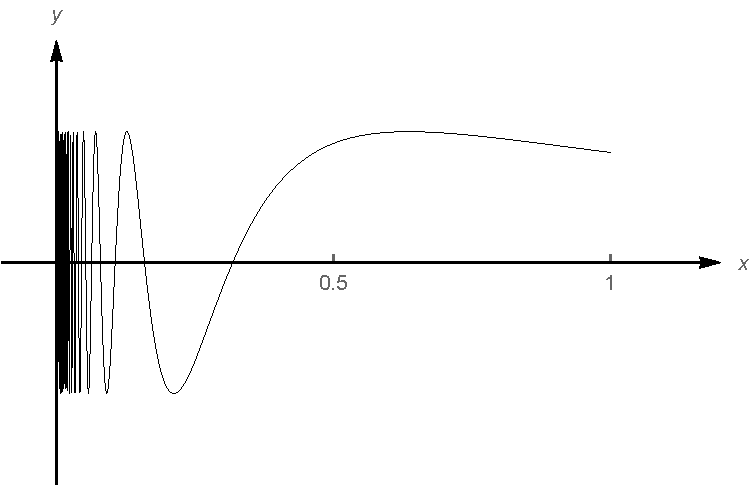
\includegraphics[scale=0.3]{Figs/sinoneoverx}
            %   \caption{Caption}
            %   \label{fig:my_label}
          \end{figure}
Let $S:=\{(x,\sin(\tfrac{1}{x}))\mid x\in (0,1]\}\cup \{(0,0)\}$ be equipped with the subset topology inherited from $\R^2$.
The space $(S,\cO_\mathrm{std}|_S)$ is connected but not path-connected.
\item \cyan{path-connected $\Rightarrow$ connected.}
      \end{itemize} 
      \item \tb{homotopic:} Two curves are homotopic if they can be continuously deformed into one another. Formally, let $(M, \mathcal{O})$ be a topological space. Two curves $\gamma, \delta:[0,1] \rightarrow M$ such that:
\begin{align*}
\gamma(0)=\delta(0) \quad \text { and } \quad \gamma(1)=\delta(1)
\end{align*}
are said to be homotopic if there exists a continuous map $h:[0,1] \times[0,1] \rightarrow M$ such that for all $\lambda \in[0,1]$ :
\begin{align*}
h(0, \lambda)=\gamma(\lambda) \quad \text { and } \quad h(1, \lambda)=\delta(\lambda) .
\end{align*}
\begin{itemize}
    \item  Let $\gamma \sim \delta: \Leftrightarrow " \gamma$ and $\delta$ are homotopic". Then, $\sim$ is an \tb{equivalence relation}.
\end{itemize}
\begin{figure}[h!]
\centering
\begin{tikzpicture}[scale=0.3]

\draw  plot[smooth, tension=.999] coordinates {(-3,-0.5) (-2,1) (-0.5,0.5) (1,0) (2.5,0.5) (3.5,1.5) (4.5,3) (6,3) (7.5,2)};

\draw  plot[smooth, tension=.999] coordinates {(-3,-0.5) (-1,-2) (1,-2.5) (3.5,-3) (5,-2.5) (6,-1.5) (7,0.5) (7.5,2)};

\draw[dashed]  plot[smooth, tension=.999] coordinates {(-3,-0.5) (-2,0.5) (-0.5,-0.5) (1,-0.5) (2.5,0) (4,1) (4.5,2) (6,2) (7.5,2)};

\draw[dashed]  plot[smooth, tension=.999] coordinates {(-3,-0.5) (-2,-0.5) (-0.5,-1) (1,-1) (2.5,-1.5) (3.5,-1) (4.5,-0.5) (5.5,0.5) (6.5,1.5) (7.5,2)};

\draw[dashed]  plot[smooth, tension=.999] coordinates {(-3,-0.5) (-1,-1.5) (1,-2) (3.5,-2.5) (4.5,-2) (6,-0.5) (6.5,1) (7.5,2)};

\draw[fill=black]  (-3,-0.5) circle (0.15);
\draw[fill=black]  (7.5,2) circle (0.15);
\node at (-3.3,-1.2) {$p$};
\node at (8,1.5) {$q$};
\node at (-1.5,1.5) {$\g$};
\node at (2,-0.9) {$h$};
\node at (2.5,-3.5) {$\delta$};
\end{tikzpicture}
\end{figure}
\item \tb{fundamental \cyan{group}\footnote{If there exists a group isomorphism between $(G, \bullet)$ and $(H, \circ)$, we write $G\cong_{\operatorname{grp}} H$.}:} It is a group with the element being the equivalent loop and ``$+$'' being the concatenation.
\begin{itemize}
\item All the previously discussed topological properties are ``boolean-valued'', i.e.\ a topological space is either connected or not connected, and so on. The fundamental group is a ``group-valued'' property.
    \item \tb{loop:}  Let $(M, \mathcal{O})$ be a topological space. Then, for every $p \in M$, we define the space of loops at $p$ by:
$\mathscr{L}_{p}:=\{\gamma:[0,1] \rightarrow M \mid \gamma$ is continuous and $\gamma(0)=\gamma(1)\}$
\item \tb{concatenation of loop:} Let $\mathscr{L}_{p}$ be the space of loops at $p \in M$. We define the concatenation operation $*: \mathscr{L}_{p} \times \mathscr{L}_{p} \rightarrow \mathscr{L}_{p}$ by:
\begin{align*}
(\gamma * \delta)(\lambda):= \begin{cases}\gamma(2 \lambda) & \text { if } 0 \leq \lambda \leq \frac{1}{2} \\ \delta(2 \lambda-1) & \text { if } \frac{1}{2} \leq \lambda \leq 1\end{cases}
\end{align*}
\item Let $(M, \mathcal{O})$ be a topological space. The \tb{fundamental group} $\pi_{1}(p)$ of $(M, \mathcal{O})$ at $p \in M$ is the set:
\begin{align*}
\pi_{1}(p):=\mathscr{L}_{p} / \sim=\left\{[\gamma] \mid \gamma \in \mathscr{L}_{p}\right\},
\end{align*}
where $\sim$ is the homotopy equivalence relation, together with the map
\begin{align*}
\begin{aligned}
\bullet: \pi_{1}(p) \times \pi_{1}(p) & \rightarrow \pi_{1}(p) \\
(\gamma, \delta) & \mapsto[\gamma] \bullet[\delta]:=[\gamma * \delta] .
\end{aligned}
\end{align*}
\begin{enumerate}%[$\dagger$]
    \item group operator is \tb{associative}, this is from ``composition of maps is associative''.
    \item group neutral element is (the equivalence class of) the constant curve $\gamma_{e}$ defined by:
\begin{align*}
\begin{aligned}
\gamma_{e}:[0,1] & \rightarrow M \\
\lambda & \mapsto \gamma_{e}(0)=p
\end{aligned}
\end{align*}
\item \tb{inverse:} for each $[\gamma] \in \pi_{1}(p)$, the inverse under $\bullet$ is the element $[-\gamma]$, where $-\gamma$ is defined by:
\begin{align*}
\begin{aligned}
-\gamma:[0,1] & \rightarrow M \\
\lambda & \mapsto \gamma(1-\lambda)
\end{aligned}
\end{align*}
\end{enumerate}
\item Examples: 
\begin{itemize}[$\dagger$]
    \item The \tb{sphere} has the property that all the loops at any point are homotopic, hence the fundamental group (at every point) of the sphere is the trivial group:
\begin{equation*}
    \forall \, p \in S^2 : \pi_1(p) = 1:=\{[\g_e]\}.
\end{equation*}
\begin{center}
\begin{tikzpicture}[scale=0.5]
  \draw[gray,dashed] (2,0) arc (0:180:2cm and 0.7cm);
  \draw[gray] (2,0) arc (0:-180:2cm and 0.7cm);
  \draw[thick] (0,0) circle[radius=2cm];
\end{tikzpicture}
\end{center}
\item The \tb{cylinder} is defined as $C:=\R\times S^1$ equipped with the product topology.

\begin{center}
\begin{tikzpicture}[scale=0.5]
  \draw[dashed] (-3.75,0) -- (-3,0);
  \draw[dashed] (3,0) -- (3.75,0);
  \draw[dashed] (-3.5,-1.5) -- (3.5,-1.5);
  \draw[dashed] (-3.75,-3) -- (-3,-3);
  \draw[dashed] (3,-3) -- (3.75,-3);
  \draw[thick] (-3,0) -- (3,0);
  \draw[thick] (-3,-3) -- (3,-3);
  \draw[dashed,gray] (0,0) arc (90:-90:0.75cm and 1.5cm);
  \draw[gray] (0,0) arc (90:270:0.75cm and 1.5cm);
\end{tikzpicture}
\end{center}

{\scriptsize A loop in $C$ can either go around the cylinder (i.e.\ around its central axis) or not. If it does not, then it can be continuously deformed to a point (the identity loop). If it does, then it cannot be deformed to the identity loop (intuitively because the cylinder is infinitely long) and hence it is a homotopically different loop. The number of times a loop winds around the cylinder is called the \tb{winding number}. Loops with different winding numbers are not homotopic. Moreover, loops with different \emph{orientations} are also not homotopic.} We have:
\begin{equation*}
\forall \, p \in C : (\pi_1(p),\bullet) \cong_\mathrm{grp}(\Z,+).
\end{equation*}

\item 
The 2-torus is defined as the set $T^2:=S^1\times S^1$ equipped with the product topology.
\begin{center}
\begin{tikzpicture}[scale=0.5]
  \draw[thick] (-1,0) to[bend left] (1,0);
  \draw[thick] (-1.2,.1) to[bend right] (1.2,.1);
  \draw[gray] (100pt,0) arc (0:-180:100pt and 30pt);
  \draw[gray,dashed] (100pt,0) arc (0:180:100pt and 30pt);
  \draw[thick] (0,0) ellipse (100pt and 50pt);
  \draw[gray,dashed]  (0,-1.75) arc (-90:90:0.3 and 0.75);
  \draw[gray] (0,-1.75) arc (-90:-270:0.3 and 0.75);
  \end{tikzpicture}
\end{center}
A loop in $T^2$ can intuitively wind around the cylinder-like part of the torus as well as around the hole of the torus. That is, there are two independent winding numbers and hence:
\begin{equation*}
\forall \, p \in T^2 : \pi_1(p) \cong_\mathrm{grp}\Z\times \Z,
\end{equation*}
where $\Z\times \Z$ is understood as a group under pairwise addition.
\end{itemize}
\end{itemize}
\end{enumerate}

\section{Topological Manifolds and Bundles}\label{sec:topmanifold}
\adjustbox{center}{
\tikzset{LA/.style = {draw=red, % just to demonstrate, where LA is used
                      line width=#1,-{Straight Barb[length=3pt]}},
         LA/.default=1pt
        }
\begin{tikzcd}[row sep=0.5cm,column sep=0.5cm, color=black]
% b  & D\arrow[d,"\text{text}"] & b \\
\text{set} \arrow[r]& \text{topological space} \arrow[r,LA] & \text{topological manifold} \arrow[r,""] & \text{differentiable manifold}\arrow[d] \arrow[r,""] & \text{principal fibre bundle} \arrow[r,""] & \text{associated fibre bundles} \\
& & &\text{Lie group}\arrow[d, xshift=0.7ex] \arrow[ru]  &\\
& & &\text{Lie algebra}\arrow[u,xshift=-0.7ex]    &\\
\end{tikzcd}
}

A summary:
\begin{itemize}[$\blacktriangleright$]
\item We give definitions for \tb{topological manifold}, \tb{submanifold} and \tb{product manifold}.
\item A \tb{bundle} consisting \tb{total manifold space},  \tb{base manifold space} and the \tb{projection operator}. 
\item The concepts like \tb{fibre}, \tb{section}, \tb{sub-bundle}, \tb{bundle morphism} and \tb{locally trivial} are then given. 
\item We then further define \tb{fibre bundle} which locally is a product bundle with a fixed fibre $F$ for all points.
\item Finally, we view manifolds from \tb{local charts} and give the definition of \tb{atlases}.
\end{itemize}

\begin{enumerate}
    \item \tb{topological manifold}: A paracompact, Hausdorff, topological space $(M, \mathcal{O})$ is called a $d$-dimensional (topological) manifold if for every point $p \in M$ there exist a neighbourhood $U(p)$ and a \tb{homeomorphism} $x: U(p) \rightarrow x(U(p)) \subseteq \mathbb{R}^{d}$. \footnote{To define complex topological manifolds, we require that the map $x$ be a homeomorphism onto an open subset of $\mathbb{C}^{d}$.} We also write $\operatorname{dim} M=d$.
\begin{itemize}
    \item  Let $M$ be a d-dimensional manifold and let $U, V \subseteq M$ be open, with $U \cap V \neq \varnothing$. If $x$ and $y$ are two homeomorphisms
\begin{align*}
x: U \rightarrow x(U) \subseteq \mathbb{R}^{d} \quad \text { and } \quad y: V \rightarrow y(V) \subseteq \mathbb{R}^{d^{\prime}}
\end{align*}
then $d=d^{\prime}$.
This ensures that the concept of \tb{dimension is indeed well-defined}, i.e. it is the same at every point, at least on \emph{each connected component} of the manifold.
\item Examples: $\mathbb{R}^{d}$ is a $d$-dimensional manifold for any $d \geq 1$. The space $S^{1}$ is a 1-dimensional manifold while the spaces $S^{2}$, cylinder $C$ and torus $T^{2}$ are 2-dimensional manifolds.
\end{itemize}
\item \tb{submanifold:} Let $(M, \mathcal{O})$ be a topological manifold and let $N \subseteq M$. Then $\left(N,\left.\mathcal{O}\right|_{N}\right)$ is called a \tb{submanifold} of $(M, \mathcal{O})$ if it is a manifold in its own right.
\begin{itemize}
    \item Examples: The space $S^{1}$ is a submanifold of $\mathbb{R}^{2}$ while the spaces $S^{2}$, $C$ and $T^{2}$ are submanifolds of $\mathbb{R}^{3}$.
\end{itemize}
\item \tb{product manifold:} Let $\left(M, \mathcal{O}_{M}\right)$ and $\left(N, \mathcal{O}_{N}\right)$ be topological manifolds of dimension $m$ and $n$, respectively. Then, $\left(M \times N, \mathcal{O}_{M \times N}\right)$ is a topological manifold of dimension $m+n$ called the \tb{product manifold}.
\begin{itemize}
    \item Examples: $T^{2}=S^{1} \times S^{1}$; or more general $n$-dimensional manifold $T^{n}:=\underbrace{S^{1} \times S^{1} \times \cdots \times S^{1}}_{n \text { times }}$. The cylinder $C=S^{1} \times \mathbb{R}$ is a 2-dimensional product manifold.
    \item \magenta{But Möbius strip is \tb{not} a product manifold.} It is only a 2-dimensional manifold. To understand it, we need the concept \cyan{\tb{fibre bundle}  that is locally a product space}.
    \begin{center}
\begin{tikzpicture}[scale=0.8]
\begin{axis}[
    hide axis,
    view={40}{45}
]
\addplot3 [
    surf, shader=faceted interp,
    point meta=x,
    colormap={slategraywhite}{rgb=(0.89,0.89,0.89) rgb=(1,1,1)},
    samples=40,
    samples y=5,
    %z buffer=sort,
    domain=0:360,
    y domain=-0.5:0.5
] (
    {(1+0.5*y*cos(x/2)))*cos(x)},
    {(1+0.5*y*cos(x/2)))*sin(x)},
    {0.5*y*sin(x/2)});

\addplot3 [
    samples=50,
    domain=-142:184.5, % The domain needs to be adjusted manually, depending on the camera angle, unfortunately
    samples y=0,
    semithick
] (
    {cos(x)},
    {sin(x)},
    {0});
\end{axis}
\end{tikzpicture}
\end{center}
\end{itemize}
\item \tb{bundle:}  A bundle (of topological manifolds) is a triple $(E, \pi, M)$ where $E$ and $M$ are topological manifolds called the \tb{total space} and the \tb{base space} respectively, and ${\pi}$ is a \cyan{\tb{continuous}, \tb{surjective}}\footnote{recall the quotient map, but here we do not use it until ``fibre bundle''} map $\pi: E \rightarrow M$ called the \tb{projection map}.
\begin{itemize}
\item Bundle can be defined for the general topological space without assuming $E$ and $M$ are manifold. But, in this course, we focus on manifold.
    \item \tb{notation:} We will often denote the bundle $(E, \pi, M)$ by $E \stackrel{\pi}{\rightarrow} M$.
    \item \tb{fibre:} Let $E \stackrel{\pi}{\rightarrow} M$ be a bundle and let $p \in M$. Then, $F_{p}:=\operatorname{preim}_{\pi}(\{p\})$ is called the fibre at the point $p$. However, $F_p$ may vary topologically from point to point.
   \item \tb{product bundle:} Let $M$ and $N$ be manifolds. Then, the triple $(M \times N, \pi, M)$, where:
\begin{align*}
\begin{aligned}
\pi: M \times N & \rightarrow M \\
(p, q) & \mapsto p
\end{aligned}
\end{align*}
is a \tb{bundle} since (one can easily check) $\pi$ is a \emph{continuous open surjective map}. Similarly, $(M \times N, \pi, N)$ with the appropriate $\pi$, is also a \tb{bundle}. Later we will see it is a \tb{fiber bundle}.
\end{itemize}
Intuitively, the fibre at the point $p \in M$ is a set of points in $E$ (represented below as a line) attached to the point $p$. The projection map sends all the points in the fibre $F_{p}$ to the point $p$.
\begin{figure}[h!]
\centering
\begin{tikzpicture}[scale=0.5]
\draw[top color=lightergray,bottom color=white,semithick]  plot[smooth cycle, tension=.9] coordinates {(-3,1.5)(-1.5,2) (1,1.5) (3.5,-0.5) (5,-2) (2,-2) (0.5,-3)};
\node (v1) at (0,0) {};
\draw[dashed] plot[smooth, tension=.7] coordinates {(1,-1.5) (0,-1) (-0.5,-0.5) (v1)};
\draw  plot[smooth, tension=.7] coordinates {(v1) (0.5,0.5) (0.5,1) (0,2.5) (0,3.5)};
\draw[fill=black]  (v1) circle (0.08);
\node at (0.5,2.5) {$F_p$};
\node at (2.75,2) {$E$};
\node at (0.5,-0.5) {$p \in M$};
\node at (-2.5,1.5) {$M$};
\end{tikzpicture}
\end{figure}


\item \tb{(cross-) section}: Let $E \stackrel{\pi}{\rightarrow} M$ be a bundle (\tb{not restrict to fibre bundle}). A (cross-) section of the bundle is a \orange{\tb{continuous}} map $\sigma: M \rightarrow E$ such that $\pi \circ \sigma=\operatorname{id}_{M}$.
\begin{itemize}
    \item Intuitively, a section is a map $\sigma$ which sends each point $p \in M$ to some point $\sigma(p)$ in its fibre $F_{p}$, so that the projection map $\pi$ takes $\sigma(p) \in F_{p} \subseteq E$ back to the point $p \in M$.
    \begin{figure}[H]
\centering
\begin{tikzpicture}[scale=0.5]
\draw[top color=lightergray,bottom color=white,semithick]  plot[smooth cycle, tension=.99] coordinates {(-2.5,0) (0.5,1.5) (3.5,-0.5) (1.5,-2)};
\draw (0,-2.5) -- (0.3224,-1.7792);
\draw[dashed]  (0.3224,-1.7792) -- (0.9501,-0.4298);
\draw (0.9501,-0.4298)-- (2.5,3);
\node at (0.5,-2.3) {$F_p$};
\node at (1.55,-0.8) {$p \in M$};
\draw[fill=black] (0.9501,-0.4298) circle (0.05);
\draw [->] plot[smooth, tension=.7] coordinates {(1.1834,-0.5006) (2.2576,0.2354) (2.5265,1.5914) (2.3316,2.0564)};
\draw [->] plot[smooth, tension=.7] coordinates {(1.8399,2.3042) (0.7458,1.7472) (0.3281,0.872) (0.7259,-0.1226)};
\node at (0.09,0.6333) {$\pi$};
\node at (1.8,0.2) {$\s$};
\node at (-1.6612,-0.3216) {$M$};
\draw [fill=black] (2.1651,2.2555) circle (0.05);
\node at (2.8,2.3) {$\s(p)$};
\node at (-1.5,2) {$E$};
\end{tikzpicture}
\end{figure}
% \item \magenta{So, locally, any section on fibre bundle can be represented as a map from base space to the fibre. Globally it is not possible unless it is a  product product.}
\item Example: Let $(M \times F, \pi, M)$ be a \tb{product bundle}. Then, a section of this bundle is a map:
\begin{align*}
\begin{aligned}
\sigma: M & \rightarrow M \times F \\
p & \mapsto(p, s(p))
\end{aligned}
\end{align*}
where $s: M \rightarrow F$ is continuous map.
\item Note, sections may \tb{not} exist due the requirement of \orange{continuous}. See below fibre bundles. 
% }
\end{itemize}
\item \tb{sub-bundle:} A \tb{sub-bundle} of a bundle $(E,\pi,M)$ is a triple $(E',\pi',M')$ where $E'\se E$ and $M'\se M$ are submanifolds and $\pi':=\pi|_{E'}$.

\item \tb{restricted bundle:} Let $(E,\pi,M)$ be a bundle and let $N\se M$ be a submanifold. The \emph{restricted bundle} (to $N$) is the triple $(E,\pi',N)$ where:
\begin{equation*}
    \pi':=\pi|_{\mathrm{preim}_\pi(N)}
\end{equation*}
\item \cyan{\tb{bundle morphism:}}
Let $E\xrightarrow{\,\pi\,}M$ and $E'\xrightarrow{\,\pi'\,}M'$ be bundles and let $u: E\to E'$ and $v: M\to M'$ be maps. Then $(u,v)$ is called a \tb{bundle morphism} if the following diagram commutes:
\begin{equation*}
    \begin{tikzcd}
E \ar[r,"u"] \ar[d,"\pi"]& E' \ar[d,"\pi'"]\\
M \ar[r,"v"]& M'
\end{tikzcd}
\end{equation*}
\begin{itemize}
    \item \tb{uniquness:} If $(u,v)$ and $(u,v')$ are both bundle morphisms, then $v=v'$. That is, given $u$, if there exists $v$ such that $(u,v)$ is a bundle morphism, then $v$ is \tb{unique}.
    \item Later we will see for principal  fiber bundles with structure group $G$ and whose total spaces are (right) $G$-spaces, bundle morphisms are also required to be $G$-equivariant on the fibers.
\end{itemize}

\item \cyan{\tb{bundle isomorphic: }} Two bundles $E\xrightarrow{\,\pi\,}M$ and $E'\xrightarrow{\,\pi'\,}M'$ are said to be \tb{isomorphic (as bundles)}  if there exist bundle morphisms $(u,v)$ and $(u^{-1},v^{-1})$ satisfying:
\begin{equation*}
\begin{tikzcd}
E \ar[rr,shift left,"u"] \ar[dd,"\pi"']&& E' \ar[ll,shift left,"u^{-1}"]\ar[dd,"\pi'"]\\
&&\\
M \ar[rr,shift left,"v"]&& M' \ar[ll,shift left,"v^{-1}"]
\end{tikzcd}
\end{equation*}
Such a $(u,v)$ is called a \emph{bundle isomorphism}
\begin{itemize}
    \item \cyan{Bundle isomorphisms are the structure-preserving maps for bundles.}
    \item \tb{notation:}  We write $E\xrightarrow{\,\pi\,}M  \cong_{\mathrm{bdl}} E'\xrightarrow{\,\pi'\,}M'$.
\end{itemize}

\item \tb{locally isomorphic:} 
A bundle $E\xrightarrow{\,\pi\,}M$ is said to be {locally isomorphic (as a bundle)} to a bundle $E'\xrightarrow{\,\pi'\,}M'$ if for all $p\in M$ there exists a neighbourhood $U(p)$ such that the restricted bundle:
\begin{equation*}
\mathrm{preim}_\pi(U(p))\xrightarrow{\,\pi|_{\mathrm{preim}_\pi(U(p))}\,}U(p)
\end{equation*}
is isomorphic to the bundle $E'\xrightarrow{\,\pi'\,}M'$.
\item \tb{trivial; locally trivial:} A bundle $E\xrightarrow{\,\pi\,}M$ is said to be:
\begin{itemize}
    \item \emph{trivial} if it is isomorphic to a product bundle;
    \item \emph{locally trivial} if it is locally isomorphic to a product bundle (It is a fibre bundle. See below for more details).
    \item Examples: 
    \begin{itemize}[$\dagger$]
        \item The cylinder $C$ is trivial as a bundle, and hence also locally trivial. 
        \item The M\"obious strip is not trivial but it is locally trivial.
    \end{itemize}
\end{itemize}

\item \tb{pull-back bundle:} 
Let $E\xrightarrow{\,\pi\, }M$ be a bundle and let $f: M'\to M$ be a map from some manifold $M'$. The \tb{pull-back bundle} of $E\xrightarrow{\,\pi\, }M$ \emph{induced by} $f$ is defined as $E'\xrightarrow{\,\pi'\,}M'$, where:
\begin{equation*}
E':=\{(m',e)\in M'\times E \mid f(m')=\pi(e)\}
\end{equation*}
and $\pi' (m',e) := m'$.
\begin{itemize}
    \item If $E'\xrightarrow{\,\pi'\,}M'$ is the pull-back bundle of $E\xrightarrow{\,\pi\, }M$ induced by $f$, then one can easily construct a \tb{bundle morphism} by defining:
    \begin{align*}
        u : & E'  \to  E\\
& (m',e)  \mapsto  e
    \end{align*}
    This corresponds to the diagram:
    \begin{equation*}
\begin{tikzcd}
E' \ar[d,"\pi'"] \ar[r,"u"] & E\ar[d,"\pi"]\\
M' \ar[r,"f"]& M
\end{tikzcd}
    \end{equation*}
    \item \tb{pull back of section:}  Let $E'\xrightarrow{\,\pi'\,}M'$ be the pull-back bundle of $E\xrightarrow{\,\pi\, }M$ induced by $f$.
\begin{equation*}
\begin{tikzcd}
E' \ar[dd,shift left,"\pi'"] && E\ar[dd,shift left,"\pi"]\\
&&\\
M' \ar[uurr,"\s\circ f"]\ar[uu,shift left,"\s'"]\ar[rr,"f"]&& M\ar[uu,shift left,"\s"]
\end{tikzcd}
 \end{equation*}
If $\s$ is a section of $E\xrightarrow{\,\pi\, }M$, then $\s \circ f$ determines a map from $M'$ to $E$ which sends each $m'\in M'$ to $\s(f(m')) \in E$. However, since $\s$ is a section, we have:
\begin{equation*}
\pi(\s(f(m'))= (\pi \circ \s \circ f)(m') = (\id_M\circ f)(m') = f(m')
   \end{equation*}
and hence $(m',(\s \circ f)(m'))\in E'$ by definition of $E'$. Moreover:
\begin{equation*}
\pi' (m',(\s \circ f)(m')) = m'
 \end{equation*}
and hence the map:
    \begin{align*}
\s' : & M'  \to  E'\\
& m' \mapsto  (m',(\s \circ f)(m'))
    \end{align*}
satisfies $\pi'\circ\s'=\id_{M'}$ and it is thus \tb{a section on the pull-back bundle} $E'\xrightarrow{\,\pi'\,}M'$.
\end{itemize}


\item \tb{fibre bundle:} Let $E \stackrel{\pi}{\rightarrow} M$ be a bundle and let $F$ be a manifold. Then, $E \stackrel{\pi}{\rightarrow} M$ is called a fibre bundle, with (typical) \tb{fibre $F$}, if we have, roughly speaking,
\begin{align*}
\forall p \in M: F_p\coloneqq \operatorname{preim}_{\pi}(\{p\}) \cong_{\text {top }} F .
\end{align*}
More strictly speaking, if it  satisfies the local triviality condition:
\begin{itemize}
    \item We require that for every $p \in M$, there is an open neighborhood $U \subseteq M$ of $p$ (which will be called a \tb{trivializing neighborhood}) such that there is a \tb{homeomorphism} $\varphi: \pi^{-1}(U) \rightarrow U \times F$ (where $\pi^{-1}(U)$ is given the subspace topology, and $U \times F$ is the product space) in such a way that $\pi$ agrees with the projection onto the first factor. That is, the following diagram should \tb{commute} (i.e. it is a \cyan{\tb{local isomorphism}}):
    \begin{figure}[H]
              \centering
              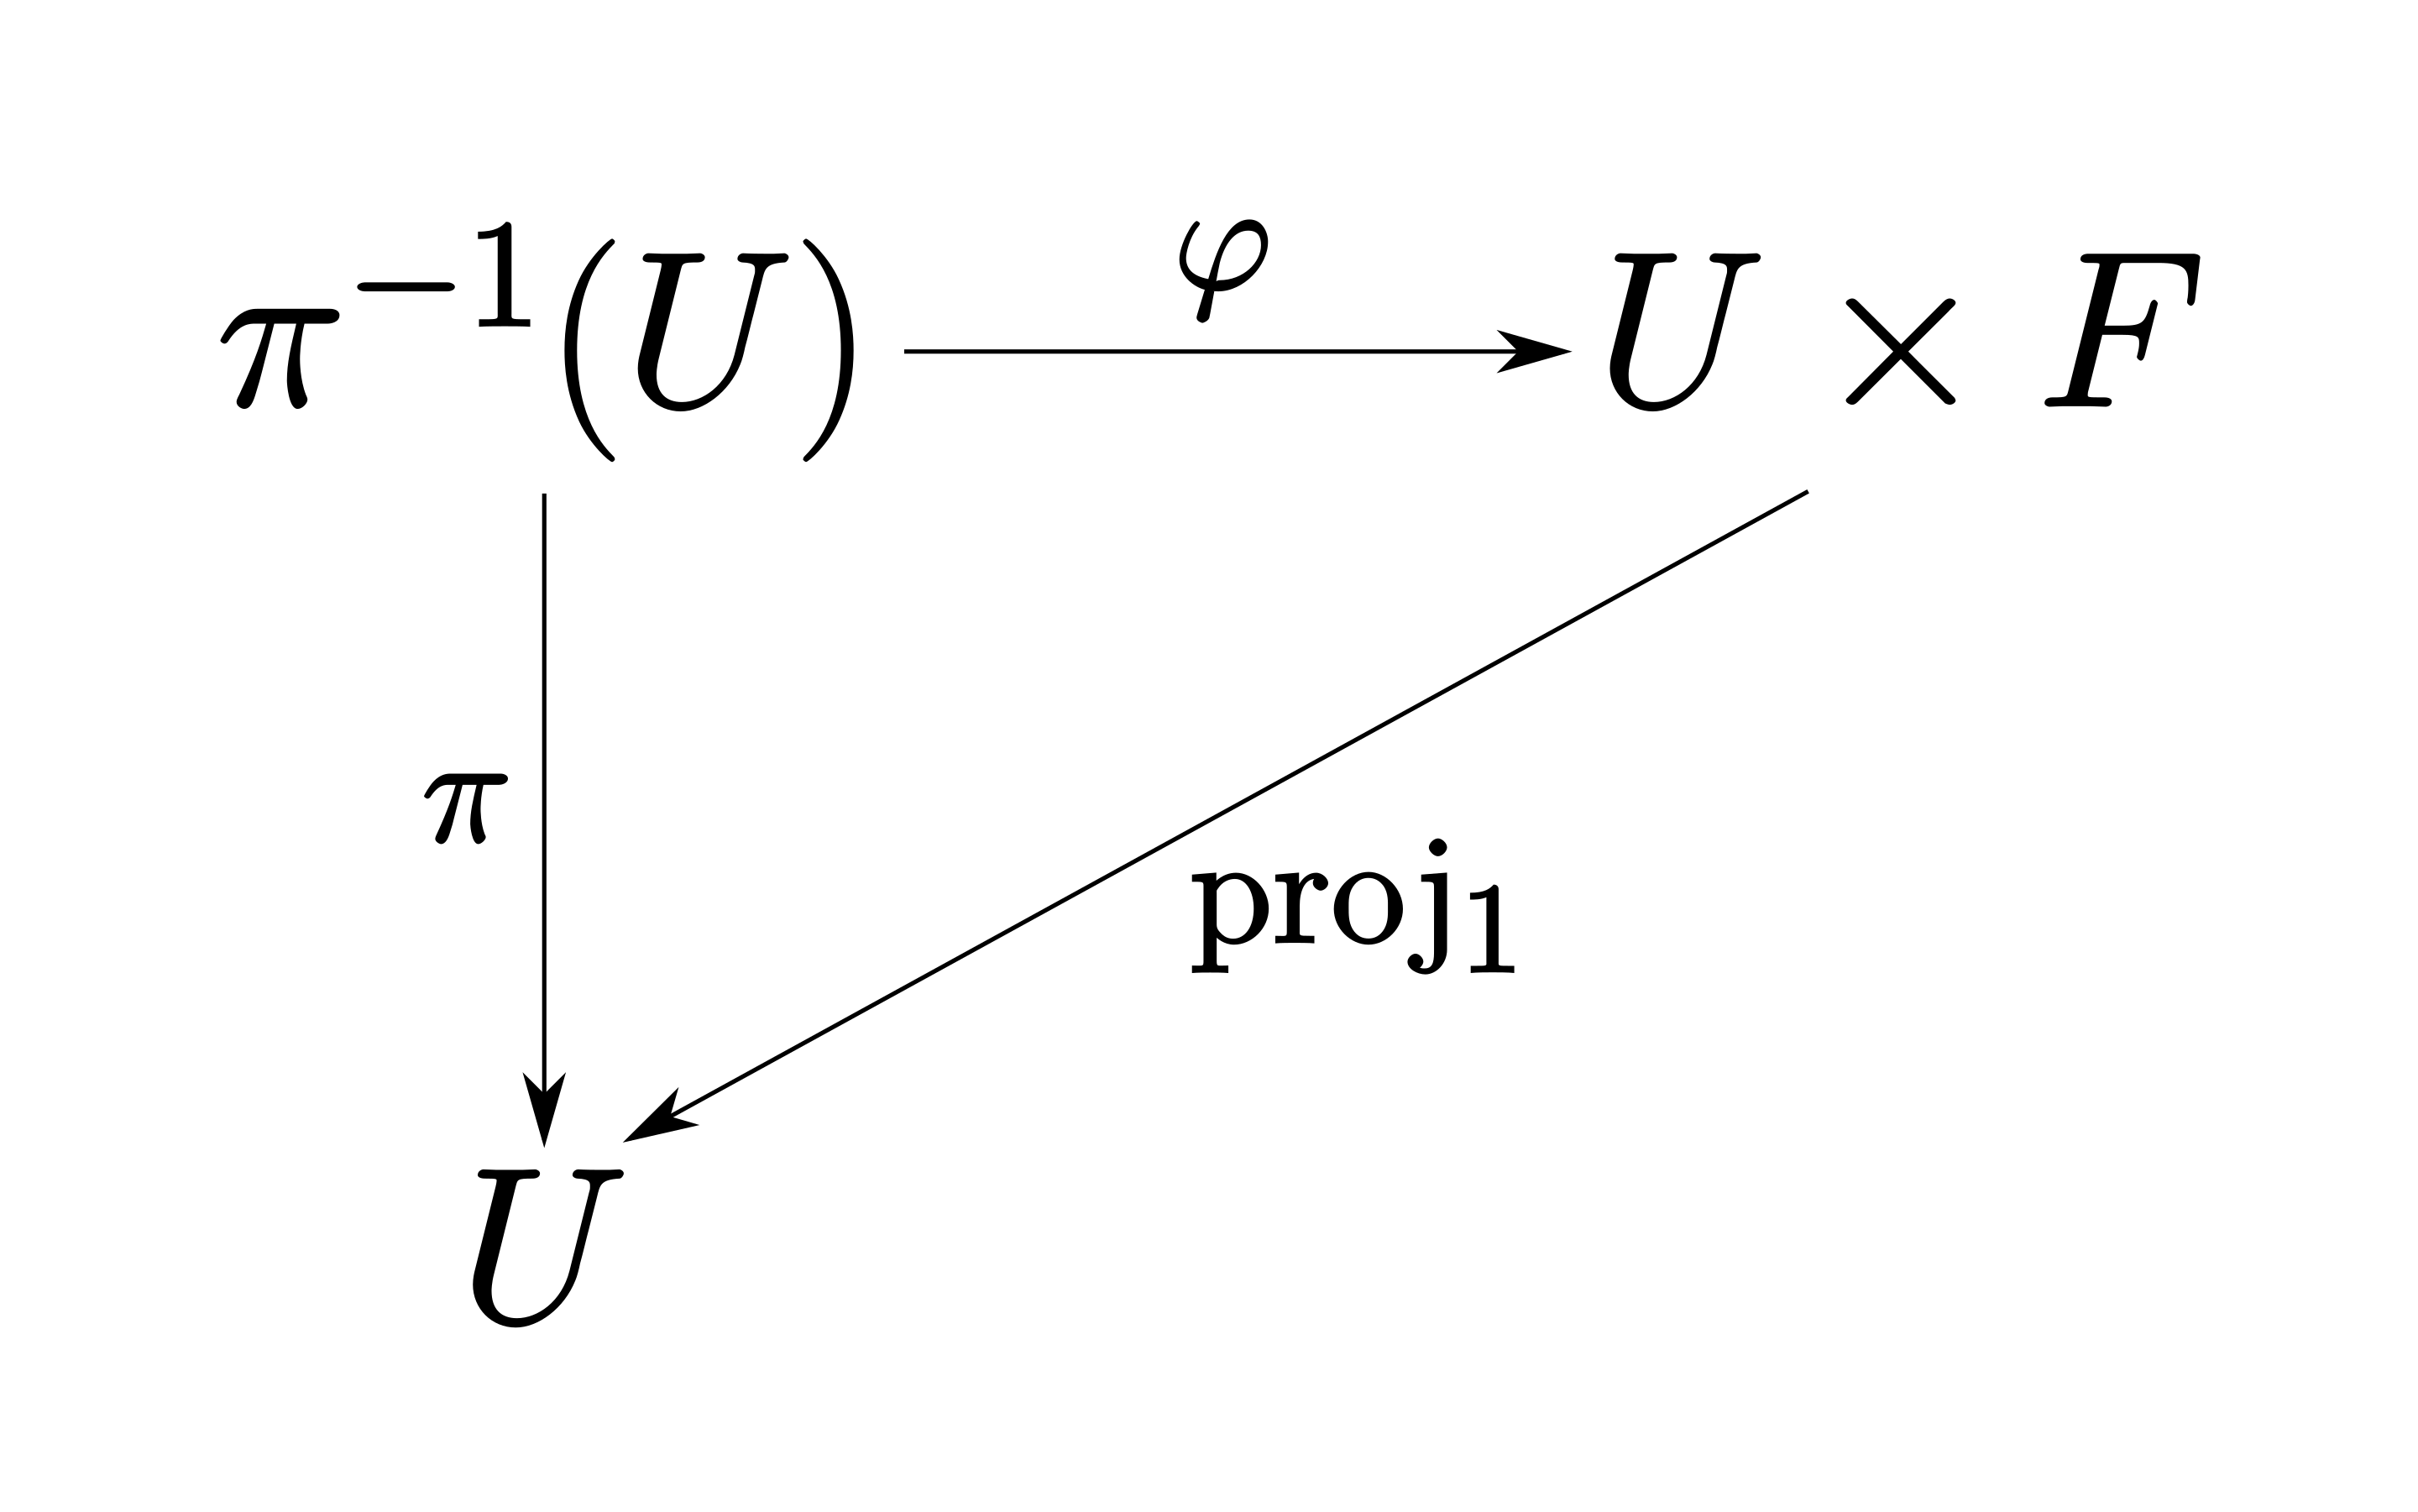
\includegraphics[scale=0.04]{Figs/5.png}
          \end{figure}
      where $\operatorname{proj}_{1}: U \times F \rightarrow U$ is the \tb{natural projection} and $\varphi: \pi^{-1}(U) \rightarrow U \times F$ is a \tb{homeomorphism}. The set of all $\left\{\left(U_{i}, \varphi_{i}\right)\right\}$ is called a \tb{local trivialization} of the bundle.    
      
     \item Thus, for any $p \in B$, the preimage $\pi^{-1}(\{p\})$ is \tb{homeomorphic} to $F$ (since this is true of $\operatorname{proj}_{1}^{-1}(\{p\})$). Every fiber bundle $\pi: E \rightarrow M$ is an \tb{continuous open map}, since projections of products are open maps and $\varphi$ is a homeomorphism. Therefore $M$ carries the \cyan{\tb{quotient topology}} determined by the map $\pi$.
     \item \tb{notation:}
A fiber bundle  is often denoted
\begin{align*}
F \longrightarrow E \stackrel{\pi}{\longrightarrow} M
\end{align*}
\item A \tb{smooth fiber bundle} is a fiber bundle in the category of smooth\footnote{Definition of smooth is listed in \cref{sec:diff}} manifolds. That is, $E, M$, and $F$ are required to be smooth manifolds and all the functions above are required to be smooth maps. 

\item \tb{product bundle is a \tb{fiber bundle}} since (one can easily check) $\pi$ is a \emph{continuous open surjective map}. Similarly, $(M \times N, \pi, N)$ with the appropriate $\pi$, is also a \tb{fiber bundle}.

\centerline{\magenta{``product bundle (i.e. manifold)'' $\subseteq$ fibre bundle $\subseteq$ bundle}}

\item Example I: The Möbius strip is a fibre bundle $F \longrightarrow E \stackrel{\pi}{\rightarrow} S^{1}$, with fibre $F:=[0,1]$, where $E \neq S^{1} \times[0,1]$, i.e. the Möbius strip is not a product bundle.
\item Example II: This hairbrush is like a fiber bundle in which the base space is a cylinder and the fibers (bristles) are line segments. The mapping $\pi\cl E\to B$ would take a point on any bristle and map it to its root on the cylinder.
\begin{figure}[H]
    \centering
    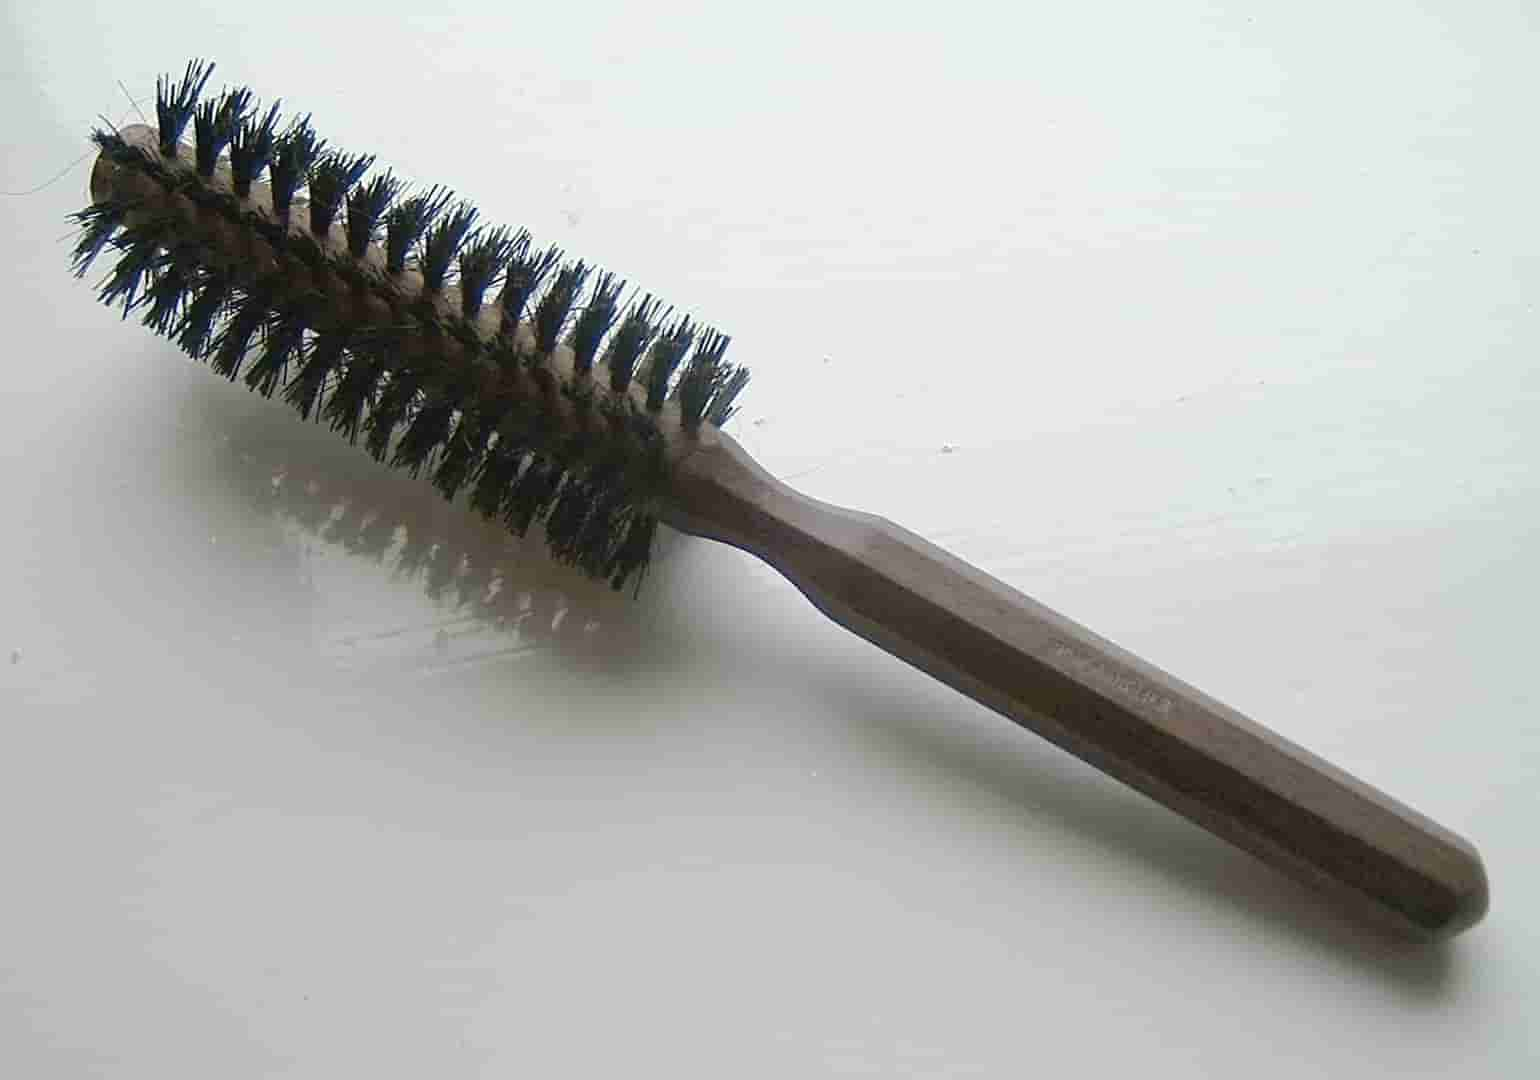
\includegraphics[scale=0.08]{Figs/Roundhairbrush.jpg}
    % \caption{Caption}
    % \label{fig:my_label}
\end{figure}
\item \magenta{\tb{important clarification:} Fiber bundles do \tb{not} in general have such \tb{global sections}. But locally, since we have the locally trivial, we can always define a  \tb{local section} of a fiber bundle. Locally it is a continuous map $s: U \rightarrow E$ where $U$ is an open set in $B$ and $\pi(s(x))=x$ for all $x$ in $U$. If $(U, \varphi)$ is a local trivialization of $E$, where $\varphi$ is a homeomorphism from $\pi^{-1}(U)$ to $U \times F$ (where $F$ is the fiber), then local sections always exist over $U$ in bijective correspondence with continuous maps from $U$ to $F$.
\begin{itemize}[$\ast$]
    \item What is hidden behind is that there is \green{\tb{no canonical way to identify the fibers.}}  We only have each $F_p$ \tb{topologically equals} $F$, i.e.,
$\forall p \in M: \operatorname{preim}_{\pi}(\{p\}) \cong_{\text {top }} F.$
    In the very definition of fiber bundle, close fibers are identified to each other thanks to \tb{local trivializations.} But there is \tb{no global identification.}
    \item To define a continuous function, we only need to prescribe its behavior on an open covering, if we make sure that the definitions coincide with each other on the intersections(that is the glueing). Now, if we have a fiber bundle, we are given an open cover of $B$, say $B=\cup_i U_i$, and isomorphisms $\phi_i: \pi^{-1}\left(U_i\right) \rightarrow U_i \times F$. So when you are checking the compatibility condition on $U_i \cap U_j$, you have to remember that you used the $\phi_i$ to define your section. That means you have used \tb{different trivial neighbouhoods} covering $B$.
    \item  Example: the fiber bundle over $S^1$ with fiber $F=\mathbb{R} \backslash\{0\}$ obtained by taking the Möbius bundle and removing the zero section do not in general have global sections.
    \item So, locally, any section on fibre bundle can be represented as a map from base space to the fibre $F$. Globally it may not be always possible unless, for example, it is a  \tb{product product.}
    \item A principal bundle has a global section if and only if it is trivial (See \cref{sec:principal}). On the other hand, a vector bundle (i.e., an associated bundle with each fibre carrying a vector space structure, e.g. the tensor bundle, see \cref{sec:parall}) always has a global section, namely the \tb{zero section}. However, it only admits a nowhere vanishing section if its Euler class is zero. See also \tb{hairy ball theorem} in \cref{sec:tensorII}.  
\end{itemize}}

% (consider, for example, the fiber bundle over $S^1$ with fiber $F=\mathbb{R} \backslash\{0\}$ obtained by taking the Möbius bundle and removing the zero section), so it is also useful to define sections only locally. 

% The (local) sections form a sheaf over $B$ called the sheaf of sections of $E$.




\end{itemize}



\item \tb{viewing manifolds from atlases:}
\begin{enumerate}
    \item \tb{chart:}
Let $(M,\cO)$ be a $d$-dimensional manifold. Then, a pair $(U,x)$ where $U\in \cO$ and $x: U \to x(U) \se \R^d$ is a homeomorphism, is said to be a \emph{chart} of the manifold.
\item \tb{component functions:}

The \tb{component functions (or maps)} of $x: U\to x(U) \se \R^d$ are the maps:
    \begin{align*}
x^i : & U   \to  \Real \\
& p  \mapsto  \proj_i(x(p))
    \end{align*}
for $1\leq i\leq d$, where $\mathrm{proj}_i(x(p))$ is the $i$-th component of $x(p)\in \R^d$. The $x^i(p)$ are called the \emph{coordinates} of the point $p\in U$ \gls{wrt} the chart $(U,x)$.
\item \tb{atlas}
An \emph{atlas} of a manifold $M$ is a collection $\mathscr{A}:=\{(U_\a,x_\a)\mid \a \in \mathcal{A}\}$ of charts such that:
\begin{equation*}
\bigcup_{\a \in \mathcal{A}}U_\a = M. 
\end{equation*}

\item \tb{chart transition map:}
For two charts $(U,x)$ and $(V,y)$ are said to be \emph{$\mathcal{C}^0$-compatible} if  $U \cap V = \vn$
\begin{equation*}
y\circ x^{-1}: x(U\cap V) \to y(U\cap V)
\end{equation*}
is continuous.

Note that $y\circ x^{-1}$ is a map from a subset of $\R^d$ to a subset of $\R^d$.
\begin{equation*}
\begin{tikzcd}
& U\cap V \se M \ar[ldd,"x"'] \ar[rdd,"y"]&\\
&&&\\
x(U\cap V) \se \R^d \ar[rr,"y\circ x^{-1}"']& & y(U\cap V)\se \R^d
\end{tikzcd}
\end{equation*}
\item 
The map $y\circ x^{-1}$ (and its inverse $x\circ y^{-1}$) is called the \emph{coordinate change map} or \emph{chart transition map}.
\item \tb{various compatible:} See my riemannian manifold notes and next \cref{sec:diff}. In this section we only consider $\mathcal{C}^0$-compatibility.
\item \tb{maximal $\mathcal{C}^0$ atlas:}
A $\mathcal{C}^0$-atlas $\mathscr{A}$ is said to be a \tb{maximal atlas} if for every $(U,x)\in\mathscr{A}$, we have $(V,y)$  must be in $\mathscr{A}$ for all $(V,y)$ charts that are $\mathcal{C}^0$-compatible with $(U,x)$.
\item \cyan{\tb{two point of view:}}
We can now look at ``objects on'' topological manifolds from two points of view. For instance, consider a curve on a $d$-dimensional manifold $M$, i.e.\ a map $\g: \R\to M$. We now ask whether this curve is continuous, as it should be if models the trajectory of a particle on the ``physical space'' $M$.
\begin{enumerate}[i).]
    \item \tb{from topology:} A first answer is that $\g: \R \to M$ is continuous if it is continuous as a map between the \tb{topological spaces} $\R$ and $M$.
    \item  \tb{from local representation:} Secondly, we consider only a portion (open subset $U$) of the physical space $M$ and, instead of studying the map $\g:\mathrm{preim}_\g(U)\to U$ directly, we study the map:
\begin{equation*}
x\circ \g: \mathrm{preim}_\g(U) \to x(U) \se \R^d,
\end{equation*}
where $(U,x)$ is a chart of $M$. More likely, you would be checking the continuity of the coordinate maps $x^i\circ \g$, which would then imply the continuity of the ``real'' curve $\g:\mathrm{preim}_\g(U)\to U$ (real, as opposed to its coordinate representation).
\end{enumerate}
\begin{itemize}
    \item You may chose a different chart $(U,y)$ and then study the coordinate map $y\circ \g$. Notice that some results (e.g.\ the continuity of $\g$) obtained in the previous chart $(U,x)$ can be immediately ``transported'' to the new chart $(U,y)$ via the chart transition map $y\circ x^{-1}$. Intuitively speaking, the map $y\circ x^{-1}$ allows us to just use representation to study the real world without worries.
\begin{equation*}
\begin{tikzcd}
&& y(U)\se\R^d\\
&&\\
\mathrm{preim}_\g(U)\se\R \ar[rr,"\g"] \ar[ddrr,"x\circ \g"] \ar[uurr,"y\circ \g"]&& U\se M \ar[dd,"x"] \ar[uu,"y"'] \\
&&\\
&& x(U)\se\R^d \ar[uuuu,bend right=65,"y\circ x^{-1}"']
\end{tikzcd}
\end{equation*}
\end{itemize}

\end{enumerate}
\end{enumerate}




\section{Differentiable Structures: Definition and Classification}\label{sec:diff}

\adjustbox{center}{
\tikzset{LA/.style = {draw=red, % just to demonstrate, where LA is used
                      line width=#1,-{Straight Barb[length=3pt]}},
         LA/.default=1pt
        }
\begin{tikzcd}[row sep=0.5cm,column sep=0.5cm, color=black]
% b  & D\arrow[d,"\text{text}"] & b \\
\text{set} \arrow[r]& \text{topological space} \arrow[r] & \text{topological manifold} \arrow[r,LA] & \text{differentiable manifold}\arrow[d] \arrow[r,""] & \text{principal fibre bundle} \arrow[r,""] & \text{associated fibre bundles} \\
& & &\text{Lie group}\arrow[d, xshift=0.7ex] \arrow[ru]  &\\
& & &\text{Lie algebra}\arrow[u,xshift=-0.7ex]    &\\
\end{tikzcd}
}

We now add more structures to vanilla topological manifold and define the \tb{differentiable manifold}.
\begin{enumerate}
    \item \tb{adding ${\scalebox{0.75}\FiveFlowerOpen}$-compatibility  by refining the (maximal) $\calC^0$ atlas:}  
An atlas $\mathscr{A}$ for a topological manifold is called a {\scalebox{0.75}\FiveFlowerOpen}-\tb{atlas} if any two charts $(U,x), (V,y) \in \mathscr{A}$ are {\scalebox{0.75}\FiveFlowerOpen}-compatible. In other words, either $U\cap V = \vn$ or if $U\cap V \neq \vn$, then the transition map $y\circ x^{-1}$ from $x(U\cap V)$ to $y(U\cap V)$ must be {\scalebox{0.75}\FiveFlowerOpen}.
\begin{equation*}
    \begin{tikzcd}
& U\cap V \se M \ar[ldd,"x"'] \ar[rdd,"y"]&\\
&&&\\
x(U\cap V) \se \R^{\dim M} \ar[rr,"y\circ x^{-1}"']& & y(U\cap V)\se \R^{\dim M}
\end{tikzcd}
\end{equation*}
The symbol {\scalebox{0.75}\FiveFlowerOpen} is being used as a placeholder for any of the following:
\begin{itemize}
\item ${\scalebox{0.75}\FiveFlowerOpen} = \mathcal{C}^0$: this just reduces to the previous definition;
\item ${\scalebox{0.75}\FiveFlowerOpen} = \mathcal{C}^k$: the transition maps are $k$-times continuously differentiable as maps between open subsets of $\R^{\dim M}$;
\item ${\scalebox{0.75}\FiveFlowerOpen} = \mathcal{C}^\infty$: the transition maps are \tb{smooth}; equivalently, the atlas is $\mathcal{C}^k$ for all $k\geq 0$;
\item ${\scalebox{0.75}\FiveFlowerOpen} = \mathcal{C}^\omega$: the transition maps are \tb{(real) analytic}, which is stronger than being smooth;
\item ${\scalebox{0.75}\FiveFlowerOpen} =$ complex: if $\dim M$ is even, $M$ is a \tb{complex manifold} if the transition maps are continuous and satisfy the Cauchy-Riemann equations.
\end{itemize}
\item \tb{differentiable manifold:} When we say differentiable manifold, we mean a $d$-dimensional (topological) manifold together with a \tb{maximal differentiable atlas}\footnote{``maximal'' is defined similar to  \cref{sec:topmanifold} with ${\scalebox{0.75}\FiveFlowerOpen}$-compatibility requirement between any two charts.} on it.
\begin{itemize}
\item Note differentiable manifolds are equipped \tb{maximal} differentiable atlas.
    \item \tb{$\mathcal{C}^k$-manifold:} A $\mathcal{C}^k$\emph{-manifold}\index{manifold} is a triple $(M,\cO,\mathscr{A})$, where $(M,\cO)$ is a topological manifold and $\mathscr{A}$ is a \tb{maximal} $\mathcal{C}^k$-atlas. 
\item \tb{smooth manifold:}  it has a \tb{maximal} $\mathcal{C}^\infty$-atlas.
\end{itemize}


\item \tb{Whitney theorem:} Any maximal $\mathcal{C}^k$-atlas, with $k\geq 1$, contains a $\mathcal{C}^\infty$-atlas. Moreover, any two maximal $\mathcal{C}^k$-atlases that contain the same $\mathcal{C}^\infty$-atlas are identical.
\begin{itemize}
    \item An immediate implication is that if we can find a $\mathcal{C}^1$-atlas for a manifold, then we can also assume the existence of a $\mathcal{C}^\infty$-atlas for that manifold simply by removing charts, keeping only the ones which are $\mathcal{C}^\infty$-compatible.. 
    \item This is not the case for topological manifolds in general: a space with a $\mathcal{C}^0$-atlas may not admit any $\mathcal{C}^1$-atlas.
   \item  For the purposes of this, in this course we will not distinguish between $\mathcal{C}^k$ ($k\ge 1$) and $\mathcal{C}^\infty$-manifolds in the above sense.
    \item But \cyan{two different $\mathcal{C}^k$ maximal atlas must carry  different $\mathcal{C}^\infty$-atlas.} See below for the existence of two different (i.e. incompatible) $\mathcal{C}^k$ maximal atlas.
\end{itemize}
 \item \tb{compatible atlases:} Two {\scalebox{0.75}\FiveFlowerOpen}-atlases $\mathscr{A}$, $\mathscr{B}$ are \tb{compatible} if their union $\mathscr{A}\cup\mathscr{B}$ is again a {\scalebox{0.75}\FiveFlowerOpen}-atlas, and are incompatible otherwise.
{\tiny Alternatively, we can define the compatibility of two atlases in terms of the compatibility of any pair of charts, one from each atlas.}
\begin{itemize}
    \item A given topological manifold can \cyan{\tb{carry different incompatible atlases.}}
    \item Example: Let $(M,\cO)=(\R,\cO_\mathrm{std})$. Consider the two atlases $\mathscr{A}=\{(\R,\id_\R)\}$ and $\mathscr{B}=\{(\R,x)\}$, where $x: a \mapsto \sqrt[3]{a}$. Since they both contain a single chart, the compatibility condition on the transition maps is easily seen to hold (in both cases, the only transition map is $\id_\R$). Hence they are both $\mathcal{C}^\infty$-atlases.

Consider now $\mathscr{A}\cup\mathscr{B}$. The transition map $\id_\R\circ x^{-1}$ is the map $a\mapsto a^3$, which is smooth. However, the other transition map, $x\circ\id_\R^{-1}$, is the map $x$, which is not even differentiable once (the first derivative at $0$ does not exist). Consequently, $\mathscr{A}$ and $\mathscr{B}$ are not even $\mathcal{C}^1$-compatible. But later we will see they are the same \tb{up to diffeomorphism}
\end{itemize} 
    
    \item \tb{differentiable (or even smooth) map between manifolds:} Let $\phi: M\to N$ be a map, where $(M,\cO_M,\mathscr{A}_M)$ and $(N,\cO_N,\mathscr{A}_N)$ are $\mathcal{C}^k$ (or even $\mathcal{C}^\infty$)-manifolds. Then $\phi$ is said to be ($\mathcal{C}^k$-)\emph{differentiable at} $p\in M$ if for some charts $(U,x)\in\mathscr{A}_M$ with $p\in U$ and $(V,y)\in\mathscr{A}_N$ with $\phi(p)\in V$, the map $y\circ\phi\circ x^{-1}$ is $k$-times continuously differentiable at $x(p)\in x(U)\se\R^{\dim M}$ in the usual sense.
\begin{equation*}
\begin{tikzcd}
U\se M \ar[rr,"\phi"] \ar[dd,"x"] && V\se N \ar[dd,"y"]\\
&&\\
x(U)\se\R^{\dim M}\ar[rr,"y\circ\phi\circ x^{-1}"] && y(V)\se\R^{\dim N}
\end{tikzcd}
\end{equation*}

\begin{itemize}
    \item The definition of differentiability is well-defined by using the following diagram:

\begin{equation*}
\begin{tikzcd}
\widetilde x(U\cap\widetilde U)\se\R^{\dim M}\ar[rr,"\widetilde y\circ\phi\circ \widetilde x^{-1}"] && \widetilde y(V\cap\widetilde V)\se\R^{\dim N}\\
&&\\
U\cap\widetilde U\se M \ar[rr,"\phi"] \ar[dd,"x"] \ar[uu,"\widetilde x"'] && V\cap\widetilde V\se N \ar[dd,"y"] \ar[uu,"\widetilde y"']\\
&&\\
x(U\cap\widetilde U)\se\R^{\dim M}\ar[rr,"y\circ\phi\circ x^{-1}"] \ar[uuuu,bend left=70,"\widetilde x\circ x^{-1}"]&& y(V\cap\widetilde V)\se\R^{\dim N} \ar[uuuu,bend right=70,"\widetilde y\circ y^{-1}"']
\end{tikzcd}
\end{equation*}
\item \tb{Special examples:} Let $(M,\cO,\mathscr{A})$ be a $d$-dimensional smooth manifold and let $(U,x)\in\mathscr{A}$. Then $x: U \to x(U)\se \R^d$ is smooth map (between manifolds):
\begin{equation*}
\begin{tikzcd}
U \ar[rrr,"x"] \ar[dd,"y"] &&& x(U) \ar[dd,"\id_{x(U)}"]\\
&&\\
x(U)\se\R^{d} \ar[rrr,"\id_{x(U)}\circ x\circ y^{-1}"]&&& x(U)\se\R^{d} 
\end{tikzcd}
\end{equation*}
Note, here we view both $U$ and $x(U)$ as the submanifold of $M$ and $\Real^d$ respectively. $x: U \to x(U)$ is smooth since the map $\id_{x(U)}\circ x\circ y^{-1}$ is smooth. Note here $y$ is a chart that overlaps with $x$. Similarly, the coordinate maps $x^i:={\proj_i}\circ x: U \to \R$ are also smooth from $U$ to $\Real$. 
\end{itemize}
\item \tb{diffeomorphism:} 
Let $\phi: M \to N$ be a \tb{bijective} map between \tb{smooth} manifolds. If both $\phi$ and $\phi^{-1}$ are smooth, then $\phi$ is said to be a \tb{diffeomorphism}.
\begin{itemize}
    \item \cyan{Diffeomorphisms are the structure preserving maps between smooth manifolds.} 
    \item \tb{notation:} Two manifolds $(M,\cO_M,\mathscr{A}_M)$, $(N,\cO_N,\mathscr{A}_N)$ are said to be \emph{diffeomorphic} if there exists a diffeomorphism $\phi: M\to N$ between them. We write $M \cong_\text{diff}N$.
    \item  It is customary to consider diffeomorphic manifolds to be \tb{the same} from the point of view of differential geometry. {\tiny Being diffeomorphic is an equivalence relation. This is similar to the situation with topological spaces, where we consider homeomorphic spaces to be the same from the point of view of topology. This is typical of all structure preserving maps.}
\end{itemize}

\item \tb{classification of differentiable structures}: How many smooth structures on a given topological space are there, \tb{up to diffeomorphism}? It depends on the \magenta{dimension} of the manifold!

\begin{itemize}
    \item Let $M$ be a manifold with $\dim M = 1, 2$, or $3$. Then there is a unique smooth structure on $M$ up to diffeomorphism. 
    \begin{itemize}[$\ast$]
        \item Recall we showed that we can equip $(\R,\cO_\mathrm{std})$ with two incompatible atlases $\mathscr{A}$ and $\mathscr{B}$. Let $\mathscr{A}_\mathrm{max}$ and $\mathscr{B}_\mathrm{max}$ be their extensions to maximal atlases. Clearly, these are different manifolds, because the atlases are different, but since $\dim \R=1$, they must be diffeomorphic.
    \end{itemize}
    \item \tb{surgery theory:} {\tiny This is a collection of tools and techniques in topology with which one obtains a new manifold from given ones by performing surgery on them, i.e.\ by cutting, replacing and gluing parts in such a way as to control topological invariants like the fundamental group.} There are only \tb{finitely many} smooth manifolds (up to diffeomorphism) one can make from a topological manifold if $\dim M > 4$.
    \begin{itemize}[$\ast$]
        \item For $\dim M = 4$ there are infinitely many:  If $M$ is a non-compact topological manifold, then there are uncountably many non-diffeomorphic smooth structures; In the compact case there are partial results to give infinitely many.
    \end{itemize}
\end{itemize}
\end{enumerate}


\section{Tensor Space Theory I: Over A Field}\label{sec:tensorI}
A summary:
\begin{itemize}[$\blacktriangleright$]
\item We give the definition of \tb{vector space} and \tb{linear (isomorphism) map}.
\item We definite special nonlinear maps called \tb{bilinear map} and more general \tb{multilinear map} over Cartesian product of vector spaces.
\item \tb{Tensor} and \tb{tensor space} (a vector space) is then defined.
\item We give the definition of \tb{Hamel basis} and \tb{dimension} for a general vector space.
\item Special \tb{finite-dimensional} vector space is discussed and some properties are concluded, e.g. \tb{dual basis}.
\item We then discuss \tb{Einstein’s summation convention} and matrix or vector representation of tensor.
\item We give \tb{change of basis} rules.
\item We define \tb{determinant} which is only applicable for \tb{endomorphisms}. \tb{$n$-form} (a special $(0, n)$-tensor) and volume (top) form is given.
\item We give the definition of \tb{pseudo inner product} on vector space. 
\end{itemize}
\begin{enumerate}
    \item \tb{vector space:} 
Let $(K,+,\cdot)$ be a field. A $K$\emph{-vector space}\index{vector space}, or \emph{vector space over $K$} is a triple $(V,\oplus,\odot)$, where $V$ is a set and 
\begin{align*}
   \oplus &: V\times V \to V\\
\odot  &: K\times V \to V 
\end{align*}
are maps satisfying the following axioms:
\begin{itemize}
\item $(V,\oplus)$ is an abelian group;
\item the map $\odot$ is an \emph{action} of $K$ on $(V,\oplus)$:
\begin{enumerate}
   \item $\forall \, \lambda \in K : \forall \, v,w \in V : \lambda\odot(v\oplus w)=(\lambda\odot v)\oplus (\lambda\odot w)$;
\item $\forall \, \lambda,\mu \in K : \forall \, v \in V : (\lambda+\mu)\odot v= (\lambda \odot v) \oplus (\mu \odot v)$;
\item $\forall \, \lambda,\mu \in K : \forall \, v \in V : (\lambda\cdot\mu)\odot v= \lambda \odot (\mu \odot v)$;
\item $\forall \, v \in V : 1\odot v = v$.
\end{enumerate}
\end{itemize}
\item \tb{vector subspace:}
Let $(V,\oplus,\odot)$ be a vector space over $K$ and let $U\se V$ be non-empty. Then we say that $(U,\oplus|_{U\times U},\odot|_{K\times U})$ is a \emph{vector subspace} of $(V,\oplus,\odot)$ if $\forall u_1,u_2\in U:\forall \lambda \in K: (\lambda\odot u_1)\oplus u_2\in U$. 


\item \tb{linear map:} Let $(V,\oplus,\odot)$, $(W,\boxplus,\boxdot)$ be vector spaces over the same field $K$ and let $f: V\to W$ be a map. We say that $f$ is a \tb{linear map} if for all $v_1,v_2\in V$ and all $\lambda \in K$
\begin{equation*}
f((\lambda\odot v_1)\oplus v_2) = (\lambda\boxdot f( v_1))\boxplus f(v_2).
\end{equation*}
\begin{itemize}
    \item \tb{notation:} From now on, we will drop the special notation for the vector space operations and suppress the dot for scalar multiplication.
\end{itemize}
\item  \tb{linear isomorphism}: 
A \tb{bijective linear map} is called a \tb{linear isomorphism} of vector spaces. Two vector spaces are said to be \emph{isomorphic} is there exists a linear isomorphism between them. \cyan{It is the structure-preserving maps between vector spaces\footnote{Note, the inverse of a bijective linear map is automatically linear.}}
\begin{itemize}
\item \tb{notation:}{ We write $V\cong_\mathrm{vec}W$.}
    \item \tb{hom-set:} Let $V$ and $W$ be vector spaces over the same field $K$. Define the set
\begin{equation*}
\mathrm{Hom}(V,W) := \{f \mid f: V\xrightarrow{\sim}W \},
\end{equation*}
where the notation $ f: V\xrightarrow{\sim}W$ stands for ``$f$ is a linear map from $V$ to $W$''. {\tiny Note, for the set, we have implicitly used the principle of restricted comprehension, and it is better to write it as $\{f\in \cP(A\times B)\mid f\cl A\to B \text{ and } p(f)\}$, where $p$ is some properties of $f$, here it is ``linear''}
\item \tb{hom-set is a vector space:}
The hom-set $\mathrm{Hom}(V,W)$ can itself be made into a vector space over $K$ by \cyan{defining the operations pointwisely on the original vector space\footnote{This will be used repeatedly in the course}}:
\bi{rrCl}
\diamondplus \cl &\mathrm{Hom}(V,W) \times \mathrm{Hom}(V,W) &\to &\mathrm{Hom}(V,W)\\
& (f,g) & \mapsto & f \diamondplus g
\ei
where
\bi{rcCl}
f \diamondplus g \cl &V  &\xrightarrow{\sim} &W\\
& v & \mapsto & (f \diamondplus g)(v) := f(v)+g(v),
\ei 
and
\bi{rrCl}
\diamonddot \cl &K \times \mathrm{Hom}(V,W) &\to &\mathrm{Hom}(V,W)\\
& (\lambda,f) & \mapsto & \lambda \diamonddot f
\ei
where
\bi{rcCl}
\lambda \diamonddot f \cl &V  &\xrightarrow{\sim} &W\\
& v & \mapsto & (\lambda \diamonddot f)(v) := \lambda f(v).
\ei 
\begin{itemize}[$\ast$]
    \item check  $\lambda \diamonddot f\in \mathrm{Hom}(V,W)$: 
    \bi{rCl"s}
(\lambda \diamonddot f)(\mu v_1+v_2) & = &  \lambda f(\mu v_1+v_2) & (by definition)\\
& = &  \lambda (\mu f( v_1)+f(v_2)) & (since $f$ is linear)\\
& = &  \magenta{\lambda \mu} f( v_1)+\lambda f(v_2) & \\
& = &  \magenta{\mu \lambda} f( v_1)+\lambda f(v_2) & (since $K$ is a field)\\
& = & \mu (\lambda \diamonddot f)( v_1)+(\lambda \diamonddot f)(v_2) & 
\ei
{\tiny Note, in the definition of vector space, none of the axioms require that $K$ necessarily be a field. In fact, just a ring\footnote{In this course, it call the ring a unital ring.} would suffice.} Vector spaces over rings, called \tb{modules} over a ring. See \cref{sec:tensorII} for details. {However, for modules $V$ and $W$, $\mathrm{Hom}(V,W)$ is not a module, since the multiplication in a ring \emph{may} be \tb{\magenta{not} commutative.}} Later in \cref{sec:tensorII}, we however use a commutative ring $\calC^\infty(M)$, so it is still a module.
\item \tb{endomorphism:} Let $V$ be a vector space. An \tb{endomorphism} of $V$ is a linear map $V\to V$. We write $\mathrm{End}(V):=\mathrm{Hom}(V,V)$.
\item \tb{automorphism:} Let $V$ be a vector space. An \tb{automorphism} of $V$ is a linear isomorphism $V\to V$. We write $\mathrm{Aut}(V):=\{f \in \mathrm{End}(V) \mid f \text{ is an isomorphism}\}$.
\end{itemize}
\end{itemize}
\item \tb{dual (vector) space:} Let $V$ be a vector space over $K$. The \tb{dual} vector space to $V$ is
\bse
V^*:=\Hom(V,K),
\ese
where $K$ is considered as a vector space over itself.
\begin{itemize}
    \item  The linear maps in the dual vector space are variously called \tb{linear functionals}, \tb{covectors}, or \tb{one-forms} on $V$. 
\end{itemize}
\item \tb{bilinear:} Let $V$, $W$, $Z$ be vector spaces over $K$. A map $f\cl V\times W \to Z$ is said to be \emph{bilinear}\index{bilinear map}\index{map!bilinear} if
\begin{enumerate}
\item $\forall \, w\in W:\forall \, v_1,v_2\in V: \forall \,\lambda \in K : f(\lambda v_1+v_2,w)=\lambda f(v_1,w)+f(v_2,w)$;
\item $\forall \, v\in V:\forall \, w_1,w_2\in W: \forall \,\lambda \in K : f(v,\lambda w_1+w_2)=\lambda f(v,w_1)+f(v,w_2)$;
\end{enumerate}
\begin{itemize}
    \item Compare this with the definition of a linear map $f\cl V\times W \xrightarrow{\sim} Z$ (note here view $V\times W$ as a vector space):
\bse
\forall \, x,y\in V \times W : \forall \, \lambda \in K : f(\lambda x+y)=\lambda f(x)+f(y).
\ese
More explicitly, if $x=(v_1,w_1)$ and $y = (v_2,w_2)$, then:
\bse
f(\lambda (v_1,w_1)+(v_2,w_2))=\lambda f((v_1,w_1))+f((v_2,w_2)).
\ese
A bilinear map out of $V\times W$ is \emph{not} the same as a linear map out of $V\times W$. In fact, bilinearity is just a special kind of non-linearity.
\item Examples: The map $f\cl \R^2\to \R$ given by $(x,y)\mapsto x+y$ is linear but not bilinear, while the map $(x,y)\mapsto xy$ is bilinear but not linear.
\end{itemize}
\item \tb{multilinear map:} similar to the above, linearly change \gls{wrt} one variable when others are fixed in a Cartesian product of vector spaces.

\item \tb{tensor (multilinear map) and tensor space (vector space):} Let $V$ be a vector space over $K$. A \emph{$(p,q)$-tensor} $T$ on $V$ is a \tb{multilinear} map
\bse
T\cl \underbrace{V^*\times\cdots \times V^*}_{p \text{ copies}} \times \underbrace{V \times \cdots \times V}_{q \text{ copies}} \to K.
\ese
We write
\bse
T^p_q V\index{$T^p_qV$} := \underbrace{V\otimes\cdots \otimes V}_{p \text{ copies}} \otimes \underbrace{V^* \otimes \cdots \otimes V^*}_{q \text{ copies}} := \{T\mid T \text{ is a $(p,q)$-tensor on }V\}. 
\ese
\begin{itemize}
    \item Note, here $\otimes$  is a definition of tensor space, \tb{not} definition for circle product, but later we will see that it can be viewed as a \tb{tensor product}.
    \item \tb{covariant tensor:} A type $(p,0)$ tensor is called a \tb{covariant $p$-tensor}, while 
    \item \tb{contravariant tensor:} a tensor of type $(0,q)$ is called a \tb{contravariant $q$-tensor}.
    \item By convention, a $(0,0)$ on $V$ is just an element of $K$, and hence $T^0_0V=K$.
    \item The set $T^p_q V$ can be equipped with a \tb{$K$-vector space} structure by \cyan{defining the operations pointwisely on the original vector space}:
\bi{rrCl}
\oplus\cl &T^p_q V \times T^p_q V &\to &T^p_q V\\
& (T,S) & \mapsto & T \oplus S
\ei
and
\bi{rrCl}
\odot \cl &K \times T^p_q V &\to &T^p_q V\\
& (\lambda,T) & \mapsto & \lambda \odot T,
\ei
where $T \oplus S$ and $\lambda \odot T$ are defined \tb{pointwise}, as we did with $\mathrm{Hom}(V,W)$.
\end{itemize}

\item \tb{tensor product:}
Let $T\in T^p_q V$ and $S\in T^r_s V$. The \tb{tensor product} of $T$ and $S$ is the tensor $T\otimes S\in T^{p+r}_{q+s}V$ defined by:
\bi{rl}
(T\otimes S)(\omega_1,\ldots,\omega_p,\omega_{p+1},\ldots,\omega_{p+r},v_1,&\ldots,v_q,v_{q+1},\ldots,v_{q+s})\\
:=T(\omega_1,\ldots,\omega_p,v_1,&\ldots,v_q)\,S(\omega_{p+1},\ldots,\omega_{p+r},v_{q+1},\ldots,v_{q+s}),
\ei
with $\omega_i\in V^*$ and $v_i\in V$.
\begin{itemize}
    \item Examples I (any dimension):
    \begin{itemize}[$\dagger$]
        \item $T^0_1 V := \{T\mid T\cl V \xrightarrow{\sim} K\} = \mathrm{Hom}(V,K) =: V^*$. It is linear since the maps only have one argument.
        \item $T^1_1V\equiv V\otimes V^*:=\{T\mid T\text{ is a bilinear map }V^*\times V \to K\}$. \cyan{We claim: 
        \bse
T^1_1V\cong_\mathrm{vec}\mathrm{End}(V^*).
\ese} 
        \begin{itemize}[$\ast$]
            \item Given $T\in  V\otimes V^*$, we can construct $\widehat T \in \mathrm{End}(V^*)$ as follows:
\bi{rrCl}
\widehat T \cl &V^* &\xrightarrow{\sim}& V^*\\
& \omega & \mapsto & T(\omega,-)
\ei
\item Reconstruct $T$ from $\widehat T$:
\bi{rrCl}
T  \cl &V \times V^* &\to & K\\
& (v,\omega) & \mapsto & T(v,\omega):=(\widehat T(\omega))(v).
\ei
        \end{itemize}
    \end{itemize}
     \item Examples II(\cyan{\tb{finite} dimension}). See below for reasons:
     \begin{itemize}[$\dagger$]
         \item $T^0_1 V {\cong}_\mathrm{vec} V$
         \item  $T^1_1 V {\cong}_\mathrm{vec} \mathrm{End}(V)$
         \item $(V^*)^* {\cong}_\mathrm{vec} V$
     \end{itemize}
\end{itemize}
\item \tb{Hamel basis:} Let $(V,+,\cdot)$ be a vector space over $K$. A subset $\mathcal{B}\se V$ is called a \tb{Hamel basis} for $V$ if 
\begin{enumerate}
\item every finite subset $\{b_1,\ldots,b_N\}$ of $\mathcal{B}$ is linearly independent, i.e.\
\bse
\sum_{i=1}^N \lambda^ib_i = 0 \ \imp \ \lambda^1 = \cdots = \lambda^N = 0;
\ese
\item $\mathcal{B}$ is a \emph{generating} or \emph{spanning set} of $V$, i.e.\
\bse
\forall \, v \in V : \exists \, v^1,\ldots,v^M\in K : \exists \, b_1,\ldots,b_M \in \mathcal{B}:v=\ds \sum_{i=1}^Mv^ib_i.
\ese
\item[\noindent] Some remarks: 
\begin{itemize}
    \item \tb{span:} The second condition more succinctly by defining
\bse
\lspan_K(\mathcal{B}) := \bigg\{\sum_{i=1}^n\lambda^ib_i \ \Big| \ \lambda^i\in K \land b_i\in \mathcal{B} \land n\geq 1\bigg\}
\ese
and thus writing $V = \lspan_K(\mathcal{B})$.
\item Let $V$ be a vector space (for any dimension) and $\mathcal{B}$ a Hamel basis of $V$. Then $\mathcal{B}$ is a \cyan{\tb{minimal spanning}} and \cyan{\tb{maximal independent subset}} of $V$, i.e., if $S\se V$, then
\begin{enumerate}[i).]
\item $\lspan(S) = V\ \Rightarrow \ |S| \geq |\mathcal{B}|$;
\item $S$ is linearly independent $\ \Rightarrow\ |S| \leq |\mathcal{B}|$. 
\end{enumerate}
\end{itemize}
\end{enumerate}
\item \tb{dimension:} Let $V$ be a vector space. The \tb{dimension} of $V$ is $\dim V := |\mathcal{B}|$, where $\mathcal{B}$ is a Hamel basis for $V$.
\begin{itemize}
    \item If $\dim V < \infty$ and $S\se V$, then we have the following:
\begin{enumerate}
\item If $\lspan_K(S) = V$ and $|S| = \dim V$, then $S$ is a Hamel basis of $V$;
\item If $S$ is linearly independent and $|S| = \dim V$, then $S$ is a Hamel basis of $V$. 
\end{enumerate}
\item  If $\dim V < \infty$, then $(V^*)^*\cong_\mathrm{vec}V$. {\tiny If $\dim V = \infty$, see \url{https://mathoverflow.net/questions/13322/slick-proof-a-vector-space-has-the-same-dimension-as-its-dual-if-and-only-if-i}}
\end{itemize}
\item \magenta{``A gentleman only chooses a basis if he must.''} {\tiny While a choice of basis often simplifies things, when defining new objects it is important to do so without making reference to a basis. Otherwise, we need  that the thing is well-defined.}

\item \tb{dual basis:} 
Let $V$ be a \tb{finite-dimensional} vector space with basis $\mathcal{B}=\{e_1,\ldots,e_{\dim V}\}$. The \tb{dual basis} to $\mathcal{B}$ is the unique basis $\mathcal{B'}=\{f^1,\ldots,f^{\dim V}\}$ of $V^*$ such that
\bse
\forall \, 1\leq i,j \leq \dim V :\quad  f^i(e_j) = \delta^i_j := \begin{cases}1 \quad \text{if }i=j\\0 \quad \text{if }i\neq j\end{cases}
\ese
\begin{itemize}
    \item If $V$ is finite-dimensional, then $V$ is isomorphic to both $V^*$ and $(V^*)^*$. In the case of $V^*$, an isomorphism is given by \cyan{sending each element of a basis $\mathcal{B}$ of $V$ to a different element of the dual basis $\mathcal{B}'$, and then extending linearly to $V$.}
    \item \tb{canonically isomorphic:} from category theory. {\tiny A vector space is \tb{canonically isomorphic} to its double dual, but \tb{not} canonically isomorphic to its dual, because an arbitrary choice of basis on $V$ is necessary in order to provide an isomorphism.  The proper treatment of this matter falls within the scope of \emph{category theory}, and the relevant notion is called \tb{natural isomorphism}.}
\end{itemize}
\item \tb{component:} 
Let $V$ be a finite-dimensional vector space over $K$ with \tb{basis} $\mathcal{B}=\{e_1,\ldots,e_{\dim V}\}$ and let $T\in T^p_qV$. We define the \tb{components} of $T$ in the basis $\mathcal{B}$ to be the numbers
\bse
T^{a_1\ldots a_p}_{\phantom{a_1\ldots a_p}b_1\ldots b_q} := T(f^{a_1},\ldots,f^{a_p},e_{b_1},\ldots,e_{b_q})\in K,
\ese
where $1\leq a_i,b_j\leq \dim V$ and $\{f^1,\ldots,f^{\dim V}\}$ is the \tb{dual basis} to $\mathcal{B}$.
\begin{itemize}
    \item The components completely determine the tensor, given the components, we reconstruct as the following:
\bse
T = \underbrace{\sum_{a_1=1}^{\dim V}\!\cdots\!\sum_{b_q=1}^{\dim V}}_{p+q \text{ sums}} T^{a_1\ldots a_p}_{\phantom{a_1\ldots a_p}b_1\ldots b_q} e_{a_1}\otimes\cdots\otimes e_{a_p} \otimes f^{b_1}\otimes \cdots\otimes f^{b_q},
\ese


\end{itemize}
\item \tb{Einstein's summation convention:} The Einstein’s summation convention should only be used when dealing with \cyan{linear spaces and multilinear maps.} If in any term the same index name appears twice, as both an upper and a lower index, that term is assumed to be summed over all possible values of that index (usually from 1 to the dimension of the space). 
The convention is:
\begin{itemize}
    \item vectors---lower indices; covectors---upper indices
    \item vectors components---upper indices; covectors components---lower indices.
\end{itemize}

\item \tb{matrix or vector representation:} We may use matrix or (row or column) vector to represent the tensor. But, \cyan{try your best \tb{not} to think of vectors, covectors and tensors as arrays of numbers.} Instead, always try to understand them from the abstract, intrinsic, component-free point of view. One reason:
\begin{itemize}
    \item For $ \phi\in  T^1_1V$, we have a matrix
    \begin{equation*}
        \phi = \phi^i_{\phantom{i}j}\, e_i\otimes f^j \quad \leftrightsquigarrow\quad \phi \ \hat{=} \left(
\ba{cccc}
\phi^1_{\phantom{1}1} & \phi^1_{\phantom{1}2} & \cdots & \phi^1_{\phantom{1}d}\\
\phi^2_{\phantom{2}1} & \phi^2_{\phantom{2}2} & \cdots & \phi^2_{\phantom{2}d}\\
\vdots & \vdots & \ddots & \vdots\\
\phi^d_{\phantom{d}1} & \phi^d_{\phantom{d}2} & \cdots & \phi^d_{\phantom{d}d} 
\ea
\right)
    \end{equation*}
    \item For $g \in  T^0_2V$, we have a matrix
        \begin{equation*}
        g = g_{{i}j}\, f^i\otimes f^j \quad \leftrightsquigarrow\quad g \ \hat{=} \left(
\ba{cccc}
g_{{1}1} & g_{{1}2} & \cdots & g_{{1}d}\\
g_{{2}1} & g_{{2}2} & \cdots & g_{{2}d}\\
\vdots & \vdots & \ddots & \vdots\\
g^d_{{d}1} & g^d_{{d}2} & \cdots & g^d_{{d}d} 
\ea
\right)
    \end{equation*}
    But they are totally different and will behave differently:
    \begin{itemize}[$\ast$]
      \item $\phi$ is an \tb{endomorphism} of $V$; the first index in $\phi^a_{\phantom{a}b}$ transforms like a vector index, while the second index transforms like a covector index;
\item $g$ is a \tb{bilinear form} on $V$; both indices in $g_{ab}$ transform like covector indices. We cannot define determinant for $g$.
\item  under change of basis:  \bse
\phi \to A^{-1}\phi A \qquad \text{and} \qquad g \to A^TgA,
\ese
    \end{itemize}
\end{itemize}


\item \tb{change of basis:}
\begin{itemize}
    \item \tb{change of basis in vector space:}  For a finite dimensional vector space $V$, if $\{e_a\}$ and $\{\widetilde e_a\}$ are two basis, we have
\bse
\widetilde e_a=A^b_{\phantom{b}a}e_b \qquad \text{and}  \qquad e_a=B^m_{\phantom{m}a}\widetilde e_m,
\ese
with $A^{-1}=B$.
\item  \tb{change of basis in tensor space:}  Let $T\in T^p_qV$. Then:
\bse
T^{a_1\ldots a_p}_{\phantom{a_1\ldots a_p}b_1\ldots b_q} = A^{a_1}_{\phantom{a_1}m_1}\cdots A^{a_p}_{\phantom{a_p}m_p} B^{n_1}_{\phantom{n_1}b_1} \cdots B^{n_q}_{\phantom{n_q}b_q} \widetilde T^{m_1\ldots m_p}_{\phantom{m_1\ldots m_p}n_1\ldots n_q},
\ese
i.e.\ the upstair indices transform like vector indices, and the downstair indices transform like covector indices. 
\end{itemize}

\item \tb{determinants:} \magenta{The notion of determinant is only defined for \tb{endomorphisms.}} So above $g$ does not have determinant. We first state some definitions:
\begin{itemize}
\item \tb{permutation:} Let $M$ be a set. A \tb{permutation} of $M$ is a bijection $M\to M$.
\item \tb{symmetric group:} The \tb{symmetric group} of order $n$, denoted $S_n$, is the set of permutations of $\{1,\ldots,n\}$ under the operation of functional composition.
\item \tb{transposition:} A \tb{transposition} is a permutation which exchanges two elements, keeping all other elements fixed.
\begin{itemize}[$\ast$]
    \item Every permutation $\pi\in S_n$ can be written as a product (composition) of transpositions in $S_n$.
    \item \tb{sign:} While this decomposition is not unique, for each given $\pi \in S_n$, the number of transpositions in its decomposition is always either \tb{even or odd}. Hence, we can define the \tb{sign} (or \emph{signature}) of $\pi \in S_n$ as:
\bse
\mathrm{sgn}(\pi) := \begin{cases}+1 \qquad &\text{if $\pi$ is the product of an even number of transpositions}\\-1 \qquad &\text{if $\pi$ is the product of an odd number of transpositions.}\end{cases}
\ese
\end{itemize}
\item \tb{$n$-{form}:} Let $V$ be a $d$-dimensional vector space. An \tb{$n$-form} on $V$ is a \tb{$(0,n)$-tensor} $\omega$ that is \tb{totally antisymmetric}, i.e.\
\bse
\forall \, \pi \in S_n : \ \omega(v_1,v_2,\ldots,v_n) = \mathrm{sgn}(\pi)\, \omega(v_{\pi(1)},v_{\pi(2)},\ldots,v_{\pi(n)}). 
\ese
\begin{itemize}[$\ast$]
\item \cyan{$n$-form is special \tb{contravariant $n$-tensor}.}
\item Examples: A $0$-form is a scalar, and a $1$-form is a covector. A $d$-form is also called a \tb{top form}.
\item \tb{equivalent definition of $n$-form:} A $(0,n)$-tensor $\omega$ is an $n$-form if, and only if, $\omega(v_1,\ldots,v_n)=0$ whenever $\{v_1,\ldots,v_n\}$ is linearly dependent. \cyan{(Antisymmetric then comes from linearity.)}
\item $T^0_nV$ is certainly non-empty when $n>d$; However, any $n$-form with $n>d$ must be identically zero because a collection of more than $d$ vectors from a $d$-dimensional vector space is necessarily linearly dependent.
\item \tb{dimension and basis:} Denote by $\Lambda^nV$ the vector space of $n$-forms on $V$. Then we have
\bse
\dim \Lambda^nV = \begin{cases} \binom{d}{n} \quad  &\text{if }\ 1\leq n \leq d\\ 0 &\text{if }\ n > d,\end{cases}
\ese
where $\binom{d}{n} = \frac{d!}{n!(d-n)!}$ is the binomial coefficient, read as ``$d$ choose $n$''.
\item In particular, $\dim \Lambda^dV=1$. This means that
\bse
\forall \, \omega,\omega' \in \Lambda^dV : \exists \, c \in K : \ \omega = c\, \omega',
\ese
i.e.\ \cyan{there is essentially only one top form on $V$, up to a scalar factor.}
\end{itemize}
\item \tb{volume form:} A choice of top form on $V$ is called a choice of \tb{volume form} on $V$. A vector space with a chosen volume form is then called a \tb{vector space with volume}.
\begin{itemize}[$\ast$]
    \item \tb{volume:} Let $\dim V = d$ and let $\omega \in \Lambda^dV$ be a volume form on $V$. Given $v_1,\ldots,v_d\in V$, the \emph{volume} spanned by $v_1,\ldots,v_d$ is
\bse
\vol(v_1,\ldots,v_d) := \omega(v_1,\ldots,v_d).
\ese
\item Intuitively,  whenever the set $\{v_1,\ldots,v_d\}$ is not linearly independent, they only span a $(d-1)$-dimensional hypersurface in $V$ at most, which should have $0$ volume. 
\end{itemize}
\item \cyan{\tb{determinant}}
Let $V$ be a $d$-dimensional vector space and let $\phi \in \End (V) \cong_\mathrm{vec}T^1_1V$. The \tb{determinant} of $\phi$ is
\bse
\det \phi := \frac{\omega(\phi(e_1),\ldots,\phi(e_d))}{\omega(e_1,\ldots,e_d)}
\ese
for some volume form $\omega \in \Lambda^dV$ and some basis $\{e_1,\ldots,e_d\}$ of $V$.
\begin{itemize}[$\ast$]
    \item This is well-defined: $\det \phi$ is \emph{independent of the choice of $\omega$} is clear, since if $\omega,\omega' \in \Lambda^dV$, then there is a $c \in K$ such that $\omega = c\, \omega'$, and hence 
\bse
 \frac{\omega(\phi(e_1),\ldots,\phi(e_d))}{\omega(e_1,\ldots,e_d)} =  \frac{\Ccancel[gray]{c}\,\omega'(\phi(e_1),\ldots,\phi(e_d))}{\Ccancel[gray]{c}\,\omega'(e_1,\ldots,e_d)}.
\ese
The \emph{independence from the choice of basis} is more cumbersome to show, but it does hold, and thus $\det \phi$ is well-defined.
\item $\phi$ needs to be an \cyan{\tb{endomorphism}} because we need to apply $\omega$ to $\phi(e_1),\ldots,\phi(e_d)$, and thus $\phi$ needs to output a vector.
\item See my analysis notes for the definition comparison between rudin and this course.
\item As we have mentioned, we cannot define the determinant for $g$ even it can be viewed as a matrix. The determinant of $g$ then transforms as
\bse
\det(A^TgA)=\det(A^T)\det(g)\det(A) = (\det A)^2\det(g)
\ese
i.e.\ it \tb{not} invariant under a change of basis. It is \tb{not} a well-defined object\footnote{For endomorphism $\phi$, $\det(A^{-1}\phi A)=\det(A^{-1})\det(\phi)\det(A)=\det(A^{-1}A)\det(\phi) = \det(\phi)$}.
But later we can defined a \tb{scalar density of weight 2} for it! 
\bse
X \to \frac{1}{(\det A)^2} \, X
\ese
 {\tiny We will have to introduce \tb{principal fibre bundles}. Using them, we will be able to give a \tb{bundle definition of tensor} and of \tb{tensor densities} which are, loosely speaking, quantities that transform with powers of $\det A$ under a change of basis.}
\end{itemize}
\end{itemize}

\item \tb{pseudo inner product:} Let $V$ be an $n$-dimensional $\R$-vector space. A \tb{pseudo inner product} on $V$ is an \tb{bilinear map} $(-,-)\cl V\times V \to \R$ satisfying
\begin{enumerate}
    \item \tb{symmetry:} $\forall \, v,w\in V : \ (v,w)=(w,v)$;
    \item \tb{non-degeneracy:} $(\forall \, w\in V : (v,w)=0)\Rightarrow v = 0$.
\end{enumerate}
\begin{itemize}
    \item Ordinary \tb{inner products} satisfy a \tb{stronger} condition than non-degeneracy, called \tb{positive definiteness}, which is $\forall \, v \in V : (v,v)\geq 0$ and $(v,v)=0 \Rightarrow v=0$.
    \item \tb{signature:} Given a \tb{symmetric bilinear map} $(-,-)$ on $V$, there is always a basis $\{e_a\}$ of $V$ such that $(e_a,e_a)=\pm 1$ and zero otherwise. If \tb{non-degeneracy}, we will get $p$-many $1$s and $q$-many $-1$s with $p+q=n$ (i.e., \tb{no} zeros), then the pair $(p,q)$ is called the \tb{signature} of the \tb{pseudo inner product}. 
    \begin{itemize}[$\ast$]
        \item Positive definiteness is the requirement that the signature be $(n,0)$, 
        \item In relativity we require the signature to be $(n-1,1)$.
        \item A theorem states that there are (up to isomorphism) only as many pseudo inner products on $V$ as there are different signatures.
    \end{itemize}
    \item  \tb{symmetric \gls{wrt} the pseudo inner product:} 
A linear map $\phi\cl V\xrightarrow{\sim}V$ is said to be \tb{symmetric} \gls{wrt} the pseudo inner product $(-,-)$ on $V$ if
\bse
\forall \, v,w\in V : \ (\phi(v),w)=(v,\phi(w)).
\ese
If, instead, we have
\bse
\forall \, v,w\in V : \ (\phi(v),w)=-(v,\phi(w)),
\ese
then $\phi$ is said to be \tb{antisymmetric} \gls{wrt} $(-,-)$.
\end{itemize} 

\end{enumerate}

\section{Tangent Vector Space, Algebras and Derivations}\label{sec:tangent}

From now on, whenever we say ``manifold'', we mean a (real) $d$-dimensional smooth manifold $M$. Note, in the following, sometimes we could just define a local object like $\calC^\infty(U)$ with $U\subseteq M$ instead of $\calC^\infty(M)$. However, for simplicity, we only use $\calC^\infty(M)$ with understanding of feasible generalization.

A summary:
\begin{itemize}[$\blacktriangleright$]
\item We give definition of \tb{tangent vector} and  \tb{tangent vector space} at one point $p\in M$. Note we totally give \tb{4 equivalent definitions} of tangent space.
    \item  We first give definition for \tb{a special vector space called algebra} with one additional operator $\bullet$, and then \tb{a special algebra called Lie algebra} with constraints on $\bullet$. 
    \item We give the definition \tb{derivation} for algebra. We then \tb{construct derivation given Lie algebra}, and vice versa (i.e. \tb{construct Lie algebra given  derivation}). (Tangent space can be defined using \tb{derivation}).
    \item Finally we give a \tb{chart induced basis} for the tangent space and show the change of basis rule. 
\end{itemize}

\begin{enumerate}
    \item \tb{smooth function $\Real$-vector space:} Let $M$ be a manifold. We define the infinite-dimensional vector space over $\R$ with underlying set
\bse
\mathcal{C}^\infty(M)\index{$\mathcal{C}^\infty(M)$} := \{f\cl M \to \R \mid f\text{ is smooth}\}
\ese
and operations defined \cyan{pointwise}, i.e.\ for any $p\in M$,
\bi{rCl}
(f+g)(p) & := & f(p)+g(p)\\
(\lambda f)(p) & := & \lambda f(p).
\ei
\begin{itemize}
    \item We can similarly define $\mathcal{C}^\infty(U)$, with $U$ an open subset of $M$.
\end{itemize}

\item \tb{smooth curve:}
A \tb{smooth curve} on $M$ is a smooth map $\gamma\cl \R \to M$ (where $\R$ is understood as a $1$-dimensional manifold). This definition also applies to smooth maps $I\to M$ for an open interval $I\se \R$.

\item \tb{tangent vector:} It is a \tb{directional derivative operator}:
Let $\gamma\cl\R\to M$ be a smooth curve through $p\in M$; w.l.o.g.\ %\footnote{without loss of generality} 
let $\gamma(0)=p$. The \tb{directional derivative operator} at $p$ along $\gamma$ is the linear map
\bi{rrCl}
X_{\gamma,p}\cl & \mathcal{C}^\infty(M) & \xrightarrow{\sim} & \R\\
& f & \mapsto & (f\circ\gamma)'(0),
\ei
where $\R$ is understood as a $1$-dimensional vector space over the field $\R$.
\begin{itemize}
\item $f\circ\gamma$ is a map $\R\to\R$, hence we can calculate the usual derivative and evaluate it at $0$.
    \item Note, it then satisfies \tb{Leibniz rule} for $fg$ from undergraduate derivative.
    \item Intuitively, $X_{\gamma,p}$ is the \tb{velocity} of $\gamma$ at $p$.
    \item $X_{\gamma,p}$ is a \tb{linear map}.
\end{itemize}

\item \orange{\tb{tangent space (equivalent definition I):}}
Let $M$ be a manifold and $p\in M$. The \tb{tangent space} to $M$ at $p$ is the \tb{vector space} over $\R$ with underlying set
\bse
T_pM := \{X_{\gamma,p}\mid \gamma \text{ is a smooth curve through }p\},
\ese
with the addition
\bi{rrCl}
\oplus\cl & T_pM\times T_pM & \to & T_pM \\
& (X_{\gamma,p},X_{\delta,p}) & \mapsto & X_{\gamma,p}\oplus X_{\delta,p},
\ei
and scalar multiplication
\bi{rrCl}
\odot\cl & \R\times T_pM & \to & T_pM \\
& (\lambda,X_{\gamma,p}) & \mapsto & \lambda \odot X_{\gamma,p},
\ei
both defined \cyan{pointwise (here ``point'' is $f\in \mathcal{C}^\infty(M)$)}, i.e. for any $f\in \mathcal{C}^\infty(M)$,
\bi{rCl}
(X_{\gamma,p}\oplus X_{\delta,p})(f) & := & X_{\gamma,p}(f) + X_{\delta,p}(f)\\
(\lambda \odot X_{\gamma,p})(f) & := & \lambda X_{\gamma,p}(f).
\ei

\begin{itemize}
    \item Check well-defined: Let $X_{\gamma,p}, X_{\delta,p}\in T_pM$ and $\lambda \in \R$. Then, we have $X_{\gamma,p}\oplus X_{\delta,p}\in T_pM$ and $\lambda \odot X_{\gamma,p}\in T_pM$. (See my riemannian manifold notes for proof.)
    \item Derivative is a \tb{local}\footnote{This local is different from the  covariant derivative locality in  \cite{lee2018introduction}[Lemma 4.1 and Proposition 4.3]. We still need neighbourhood, similar to Lie derivative.} concept, it is only the behaviour of curves near $p$ that matters. If two curves $\gamma$ and $\delta$ agree on a \tb{neighbourhood} of $p$, then $X_{\gamma,p}$ and $X_{\delta,p}$ are the same element of $T_pM$. Hence, we can work {locally} by using a \tb{chart} on $M$.
    \item \orange{\tb{tangent space equivalent definition II:}} Consider the set of smooth curves
\bse
S=\{\gamma\cl I\to M \mid \text{with } I\se \R \text{ open, } 0\in I \text{ and } \gamma(0)=p\}
\ese
and define the \tb{equivalence relation} $\sim$ on $S$
\bse
\gamma \sim \delta \ :\eqv \ (x\circ \gamma)'(0) = (x\circ \delta)'(0)  
\ese
for some (and hence every) chart $(U,x)$ containing $p$. Then, we can define
\bse
T_pM:=S/\!\sim.
\ese
\end{itemize}


\item \tb{algebra:} 
An \tb{algebra} over a field $K$ is a quadruple $(A,+,\cdot,\bullet)$, where $(A,+,\cdot)$ is a \tb{$K$-vector space} and $\bullet$ is a \tb{product} on $A$, i.e.\ a \tb{($K$-)bilinear map} $\bullet \cl A\times A \to A$.
\begin{itemize}
\item \magenta{Algebra is a ring from definition where the ring addition is $+$ and multiplication is $\bullet$.} 
    \item Example: Define a product on $\mathcal{C}^\infty(M)$ by
\bi{rrCl}
\bullet \cl & \mathcal{C}^\infty(M)\times \mathcal{C}^\infty(M) &\to& \mathcal{C}^\infty(M)\\
& (f,g) & \mapsto & f \bullet g,
\ei
where $f \bullet g$ is defined \cyan{pointwise on $M$}. Then $(\mathcal{C}^\infty(M),+,\cdot,\bullet)$ is an algebra over $\R$. $(\mathcal{C}^\infty(M),+,\cdot,\bullet)$ is an associative, unital, commutative algebra (so it is also a ring, which will be used on \cref{sec:tensorII}). See below.
\item An algebra $(A,+,\cdot,\bullet)$ is said to be
\begin{itemize}[$\ast$]
    \item \tb{associative} if $\ \forall \, v,w,z\in A :  v\bullet (w\bullet z) = (v\bullet w)\bullet z$;
\item \tb{unital} if $\ \exists \, \mathbf{1} \in A : \forall \, v \in V : \mathbf{1}\bullet v = v \bullet \mathbf{1} = v$;
\item \tb{commutative} or \tb{abelian} if $\ \forall \, v,w\in A :  v\bullet w = w\bullet v$.
\end{itemize}
\item \tb{algebra homomorphism:} If $A$ and $B$ are algebras over a field (or commutative ring) $K$, \tb{algebra homomorphism} is a function $F: A \rightarrow B$ such that for all $k$ in $K$ and $x, y$ in $A$:
\begin{enumerate}
    \item $F(k x)=k F(x)$
    \item $F(x+y)=F(x)+F(y)$
    \item $F(x y)=F(x) F(y)$
\end{enumerate}
In other words, $F$ is \tb{a $K$-linear map} {\tiny (or $K$ module homomorphism if $K$ is a commutative ring),} and  $F$ is a (non-unital) \tb{ring homomorphism.}

If $F$ is \tb{bijective}, $F$ is said to be an \tb{algebra isomorphism} between $A$ and $B$.
\end{itemize}
\item \tb{Lie algebra:} It is a special algebra with the product $v\bullet w$ be written as $[v,w]$. A \tb{Lie algebra} $A$ is an algebra whose product $[-,-]$, called \tb{Lie bracket}, satisfies
\begin{enumerate}
    \item \tb{alternativity:} $\ \forall\, v\in A : [v,v]=0$;
    \item \tb{Jacobi identity:} $\ \forall\, v,w,z\in A : [v,[w,z]] + [w,[z,v]] + [z,[v,w]] = 0$.
    \item \tb{antisymmetry:}   $[v,w]=-[w,v]$ for all $v,w\in A$ (implied from alternative and the bilinear).
\end{enumerate}
\begin{itemize}
    \item Note that the zeros above is the additive identity element in $A$, \tb{not} the zero scalar in $K$.
    \item From antisymmetry, a (non-trivial) Lie algebra cannot be unital.
\end{itemize}


\item \tb{from algebra to construct Lie algebra:} Given an associative algebra $(A,+,\cdot,\bullet)$, if we define 
\bse
[v,w]:=v\bullet w-w\bullet v,
\ese
then $(A,+,\cdot,[-,-])$ is a Lie algebra. The Lie bracket is typically called the \tb{commutator}.
\begin{itemize}
    \item Example: Let $V$ be a vector space over $K$. Then $(\End(V),+,\cdot,\circ)$ is an associative, unital, non-commutative algebra over $K$. Define
\bi{rrCl}
[-,-] \cl &\End(V)\times \End(V) &\to& \End(V)\\
&(\phi,\psi) &\mapsto& [\phi,\psi] := \phi\circ\psi-\psi\circ\phi.
\ei
\end{itemize}

\item \tb{derivation:}
Let $A$ be an algebra. A \tb{derivation} on $A$ is a \tb{$K$-linear map} $D\cl A \xrightarrow{\sim}A$ satisfying the \tb{Leibniz rule}
\bse
D(v\bullet w ) = D(v) \bullet w + v \bullet D(w)
\ese
for all $v,w \in A$.
\begin{itemize}
\item Example I: derivation on $\mathcal{C}^\infty(\R)$ for the algebra of smooth \tb{real} functions, since it is linear and satisfies the Leibniz rule:
$$D(f\bullet_A g)= D(f)\bullet g + f \bullet D(g),$$
where $\bullet$ is the pointwise multiplication on $\R$.
\item The second derivative operator is not a derivation on $\mathcal{C}^\infty(\R)$, since it does not satisfy the Leibniz rule. This shows that \green{the composition of derivations need not be a derivation}.
\item \tb{notation:} We denote by $\Der_K(A)$ the set of derivations on a $K$-algebra $(A,+,\cdot,\bullet)$. 
\item $\Der_K(A)$ can be endowed with a $K$-vector space structure by defining the vector space operations $+$ and $\cdot$ \cyan{pointwise on $A$}. But it cannot be made into an algebra under \green{composition of derivations}.
    \item \tb{extension to maps $A\to B$:} consider two algebras $(A,+_A,\cdot_A,\bullet_A)$, $(B,+_B,\cdot_B,\bullet_B)$, and require $D\cl A\xrightarrow{\sim}B$ to satisfy
\bse
D(v\bullet_Aw)= D(v)\bullet_Bw +_B v \bullet_B D(w).
\ese
However, this is meaningless as it stands since $\bullet_B\cl B\times B \to B$, but on the right hand side $\bullet_B$ acts on elements from $A$ too. We need $B$ is a (ring) \tb{$A$-bimodule} where please note \tb{algebra is a also ring} from definition. 
\begin{itemize}[$\ast$]
\item \tb{notation:} We denote by $\Der_K(A, B)$ the set of derivations.
    \item Example II: At point $p$ with a neighbor $U$, we can define derivation $\calC^\infty(U)\to\Real$: 
    $$D(f\bullet_A g)= D(f)\bullet_B g + f \bullet_B D(g),$$
    where $D(f)\bullet_B g$ is defined as  $D(f)\cdot g(p)$ at point $p$ while $\bullet_A$ is pointwise multiplication on $U$. Please compare with above Example I derivation on algebra of smooth \tb{real} functions
\end{itemize}
\end{itemize}

\item \tb{from Lie algebra to construct derivation:}
Consider again the Lie algebra $(A,+,\cdot,[-,-])$ and fix $\xi \in A$. If we define
\bi{rrCl}
D_\xi := [\xi,-] \cl &A &\xrightarrow{\sim} &A\\
& \phi & \mapsto & [\xi,\phi],
\ei
then $D_\xi$ is a \tb{derivation} on $(A,+,\cdot,[-,-])$ since it is linear and
\bi{rCl"s}
D_\xi([\phi,\psi]) & := & [\xi,[\phi,\psi]]\\
& = & -[\psi,[\xi,\phi]] -[\phi,[\psi,\xi]]& (by the Jacobi identity)\\
& = & [[\xi,\phi],\psi]+[\phi,[\xi,\psi]] & (by antisymmetry)\\
& =: &  [D_\xi(\phi),\psi]+[\phi,D_\xi(\psi)].
\ei
\begin{itemize}
    \item Later in \cref{sec:Classification}, this is called \tb{adjoint map}, which is important in Lie algebra.
\end{itemize}

\item \tb{from a derivation construct a Lie algebra:} From above, composition of derivation does not make it as an algebra product. However, derivations are maps, so we can still compose them as maps and define
\bi{rrCl}
[-,-] \cl &\Der_K(A)\times \Der_K(A) &\to& \Der_K(A)\\
&(D_1,D_2) &\mapsto& [D_1,D_2] := D_1\circ D_2-D_2\circ D_1.
\ei
The map $[D_1,D_2]$ is (perhaps surprisingly) a \tb{derivation}, since it is linear and
\bi{rCl}
[D_1,D_2](v\bullet w) &:=& (D_1\circ D_2-D_2\circ D_1)(v\bullet w)\\
&=& D_1( D_2(v\bullet w))-D_2(D_1(v\bullet w))\\
&=& D_1( D_2(v) \bullet w + v \bullet D_2(w))-D_2(D_1(v) \bullet w + v \bullet D_1(w))\\
& = &  D_1( D_2(v) \bullet w) + D_1(v \bullet D_2(w))-D_2(D_1(v) \bullet w) - D_2(v \bullet D_1(w))\\
& = &  D_1( D_2(v)) \bullet w + \Ccancel[gray]{D_2(v) \bullet D_1( w)} + \Ccancel[gray]{D_1(v) \bullet D_2(w)} + v \bullet D_1(D_2(w))\\
& & \negmedspace {} - D_2(D_1(v)) \bullet w - \Ccancel[gray]{D_1(v)\bullet D_2( w)} - \Ccancel[gray]{D_2(v) \bullet D_1(w)} - v \bullet D_2(D_1(w))\\
& = &  (D_1( D_2(v))-D_2( D_1(v))) \bullet w + v\bullet (D_1( D_2(w))-D_2( D_1(w))) \\
& = &  [D_1,D_2](v) \bullet w + v\bullet [D_1,D_2](w)
\ei
Then $(\Der_K(A),+,\cdot,[-,-])$ is a \tb{Lie algebra} over $K$.
\begin{itemize}
    \item Compare with \tb{from algebra to construct Lie algebra}, here even $\Der_K(A)$ is not an algebra, we could get a \tb{Lie algebra}.
    \item Do be confused about the subscript. The subscripts in $\Der_K(A)$ and $\Der_p(A)$ have different indication.
\end{itemize}

\item \tb{derivation on manifold:} 
Let $M$ be a manifold and let $p\in U \se M$, where $U$ is open. A \tb{derivation on $U$ at $p$} is an \tb{$\R$-linear map} $D\cl \mathcal{C}^\infty(U)\xrightarrow{\sim}\R$ satisfying the Leibniz rule
\bse
D(fg)=D(f)g(p)+f(p)D(g).
\ese
We denote by $\Der_p(U)$ the $\R$-vector space of derivations on $U$ at $p$, with operations defined pointwise.
\begin{itemize}
    \item Note here again it is a \tb{bimodule}. See also above Example II. There we focus on one point, so we need the bimodule. However, in \cref{sec:tensorII}, we extend to $\calC^\infty(M)$, i.e.  $\Der_{\Real}(\calC^\infty(M))$ and do not need bimodule again.
    \item \orange{\tb{tangent space equivalent definition III:}} The tangent vector $X_{\gamma,p}$ is a derivation on $U\se M$ at $p$, where $U$ is any neighbourhood of $p$. We have
\bse
T_pM := \Der_p(U),
\ese
for some open $U$ containing $p$. This does not depend on which neighbourhood $U$ of $p$ we pick.
\end{itemize}

% \item \t

\item \tb{(chart induced) basis for the tangent space:} Let $(U,x)$ be a chart for $d$-dimensional smooth manifold $M$ and let $\gamma:\R\to M$ be a curve that passes through point $p\in U$ as $\gamma(0)=p$. Now we have the calculation 
\begin{align*} 
    \begin{split}
        X_{\gamma,p}(f)& := (f\circ \gamma)'(0) \\
        & = (f\circ x^{-1}\circ x \circ \gamma)'(0) \\
        & = (x^i\circ \gamma)'(0) \cdot \p_i \big( f\circ x^{-1}\big)\big|_{x(p)}
    \end{split}
\end{align*}
We introduce some new notation in order to simplify it: we define 
\begin{align*} 
    \bigg(\frac{\textcolor{purple}{\p} f}{\textcolor{purple}{\p} \textcolor{red}{x}^{\textcolor{blue}{i}}}\bigg)_{\textcolor{green}{p}} := \textcolor{purple}{\p}_{\textcolor{blue}{i}} \big( f \circ \textcolor{red}{x^{-1}}\big) \big|_{\textcolor{red}{x}(\textcolor{green}{p})}, \qquad \text{and} \qquad \textcolor{green}{\dot{\textcolor{black}{\gamma}}}_{\textcolor{red}{x}}^{\textcolor{blue}{i}}(0) := (\textcolor{red}{x}^{\textcolor{blue}{i}}\circ \gamma){\textcolor{green}{'}}(0),
\end{align*}
Then 
\begin{align*} 
    X_{\gamma,p}(f) = \dot{\gamma}^i_x(0) \cdot \bigg(\frac{\p}{\p x^i}\bigg)_p (f),
\end{align*} 
or, as a \emph{map}, we can write 
\begin{align*} 
    X_{\gamma,p} = \dot{\gamma}^i_x(0) \cdot \bigg(\frac{\p}{\p x^i}\bigg)_p.
\end{align*} 
\begin{itemize}
\item Note later we will use the following notation for vector field
\bse
\tvb{x}{a}{} (f) = \partial_a(f\circ x^{-1})\circ x.
\ese
Please remember that at each point $p\in M$, we are computing $\partial_a(f\circ x^{-1})|_{x(p)}$.

    \item The symbol $\tvb{x}{a}{p}$ is \tb{just notation}. It looks like a partial derivative, however strictly it is something \tb{completely different}. 
    \begin{itemize}[$\ast$]
        \item But it is \tb{notationally consistent} with partial derivative: Let $M=\R^d$, $(U,x)=(\R^d,\id_{\R^d})$ and let $\tvb{x}{a}{p}\in T_p\R^d$. If $f\in \mathcal{C}^\infty(\R^d)$, then
\bse
\tvb{x}{a}{p} (f) = \partial_a(f\circ x^{-1})(x(p)) = \partial_a f(p),
\ese
since $x=x^{-1}=\id_{\R^d}$. Moreover, we have $\proj_a=x^a$. 
\item It will posses all of the properties we'd want from a partial derivative like \tb{symmetric of second order derivative}.
\item \tb{notation:} So we often write $\tvb{x}{a}{p} (f)$ as $\p_a f$.
\item Thus, we can think of $x^1,\ldots,x^d$ as the independent variables of $f$, and we can then write
\bse
\tvb{x}{a}{p} (f) = \frac{\partial f}{\partial x^a}(p).
\ese
    \end{itemize}
\item \tb{basis:} The set 
    \begin{align*} 
        \bigg\{ \bigg(\frac{\p}{\p x^1}\bigg)_p, ... , \bigg(\frac{\p}{\p x^d}\bigg)_p\bigg\}
    \end{align*} 
    constitutes a basis for the tangent space $T_pM$, and it's known as the \textbf{chart induced basis} or \tb{coordinate basis}.
% \item \tb{components:} $X = X^a \tvb{x}{a}{p}$, then the real numbers $X^1,\ldots,X^d$ are called the \tb{components}.
\item The dimension of the tangent space is equal to the dimension of the manifold
    \begin{align*} 
        \dim T_pM = \dim M.
    \end{align*} 
    \item \tb{change of basis:} Let $(U,x)$ and $(V,y)$ be overlapping charts for a smooth manifold. 
\begin{align*} 
    X = X^i_{(x)} \bigg(\frac{\p}{\p x^i}\bigg)_p \qquad \text{and} \qquad X = X^i_{(y)} \bigg(\frac{\p}{\p y^i}\bigg)_p 
\end{align*} 
To study how these relate, consider the following
\begin{align*} 
    % \begin{split}
        \bigg(\frac{\p}{\p x^i}\bigg)_p (f )& := \p_i \big(f\circ x^{-1}\big)\big|_{x(p)} \nn
        & = \p_i\big(f\circ y^{-1}\circ y \circ  x^{-1}\big)\big|_{x(p)} \nn
        & = \p_i \big( y^j \circ x^{-1}\big)\big|_{x(p)} \cdot \p_j \big( f\circ y^{-1}\big)\big|_{y(p)} \nn
        & = \bigg(\frac{\p y^j}{\p x^i}\bigg)_p \cdot \bigg(\frac{\p}{\p y^j}\bigg)_p (f ) \nn
        \implies \bigg(\frac{\p}{\p x^i}\bigg)_p  & = \bigg(\frac{\p y^j}{\p x^i}\bigg)_p \bigg(\frac{\p }{\p y^j}\bigg)_p\label{eq:dfadf}
    % \end{split}
\end{align*} 
For the components, we have
\begin{align*} 
     X^i_{(x)} & = X^j_{(y)} \bigg(\frac{\p x^i}{\p y^j}\bigg)_p.
\end{align*} 
% where to get to the last line we have used the fact that $\big(\frac{\p}{\p y^j}\big)_p$ is a basis and so the coefficients must be equal.
 Note $\left[\bigg(\frac{\p y^j}{\p x^i}\bigg)_p \right]$ and $\left[\bigg(\frac{\p x^i}{\p y^j}\bigg)_p\right]$ are matrix inverse of each other.
\end{itemize}
\begin{itemize}[$\ast$]
    \item \tb{relation to Jacobian}: This is a general fact: if $\{*\}$ is a singleton (we let $*$ denote its unique element) and $x\cl\{*\}\to A$, $y\cl A \to B$ are maps, then $y\circ x$ is the same as the map $y$ with independent variable $x$. Intuitively, $x$ just ``chooses'' an element of $A$.
 The function $y=y(x)$ expresses the new coordinates, and $\left[\bigg(\frac{\p y^j}{\p x^i}\bigg)_p \right]$ is the \tb{Jacobian} matrix of this map, evaluated at $x(p)$. 
 \item \orange{\tb{tangent space equivalent definition IV:}}
Let $\mathscr{A}_p:\{(U,x)\in \mathscr{A}\mid p \in U\}$ be the set of charts on $M$ containing $p$. A \tb{tangent vector} $v$ at $p$ is a map
\bse
v\cl \mathscr{A}_p \to \R^{d}
\ese
satisfying
\bse
v((V,y)) = A\, v((U,x))
\ese
where $A$ is the Jacobian matrix of $y\circ x^{-1}\cl\R^{d}\to\R^{d}$ at $x(p)$. In components, we have
\bse
[v((V,y))]^b = \frac{\partial y^b}{\partial x^a}(x(p)) \, [v((U,x))]^a.
\ese
The tangent space $T_pM$ is then defined to be the set of all tangent vectors at $p$, endowed with the appropriate vector space structure.
\item \tb{a natural isomorphism from tangent vector space to $\Real^d$:} There is a \tb{natural (basis-independent) isomorphism} $T_pM \cong_\mathrm{vec}\Real^d$, obtained by associating a vector $X \in T_{p} M$ with the directional derivative
\begin{align*}
X f=\left.\frac{d}{d t}\right|_{t=0} f(p+t X) .
\end{align*}
In terms of chart induced basis, we have
\bi{rrCl}
\iota_d\cl & T_p\R^d&\to&\R^d\\
& X & \mapsto & (X(x^1),\ldots,X(x^d))=(X^1,\dots,X^d)
\ei
In case $M=\Real^d$, then the isomorphism is an \tb{identification}.
\end{itemize}
\end{enumerate}


\section{Cotangent Vector Space and Tangent Bundle}\label{sec:cotangent}
We continue from last \cref{sec:tangent} (this section and \cref{sec:tangent} can be put into one section but it is too long). Note, we still only consider (real) finite-dimensional differentiable manifolds in this section. 

A summary:
\begin{itemize}[$\blacktriangleright$]
\item  We give definition of \tb{cotangent vector, cotangent space}, and correspondingly the general \tb{tensor spaces}.
\item We give a thorough comparison between \tb{differential and gradient}. Differential is a  push-forward map.
\item We then discuss \tb{push-forward of vector} and \tb{pull-back of covector} \magenta{\tb{at one point}} which are always possible. Please note the \magenta{\tb{global}} push-forward for \tb{vector fields}  needs additional condition  \tb{diffeomorphism}. However \magenta{\tb{global}} pull-back for \tb{covector fields} is  still always possible. We also need \tb{diffeomorphism} to define \tb{push-forward of covector} and  \tb{pull-back of vector}. 
\item We compare \tb{immersions}, \tb{submersions} and \tb{embeddings}.
\item We construct \tb{tangent bundle} and show why it is a manifold fibre bundle by construct the atlas for the total space and projection and section map. The \tb{cotangent and more general tensor bundle} follows analogously. The bundles will be used to construct (vector, covector, tensor) fields in the next \cref{sec:tensorII} using \tb{smooth sections}.
\end{itemize}

\begin{enumerate}
    \item \tb{cotangent space:} Let $M$ be a manifold and $p\in M$. The \tb{cotangent space}\index{cotangent space} to $M$ at $p$ is
\bse
T^*_pM := (T_pM)^*.
\ese
\begin{itemize}
    \item From \cref{sec:tensorI}, we know for finite dimensional vector space, $T_pM\cong_{\mathrm{vec}} T^*_pM$.
\end{itemize}

\item \tb{tensor spaces:} Once we have the cotangent space, we can define the \tb{tensor spaces}.
Let $M$ be a manifold and $p\in M$. The \tb{tensor space $(T^r_s)_pM$} is defined as 
\bse
(T^r_s)_pM := T^r_s(T_pM) = \underbrace{T_pM\otimes\cdots\otimes T_pM}_{r \text{ copies}}\otimes\underbrace{T^*_pM\otimes\cdots\otimes T^*_pM}_{s \text{ copies}}.
\ese


\item \tb{differential (derivative) and gradient\footnote{Here we do not follow the video}:} We compare the differential, the general differential and gradient. 
\begin{itemize}
    \item \tb{(general) differential of differentiable map $\varphi$ between manifolds - pushforward:} 
Let $\varphi: M \rightarrow N$ be a smooth map of smooth manifolds. Given $x \in M$, the \tb{differential} of $\varphi$ at $p$ is the \cyan{\tb{pushforward}, a \tb{linear map} between two tangent spaces $T_{p} M$ and  $T_{\varphi(p)} N$}:
\begin{align*}
\d \varphi_{p}: T_{p} M & \rightarrow T_{\varphi(p)} N\\
X & \mapsto  d\varphi_{p}(X)(f):=X(f \circ \varphi),
\end{align*}

\begin{itemize}[$\ast$]
    \item So $d \varphi_{p}(X)$ becomes a velocity (i.e. directional derivative operator) at $\varphi(p)$ and acts for the function $f$ in $N$.
    \item We give more explanation of \tb{pushforward} later. See below.
    \item If $M=\R^d$ and $N=\R^{d'}$, then the differential of $\varphi\cl\R^d\to\R^{d'}$ at $p\in \R^d$
\bse
\d_p\varphi\cl T_p \R^d\cong_\mathrm{vec}\R^d\to T_{\varphi(p)}\R^{d'}\cong_\mathrm{vec}\R^{d'}
\ese
is just the \tb{Jacobian} of $f$ at $p$. 
% \item \tb{notation:} Sometimes we call differential as \tb{derivative}.
\end{itemize}

\item \tb{(special) differential of $f\in \calC^\infty(M)$ at $p$ is covector:} We consider a special case where a function  $f$ is in $\mathcal{C}^\infty(M)$, i.e. $f$ is a smooth map from manifold $M$ to manifold $\Real$.
\bi{rrCl}
\d_pf\cl & T_pM& \xrightarrow{\sim}& T_{f(p)} \R \cong_\mathrm{vec} \R \\
& X & \mapsto & \d_pf(X) := X(f).
\ei

\begin{itemize}[$\ast$]
\item Here we have abused the notation. It will be more clear if we write $\d_pf(X)g := X(g\circ f)$ where $g$ has domain of one point, i.e. $g$ is a real number. We take $g$ as $\id_R$ to define $\d_pf(X):=X(\id_\R\circ f)$. Why taking $g$ as $\id_\R$? Okay, you can take any real number, but here it is definition! (Or think that we are using the natural isomorphism $X(\id_\R)$ introduced in \cref{sec:tangent})

    \item You can forget the abuse clarification, just remember \magenta{\tb{differential $\d_pf$ is covector.}} It takes in a tangent vector $X$ and returns the real number $X(f)$, in a linear fashion.
 \item \tb{dual basis of cotangent space:}  If $\{\tvb{x}{a}{p}\}$ is the basis of $T_pM$ induced by some chart $(U,x)$, then the \tb{dual basis of $T_p^*M$} is the set
    $$\left\{\left(\d x^1\right)_p,\ldots,\left(\d x^{\dim M}\right)_p\right\}.$$
    where, we have used, by definition,
$(\d_p x^a) \left( \tvb{x}{b}{p} \right) = \left( \tvb{x}{b}{p} \right)x^a =\delta^a_b$, and the convection of \tb{notation}: \bse
(\d x^a)_p = \d_p x^a , \qquad 1\leq a \leq \dim M.
\ese
\item \tb{differential operator:} We can define the \tb{differential operator at $p\in M$} as the $\R$-linear map 
\bi{rrCl}
\d_p \cl & \mathcal{C}^\infty(M) & \xrightarrow{\sim}& T^*_pM\\
& f & \mapsto & \d_pf,
\ei
with $p\in M$.
\end{itemize}
\item \tb{gradient:} If $g$ is a Riemannian metric on $M$ and $f: M \rightarrow \mathbb{R}$ is a smooth function, the \magenta{\tb{gradient of $f$ is the vector field}} $\operatorname{grad} f=(\d f)^{\sharp}$ obtained from $\d f$ by \tb{raising an index}. Unwinding the definitions, we see that  $\operatorname{grad} f$ is characterized by the fact that
\begin{align*}
\d f_{p}(X)=\left\langle\left.\operatorname{grad} f\right|_{p}, X\right\rangle \quad \text { for all } p \in M, X \in T_{p} M
\end{align*}
and has the local basis expression
\begin{align*}
\operatorname{grad} f=\left(g^{i j} E_{i} (f)\right) E_{j}
\end{align*}
where $E_i$ and $\varepsilon^i$ is the \tb{local chart induced (co)-frame basis} (at each point $p$, it degenerates to the (co)-tangent space basis, see \cite{lee2006riemannian} and \cref{sec:tensorII}). Note that then 
\begin{align*}
\left\langle\left.\operatorname{grad} f\right|_{p}, X\right\rangle &=\left\langle\left(g^{i j} E_{i} (f)\right) E_{j}, \varepsilon^{i} (X)E_{i} \right\rangle\\
& = E_i(f) \varepsilon^i(X) \\
& = \d_pf(X)
\end{align*}
\begin{itemize}[$\ast$]
\item \cyan{Gradient is just raising an index from differential. The operation value is the same.}
\end{itemize}
\end{itemize}




\item \tb{push-forward:} 
Let $\phi\cl M \to N$ be a smooth map between smooth manifolds. The \tb{push-forward} of $\phi$ at $p\in M$ is the \tb{linear map}:
\bi{rrCl}
(\phi_*)_p \cl & T_pM & \xrightarrow{\sim} & T_{\phi(p)}N\\
& X & \mapsto & (\phi_*)_p(X) := X(-\circ \phi).
\ei
\begin{itemize}
\item As we have mention above, the \tb{differential (derivative)} of differentiable map between manifolds is constructed using \tb{pushforward}.
\item \tb{notation:} $(\phi_*)_p$ and $d\varphi_p$ can both be used.
    \item \tb{curve push-forward:} If $\gamma\cl\R\to M$ is a smooth curve on $M$ and $\phi\cl M\to N$ is smooth, then $\phi\circ\gamma\cl \R \to N$ is a smooth curve on $N$. More specifically, we have 
    \bi{rCl"s}
(\phi_*)_p(X_{\gamma,p}) (f)& = & (X_{\gamma,p}) (f\circ\phi)\\
& = &  ((f\circ\phi)\circ \gamma)'(0) \\
& = &  (f\circ(\phi\circ \gamma))'(0) \\
& = &  X_{\phi\circ\gamma,\phi(p)}(f)
\ei
We conclude $X_{\gamma,p}\in T_pM$ is pushed forward to $X_{\phi\circ\gamma,\phi(p)}\in T_{\phi(p)}N$, i.e.\
\bse
(\phi_*)_p(X_{\gamma,p}) = X_{\phi\circ\gamma,\phi(p)}.
\ese
% \begin{figure}[H]
%     \centering
% \tikzset{every picture/.style={line width=0.75pt}} %set default line width to 0.75pt        

% \begin{tikzpicture}[x=0.75pt,y=0.75pt,yscale=-0.7,xscale=0.7]
% %uncomment if require: \path (0,300); %set diagram left start at 0, and has height of 300

% %Shape: Polygon Curved [id:ds6554644297393142] 
% \draw   (80.5,92) .. controls (76,72) and (180,72) .. (170.5,92) .. controls (161,112) and (154,125) .. (170.5,152) .. controls (187,179) and (51,190.5) .. (64,169.5) .. controls (77,148.5) and (85,112) .. (80.5,92) -- cycle ;
% %Shape: Polygon Curved [id:ds4762756981904337] 
% \draw   (305,70.5) .. controls (300.5,50.5) and (430.5,67) .. (421,87) .. controls (411.5,107) and (414,113.5) .. (430.5,140.5) .. controls (447,167.5) and (301.5,185.5) .. (314.5,164.5) .. controls (327.5,143.5) and (309.5,90.5) .. (305,70.5) -- cycle ;
% %Curve Lines [id:da7590416620497824] 
% \draw    (162.5,110) .. controls (201.3,80.9) and (282.91,80.5) .. (308.76,101.03) ;
% \draw [shift={(311,103)}, rotate = 224.37] [fill={rgb, 255:red, 0; green, 0; blue, 0 }  ][line width=0.08]  [draw opacity=0] (10.72,-5.15) -- (0,0) -- (10.72,5.15) -- (7.12,0) -- cycle    ;
% %Straight Lines [id:da1504825094536959] 
% \draw [color={rgb, 255:red, 242; green, 8; blue, 37 }  ,draw opacity=1 ]   (379.5,130.5) -- (415,130.5) ;
% \draw [shift={(417,130.5)}, rotate = 180] [color={rgb, 255:red, 242; green, 8; blue, 37 }  ,draw opacity=1 ][line width=0.75]    (10.93,-3.29) .. controls (6.95,-1.4) and (3.31,-0.3) .. (0,0) .. controls (3.31,0.3) and (6.95,1.4) .. (10.93,3.29)   ;
% %Straight Lines [id:da7934594673027966] 
% \draw [color={rgb, 255:red, 251; green, 21; blue, 21 }  ,draw opacity=1 ]   (110,117) -- (135.29,132.46) ;
% \draw [shift={(137,133.5)}, rotate = 211.43] [color={rgb, 255:red, 251; green, 21; blue, 21 }  ,draw opacity=1 ][line width=0.75]    (6.56,-1.97) .. controls (4.17,-0.84) and (1.99,-0.18) .. (0,0) .. controls (1.99,0.18) and (4.17,0.84) .. (6.56,1.97)   ;
% %Straight Lines [id:da0025080390592564505] 
% \draw    (110,117) ;
% \draw [shift={(110,117)}, rotate = 0] [color={rgb, 255:red, 0; green, 0; blue, 0 }  ][fill={rgb, 255:red, 0; green, 0; blue, 0 }  ][line width=0.75]      (0, 0) circle [x radius= 1.34, y radius= 1.34]   ;
% %Straight Lines [id:da9190854195792948] 
% \draw    (379.5,130.5) ;
% \draw [shift={(379.5,130.5)}, rotate = 0] [color={rgb, 255:red, 0; green, 0; blue, 0 }  ][fill={rgb, 255:red, 0; green, 0; blue, 0 }  ][line width=0.75]      (0, 0) circle [x radius= 1.34, y radius= 1.34]   ;
% %Curve Lines [id:da060207685756216156] 
% \draw    (85,123.5) .. controls (125,93.5) and (118,162) .. (158,132) ;
% %Curve Lines [id:da7488092660309451] 
% \draw    (334,112.5) .. controls (373,123) and (368,141) .. (407,121) ;

% % Text Node
% \draw (234.5,68.9) node [anchor=north west][inner sep=0.75pt]    {$\phi $};
% % Text Node
% \draw (104.5,118.9) node [anchor=north west][inner sep=0.75pt]  [font=\tiny]  {$p$};
% % Text Node
% \draw (366.5,109.9) node [anchor=north west][inner sep=0.75pt]  [font=\tiny]  {$\phi ( p))$};
% % Text Node
% \draw (115.5,49.9) node [anchor=north west][inner sep=0.75pt]    {$M$};
% % Text Node
% \draw (395,51.4) node [anchor=north west][inner sep=0.75pt]    {$N$};
% % Text Node
% \draw (143.5,139.9) node [anchor=north west][inner sep=0.75pt]  [font=\tiny]  {$\gamma $};
% % Text Node
% \draw (329.5,101.4) node [anchor=north west][inner sep=0.75pt]  [font=\tiny]  {$\phi \circ \gamma $};
% % Text Node
% \draw (127.5,115.9) node [anchor=north west][inner sep=0.75pt]  [font=\tiny,color={rgb, 255:red, 245; green, 12; blue, 12 }  ,opacity=1 ]  {$X$};
% % Text Node
% \draw (385.25,134.9) node [anchor=north west][inner sep=0.75pt]  [font=\tiny,color={rgb, 255:red, 245; green, 12; blue, 12 }  ,opacity=1 ]  {$\phi _{*}( X)$};
% \end{tikzpicture}
%     % \caption{Caption}
%     % \label{fig:my_label}
% \end{figure}

\begin{figure}[H]
    \centering
    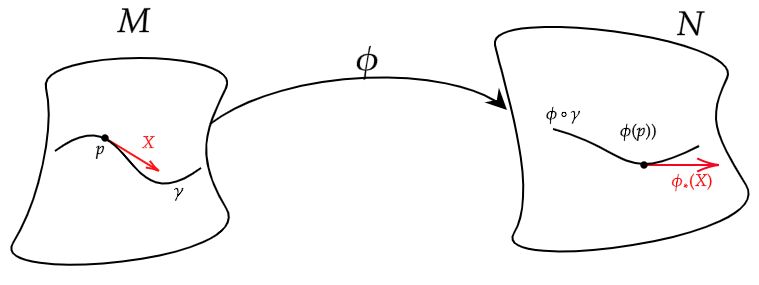
\includegraphics[scale=0.3]{Figs/pushcurve.png}
    % \caption{Caption}
    % \label{fig:my_label}
\end{figure}
\item \tb{local representation of push-forward:} with chart $(U,x)$ defined on $M$ and $(V,y)$ defined on $N$ such that $p\in U$ and $
\phi(p)\in V$, if $ X = X^i_{(x)} \bigg(\frac{\p}{\p x^i}\bigg)_p$, we have 
\begin{align*} 
    \begin{split}
       X_{\phi\circ\gamma,\phi(p)}(f)
       & = (f\circ(\phi\circ \gamma))'(0) \\
        & = (f\circ y^{-1}\circ y \circ  \phi \circ \gamma)'(0) \\
        & = (y^i\circ \phi \circ \gamma)'(0) \cdot \p_i \big( f\circ y^{-1}\big)\big|_{y(\phi(p))}\\
        & = (y^i\circ \phi \circ x^{-1} \circ x \circ \gamma)'(0) \cdot \p_i \big( f\circ y^{-1}\big)\big|_{y(\phi(p))}\\
        & = \p_j(y^i\circ \phi \circ x^{-1})|_{x(p)} X^j_{(x)} \bigg(\frac{\p}{\p y^i}\bigg)_{\phi(p)}
    \end{split}
\end{align*}

So $(\phi_*)_p$ has mapped 
\begin{align*}
    X = X^i_{(x)} \bigg(\frac{\p}{\p x^i}\bigg)_p \Rightarrow (\phi_*)_p(X)= \p_j(y^i\circ \phi \circ  x^{-1})|_{x(p)} X^j_{(x)} \bigg(\frac{\p}{\p y^i}\bigg)_{\phi(p)}
\end{align*} %$ X = X^i_{(y)} \bigg(\frac{\p}{\p y^i}\bigg)_p 
% (\phi_*)_p \cl & T_pM & \xrightarrow{\sim} & T_{\phi(p)}N\\
% & X & \mapsto & (\phi_*)_p(X) := X(-\circ \phi).

\end{itemize}
\item \tb{pull-back:}
Let $\phi\cl M \to N$ be a smooth map between smooth manifolds. The \tb{pull-back} of $\phi$ at $p\in M$ is the \tb{linear map}:
\bi{rrCl}
(\phi^*)_p \cl & T^*_{\phi(p)}N & \xrightarrow{\sim} & T^*_pM\\
& \omega & \mapsto & (\phi^*)_p(\omega),
\ei
where $(\phi^*)_p(\omega)$ is defined as
\bi{rrCl}
(\phi^*)_p(\omega) \cl & T_pM & \xrightarrow{\sim} & \R\\
& X & \mapsto & \omega((\phi_*)_p(X)),
\ei
\begin{itemize}
   \item \tb{one convention:} Given a smooth map $\phi\cl M \to N$, if $f\in \mathcal{C}^\infty (N)$, sometimes $f\circ \phi$ is often called the \tb{pull-back of $f$ along $\phi$.}
   \item \tb{local representation of pull-back:} with chart $(U,x)$ defined on $M$ and $(V,y)$ defined on $N$ such that $p\in U$ and $\phi(p)\in V$, if $ \omega = \omega_{k(y)} (\d y^k)_{\phi(p)}$, we then use dual basis:
\begin{align*}
    \omega((\phi_*)_p(\bigg(\frac{\p}{\p x^m}\bigg)_p))
    & =  \omega_{k(y)} (\d y^k)_{\phi(p)} \Big( \p_m(y^i\circ \phi \circ x^{-1})|_{x(p)}  \bigg(\frac{\p}{\p y^i}\bigg)_{\phi(p)} \Big)\\
    & =  \omega_{k(y)} \p_m(y^k\circ \phi \circ x^{-1})|_{x(p)} 
\end{align*}
So $(\phi^*)_p$ has mapped 
\begin{align*}
    \omega = \omega_{k(y)} (\d y^k)_{\phi(p)} \Rightarrow
    (\phi^*)_p(\omega) = \omega_{k(y)} \p_m(y^k\circ \phi \circ x^{-1})|_{x(p)}  (\d x^m)_{p}
\end{align*}
Note, here \cyan{$\omega_{k(y)}$ is the component at $\phi(p)$}!


\end{itemize}

\item \tb{discussion of push-forward and pull-back:}
\begin{itemize}
    \item In most cases, \tb{\magenta{vectors are pushed forward; covectors are pulled back.}} They are always well-defined and are \tb{$\Real$-linear maps}.
    \bse
\begin{tikzcd}
\mathcal{C}^\infty(M) \ar[dd,"X"] && \mathcal{C}^\infty(N) \ar[ll,"-\circ\phi"']\ar[ddll,"(\phi_*)_p(X)"]   && T_pM \ar[rr,"(\phi_*)_p"] \ar[ddrr,"(\phi^*)_p(\omega)"'] && T_{\phi(p)}N \ar[dd,"\omega"]\\
&& && &&\\
\R&& && && \R
\end{tikzcd}
\ese
\begin{itemize}[$\ast$]
    \item Generally speaking, \cyan{any tensor \tb{at one point}} can be push-forward and pull-back.
\end{itemize}
    \item If $\phi\cl M\to N$ is a \magenta{\tb{diffeomorphism}},  \magenta{\tb{by using $\phi^{-1}$}} then we can also \tb{\magenta{pull a vector $Y\in T_{\phi(p)}N$ back}} to a vector $(\phi^*)_p(Y)\in T_pM$, and \tb{\magenta{push a covector $\eta \in T^*_pM$ forward}} to a covector $(\phi_*)_p(\eta)\in T_{\phi(p)}^*N$:
\bi{rCl}
(\phi^*)_p(Y) & := & ((\phi^{-1})_*)_{\phi(p)}(Y)\\
(\phi_*)_p(\eta) & := & (({\phi^{-1}})^*)_{\phi(p)}(\eta).
\ei

\bse
\begin{tikzcd}
\mathcal{C}^\infty(M) \ar[rr,"-\circ\phi^{-1}"] \ar[ddrr,"(\phi^*)_p(Y)"'] && \mathcal{C}^\infty(N) \ar[dd,"Y"]    && T_pM \ar[dd,"\eta"']   &&& T_{\phi(p)}N \ar[lll,"((\phi^{-1})_*)_{\phi(p)}"'] \ar[ddlll,"(\phi_*)_p(\eta)"] \\
&& && &&\\
&& \R && \R && 
\end{tikzcd}
\ese
\item We have that \magenta{\tb{global push-forward for vector fields}}  needs  \magenta{\tb{diffeomorphism}}. However \magenta{\tb{global pull-back for covector fields}} is  still always well-defined.  See \cref{sec:tensorII} for more details.
\end{itemize}




\begin{figure}[H]
    \centering
    

\tikzset{every picture/.style={line width=0.75pt}} %set default line width to 0.75pt        

\begin{tikzpicture}[x=0.75pt,y=0.75pt,yscale=-1,xscale=1]
%uncomment if require: \path (0,300); %set diagram left start at 0, and has height of 300

%Shape: Polygon Curved [id:ds6554644297393142] 
\draw  [fill={rgb, 255:red, 80; green, 227; blue, 194 }  ,fill opacity=1 ] (82,84.5) .. controls (77.5,64.5) and (181.5,64.5) .. (172,84.5) .. controls (162.5,104.5) and (155.5,117.5) .. (172,144.5) .. controls (188.5,171.5) and (52.5,183) .. (65.5,162) .. controls (78.5,141) and (86.5,104.5) .. (82,84.5) -- cycle ;
%Shape: Polygon Curved [id:ds4762756981904337] 
\draw   (305,70.5) .. controls (300.5,50.5) and (430.5,67) .. (421,87) .. controls (411.5,107) and (414,113.5) .. (430.5,140.5) .. controls (447,167.5) and (301.5,185.5) .. (314.5,164.5) .. controls (327.5,143.5) and (309.5,90.5) .. (305,70.5) -- cycle ;
%Curve Lines [id:da7590416620497824] 
\draw    (162.5,110) .. controls (201.5,80.75) and (303.24,84.3) .. (329.62,105.35) ;
\draw [shift={(331.5,107)}, rotate = 224.37] [fill={rgb, 255:red, 0; green, 0; blue, 0 }  ][line width=0.08]  [draw opacity=0] (10.72,-5.15) -- (0,0) -- (10.72,5.15) -- (7.12,0) -- cycle    ;
%Shape: Polygon Curved [id:ds0987024053696337] 
\draw  [fill={rgb, 255:red, 80; green, 227; blue, 194 }  ,fill opacity=1 ] (351.5,93) .. controls (371.5,83) and (373.5,76.5) .. (386,93.5) .. controls (398.5,110.5) and (406.5,120.5) .. (392,138.5) .. controls (377.5,156.5) and (363,166.5) .. (343,136.5) .. controls (323,106.5) and (331.5,103) .. (351.5,93) -- cycle ;
%Straight Lines [id:da1504825094536959] 
\draw [color={rgb, 255:red, 242; green, 8; blue, 37 }  ,draw opacity=1 ]   (352.5,123.5) -- (363.32,93.38) ;
\draw [shift={(364,91.5)}, rotate = 109.77] [color={rgb, 255:red, 242; green, 8; blue, 37 }  ,draw opacity=1 ][line width=0.75]    (10.93,-3.29) .. controls (6.95,-1.4) and (3.31,-0.3) .. (0,0) .. controls (3.31,0.3) and (6.95,1.4) .. (10.93,3.29)   ;
%Straight Lines [id:da20796514882569928] 
\draw [color={rgb, 255:red, 23; green, 28; blue, 234 }  ,draw opacity=1 ]   (352.5,123.5) -- (379.79,107.03) ;
\draw [shift={(381.5,106)}, rotate = 148.89] [color={rgb, 255:red, 23; green, 28; blue, 234 }  ,draw opacity=1 ][line width=0.75]    (10.93,-3.29) .. controls (6.95,-1.4) and (3.31,-0.3) .. (0,0) .. controls (3.31,0.3) and (6.95,1.4) .. (10.93,3.29)   ;
%Straight Lines [id:da7934594673027966] 
\draw [color={rgb, 255:red, 251; green, 21; blue, 21 }  ,draw opacity=1 ]   (111.5,107.5) -- (136.46,86.78) ;
\draw [shift={(138,85.5)}, rotate = 140.3] [color={rgb, 255:red, 251; green, 21; blue, 21 }  ,draw opacity=1 ][line width=0.75]    (10.93,-3.29) .. controls (6.95,-1.4) and (3.31,-0.3) .. (0,0) .. controls (3.31,0.3) and (6.95,1.4) .. (10.93,3.29)   ;
%Straight Lines [id:da3555160209717785] 
\draw [color={rgb, 255:red, 12; green, 25; blue, 242 }  ,draw opacity=1 ]   (119.5,144) -- (149.05,150.57) ;
\draw [shift={(151,151)}, rotate = 192.53] [color={rgb, 255:red, 12; green, 25; blue, 242 }  ,draw opacity=1 ][line width=0.75]    (10.93,-3.29) .. controls (6.95,-1.4) and (3.31,-0.3) .. (0,0) .. controls (3.31,0.3) and (6.95,1.4) .. (10.93,3.29)   ;
%Straight Lines [id:da0025080390592564505] 
\draw    (111.5,107.5) ;
\draw [shift={(111.5,107.5)}, rotate = 0] [color={rgb, 255:red, 0; green, 0; blue, 0 }  ][fill={rgb, 255:red, 0; green, 0; blue, 0 }  ][line width=0.75]      (0, 0) circle [x radius= 1.34, y radius= 1.34]   ;
%Straight Lines [id:da9067359738721119] 
\draw    (119.5,144) ;
\draw [shift={(119.5,144)}, rotate = 0] [color={rgb, 255:red, 0; green, 0; blue, 0 }  ][fill={rgb, 255:red, 0; green, 0; blue, 0 }  ][line width=0.75]      (0, 0) circle [x radius= 1.34, y radius= 1.34]   ;
%Straight Lines [id:da9190854195792948] 
\draw    (352.5,123.5) ;
\draw [shift={(352.5,123.5)}, rotate = 0] [color={rgb, 255:red, 0; green, 0; blue, 0 }  ][fill={rgb, 255:red, 0; green, 0; blue, 0 }  ][line width=0.75]      (0, 0) circle [x radius= 1.34, y radius= 1.34]   ;

% Text Node
\draw (238.5,69.4) node [anchor=north west][inner sep=0.75pt]    {$h$};
% Text Node
\draw (97.5,103.9) node [anchor=north west][inner sep=0.75pt]    {$p$};
% Text Node
\draw (107.5,140.9) node [anchor=north west][inner sep=0.75pt]    {$q$};
% Text Node
\draw (342.5,128.9) node [anchor=north west][inner sep=0.75pt]  [font=\tiny]  {$h( p) =h( q)$};
% Text Node
\draw (115.5,49.9) node [anchor=north west][inner sep=0.75pt]    {$M$};
% Text Node
\draw (395,51.4) node [anchor=north west][inner sep=0.75pt]    {$N$};
% Text Node
\draw (342,155.9) node [anchor=north west][inner sep=0.75pt]  [font=\tiny]  {$h( M)$};


\end{tikzpicture}

    % \caption{Caption}
    % \label{fig:my_label}
\end{figure}

\item \tb{immersion:} A smooth map $\phi\cl M \to N$ is said to be an \tb{immersion} of $M$ into $N$ if the differential
\bse
d \phi_p\cl T_pM\xrightarrow{\sim}T_{\phi(p)}N
\ese
is \tb{injective}, for all $p\in M$. The manifold $M$ is said to be an \tb{immersed submanifold} of $N$.

\begin{itemize}
    \item  For $\phi\cl M\to N$ to be an immersion, we must have $\dim M \leq \dim N$. 
    \begin{figure}[H]
    \centering
    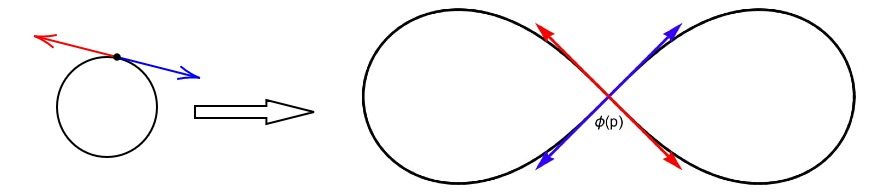
\includegraphics[scale=0.3]{Figs/embed.jpg}
    \caption{Immersion}
    \label{fig:immersion}
\end{figure}
\item Example: The map $\phi$ is not injective. However, the maps $(\phi_*)_p$ and $(\phi_*)_q$ are both injective. Hence, the map $\phi$ is immersion.
\end{itemize}
\item \tb{submersion:} A smooth map $\phi: M \rightarrow N$ is a \tb{submersion} at a point $p \in M$ if its differential
\begin{align*}
d \phi_p: T_p M \xrightarrow{\sim} T_{\phi(p)} N
\end{align*}
is a \tb{surjective} linear map. A differentiable map $\phi$ that is a \tb{submersion} at each point $p \in M$ is called a submersion. 
\begin{itemize}
\item Equivalently, $\phi$ is a submersion if its differential $d \phi_p$ has constant rank equal to the dimension of $N$.
    \item \tb{regular and critical point:} In the case of submersion, $p$ is called a \tb{regular point} of the map $\phi$, otherwise, $p$ is a \tb{critical point}. A point $q \in N$ is a regular value of $\phi$ if all points $p$ in the preimage $\phi^{-1}(q)$ are regular points. 
    \item For $\phi\cl M\to N$ to be an submersion, we must have $\dim M \geq \dim N$. 
\end{itemize}


\item \tb{immersion vs. submersion:}{\tiny
\tb{The Rank Theorem} may provide some insight into these concepts. 
Suppose $M$ and $N$ are smooth manifolds of dimensions $m$ and $n$, respectively, and $F: M \rightarrow N$ is a smooth map with constant rank $r$. For each $p \in M$ there exist smooth charts $(U, \varphi)$ for $M$ centered at $p$ and $(V, \psi)$ for $N$ centered at $F(p)$ such that $F(U) \subseteq V$, in which $F$ has a coordinate representation of the form
\begin{align*}
\hat{F}\left(x^1, \ldots, x^r, x^{r+1}, \ldots, x^m\right)=\left(x^1, \ldots, x^r, 0, \ldots, 0\right) .
\end{align*}
In particular, if $F$ is a smooth \tb{submersion}, this becomes
\begin{align*}
\hat{F}\left(x^1, \ldots, x^n, x^{n+1}, \ldots, x^m\right)=\left(x^1, \ldots, x^n\right),
\end{align*}
and if $F$ is a smooth \tb{immersion}, it is
\begin{align*}
\hat{F}\left(x^1, \ldots, x^m\right)=\left(x^1, \ldots, x^m, 0, \ldots, 0\right) .
\end{align*}}
\begin{itemize}
    \item A \tb{submersion} locally looks like a \tb{projection} $\mathbb{R}^n \times \mathbb{R}^{m-n} \rightarrow \mathbb{R}^n$, 
    \item An \tb{immersion} locally looks like an \tb{inclusion} $\mathbb{R}^m \rightarrow \mathbb{R}^m \times \mathbb{R}^{n-m}$.
\end{itemize}


\item \tb{embedding:}
A smooth map $\phi\cl M \to N$ is said to be a \tb{(smooth) embedding} of $M$ into $N$ if
\begin{itemize}
\item $\phi\cl M\to N$ is an \tb{immersion};
\item $M \cong_{\mathrm{top}}\phi(M)\se N$, where $\phi(M)$ carries the \tb{subset topology} inherited from $N$.
\end{itemize}
The manifold $M$ is said to be an \tb{embedded submanifold} of $N$.

\begin{figure}[H]
    \centering
\tikzset{every picture/.style={line width=0.75pt}} %set default line width to 0.75pt        

\begin{tikzpicture}[x=0.75pt,y=0.75pt,yscale=-0.7,xscale=0.7]
%uncomment if require: \path (0,300); %set diagram left start at 0, and has height of 300

%Shape: Circle [id:dp9494255109047431] 
\draw   (106.5,147.5) .. controls (106.5,133.69) and (117.69,122.5) .. (131.5,122.5) .. controls (145.31,122.5) and (156.5,133.69) .. (156.5,147.5) .. controls (156.5,161.31) and (145.31,172.5) .. (131.5,172.5) .. controls (117.69,172.5) and (106.5,161.31) .. (106.5,147.5) -- cycle ;
%Right Arrow [id:dp022853372326593346] 
\draw   (175.5,147) -- (211.2,147) -- (211.2,144) -- (235,150) -- (211.2,156) -- (211.2,153) -- (175.5,153) -- cycle ;
%Shape: Polygon Curved [id:ds24072134862856998] 
\draw   (263,115) .. controls (283,105) and (373,95) .. (353,115) .. controls (333,135) and (333,145) .. (353,175) .. controls (373,205) and (283,205) .. (263,175) .. controls (243,145) and (243,125) .. (263,115) -- cycle ;
%Straight Lines [id:da5516422197978352] 
\draw [color={rgb, 255:red, 8; green, 5; blue, 246 }  ,draw opacity=1 ]   (136.5,122.5) -- (176.06,132.51) ;
\draw [shift={(178,133)}, rotate = 194.2] [color={rgb, 255:red, 8; green, 5; blue, 246 }  ,draw opacity=1 ][line width=0.75]    (10.93,-3.29) .. controls (6.95,-1.4) and (3.31,-0.3) .. (0,0) .. controls (3.31,0.3) and (6.95,1.4) .. (10.93,3.29)   ;
%Straight Lines [id:da3259240284174276] 
\draw [color={rgb, 255:red, 247; green, 6; blue, 6 }  ,draw opacity=1 ]   (136.5,122.5) -- (96.94,112.49) ;
\draw [shift={(95,112)}, rotate = 14.2] [color={rgb, 255:red, 247; green, 6; blue, 6 }  ,draw opacity=1 ][line width=0.75]    (10.93,-3.29) .. controls (6.95,-1.4) and (3.31,-0.3) .. (0,0) .. controls (3.31,0.3) and (6.95,1.4) .. (10.93,3.29)   ;
%Straight Lines [id:da9180209773509527] 
\draw    (136.5,122.5) ;
\draw [shift={(136.5,122.5)}, rotate = 0] [color={rgb, 255:red, 0; green, 0; blue, 0 }  ][fill={rgb, 255:red, 0; green, 0; blue, 0 }  ][line width=0.75]      (0, 0) circle [x radius= 1.34, y radius= 1.34]   ;
%Straight Lines [id:da7402863783783087] 
\draw    (248.5,144) ;
\draw [shift={(248.5,144)}, rotate = 0] [color={rgb, 255:red, 0; green, 0; blue, 0 }  ][fill={rgb, 255:red, 0; green, 0; blue, 0 }  ][line width=0.75]      (0, 0) circle [x radius= 1.34, y radius= 1.34]   ;
%Straight Lines [id:da7685474275182997] 
\draw [color={rgb, 255:red, 8; green, 5; blue, 246 }  ,draw opacity=1 ]   (248.5,144.5) -- (260.77,183.42) ;
\draw [shift={(261.37,185.33)}, rotate = 252.51] [color={rgb, 255:red, 8; green, 5; blue, 246 }  ,draw opacity=1 ][line width=0.75]    (10.93,-3.29) .. controls (6.95,-1.4) and (3.31,-0.3) .. (0,0) .. controls (3.31,0.3) and (6.95,1.4) .. (10.93,3.29)   ;
%Straight Lines [id:da21214128154850176] 
\draw [color={rgb, 255:red, 247; green, 6; blue, 6 }  ,draw opacity=1 ]   (248.5,144.5) -- (236.23,105.58) ;
\draw [shift={(235.63,103.67)}, rotate = 72.51] [color={rgb, 255:red, 247; green, 6; blue, 6 }  ,draw opacity=1 ][line width=0.75]    (10.93,-3.29) .. controls (6.95,-1.4) and (3.31,-0.3) .. (0,0) .. controls (3.31,0.3) and (6.95,1.4) .. (10.93,3.29)   ;
\end{tikzpicture}
    \caption{Embedding}
    \label{fig:Embedding}
\end{figure}

\begin{itemize}
    \item embedding is called \tb{extrinsic view}, while in this course we mainly focus on \tb{intrinsic view} where the tangent space are defined without using any ambient space.
    \item Example: See the figure.
\end{itemize}
\item \tb{Whitney's theorem:}
Any smooth manifold $M$ can be
\begin{enumerate}
\item embedded in $\R^{2\dim M}$;
\item immersed in $\R^{2\dim M-1}$.
\end{enumerate}
\begin{itemize}
    \item Whitney's theorem states that \tb{extrinsic view} and \tb{intrinsic view}  are essentially the same.
    \item Whitney's theorem states the loosest bound.
    \item Example: The Klein bottle can be embedded in $\R^4$ but not in $\R^3$. It can, however, be immersed in $\R^3$. The intersection is still a issue in  $\R^3$, similar to the intersection issue in \cref{fig:Embedding}.
    \item \tb{improved version:} Any smooth manifold can be immersed in $\R^{2\dim M-a(\dim M)}$, where $a(n)$ is the number of $1$s in a binary expansion of $n\in \N$. If $\dim M = 3$, then as  $3_{10}=(1\times 2^1+1\times 2^0)_{10}=11_2$, we have $a(\dim M)=2$, 
\end{itemize}


\item \tb{tangent bundle:} Given a smooth manifold $M$, the \tb{tangent bundle} of $M$ is the \tb{disjoint union} of all the tangent spaces to $M$, i.e.\
\bse
TM :=\coprod_{p\in M}T_pM,
\ese
equipped with the \tb{canonical projection map}
\bi{rrCl}
\pi \cl & TM & \to & M\\
& X & \mapsto & p,
\ei
where $p$ is the \tb{unique} $p\in M$ such that $X\in T_pM$.
\begin{itemize}
    \item $T_pM$ and  $T_qM$ are totally different vector spaces if $p\ne q$ (\tb{disjoint union} is therefore guaranteed). To define a smooth change between vectors from those tangent spaces at each point, we introduce the tangent bundle and then the smooth change is defined as the \tb{smooth section} between base manifold to total manifold.
    \begin{figure}[H]
    \begin{center}
        \btik[scale=1,point/.style = {draw, circle, fill=black, inner sep=0.7pt}]
            \def\rad{2cm}
            \coordinate (O) at (0,0); 
            \coordinate (N) at (0.7,1.5); 
            \coordinate (Q) at (1,-1.5);
            %
            \filldraw[ball color=white] (O) circle [radius=\rad];
            \draw[dashed] (\rad,0) arc [start angle=0,end angle=180,x radius=\rad,y radius=5mm];
            \draw (\rad,0) arc [start angle=0,end angle=-180,x radius=\rad,y radius=5mm];
            \begin{scope}[xslant=-1,yshift=40,xshift=56]
                \filldraw[fill=blue!10,opacity=0.8] (-1,0.6) -- (1.2,1) -- (1.2,-0.6) -- (-1,-1.2) -- cycle;
            \end{scope}
            \begin{scope}[xslant=0.5,yslant=0.5,yshift=-65,xshift=47]
                \filldraw[fill=red!10,opacity=0.8] (-1,1) -- (1,0.6) -- (1,-1) -- (-0.8,-0.8) -- cycle;
            \end{scope}
            \node[ultra thick, point] at (Q) {};
            \node[ultra thick, point] at (N) {};
            \node at (0.9,1.7) {{$p$}};
            \node at (1,-1.8) {{$q$}};
            \node at (-1.8,1.6) {$\calM$};
            \draw[very thick, ->] (0.7,1.5) -- (2,0.8);
            \draw[very thick, ->] (0.7,1.5) -- (1,0.9);
            \draw[very thick, color = blue,  ->] (1,-1.5) -- (2,-0.8);
            \etik
        % \caption{Tangent planes at two points $p,q$ on the sphere $\mathcal{M}$. The two velocity vectors at $p$ (black arrows) can be added because they live in the same tangent space, but it does not make sense to add one of them to the velocity at $q$ blue arrow.}
        % \label{fig:Tangent}
    \end{center}
\end{figure}
\item Currently the $TM$ is only a \tb{set bundle}. We need assign it a manifold structure and show it is indeed have the locally trivial property to make it a fibre bundle.
\item Later we will define \tb{connection} to numerically compare the vectors from different tangent space. Currently, we can only talk about the smoothness.
\end{itemize}
\begin{figure}
    \centering
    

% Pattern Info
 
\tikzset{
pattern size/.store in=\mcSize, 
pattern size = 5pt,
pattern thickness/.store in=\mcThickness, 
pattern thickness = 0.3pt,
pattern radius/.store in=\mcRadius, 
pattern radius = 1pt}
\makeatletter
\pgfutil@ifundefined{pgf@pattern@name@_f6dl8ivph}{
\pgfdeclarepatternformonly[\mcThickness,\mcSize]{_f6dl8ivph}
{\pgfqpoint{0pt}{-\mcThickness}}
{\pgfpoint{\mcSize}{\mcSize}}
{\pgfpoint{\mcSize}{\mcSize}}
{
\pgfsetcolor{\tikz@pattern@color}
\pgfsetlinewidth{\mcThickness}
\pgfpathmoveto{\pgfqpoint{0pt}{\mcSize}}
\pgfpathlineto{\pgfpoint{\mcSize+\mcThickness}{-\mcThickness}}
\pgfusepath{stroke}
}}
\makeatother
\tikzset{every picture/.style={line width=0.75pt}} %set default line width to 0.75pt        

\begin{tikzpicture}[x=0.75pt,y=0.75pt,yscale=-1,xscale=1]
%uncomment if require: \path (0,300); %set diagram left start at 0, and has height of 300

%Curve Lines [id:da740834057307419] 
\draw    (234.5,181) .. controls (274.5,151) and (352,161) .. (383.5,181) ;
%Straight Lines [id:da8676298116860939] 
\draw    (331,105) -- (315,207) ;
%Straight Lines [id:da8405278719416394] 
\draw    (288,103) -- (287.5,205.5) ;
%Straight Lines [id:da35811105895250783] 
\draw    (249.5,105.5) -- (269,209.5) ;
%Straight Lines [id:da2074582721665108] 
\draw    (261.5,168) ;
\draw [shift={(261.5,168)}, rotate = 0] [color={rgb, 255:red, 0; green, 0; blue, 0 }  ][fill={rgb, 255:red, 0; green, 0; blue, 0 }  ][line width=0.75]      (0, 0) circle [x radius= 1.34, y radius= 1.34]   ;
%Straight Lines [id:da16663398510947114] 
\draw    (288,162.5) ;
\draw [shift={(288,162.5)}, rotate = 0] [color={rgb, 255:red, 0; green, 0; blue, 0 }  ][fill={rgb, 255:red, 0; green, 0; blue, 0 }  ][line width=0.75]      (0, 0) circle [x radius= 1.34, y radius= 1.34]   ;
%Straight Lines [id:da3077016856882331] 
\draw    (321.5,163) ;
\draw [shift={(321.5,163)}, rotate = 0] [color={rgb, 255:red, 0; green, 0; blue, 0 }  ][fill={rgb, 255:red, 0; green, 0; blue, 0 }  ][line width=0.75]      (0, 0) circle [x radius= 1.34, y radius= 1.34]   ;
%Straight Lines [id:da13818097086187442] 
\draw [color={rgb, 255:red, 242; green, 6; blue, 6 }  ,draw opacity=1 ]   (321.5,163) -- (327.16,130.47) ;
\draw [shift={(327.5,128.5)}, rotate = 99.87] [color={rgb, 255:red, 242; green, 6; blue, 6 }  ,draw opacity=1 ][line width=0.75]    (4.37,-1.32) .. controls (2.78,-0.56) and (1.32,-0.12) .. (0,0) .. controls (1.32,0.12) and (2.78,0.56) .. (4.37,1.32)   ;
%Shape: Polygon [id:ds5687788087915358] 
\draw  [draw opacity=0][pattern=_f6dl8ivph,pattern size=6pt,pattern thickness=0.75pt,pattern radius=0pt, pattern color={rgb, 255:red, 184; green, 233; blue, 134}][dash pattern={on 4.5pt off 4.5pt}] (314,87.5) -- (379.5,88.5) -- (346.5,215) -- (305,211.5) -- (310,148) -- cycle ;
%Curve Lines [id:da29376603032045256] 
\draw [color={rgb, 255:red, 144; green, 19; blue, 254 }  ,draw opacity=1 ]   (327.5,128.5) .. controls (315.8,136.79) and (307.43,141.75) .. (320.46,161.45) ;
\draw [shift={(321.5,163)}, rotate = 235.38] [color={rgb, 255:red, 144; green, 19; blue, 254 }  ,draw opacity=1 ][line width=0.75]    (4.37,-1.32) .. controls (2.78,-0.56) and (1.32,-0.12) .. (0,0) .. controls (1.32,0.12) and (2.78,0.56) .. (4.37,1.32)   ;
%Curve Lines [id:da6581115255622392] 
\draw [color={rgb, 255:red, 5; green, 206; blue, 249 }  ,draw opacity=1 ]   (310,162) .. controls (328,164) and (332.5,163.5) .. (358.5,169.5) ;

% Text Node
\draw (323.5,166.4) node [anchor=north west][inner sep=0.75pt]  [font=\tiny]  {$p$};
% Text Node
\draw (324,100.4) node [anchor=north west][inner sep=0.75pt]  [font=\tiny]  {$T_{p} M$};
% Text Node
\draw (333,127.4) node [anchor=north west][inner sep=0.75pt]  [font=\tiny,color={rgb, 255:red, 247; green, 5; blue, 5 }  ,opacity=1 ]  {$X\in T_{p} M$};
% Text Node
\draw (344,169.4) node [anchor=north west][inner sep=0.75pt]  [font=\tiny,color={rgb, 255:red, 5; green, 238; blue, 248 }  ,opacity=1 ]  {$U$};
% Text Node
\draw (305.5,139.4) node [anchor=north west][inner sep=0.75pt]  [font=\tiny,color={rgb, 255:red, 144; green, 19; blue, 254 }  ,opacity=1 ]  {$\pi $};
% Text Node
\draw (359.5,104.9) node [anchor=north west][inner sep=0.75pt]  [font=\tiny,color={rgb, 255:red, 74; green, 134; blue, 14 }  ,opacity=0.98 ]  {$\pi ^{-1}( U)$};
% Text Node
\draw (382.5,174.9) node [anchor=north west][inner sep=0.75pt]  [font=\tiny]  {$M$};


\end{tikzpicture}
\end{figure}
\item \tb{equip $TM$ with the structure of a smooth manifold:} Let $\mathscr{A}_M$ be a smooth atlas on $M$ and let $(U,x)\in \mathscr{A}_M$. If $X\in \preim_\pi(U)\se TM$, then $X\in T_{\pi(X)}M$, by definition of $\pi$. Moreover, since $\pi(X)\in U$, we can expand $X$ in terms of the basis induced by the chart $(U,x)$:
\bse
X = X^a \tvb{x}{a}{\pi(X)},
\ese
where $X^1,\ldots,X^{\dim M}\in \R$. We can then define the \tb{map}
\bi{rrCl}
\xi \cl & \preim_\pi(U) & \to & x(U) \times \R^{\dim M} \cong_{\mathrm{set}}\R^{2\dim M}\\
& X & \mapsto & (x(\pi(X)),X^1,\ldots,X^{\dim M}).
\ei
We then equip $TM$ with  the \tb{initial topology}, we claim that \tb{the pair $(\preim_\pi(U),\xi)$ is a chart} on $TM$ and 
\bse
\mathscr{A}_{TM} := \{(\preim_\pi(U),\xi)\mid (U,x) \in \mathscr{A}_M\}
\ese
is a \tb{smooth atlas} on $TM$. 
\begin{itemize}
\item Note that, from its definition, it is clear that $\xi$ is a bijection. We can  show that $(\preim_\pi(U),\xi)$ is a \tb{chart} but we omit the details.
    \item  We also can show that $\mathscr{A}_{TM}$ is a \tb{smooth atlas}: any two charts $(\preim_\pi(U),\xi), (\preim_\pi(\widetilde U),\widetilde \xi)\in\mathscr{A}_{TM}$ are $\mathcal{C}^\infty$-compatible.
    \item The \tb{locally trivial} property then follows immediately: the required homeomorphism map is $x^{-1}\circ \proj_1\circ \xi: \preim_\pi(U)\to U\times \R^{\dim M}$:
    \bse
\begin{tikzcd}
  && \preim_\pi(U) \ar[dd,"\pi"']   &&& U\times \R^{\dim M} \ar[lll,"x^{-1}\circ \proj_1\circ \xi"'] \ar[ddlll,"\proj_1"] \\
&& && &&\\
&& U &&  && 
\end{tikzcd}
\ese
\end{itemize}







\item \tb{cotangent bundle:}  Similarly, one can construct the \tb{cotangent bundle} $T^*M$ to $M$ by defining
\bse
T^*M := \coprod_{p\in M} T^*_pM
\ese
and going through the above again, using the dual basis $\{(\d x^a)_p\}$ instead of $\{\tvb{x}{a}{p}\}$.


\item \tb{$(r,s)$ tensor bundle:} Similarly, $(r,s)$ tensor bundle of $M$ is defined as
\bse
T^r_sM := \coprod_{p\in M}(T^r_s)_pM.
\ese

\end{enumerate}


\section{Tensor Field and Tensor Space Theory II: Over A Ring}\label{sec:tensorII}

A summary:
\begin{itemize}[$\blacktriangleright$]
\item Following from the bundles from last \cref{sec:cotangent}, we construct \tb{vector, covector, and tensor fields} using \tb{smooth sections}.
\item The \magenta{\tb{global}} push-forward for \tb{vector fields}  needs additional condition  \tb{diffeomorphism}. However \magenta{\tb{global}} pull-back for \tb{covector fields} is  still always possible.
\item We show vector fields have \tb{module properties} with the ring $\calC^\infty(M)$ and then formally introduce \tb{rings and modules over a ring}. 
\item We show \tb{bases for modules} and when it is possible. \tb{Module $R$-linear map} and \tb{module isomorphism} are also defined.
\item From modules, we show applications like constructing \tb{covector fields} and \tb{tensor fields} using $\calC^\infty(M)$ multilinear map.
\end{itemize}


\begin{enumerate}
    \item \orange{\tb{vector field (equivalent definition I):}}
    Let $M$ be a smooth manifold, and let $TM\xrightarrow{\,\pi\,}M$ be its tangent bundle. A \tb{vector field} on $M$ is a \tb{\cyan{smooth}\footnote{In this note, we only consider smooth sections as vector fields.} section} of the tangent bundle, i.e.\ a smooth map $\sigma\cl M \to TM$ such that $\pi \circ \sigma = \id_M$.
\bse
\begin{tikzcd}
TM \ar[dd,shift left,"\pi"] \\
\\
M \ar[uu,shift left,"\sigma"]
\end{tikzcd}
\ese

\begin{itemize} 
    \item \tb{notation:} We denote the \tb{set of all vector fields on $M$} by $\Gamma(TM)$, i.e.\
\bse
\Gamma(TM) := \{\sigma \cl M \to TM \mid \sigma \text{ is smooth and }\pi\circ\sigma=\id_M\}.
\ese
\item \orange{\tb{vector field equivalent definition II:}}  A vector field $\sigma$ on $M$ is a \tb{derivation} on the algebra $\mathcal{C}^\infty(M)$, i.e.\ an \tb{$\R$-linear map}
\bse
\sigma\cl \mathcal{C}^\infty(M) \xrightarrow{\sim} \mathcal{C}^\infty(M)
\ese
satisfying the \tb{Leibniz rule} (\gls{wrt} \cyan{dot multiplication} (i.e. pointwise multiplication) on algebra $\mathcal{C}^\infty(M)$) 
\bse
\sigma (fg) = g\, \sigma(f) + f \, \sigma(g).
\ese
\begin{itemize}[$\ast$]
    \item  This definition is similar to \tb{tangent space equivalent definition III} in \cref{sec:tangent}, where we use bimodule there. Here, we define the derivation globally from $ \mathcal{C}^\infty(M) \xrightarrow{\sim} \mathcal{C}^\infty(M)$.
    \item Later we will see we can also view vector field as $\calC^{\infty}(M)$-linear map from $\Gamma(T^*M)$ to $\mathcal{C}^\infty(M)$. Don't be confused. Even we can map function  $f$ to covector field $\d f$, $\calC^{\infty}(M)$-linear map means $g(p)\d_pf$ \tb{not}  $g(p)f(p)$ pointwisely.
\end{itemize}
\item Example: \tb{vector fields locally from chart:} Let $(U,x)$ be a chart on $M$. For each $1\leq a \leq \dim M$, the map
\bi{rrCl}
\frac{\partial}{\partial x^a} \cl & U & \to & TU\\
& p &\mapsto &\tvb{x}{a}{p}
\ei
is a vector field on the \tb{submanifold $U$}. We can also think of this as a \tb{derivation}, i.e., \tb{$\R$-linear map}, over the algebra $\mathcal{C}^\infty(U)$:
\bi{rrCl}
\frac{\partial}{\partial x^a} \cl & \mathcal{C}^\infty(U) & \xrightarrow{\sim} & \mathcal{C}^\infty(U)\\
& f & \mapsto & \frac{\partial}{\partial x^a}(f) = \partial_a(f\circ x^{-1}). 
\ei
By abuse of notation, one usually denotes the right hand side  as $\partial_a f$.
\end{itemize}

\item \purple{\tb{covector field (equivalent definition I):}} Analogously,  we could define the \tb{covector fields} as smooth sections on $T^*M$. 
\bse
\begin{tikzcd}
T^*M \ar[dd,shift left,"\pi"] \\
\\
M \ar[uu,shift left,"\omega"]
\end{tikzcd}
\ese

\begin{itemize} 
    \item \tb{notation:} We denote the \tb{set of all covector fields on $M$} by $\Gamma(TM)$, i.e.\
\bse
\Gamma(T^*M) := \{\omega \cl M \to T^*M \mid \omega \text{ is smooth and }\pi\circ\omega=\id_M\}.
\ese
\item Example I: \tb{vector fields locally from chart:} Let $(U,x)$ be a chart on $M$. For each $1\leq a \leq \dim M$, the map, the $\d x^{a_i}$ appearing above are the covector fields (i.e. called differentiable $1$-forms in \cref{sec:grass}) on the \tb{submanifold $U$}
\bi{rrCl}
\d x^{a}  \cl & U & \to & T^*U\\
& p &\mapsto &\d_px^{a}
\ei
\item Example II: \tb{vector fields from smooth function:} More generally, we have that for $f\in \calC^\infty(M)$, $\d f$ is a covector field.

\end{itemize}

\item \tb{tensor field (equivalent definition I):} Analogously,  we define the \tb{$(r,s)$ tensor fields} as smooth sections on \tb{$(r,s)$ tensor bundle} $T^r_sM$. We denote the set of all $(r,s)$ tensor fields on $M$ by $\Gamma(T^r_sM)$.
% \bse
% \begin{tikzcd}
% T^*M \ar[dd,shift left,"\pi"] \\
% \\
% M \ar[uu,shift left,"\omega"]
% \end{tikzcd}
% \ese

% \begin{itemize} 
%     \item \tb{notation:} We denote the \tb{set of all covector fields on $M$} by $\Gamma(TM)$\index{$\Gamma(T^*M)$}, i.e.\
% \bse
% \Gamma(TM) := \{\omega \cl M \to T^*M \mid \omega \text{ is smooth and }\pi\circ\omega=\id_M\}.
% \ese
% \end{itemize}

\item \tb{push-forward pointwisely:}
Let $\phi\cl M \to N$ be smooth. The \tb{push-forward} $\phi_*$ is defined as
\bi{rrCl}
\phi_*\cl & TM & \to & TN\\
& X &\mapsto & (\phi_*)_{\pi(X)}(X).
\ei
\begin{itemize}
\item Recall that, given a smooth map $\phi\cl M \to N$, \green{the push-forward $(\phi_*)_p$ is a linear map that takes in a tangent vector in $T_pM$ and outputs a tangent vector in $T_{\phi(p)}N$.} 
    \item Any vector $X\in TM$ must belong to $T_pM$ for some $p=\pi(X)\in M$. The map $\phi_*$ takes one vector $X\in TM$ and applies the push-forward at the ``right'' point, producing a vector in $TN$.
   \item \orange{\tb{compositions of push-forward:}} We have  $(g \circ f)_*=g_* \circ f_*$.
   
{\tiny Roughly speaking, we need the following \tb{chain rule} to prove it. More strictly, we need a local representation. But here I just show the $R^n$ case with $d$ being the traditional derivative.
$$(g\circ f)_*(X|_a)=(d (g\circ f)(a)(X|_a))_{(g\circ f)(a)}=\underbrace{(d g(f(a))_{g(f(a))}}_{g_*}) ( \underbrace{d f(a))_{f(a)}}_{f_*} )(X|_a)
$$}
\end{itemize}

\item \tb{pull-back pointwisely:} One can similarly define \tb{pull-back} $\phi^*$ where \tb{at each point $p\in M$}, where $(\phi^*)_p$ is defined as in \cref{sec:cotangent}. 
\begin{itemize}
    \item Better \tb{not} to think $\phi^*$ as a map from $T^*N \to T^*M$. It is not a map pointwise at each point in $N$. We first \green{select one point $p\in M$, and look at covector space $T^*_{\phi(p)}N$ at $\phi(p)\in N$. A covector space  $T^*_pM$ at $p\in M$ is then constructed.} 
    \item \orange{\tb{compositions of pull-back:}} We have  $(g \circ f)^*=g^* \circ f^*$.
\end{itemize}

\item \tb{global push-forward for vector fields:} We now construct a map $\Phi_*\cl\Gamma(TM)\to\Gamma(TN)$ that allows us to push vector fields on $M$ forward to vector fields on $N$.  Assume $\phi\cl M \to N$ is a \magenta{\tb{diffeomorphism}}.
\bse
\begin{tikzcd}
TM \ar[rr,"\phi_*"] && TN \\
\\
M \ar[uu,"\sigma"] \ar[rr,"\phi"] && N \ar[uu,"\Phi_*(\sigma)"']
\end{tikzcd}
\ese
If $\sigma \in \Gamma(TM)$, we can define the \tb{push-forward} $\Phi_*(\sigma)\in \Gamma(TN)$ as
\bse
\Phi_*(\sigma) := \phi_*\circ\sigma\circ\phi^{-1}.
\ese

\begin{itemize}
\item Do not be confused here. We still \green{push-forward tangent space at $p$ on manifold $M$ to tangent space at $\phi(p)$ on manifold $N$.} The above diagram is just for beauty.
    \item Why we need \magenta{\tb{diffeomorphism}}? See the figure.
        \begin{itemize}[$\ast$]
    \item The map $\phi$ may fail to be injective.
    \item The map $\phi$ may fail to be surjective. 
\end{itemize}
Both issues will make the push-forwarded vector field on $N$ not well-defined.
\begin{figure}[H]
    \centering
\tikzset{every picture/.style={line width=0.75pt}} %set default line width to 0.75pt        

\begin{tikzpicture}[x=0.75pt,y=0.75pt,yscale=-1,xscale=1]
%uncomment if require: \path (0,300); %set diagram left start at 0, and has height of 300

%Shape: Polygon Curved [id:ds6554644297393142] 
\draw  [fill={rgb, 255:red, 80; green, 227; blue, 194 }  ,fill opacity=1 ] (82,84.5) .. controls (77.5,64.5) and (181.5,64.5) .. (172,84.5) .. controls (162.5,104.5) and (155.5,117.5) .. (172,144.5) .. controls (188.5,171.5) and (52.5,183) .. (65.5,162) .. controls (78.5,141) and (86.5,104.5) .. (82,84.5) -- cycle ;
%Shape: Polygon Curved [id:ds4762756981904337] 
\draw   (305,70.5) .. controls (300.5,50.5) and (430.5,67) .. (421,87) .. controls (411.5,107) and (414,113.5) .. (430.5,140.5) .. controls (447,167.5) and (301.5,185.5) .. (314.5,164.5) .. controls (327.5,143.5) and (309.5,90.5) .. (305,70.5) -- cycle ;
%Curve Lines [id:da7590416620497824] 
\draw    (162.5,110) .. controls (201.5,80.75) and (303.24,84.3) .. (329.62,105.35) ;
\draw [shift={(331.5,107)}, rotate = 224.37] [fill={rgb, 255:red, 0; green, 0; blue, 0 }  ][line width=0.08]  [draw opacity=0] (10.72,-5.15) -- (0,0) -- (10.72,5.15) -- (7.12,0) -- cycle    ;
%Shape: Polygon Curved [id:ds0987024053696337] 
\draw  [fill={rgb, 255:red, 80; green, 227; blue, 194 }  ,fill opacity=1 ] (351.5,93) .. controls (371.5,83) and (373.5,76.5) .. (386,93.5) .. controls (398.5,110.5) and (406.5,120.5) .. (392,138.5) .. controls (377.5,156.5) and (363,166.5) .. (343,136.5) .. controls (323,106.5) and (331.5,103) .. (351.5,93) -- cycle ;
%Straight Lines [id:da1504825094536959] 
\draw [color={rgb, 255:red, 242; green, 8; blue, 37 }  ,draw opacity=1 ]   (352.5,123.5) -- (363.32,93.38) ;
\draw [shift={(364,91.5)}, rotate = 109.77] [color={rgb, 255:red, 242; green, 8; blue, 37 }  ,draw opacity=1 ][line width=0.75]    (10.93,-3.29) .. controls (6.95,-1.4) and (3.31,-0.3) .. (0,0) .. controls (3.31,0.3) and (6.95,1.4) .. (10.93,3.29)   ;
%Straight Lines [id:da20796514882569928] 
\draw [color={rgb, 255:red, 23; green, 28; blue, 234 }  ,draw opacity=1 ]   (352.5,123.5) -- (379.79,107.03) ;
\draw [shift={(381.5,106)}, rotate = 148.89] [color={rgb, 255:red, 23; green, 28; blue, 234 }  ,draw opacity=1 ][line width=0.75]    (10.93,-3.29) .. controls (6.95,-1.4) and (3.31,-0.3) .. (0,0) .. controls (3.31,0.3) and (6.95,1.4) .. (10.93,3.29)   ;
%Straight Lines [id:da7934594673027966] 
\draw [color={rgb, 255:red, 251; green, 21; blue, 21 }  ,draw opacity=1 ]   (111.5,107.5) -- (136.46,86.78) ;
\draw [shift={(138,85.5)}, rotate = 140.3] [color={rgb, 255:red, 251; green, 21; blue, 21 }  ,draw opacity=1 ][line width=0.75]    (10.93,-3.29) .. controls (6.95,-1.4) and (3.31,-0.3) .. (0,0) .. controls (3.31,0.3) and (6.95,1.4) .. (10.93,3.29)   ;
%Straight Lines [id:da3555160209717785] 
\draw [color={rgb, 255:red, 12; green, 25; blue, 242 }  ,draw opacity=1 ]   (119.5,144) -- (149.05,150.57) ;
\draw [shift={(151,151)}, rotate = 192.53] [color={rgb, 255:red, 12; green, 25; blue, 242 }  ,draw opacity=1 ][line width=0.75]    (10.93,-3.29) .. controls (6.95,-1.4) and (3.31,-0.3) .. (0,0) .. controls (3.31,0.3) and (6.95,1.4) .. (10.93,3.29)   ;
%Straight Lines [id:da0025080390592564505] 
\draw    (111.5,107.5) ;
\draw [shift={(111.5,107.5)}, rotate = 0] [color={rgb, 255:red, 0; green, 0; blue, 0 }  ][fill={rgb, 255:red, 0; green, 0; blue, 0 }  ][line width=0.75]      (0, 0) circle [x radius= 1.34, y radius= 1.34]   ;
%Straight Lines [id:da9067359738721119] 
\draw    (119.5,144) ;
\draw [shift={(119.5,144)}, rotate = 0] [color={rgb, 255:red, 0; green, 0; blue, 0 }  ][fill={rgb, 255:red, 0; green, 0; blue, 0 }  ][line width=0.75]      (0, 0) circle [x radius= 1.34, y radius= 1.34]   ;
%Straight Lines [id:da9190854195792948] 
\draw    (352.5,123.5) ;
\draw [shift={(352.5,123.5)}, rotate = 0] [color={rgb, 255:red, 0; green, 0; blue, 0 }  ][fill={rgb, 255:red, 0; green, 0; blue, 0 }  ][line width=0.75]      (0, 0) circle [x radius= 1.34, y radius= 1.34]   ;

% Text Node
\draw (238.5,69.4) node [anchor=north west][inner sep=0.75pt]    {$h$};
% Text Node
\draw (97.5,103.9) node [anchor=north west][inner sep=0.75pt]    {$p$};
% Text Node
\draw (107.5,140.9) node [anchor=north west][inner sep=0.75pt]    {$q$};
% Text Node
\draw (342.5,128.9) node [anchor=north west][inner sep=0.75pt]  [font=\tiny]  {$h( p) =h( q)$};
% Text Node
\draw (115.5,49.9) node [anchor=north west][inner sep=0.75pt]    {$M$};
% Text Node
\draw (395,51.4) node [anchor=north west][inner sep=0.75pt]    {$N$};
% Text Node
\draw (342,155.9) node [anchor=north west][inner sep=0.75pt]  [font=\tiny]  {$h( M)$};


\end{tikzpicture}

\end{figure}

\end{itemize}

\item \tb{global pull-back for covector fields:} Let $\phi\cl M \to N$ be smooth and let $\omega\in\Gamma(T^*N)$. We define the \tb{pull-back} $\Phi^*(\omega)\in\Gamma(T^*M)$ of $\omega$  as
\bi{rrCl}
\Phi^*(\omega) \cl & M & \to & T^*M\\
& p & \mapsto & \Phi^*(\omega)(p), 
\ei
where
\bi{rrCl}
\Phi^*(\omega)(p) \cl & T_pM & \xrightarrow{\sim} & \R\\
& X & \mapsto & \Phi^*(\omega)(p)(X) := \omega(\phi(p))(\phi_*(X)),
\ei
as in the following diagram
\bse
\begin{tikzcd}
T^*M  && T^*N \ar[ll,"\phi^*"'] \\
\\
M \ar[uu,"\Phi^*(\omega)"] \ar[rr,"\phi"] && N \ar[uu,"\omega"']
\end{tikzcd}
\ese
\begin{itemize}
    \item  Covector fields can be  pull-back globally  \magenta{\tb{without diffeomorphism}} assumption.
     \item \tb{pull-back of tensor fields:}
     \begin{itemize}[$\ast$]
         \item If $\phi\cl M \to N$ is smooth, we can define the \cyan{\tb{pull-back of contravariant field}}, i.e.\  $(0,q)$) tensor fields, \magenta{\tb{without  diffeomorphism}} assumption.
         \item If $\phi\cl M \to N$ is a \magenta{\tb{diffeomorphism}}, then we can define the \cyan{\tb{pull-back of any smooth $(p,q)$ tensor field}} $\tau\in\Gamma(T^r_sN)$ as
\bi{rl}
\Phi^*(\tau)(p)(\omega_1,\ldots,&\, \omega_r,X_1,\ldots,X_s)\\
& := \tau(\phi(p))\bigl((\phi^{-1})^*(\omega_1),\ldots,(\phi^{-1})^*(\omega_r),\phi_*(X_1),\ldots,\phi_*(X_s)\bigr),
\ei
with $\omega_i\in T^*_pM$ and $X_i\in T_pM$.
     \end{itemize} 
\end{itemize}



\item \tb{preliminary $\mathcal{C}^\infty(M)$-module property for $\Gamma(TM)$:} We can equip the set $\Gamma(TM)$ with the following operations. 
\begin{itemize}
    \item \tb{pointwise addition:}
\bi{rrCl}
\oplus \cl & \Gamma(TM) \times \Gamma(TM) & \to & \Gamma(TM)\\
& (\sigma,\tau) & \mapsto & \sigma \oplus \tau,
\ei
where
\bi{rrCl}
\sigma \oplus \tau \cl & M & \to & \Gamma(TM)\\
& p & \mapsto & (\sigma \oplus \tau)(p) := \sigma(p) + \tau(p).
\ei
Note that the $+$ on the right hand side above is the addition in $T_pM$. 
\item \tb{pointwise multiplication operation:}
\bi{rrCl}
\odot \cl & \mathcal{C}^\infty(M) \times \Gamma(TM) & \to & \Gamma(TM)\\
& (f,\sigma) & \mapsto & f\odot\sigma,
\ei
where
\bi{rrCl}
f \odot \sigma \cl & M & \to & \Gamma(TM)\\
& p & \mapsto & (f\odot \sigma)(p) := f(p) \sigma(p).
\ei
% Note that since $f\in \mathcal{C}^\infty(M)$, we have $f(p)\in \R$ and hence the multiplication above is the scalar multiplication on $T_pM$.
\item So $\Gamma(TM)$ is similar to a vector space over a ring $\mathcal{C}^\infty(M)$, we call it a \tb{$\mathcal{C}^\infty(M)$-module}.
\item $\Gamma(TM)$ can also be viewed as a $\R$-vector space with a \emph{global} scaling. However it is not that interesting because if we take this view a basis for this vector space is necessarily \tb{uncountably infinite}.
\item $\mathcal{C}^\infty(M)$-module property for $\Gamma(T^*M)$ follows analogously.
\end{itemize}

\item \tb{ring:} See my algebra notes for the definition and details. In this course, the ring defined in that note is called a unital ring and we only care about unital ring in this course.
\begin{itemize}
    \item Example: $(\mathcal{C}^\infty(M),+,\bullet)$, where $\bullet$ is pointwise multiplication of maps, is a commutative, unital ring, but not a division ring and hence, not a field.
\end{itemize}

\item \tb{general $R$-module:}
Let $(R,+,\cdot)$ be a unital ring. A triple $(M,\oplus,\odot)$ is called an \tb{$R$-module} if the maps
\bi{rrCl}
\oplus \cl & M \times M & \to & M\\
\odot \cl & R \times M & \to & M
\ei
satisfy the vector space axioms, i.e.\ $(M,\oplus)$ is an \tb{abelian group} and for all $r,s\in R$ and all $m,n\in M$, we have
\begin{enumerate}
 \item $r \odot (m\oplus n) = (r \odot m) \oplus (r \odot n)$;
\item $(r+s)\odot m = (r\odot m)\oplus (s\odot m)$;
\item $(r\cdot s)\odot m = r \odot (s\odot m)$;
\item $1 \odot m = m$.
\end{enumerate}
\begin{itemize}
    \item Most definitions we had for vector spaces carry over unaltered to modules, including that of a basis, i.e.\ a linearly independent spanning set.
    \item Above is a \tb{left} $R$-module. The definition of a \tb{right} $R$-module is completely analogous with multiplication on the right. Moreover, if $R$ and $S$ are two unital rings, then we can define $M$ to be an \tb{$R$-$S$-bimodule} if it is a left $R$-module and a right $S$-module. 
    \begin{itemize}[$\ast$]
        \item Note, \tb{$R$-$R$-bimodule} is called the \tb{$R$-bimodule} and we have used it in \cref{sec:tangent} for derivation.
        \item If $R$ is \tb{commutative}, then left $R$-modules are often define to be the same as right $R$-modules and are simply called $R$-modules.
    \end{itemize}
    \item Examples:
    \begin{itemize}[$\dagger$]
        \item Any ring $R$ is trivially a module over itself. For example, let $R=\mathbb{Z} / 6 \mathbb{Z}$. $R$ is a  module over itself.
        \item The triple $(\Gamma(TM),\oplus,\odot)$ is a $\mathcal{C}^\infty(M)$-module.
    \end{itemize}
    \item \tb{notation:} We will usually denote $\oplus$ by $+$ and suppress the $\odot$, as we did with vector spaces.
\end{itemize}


\item \tb{bases for modules:} Unlike a vector space, \cyan{an $R$-module need not have a basis}. However

\centerline{\magenta{if $D$ is a division ring, then any $D$-module $V$ admits a basis.}}
\begin{itemize}
    \item The proof needs the axiom of choice, more specifically, the Zorn’s lemma. See \cite{folland1999real} for more details. Roughly speaking, axiom of choice is quite useful in topology like product compactness proof and hilbert space basis proof.
    \item Example I:  Let $M = \R^2$ and consider $v\in \Gamma(T\R^2)$. It is a fact from standard vector analysis that any such $v$ can be written uniquely as
\bse
v=v^1e_1+v^2e_2
\ese
for some $v^1,v^2\in \mathcal{C}^\infty(\R^2)$ and $e_1,e_2\in \Gamma(T\R^2)$. {Hence, even though $\Gamma(T\R^2)$ is a $\mathcal{C}^\infty(\R^2)$-module and $\mathcal{C}^\infty(\R^2)$ is \tb{not} a division ring, \tb{it still has a basis}}. Note that the coefficients in the linear expansion of $v$ are functions. This example shows that the converse to the above theorem is not true: \cyan{if $D$ is not a division ring, then a $D$-module may or may not have a basis.}

\item \tb{hairy ball theorem:} Let $M=S^2$. There is \tb{no non-vanishing} smooth tangent vector field on \tb{even}-dimensional $n$-spheres. 
\begin{figure}[H]
    \centering
    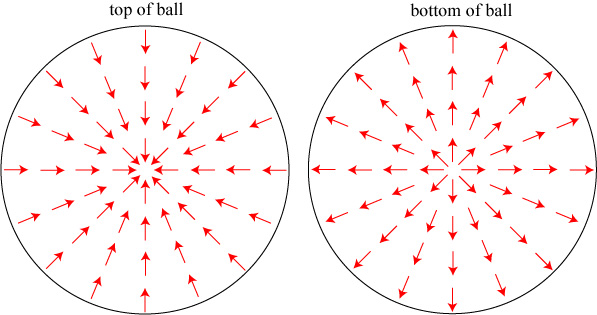
\includegraphics[scale=0.3]{Figs/inoutcomb.jpg}
    % \caption{Caption}
    % \label{fig:my_label}
\end{figure}
Hence, we can multiply any smooth vector field $v\in\Gamma(TS^2)$ by a function $f\in \mathcal{C}^\infty(S^2)$ which is zero everywhere except where $v$ is, obtaining $fv=0$ despite $f\neq 0$ and $v\neq 0$. Therefore, \tb{there is no set of linearly independent vector fields on $S^2$}, much less a basis.

\item \magenta{Locally, for vector, covector and general tensor fields on a manifold, we always have a basis using local chart.} See above \tb{(co-)vector fields locally from chart} and \tb{local representation of $n$-form} in next \cref{sec:grass}. This is because locally it behaves like $\Real^d$ as the above Example I.
\item \tb{\cyan{frame} of tangent bundle:}  We now give an example of the bases, called \tb{frame}, for  $\mathcal{C}^\infty(M)$-module property for $\Gamma(TM)$. An ordered $k$ tuple $\left(X_1, \ldots, X_k\right)$ of vector fields defined on some subset $A \subseteq M$
\begin{itemize}[$\ast$]
    \item is \tb{linearly independent} if $\left(\left.X_1\right|_p, \ldots,\left.X_k\right|_p\right)$ is a \tb{linearly independent} $k$-tuple in $T_p M$ for each $p \in A$, 
    \item \tb{spans the tangent bundle} if the $k$-tuple $\left(\left.X_1\right|_p, \ldots,\left.X_k\right|_p\right)$ spans $T_p M$ at each $p \in A$.
\end{itemize}
\begin{enumerate}
    \item\tb{local frame:} A \tb{local frame} for $M$ is an ordered $n$-tuple of vector fields $\left(E_1, \ldots, E_n\right)$ defined on an open subset $U \subseteq M$ that is \tb{linearly independent and spans the tangent bundle}. Thus the vectors $\left(\left.E_1\right|_p, \ldots,\left.E_n\right|_p\right)$ form a basis for $T_p M$ at each $p \in U$. 
    \item \tb{global frame and parallelizable:} It is called a \tb{global frame} if $U=M$. Global frames do not generally exist. If a manifold admits a \tb{global frame}, we call it  \tb{parallelizable}. 
\end{enumerate}
\begin{itemize}[$\circ$]
    \item \tb{notation:} We often use the shorthand notation $\left(E_i\right)$ to denote a frame $\left(E_1, \ldots, E_n\right)$. {\tiny So if $M$ has dimension $d$, then to check that an ordered $n$-tuple of vector fields $\left(E_1, \ldots, E_n\right)$ is a local frame, it suffices to check either that it is linearly independent or that it spans the tangent bundle. }
\item \tb{coordinate frame:} Recall the \tb{vector fields locally from chart} $U$ defined in the beginning of this section.  
\begin{align*} 
        \bigg\{ \bigg(\frac{\p}{\p x^1}\bigg), ... , \bigg(\frac{\p}{\p x^d}\bigg)\bigg\}
    \end{align*} 
    constitutes a basis for the tangent space $T_pM$ at each point $p$, and it's known as the \tb{coordinate frame basis}.
\item \tb{equivalent condition of parallelizable:}  ``tangent bundle over a manifold is trivial'' $\Leftrightarrow$ ``the manifold is paralelizable''. {\tiny Because if it's parallelizable, you can find a global frame field of the manifold. This frame field induces a bundle isomorphism to $M \times \mathbb{R}^n$. Conversely, if the tangent bundle is trivial, then a trivialization is a global frame field.}
\end{itemize}

\end{itemize}





\item \tb{direct sum of module:} 
The \tb{direct sum} of two $R$-modules $M$ and $N$ is the $R$-module $M\oplus N$, which has $M\times N$ as its underlying set and operations (inherited from $M$ and $N$) defined componentwise. 
\begin{itemize}
    \item \tb{notation:} While we have been using $\oplus$ to temporarily distinguish two ``plus-like'' operations in different spaces, the symbol $\oplus$ is the standard notation for the direct sum.
\end{itemize}
\item \tb{module terminology:}
An $R$-module $M$ is said to be
\begin{itemize}
\item \tb{finitely generated} if it has a finite generating set;
\item \tb{free} is it has a basis;
\item \tb{projective} if it is a direct \tb{summand} of a free $R$-module $F$, i.e.\
\bse
M \oplus Q = F
\ese
for some $R$-module $Q$.
\item 
If a \tb{finitely generated} module $R$-module $F$ is \tb{free}, and $d\in \N$ is the cardinality of a finite basis, then
\bse
F\cong_\mathrm{mod} = \underbrace{R\oplus\cdots\oplus R}_{d \text{ copies}} =: R^d.
\ese
One can show that if $R^d\cong_\mathrm{mod} R^{d'}$, then $d=d'$ and hence, \cyan{the concept of dimension is well-defined for finitely generated, free modules.}
\item Examples: 
\begin{itemize}[$\dagger$]
    \item $R\coloneqq\mathbb{Z} / 6 \mathbb{Z}$ a \tb{free} module over itself. Because $\mathbb{Z} / 2 \mathbb{Z} \oplus \mathbb{Z} / 3 \mathbb{Z} \cong R$, we have that $\mathbb{Z} / 2 \mathbb{Z}$, considered as an $R$-module, is \tb{projective}, but it is \tb{not free} since any non-trivial direct sum of $R$ (must take $R$ as a direct sum summand, otherwise the coefficient is not unique)  would have at least 6 elements.
    \item The Baer-Specker group $\bbZ^{\bbN}$, which is \tb{not finitely generated}, is an example of a \tb{torsion-free} $\mathbb{Z}$-module which is \tb{not free}.
    \item  $\Gamma(T\R^2)$ is free while $\Gamma(TS^2)$ is not. 
    \item Every free module is also projective.
\end{itemize}
\end{itemize}
\item \tb{$R$-linear map}
Let $M$ and $N$ be two (left) $R$-modules. A map $f\cl M \to N$ is said to be an \tb{$R$-linear map}, or an \tb{$R$-module homomorphism}, if
\bse
\forall \, r\in R : \forall \, m_1,m_2\in M : \ f(rm_1 + m_2)=rf(m_1)+f(m_2),
\ese
where it should be clear which operations are in $M$ and which in $N$.

\begin{itemize}
    \item \tb{module isomorphism}: A \tb{bijective module homomorphism}\footnote{Recall that the inverse of a bijective linear map is automatically linear.} is said to be a \tb{module isomorphism}, and we write $M\cong_{\mathrm{mod}}N$ if there exists a module isomorphism between them.
    \item \tb{right $R$-modules homomorphism:} If $M$ and $N$ are right $R$-modules, then the linearity condition is written as
\bse
\forall \, r\in R : \forall \, m_1,m_2\in M : \ f(m_1r + m_2)=f(m_1)r+f(m_2).
\ese
\end{itemize}

\item \tb{vector fibre bundle:} 
A \tb{vector fibre bundle} is a fibre bundle in which the fibre is a \tb{vector space}. 
\begin{itemize}
    \item Example:  tangent bundle to a manifold.
    \item \tb{Serre-Swan Theorem:} Let $E$ be a vector fibre bundle over a smooth manifold $M$. Then, the set $\Gamma(E)$ of all smooth section of $E$ over $M$ is a \tb{finitely generated, projective} $\mathcal{C}^\infty(M)$-module.
    \begin{itemize}[$\ast$]
        \item An immediate consequence of the theorem is that, for any vector fibre bundle $E$ over $M$, there exists a $\mathcal{C}^\infty(M)$-module $Q$ such that the direct sum $\Gamma(E)\oplus Q$ is free. If $Q$ can be chosen to be the trivial module $\{0\}$, then $\Gamma(E)$ is itself free, as it is the case with $\Gamma(T\R^2)$. In a sense, the module $Q$ \tb{quantifies the failure} of $\Gamma(E)$ to have a basis.
    \end{itemize}
\end{itemize}

\item \tb{hom-set:} Let $P,Q$ be finitely generated (projective) modules over a commutative ring $R$. Then
\bse
\Hom_R(P,Q) := \{\phi\cl P \xrightarrow{\sim} Q \mid \phi \text{ \normalfont is $R$-linear}\}
\ese
is again \tb{a finitely generated (projective) $R$-module}, with operations defined \cyan{pointwisely}.


\begin{itemize}
    \item \purple{\tb{covector field equivalent definition II:}} We have the \tb{dual of a module = covector field}, where the dual of a module is defined as
\bse
\Hom_{\mathcal{C}^\infty(M)}(\Gamma(TM),\mathcal{C}^\infty(M)) =: \Gamma(TM)^*.
\ese
One can show that $\Gamma(TM)^*$ coincides with $\Gamma(T^*M)$, i.e.\ the set of covector fields.
\end{itemize}


\item \tb{tensor field equivalent definition II:}
Let $M$ be a smooth manifold. A smooth \tb{$(r,s)$ tensor field} $\tau$ on $M$ is a \tb{$\mathcal{C}^\infty(M)$-multilinear map}
\bse
\tau\cl \underbrace{\Gamma(T^*M)\times \cdots \times \Gamma(T^*M)}_{r \text{ copies}} \times \underbrace{\Gamma(TM)\times \cdots \times \Gamma(TM)}_{s \text{ copies}} \to \mathcal{C}^\infty(M).
\ese

\begin{itemize}
    \item The equivalence of this to the bundle definition is due to the \cyan{\tb{pointwise nature of tensors}}. For instance, a covector field $\omega\in \Gamma(T^*M)$ can act on a vector field $X\in\Gamma(TM)$ to yield a smooth function $\omega(X)\in\mathcal{C}^\infty(M)$ by
\bse
(\omega(X))(p) := \omega(p)(X(p)).
\ese
Then, we see that for any $f\in\mathcal{C}^\infty(M)$, we have
\bse
(\omega(fX))(p) = \omega(p)(f(p)X(p)) = f(p)\omega(p)(X(p)) =: (f\omega(X))(p)
\ese
and hence, the map $\omega\cl \Gamma(TM)\xrightarrow{\sim}\mathcal{C}^\infty(M)$ is $\mathcal{C}^\infty(M)$-linear.
{\tiny \begin{itemize}[$\ast$]
    \item $fw(X)$ is inside the module $\Gamma(T^*M)$ is because of the above module property. Here it shows the $\mathcal{C}^{\infty}$-linear of the input variable  $X\in \Gamma(TM)$. So we have $\Gamma(T^*M)\subseteq$ ``the set of all the $\mathcal{C}^{\infty}$ maps from $\Gamma(TM)\rightarrow\mathcal{C}^{\infty}(M)$''. 
\item   But note, one $\mathcal{C}^{\infty}$-linear map $\Gamma(TM)\rightarrow\mathcal{C}^{\infty}(M)$ is mentioned in ``dual of a module''. So it is in $\Gamma(TM)^*$ (which can be shown then to be $\Gamma(T^*M)$)
\end{itemize}}
\item Similarly, the set $\Gamma(T^r_sM)$ of all $(r,s)$ smooth tensor fields on $M$ can be made into a $\mathcal{C}^\infty(M)$-module, with module operations defined \tb{pointwise}.
\item Therefore, we can think of tensor fields on $M$ either as sections of some tensor bundle on $M$ or as a $\mathcal{C}^\infty(M)$-multilinear map as above. 
\end{itemize}

\item \tb{tensor product:} We define the tensor product of tensor fields as:
\bi{rrCl}
\otimes \cl & \Gamma(T^p_qM) \times \Gamma(T^r_sM) & \to & \Gamma(T^{p+r}_{q+s}M)\\
&(\tau,\sigma) & \mapsto & \tau \otimes \sigma
\ei
analogously to what we had with tensors on a vector space, i.e.\
\bi{rl}
(\tau\otimes \sigma)(\omega_1,\ldots,\omega_p,\omega_{p+1},\ldots,\omega_{p+r},X_1,&\ldots,X_q,X_{q+1},\ldots,X_{q+s})\\
:=\tau(\omega_1,\ldots,\omega_p,X_1,&\ldots,X_q)\,\sigma(\omega_{p+1},\ldots,\omega_{p+r},X_{q+1},\ldots,X_{q+s}),
\ei
with $\omega_i\in \Gamma(T^*M)$ and $X_i\in \Gamma(TM)$.







\end{enumerate}

\section{Grassmann Algebra and De Rham Cohomology}\label{sec:grass}
In \cref{sec:tensorI}, we define \tb{$n$-form} (a special $(0, n)$-tensor) and volume (top) form. Using the field concepts from last \cref{sec:tensorII}, we now state the \tb{differential $n$-form}, which is a  \tb{$(0, n)$-tensor field}. All the concepts like Grassmann algebra, exterior derivative and de Rham cohomology are based on the differential forms.

A summary:
\begin{itemize}[$\blacktriangleright$]
\item We define \tb{differential $n$-form}, and recall the pull-back again, which is always well-defined according to previous sections.
\item We define the \tb{Grassmann algebra} for a manifold with the algebra dot product being the \tb{wedge (or called exterior) product}.
\item The \tb{exterior derivative} is then defined, and some properties are shown.
\item We finally define \tb{de Rham cohomology} using the concepts \tb{closed} and \tb{exact} from exterior derivative.
\end{itemize}
\begin{enumerate}
    \item Let $M$ be a smooth manifold. A \tb{differential $n$-form} on $M$ is a $(0,n)$ smooth \tb{tensor field} $\omega$ which is \tb{totally antisymmetric}, i.e.\
\bse
\omega(X_1,\ldots,X_n) = \sgn(\pi)\, \omega(X_{\pi(1)},\ldots,X_{\pi(n)}),
\ese
for any $\pi \in S_n$, with $X_i\in \Gamma(TM)$.  
    \begin{itemize}
        \item Sometimes, we simply called \tb{differential $n$-form} as \tb{$n$-form}. But please don't mix up with the \cyan{tensor} $n$-form. Here \tb{$n$-form} indicates a \cyan{tensor field}.
        \item \tb{orientable:} A manifold $M$ is said to be \tb{orientable} if it admits an oriented atlas, i.e.\ an atlas in which all chart transition maps, which are maps between open subsets of $\R^{\dim M}$, have a \tb{positive determinant}.
        \begin{itemize}[$\ast$]
            \item If $M$ is orientable, then there exists a nowhere vanishing top form ($n=\dim M$) on $M$ providing the volume.
        \end{itemize}
        \item \tb{degree:} If $\omega$ is an $n$-form, then $n$ is said to be the \tb{degree} of $\omega$.
        \item  \tb{notation:} We denote by $\Omega^n(M)$ the set of all differential $n$-forms on $M$, which then becomes a $\mathcal{C}^\infty(M)$-module by defining the addition and multiplication operations \cyan{pointwise on $M$}.
        \begin{itemize}[$\ast$]
            \item So we have $\Omega^0(M)\equiv \mathcal{C}^\infty(M)$ and $\Omega^1(M)\equiv \Gamma(T^0_1M)\equiv\Gamma(T^*M)$.
        \end{itemize}
        \item Similar to the \tb{tensor $n$-form}, we have $\Omega^n(M)=\{0\}$ for $n>\dim M$.%, and otherwise $\dim \Omega^n(M)= {{\dim M}\choose{n}}$, as a $\mathcal{C}^\infty(M)$-module.
    \end{itemize}
    
\item \tb{(global) pull-back of differential forms:} Note, we have defined the general pull-back of \tb{contravariant field} in the last \cref{sec:tensorII} which is always well-defined. Here we just specialise the pull-back to differential forms since {differential $n$-form is special \tb{contravariant $n$-tensor field}.} 
Let $\phi\cl M \to N$ be a smooth map and let $\omega\in \Omega^n(N)$. Then we define the \tb{pull-back} $\Phi^*(\omega)\in \Omega^n(M)$ of $\omega$ as
\bi{rrCl}
\Phi^*(\omega)\cl & M &\to & T^*M\\
& p & \mapsto & \Phi^*(\omega) (p), 
\ei
where
\bse
\Phi^*(\omega)(p)(X_1,\ldots,X_n):=\omega (\phi(p))\bigl( \phi_*(X_1),\ldots,\phi_*(X_n) \bigr),
\ese
for $X_i\in T_pM$.
\begin{itemize}
    \item The map $\Phi^*$ on $\Omega^0(M)$ is simply
\bi{rrCl}
\Phi^*\cl & \Omega^0(M) & \to & \Omega^0(M)\\
&f &\mapsto &\Phi^*(f) := f\circ \phi.
\ei
\end{itemize}

\item \tb{wedge (exterior) product}
Let $M$ be a smooth manifold. We define the \tb{wedge (exterior) product} of forms as the map
\bi{rrCl}
\wedge \cl & \Omega^n(M) \times \Omega^m(M) & \to & \Omega^{n+m}(M)\\
& (\omega,\sigma) & \mapsto & \omega \wedge \sigma,
\ei
where
\bse
(\omega\wedge\sigma)(X_1,\ldots,X_{n+m}) := \frac{1}{n!\,m!} \sum_{\pi \in S_{n+m}} \sgn(\pi) (\omega \otimes \sigma)(X_{\pi(1)},\ldots,X_{\pi(n+m)})
\ese
and $X_1,\ldots,X_{n+m}\in\Gamma(TM)$. 
\begin{itemize}
    \item \tb{notation:} By convention, for any $f,g\in \Omega^0(M)$ and $\omega\in \Omega^n(M)$, we set
\bse
f\wedge g := fg \qquad \text{and} \qquad f\wedge\omega=\omega\wedge f = f\omega.
\ese
\item \tb{Why not just using the tensor product?} Because the tensor product of two forms is not necessarily still a form, i.e. \tb{satisfying totally antisymmetric}. 

\item \tb{The wedge product is  $\mathcal{C}^\infty(M)$-bilinear:} \bse
(f\omega_1 +\omega_2)\wedge \sigma = f\, \omega_1\wedge\sigma+\omega_2\wedge\sigma,
\ese
for all $f\in\mathcal{C}^\infty(M)$, $\omega_1,\omega_2\in\Omega^n(M)$ and $\sigma\in\Omega^m(M)$, and similarly for the second argument. 
\begin{itemize}[$\ast$]
    \item This will be used later to define the \tb{Grassmann algebra dot product.}
\end{itemize}

\item  \tb{graded commutative of $\wedge$ over \cyan{single $n$-form}:} Let $\omega\in\Omega^n(M)$ and $\sigma\in\Omega^m(M)$. Then
\bse
\omega\wedge\sigma=(-1)^{nm}\,\sigma\wedge\omega.
\ese
We say that $\wedge$ is \tb{graded commutative}, that is, it satisfies a version of anticommutativity which depends on the degrees of the forms.

\item Example: Suppose that $\omega,\sigma\in\Omega^1(M)$. Then, for any $X,Y\in\Gamma(TM)$
\bi{rCl}
(\omega\wedge\sigma)(X,Y) & = & (\omega\otimes\sigma)(X,Y) - (\omega\otimes\sigma)(Y,X)\\
& = & (\omega\otimes\sigma)(X,Y) - \omega(Y)\sigma(X)\\
& = & (\omega\otimes\sigma)(X,Y) - (\sigma \otimes \omega)(X,Y)\\
& = & (\omega\otimes\sigma -\sigma \otimes \omega)(X,Y).
\ei
Hence
\bse
\omega\wedge\sigma = \omega\otimes\sigma - \sigma \otimes \omega. 
\ese
Note is only true when $\omega$ and $\sigma$ are \cyan{pure degree forms}, rather than linear combinations of forms of different degrees.
\end{itemize}

\item \tb{\purple{local representation} of $n$-form:}
If $(U,x)$ is a chart on $M$, then every $n$-form $\omega\in \Omega^n(U)$ can be expressed \tb{locally} on $U$ as
\bse
\omega = \omega_{a_1\cdots a_n} \, \d x^{a_1} \wedge \cdots \wedge \d x^{a_n},
\ese
where $\omega_{a_1\cdots a_n}\in \mathcal{C}^\infty(U)$, $1\leq a_1 < \cdots < a_n \leq \dim M$ are increasing sequence and $\d x^{a_1} \wedge \cdots \wedge \d x^{a_n}$ has been defined as above.
\begin{itemize}
    \item The $\d x^{a_i}$ appearing above are the covector fields ($1$-forms) appeared in last \cref{sec:tensorII}:
\bse
\d x^{a_i} \cl p\mapsto \d_px^{a_i}.
\ese
% \item \tb{notation: }

\item \tb{wedge product in \purple{local representation}:} If  $\omega=\omega_{a_1\cdots a_n} \, \d x^{a_1} \wedge \cdots \wedge \d x^{a_n}$, and $\lambda=\lambda_{b_1\cdots a_m} \, \d x^{b_1} \wedge \cdots \wedge \d x^{b_m}$, we have
$$\omega \wedge \lambda=\omega_{a_1\cdots a_n} \lambda_{b_1\cdots a_m} (\d x^{a_1} \wedge \cdots \wedge \d x^{a_n})\wedge (\d x^{b_1} \wedge \cdots \wedge \d x^{b_m}).$$
\item \tb{pull-back in  \purple{local representation}:} {\tiny Assume that $x^1, \ldots, x^{\dim M}$ are coordinates on $M$, that $y^1$, $\ldots, y^{\dim N}$ are coordinates on $N$, and that these coordinate systems are related by the formulas $y^i=\phi_i\left(x^1, \ldots, x^{\dim M}\right)$ for all $i$. Locally on $N, \omega$ can be written as
\begin{align*}
\omega=\omega_{i_1 \cdots i_k} \d y^{i_1} \wedge \cdots \wedge \d y^{i_k},
\end{align*}
where, $i_1<\cdots<i_k$ and  for each choice of $i_1, \ldots, i_k, \omega_{i_1 \cdots i_k}$ is a real-valued function of $y^1, \ldots, y^{\dim N}$.} Using the \tb{linearity} of pullback and its \tb{compatibility with exterior product} (See \tb{a summary of pull-back}), the pullback of $\omega$ has the formula
\begin{align*}
\Phi^* \omega=\sum_{i_1<\cdots<i_k}\left(\omega_{i_1 \cdots i_k} \circ \phi\right) \d \phi_{i_1} \wedge \cdots \wedge \d \phi_{i_k} .
\end{align*}
Each exterior derivative $\d \phi_i$ can be expanded in terms of $\d x^1, \ldots, \d x^{\dim M}$. The resulting $k$-form can be written using \tb{Jacobian matrices}:
\begin{align*}
\Phi^* \omega=\sum_{i_1<\cdots<i_k} \sum_{j_1<\cdots<j_k}\left(\omega_{i_1 \cdots i_k} \circ \phi\right) \frac{\partial\left(\phi_{i_1}, \ldots, \phi_{i_k}\right)}{\partial\left(x^{j_1}, \ldots, x^{j_k}\right)} \d x^{j_1} \wedge \cdots \wedge \d x^{j_k} .
\end{align*}
Here, $\frac{\partial\left(\phi_{i_1}, \ldots, \phi_{i_k}\right)}{\partial\left(x^{j_1}, \ldots, x^{j_k}\right)}$ denotes the \tb{determinant} of the Jacobian matrix.
\magenta{So rudin \cite{rudin1976principles}[Definition 10.11] can be viewed from the manifold perspective! In rudin, we take map from $\R^m$ to a surface in $\R^n$ with $m\le n$.}
\item Compare with ruding: 
\begin{itemize}[$\ast$]
    \item In rudin, we directly define forms using local representation. The real meaning of the forms are reflected in integration \cite{rudin1976principles}[section 10, eq. 35]. The \tb{totally antisymmetric} comes from the \tb{determinant} of the Jacobian matrix.
    \item In this course, the differential form are defined using tensor fields with  \tb{totally antisymmetric} requirement. The integrand after pull-back will then have the  \tb{determinant}.
\end{itemize}
So \cyan{\tb{Jacobian determinant =  \tb{totally antisymmetric}} }
\end{itemize}
    
    
\item \tb{Grassmann algebra:} We first introduce a space which is closed under the action of  wedge product $\wedge$:
Let $M$ be a smooth manifold. Define the $\mathcal{C}^\infty(M)$-module
\bse
\Gr(M)\equiv\Omega(M) := \bigoplus_{n=0}^{\dim M} \Omega^n(M).
\ese
The \tb{Grassmann algebra} on $M$ is the algebra $(\Omega(M),+,\cdot,\wedge)$, where
\bse
\wedge\cl \Omega(M)\times\Omega(M)\to\Omega(M)
\ese
is the extension of the previously defined $\wedge\cl\Omega^n(M)\times\Omega^m(M)\to\Omega^{n+m}(M)$.


\begin{itemize}
    \item Direct sum of modules has the Cartesian product of the modules as underlying set and module operations defined \tb{componentwise}.
    \item ``Algebra'' here we really mean \tb{``algebra over a module''}.
    \item Example: Let $\psi=\omega+\sigma$, where $\omega\in\Omega^1(M)$ and $\sigma\in\Omega^3(M)$. Of course, this ``+'' is neither the addition on $\Omega^1(M)$ nor the one on $\Omega^3(M)$, but rather that on $\Omega(M)$.
\end{itemize}

\item \tb{commutator (Lie bracket):} Let $M$ be a smooth manifold and let $X,Y\in\Gamma(TM)$. The \tb{commutator (or Lie bracket)} of $X$ and $Y$ is defined as
\bi{rrCl}
[X,Y]\cl & \mathcal{C}^\infty(M) &\xrightarrow{\sim} &\mathcal{C}^\infty(M)\\ 
& f & \mapsto & [X,Y](f):=X(Y(f))-Y(X(f)),
\ei
where we are using the definition of vector fields as $\R$-linear maps $\mathcal{C}^\infty(M) \xrightarrow{\sim} \mathcal{C}^\infty(M)$.
\begin{itemize}
    \item This commutator is used to defined the \tb{exterior derivative} below.
    \item \tb{Lie algebra from commutator:} We use this commutator to define a \tb{Lie algebra} $(\Gamma(T M),+, \cdot,[-,-])$ over $\R$. According to the definition of \tb{Lie algebra} in 
    \cref{sec:tangent}, we need to check $\Real$-bilinear (as a algebra product), alternativity and the Jacobi identity (additional condition of the $[-,-]$ operator).
    \item The brackets appear everywhere when you want to obtain natura tensors on your manifold. Maybe the simplest example of this is the torsion operator of a connection. $T(X, Y)=\nabla_X Y-\nabla_Y X$ is \tb{not tensorial} in $X$ and $Y$. Indeed, $T(f X, Y)=f\left(\nabla_X Y-\nabla_Y X\right)-(Y . f) X$. The last term involves the derivative of $f$ and you want to get rid of it. Now observe that \cyan{$$[f X, Y]=f[X, Y]-(Y(f))\cdot X$$} so the same term appears in the non-tensoriality of the bracket. This leads to the good definition of the torsion: $T(X, Y)=\nabla_X Y-\nabla_Y X-[X, Y]$ and this is \tb{tensorial} in $X$ and $Y$.
\item Due to Schwarz's theorem on symmetric second derivatives, we have \green{$$\left[\frac{\p}{\p x^i},\frac{\p}{\p x^j}\right]=0.$$} This is very useful and can be used to get \tb{local representations}.
\end{itemize}

\item \tb{exterior derivative:}  
The \tb{exterior derivative} on $M$ is the $\R$-linear operator
\bi{rrCl}
\d\cl &\Omega^n(M)&\xrightarrow{\sim} &\Omega^{n+1}(M)\\
& \omega & \mapsto & \d \omega
\ei
with $\d \omega$ being defined as
\bi{rCl}
\d \omega (X_1,\ldots,X_{n+1}) & := & \sum_{i=1}^{n+1} (-1)^{i+1}\, X_i \bigl(\omega(X_1,\ldots,\widehat{X_i},\ldots,X_{n+1})\bigr)\\
& & {} \negmedspace + \sum_{i<j} (-1)^{i+j}\,\omega\bigl([X_i,X_j],X_1,\ldots,\widehat{X_i},\ldots,\widehat{X_j},\ldots,X_{n+1}\bigr),
\ei
where $X_i\in \Gamma(TM)$ and the hat denotes omissions.

\begin{itemize}
\item This map is antisymmetric: this follows quite immediately from the fact that $\omega$ itself is antisymmetric and that the bracket is ; 2) that this map is tensorial: this is really the crucial point. As we have mentioned above, Lie brackets appear here to ensure tensorial.
{\tiny  Denote the right hand side as $\widetilde{d \omega}$. We have \begin{align*}
\begin{aligned}
\widetilde{d \omega}\left(f X_1, X_2, \cdots, X_{k+1}\right)=& f X_1\left(\omega\left(X_2, \cdots, X_{k+1}\right)\right) \\
&+\sum_{i>1}(-1)^{i-1} X_i\left(\omega\left(f X_1, \cdots, \widehat{X_i}, \cdots, X_{k+1}\right)\right) \\
&+\sum_{i>1}(-1)^{i+1} \omega\left(\left[f X_1, X_i\right], X_2, \cdots, \widehat{X_i}, \cdots, X_{k+1}\right) \\
&+\sum_{1<i<j}(-1)^{i+j} \omega\left(\left[X_i, X_j\right], f X_1, \cdots, \widehat{X_i}, \cdots, \widehat{X_j}, \cdots, X_{k+1}\right) \\
=& f \widetilde{d \omega}\left(X_1, \cdots, X_{k+1}\right) \\
&+\sum_{i>1}(-1)^{i-1}\left(X_i f\right) \omega\left(X_1, \cdots, \widehat{X}_i, \cdots, X_{k+1}\right) \\
&-\sum_{i>1}(-1)^{i+1}\left(X_i f\right) \omega\left(X_1, \cdots, \widehat{X}_i, \cdots, X_{k+1}\right) \\
=& f \widetilde{d \omega}\left(X_1, \cdots, X_{k+1}\right) .
\end{aligned}
\end{align*}
}
\item Don't be confused, $\R$-linear is \gls{wrt} $\d(\text{input})$, while the $\calC^\infty$-linear is \gls{wrt} $\d \omega (\text{input})$. $\d(\text{input})$ is not $\calC^\infty$-linear, instead it satisfies the following \tb{Leibniz rule}.
    \item \tb{compare to covariant derivative:} That the operator $\d$ is only well-defined when it acts on forms, i.e., \tb{contravariant tensor field}. In order to define a derivative operator on \tb{covariant and general tensor fields} we will need to add extra structure, called \tb{connection}, to our differentiable manifold.
    \item \tb{relation to differential operator $\d_p$ in \cref{sec:cotangent}:} We can extend that definition in \cref{sec:cotangent} to define the following ($\R$-linear) operator:
\bi{rrCl}
\d \cl & \mathcal{C}^\infty(M) & \xrightarrow{\sim} & \Gamma(T^*M)\\
& f & \mapsto & \d f
\ei
where, of course, $\d f \cl p \mapsto \d_pf$. 
\begin{itemize}[$\ast$]
\item So, we can also understand this as an example of \tb{exterior derivative} that takes in $0$-forms and outputs $1$-forms
\bse
\d \cl \Omega^0(M)\xrightarrow{\sim}\Omega^1(M).
\ese {\tiny Alternatively, we can view  $\d f$ as the \tb{$\R$-linear map}
\bi{rrCl}
\d f \cl & \Gamma(TM) & \xrightarrow{\sim} & \mathcal{C}^\infty(M)\\
& X &\mapsto & \d f (X) = X(f).
\ei}
    \item \tb{\purple{local representation}:} {\tiny As we mentioned above, locally on some chart $(U,x)$ on $M$, the covector field (or $1$-form) $\d f$ can be expressed as
\bse
\d f = \lambda_a\, \d x^a
\ese
for some smooth functions $\lambda_i\in\mathcal{C}^\infty(U)$. To determine what they are, we simply apply \emph{both sides} to the vector fields induced by the chart. We have
\bse
\d f \biggl( \frac{\partial}{\partial x^b}\biggr) =  \frac{\partial}{\partial x^b}(f) = \partial_bf
\ese
and
\bse
\lambda_a\, \d x^a\biggl( \frac{\partial}{\partial x^b}\biggr) =\lambda_a\,  \frac{\partial}{\partial x^b}(x^a) = \lambda_a\,\delta^a_b = \lambda_b.
\ese}
Hence, the local expression of $\d f$ on $(U,x)$ is
\purple{\bse
\d f = \partial_a f \, \d x^a.
\ese}
\item \tb{Leibniz rule:} Note that the operator $\d$ satisfies the Leibniz rule
\bse
\d (fg) = g\, \d f + f\, \d g.
\ese
\end{itemize}
\item \tb{general \purple{local representation}:} {\tiny From linearity, so without loss of generality, we may first assume
\begin{align*}
\omega=f \d x^1 \wedge \cdots \wedge \d x^k
\end{align*}
in a local chart $U$. Note that \green{$\left[\partial_i, \partial_j\right]=0$.} It follows that for any increasing indices $j_1<\cdots<j_{k+1}$, the right hand side of
\begin{align*}
\widetilde{\d \omega}\left(\partial_{j_1}, \cdots, \partial_{j_{k+1}}\right)=\sum_i(-1)^{i-1} \partial_{j_i}\left(\omega\left(\partial_{j_1}, \cdots, \hat{\partial}_{j_i}, \cdots, \partial_{j_{k+1}}\right)\right)
\end{align*}
vanishes except for the case $j_1=1, \cdots, j_k=k$ and $i=k+1$ (and thus $\left.j_i \geq k+1\right)$. In other words, the only non-zero terms in all possible expressions $\widetilde{\d \omega}\left(\partial_{j_1}, \cdots, \partial_{j_{k+1}}\right)$ are
\begin{align*}
\widetilde{\d \omega}\left(\partial_1, \cdots, \partial_k, \partial_r\right)=(-1)^k \partial_r(f) .
\end{align*}
It follows that
\begin{align*}
\widetilde{\d \omega}=\sum_{r>k}(-1)^k \partial_r(f) \d x^1 \wedge \cdots \wedge \d x^k \wedge \d x^r=\sum \partial_r(f) \d x^r \wedge \d x^1 \wedge \cdots \wedge \d x^k.
\end{align*} 
From linearity,}
\purple{now suppose $\omega$ is a $k$-form on $M$, so that locally
\bse
\omega = \omega_{a_1\cdots a_n}\d x^{a_1}\wedge \cdots \wedge \d x^{a_n}.
\ese
Then, we have
\bi{rCl}
\d \omega & = & \d \omega_{a_1\cdots a_n}\wedge\d x^{a_1}\wedge \cdots \wedge \d x^{a_n}\\
 & = & \partial_b \omega_{a_1\cdots a_n}\d x^b\wedge\d x^{a_1}\wedge \cdots \wedge \d x^{a_n},
\ei}

% \item Example: {\tiny In the case $n=1$, the form $\d \omega\in\Omega^2(M)$ is given by
% \bse
% \d \omega (X,Y) = X(\omega(Y))-Y(\omega(X))-\omega([X,Y]).
% \ese
% Let us check that this is indeed a $2$-form, i.e.\ an antisymmetric, $\mathcal{C}^\infty(M)$-multilinear map
% \bse
% \d\omega\cl \Gamma(TM)\times\Gamma(TM)\to\mathcal{C}^\infty(M).
% \ese
% By using the antisymmetry of the Lie bracket, we immediately get
% \bse
% \d \omega(X,Y)= - \,\d\omega(Y,X).
% \ese
% Moreover, thanks to this identity, it suffices to check $\mathcal{C}^\infty(M)$-linearity in the first argument only. Additivity is easily checked
% \bi{rCl}
% \d\omega(X_1+X_2,Y) & = & (X_1+X_2)(\omega(Y))-Y(\omega(X_1+X_2))-\omega([X_1+X_2,Y])\\
% & = & X_1(\omega(Y))+X_2(\omega(Y))-Y(\omega(X_1)+\omega(X_2))-\omega([X_1,Y]+[X_2,Y])\\
% & = & X_1(\omega(Y))+X_2(\omega(Y))-Y(\omega(X_1))-Y(\omega(X_2))-\omega([X_1,Y])-\omega([X_2,Y])\\
% &=& \d\omega(X_1,Y) +\d\omega(X_2,Y).
% \ei
% For $\mathcal{C}^\infty(M)$-scaling, first we calculate $[fX,Y]$. Let $g\in\mathcal{C}^\infty(M)$. Then
% \bi{rCl}
% [fX,Y](g) &=& fX(Y(g)) -Y (fX(g))\\
% &=& fX(Y(g)) - fY(X(g)) -Y (f)X(g)\\
% &=& f(X(Y(g)) - Y(X(g))) -Y (f)X(g)\\
% &=& f[X,Y](g) -Y(f)X(g)\\
% &=& (f[X,Y] -Y(f)X)(g).
% \ei
% Therefore
% \bse
% [fX,Y]=f[X,Y]-Y(f)X.
% \ese
% Hence, we can calculate
% \bi{rCl}
% \d\omega(fX,Y) & = & fX(\omega(Y))-Y(\omega(fX))-\omega([fX,Y])\\
% & = & fX(\omega(Y))-Y(f\omega(X))-\omega(f[X,Y]-Y(f)X)\\
% & = & fX(\omega(Y))-fY(\omega(X))-Y(f)\omega(X)-f\omega([X,Y])+\omega(Y(f)X)\\
% & = & fX(\omega(Y))-fY(\omega(X))-\Ccancel[gray]{Y(f)\omega(X)}-f\omega([X,Y])+\Ccancel[gray]{Y(f)\omega(X)}\\
% &=& f\,\d\omega(X,Y), 
% \ei
% which is what we wanted.}
% \end{itemize}
\item \tb{graded Leibniz rule \gls{wrt} the wedge product:}
Let $\omega\in\Omega^n(M)$ and $\sigma\in\Omega^m(M)$. Then
\bse
\d(\omega\wedge\sigma)=\d\omega\wedge\sigma+(-1)^n\,\omega\wedge\d\sigma.
\ese

\end{itemize}
\item \tb{symplectic manifold:}
Let $M$ be a smooth manifold. A \tb{$2$-form} $\omega\in\Omega^2(M)$ is said to be a \tb{symplectic form} on $M$ if
\begin{enumerate}
    \item $\d \omega = 0$ and
    \item it is \tb{non-degenerate}, i.e.\
\bse
(\forall \, Y\in \Gamma(TM) : \omega(X,Y) = 0) \Rightarrow X = 0.
\ese
\end{enumerate} 
A manifold equipped with a symplectic form is called a \tb{symplectic manifold}.
\begin{itemize}
    \item \magenta{\tb{difference with Riemannian manifolds:} The metric tensor for Riemannian manifolds is \tb{symmetric}. So the key is nondegenerate bilinear forms that are \tb{symmetric vs. alternating.}} 
\end{itemize}
% In the Hamiltonian formulation of classical mechanics one is especially interested in the cotangent bundle $T^*Q$ of some configuration space $Q$. Similarly to what we did when we introduced the tangent bundle, we can define (at least locally) a system of coordinates on $T^*Q$ by
% \bse
% (q^1,\ldots,q^{\dim Q},p_1,\ldots,p_{\dim Q}),
% \ese
% where the $p_i$'s are the generalised momenta on $Q$ and the $q^i$'s are the generalised coordinates on $Q$ (recall that $\dim T^*Q=2\dim Q$). We can then define a $1$-form $\theta\in\Omega^1(T^*Q)$ by
% \bse
% \theta := p_i \, \d q^i
% \ese
% called the symplectic potential. If we further define
% \bse
% \omega := \d \theta \in \Omega^2(T^*Q),
% \ese
% then we can calculate that
% \bse
% \d \omega = \d (\d \theta) =\cdots = 0.
% \ese
% Moreover, $\omega$ is non-degenerate and hence it is a symplectic form on $T^*Q$.


\item \tb{a summary of pull-back of $n$-form:}
\begin{itemize}
    \item \tb{distribute over the wedge product:}

Let $\phi\cl M\to N$ be smooth, $\omega\in\Omega^n(N)$ and $\sigma\in\Omega^m(N)$. Then, we have
\bse
\Phi^*(\omega\wedge\sigma) = \Phi^*(\omega)\wedge\Phi^*(\sigma).  
\ese
\item  \tb{commute with wedge product:}
Let $\phi\cl M\to N$ be smooth. For any $\omega\in\Omega^n(N)$, we have
\bse
\Phi^*(\d \omega) = \d (\Phi^*(\omega)).
\ese
\item \tb{$\Real$-linear:}
\begin{align*}
    \Phi^*(c\sigma) &= c\Phi^*(\sigma),\\
\Phi^*(\omega+\sigma) &= \Phi^*(\omega)+\Phi^*(\sigma).  
\end{align*}
\end{itemize}

\item \tb{closed and exact:}
Let $M$ be a smooth manifold and let $\omega \in \Omega^n(M)$. We say that $\omega$ is
\begin{itemize}
\item \tb{closed} if $\d \omega = 0$;
\item \tb{exact} if $\exists \, \sigma \in \Omega^{n-1}(M): \omega = \d \sigma$.
\end{itemize}

\item \magenta{\tb{exact implies closed:}}
Let $M$ be a smooth manifold. The operator
\bse
\d^2 \equiv \d \circ \d \cl \Omega^n(M) \to \Omega^{n+2}(M)
\ese
is identically zero, i.e.\ $\d^2=0$.

\begin{itemize}
    \item \tb{{antisymmetrization and symmetrization}}: Given an object which carries some indices, say $T_{a_1,\ldots,a_n}$, we define the \tb{antisymmetrization} of $T_{a_1,\ldots,a_n}$ as
\bse
T_{[a_1\cdots a_n]}:=\frac{1}{n!}\sum_{\pi\in S_n}\sgn(\pi)\, T_{\pi(a_1)\cdots\pi(a_n)}.
\ese
Similarly, the \tb{symmetrization} of $T_{a_1,\ldots,a_n}$ is defined as
\bse
T_{(a_1\cdots a_n)}:=\frac{1}{n!}\sum_{\pi\in S_n} T_{\pi(a_1)\cdots\pi(a_n)}.
\ese
\begin{itemize}[$\ast$]
    \item Examples:{\tiny
\bi{C}
T_{[ab]}=\frac{1}{2}(T_{ab}-T_{ba}), \qquad 
T_{(ab)}=\frac{1}{2}(T_{ab}+T_{ba}) \\
T_{[abc]} = \frac{1}{6} (T_{abc}+T_{bca}+T_{cab}-T_{bac}-T_{cba}-T_{acb})\\
T_{(abc)} = \frac{1}{6} (T_{abc}+T_{bca}+T_{cab}+T_{bac}+T_{cba}+T_{acb})
\ei}
\item Of course, we can (anti)symmetrize only some of the indices
\bse
T^{ab}_{\phantom{ab}[cd]e} = \frac{1}{2}(T^{ab}_{\phantom{ab}cde}-T^{ab}_{\phantom{ab}dce}).
\ese
\item It is easy to check that in a \tb{contraction} (i.e.\ a sum), we have
\bse
T_{a_1\cdots a_n}S^{a_1\cdots [a_i \cdots a_j] \cdots a_n} = T_{a_1\cdots [a_i \cdots a_j] \cdots a_n}S^{a_1 \cdots a_n} 
\ese
and
\bse
T_{a_1\cdots (a_i \cdots a_j) \cdots a_n}S^{a_1\cdots [a_i \cdots a_j] \cdots a_n} = 0.
\ese
\end{itemize}
\item proof sketch: {\tiny
\bi{rCl}
\d^2\omega & = & \partial_c\partial_b\omega_{a_1\cdots a_n}\d x^c\wedge\d x^b\wedge\d x^{a_1}\wedge \cdots \wedge \d x^{a_n}\\
& = & \partial_{(c}\partial_{b)}\omega_{a_1\cdots a_n}\d x^{[c}\wedge\d x^{b]}\wedge\d x^{a_1}\wedge \cdots \wedge \d x^{a_n}\\
& = & 0.
\ei
Since this holds for any $\omega$, we have $\d^2=0$.}
\end{itemize}
\item \tb{de Rham cohomology:}
We can extend the action of $\d$ to the zero vector space $0:=\{0\}$ by mapping the zero in $0$ to the zero function in $\Omega^0(M)$. In this way, we obtain the chain of $\R$-linear maps
% \bse
% \begin{tikzcd}
% 0 \ar[r,"\d"]& \Omega^0(M)\ar[r,"\d"]&\cdots\ar[r,"\d"]& \Omega^n(M)\ar[r,"\d"]& \Omega^{n+1}(M)\ar[r,"\d"]& \cdots \ar[r,"\d"]& \Omega^{\dim M}(M)\ar[r,"\d"] & 0
% \end{tikzcd}
% \ese
\bse
0 \xrightarrow{\ \d\ } \Omega^0(M)\xrightarrow{\ \d\ } \Omega^1(M)\xrightarrow{\ \d\ } \cdots \xrightarrow{\ \d\ } \Omega^{n}(M)\xrightarrow{\ \d\ } \Omega^{n+1}(M)\xrightarrow{\ \d\ } \cdots \xrightarrow{\ \d\ } \Omega^{\dim M}(M)\xrightarrow{\ \d\ } 0,
\ese
where we now think of the spaces $\Omega^n(M)$ as $\R$-vector spaces. 
The equation $\d^2=0$ is equivalent to
\bse
\im(\d \cl \Omega^n(M)\to\Omega^{n+1}(M)) \se \ker(\d \cl \Omega^{n+1}(M)\to\Omega^{n+2}(M))
\ese
% \bse
% \im(\Omega^n(M)\xrightarrow{\ \d \ }\Omega^{n+1}(M)) \se \ker(\d \cl \Omega^{n+1}(M)\xrightarrow{\ \d \ }\Omega^{n+2}(M))
% \ese
for all $0\leq n \leq \dim M-2$. Moreover, we have
\bi{rCl}
\omega \in \Omega^n(M) \text{ is closed } & \Leftrightarrow\ & \omega \in \ker(\d \cl \Omega^n(M)\to\Omega^{n+1}(M))\\
\omega \in \Omega^n(M) \text{ is exact } & \Leftrightarrow\ & \omega \in \im (\d \cl \Omega^{n-1}(M)\to\Omega^{n}(M)).
\ei
\begin{itemize}
    \item \tb{notation:} \bi{rCl}
Z^n & := & \ker(\d \cl \Omega^n(M)\to\Omega^{n+1}(M)),\\
B^n & := & \im (\d \cl \Omega^{n-1}(M)\to\Omega^{n}(M)),
\ei
so that $Z^n$ is the space of closed $n$-forms and $B^n$ is the space of exact $n$-forms.
\begin{itemize}[$\ast$]
    \item $\d^2=0$ implies that $B^n\se Z^n$ for all $n$. \cyan{So $B^n$ is a vector subspace of $Z^n$.}
\end{itemize}
    \item \pink{\tb{question:}} We have the question of whether every closed form is exact and vice versa, i.e.\ whether the implications 
\bse
Z^n=B^n
\ese
hold in general.  The answer is \tb{no} in general.
\item \tb{special simply connected domain (Poincar\'e lemma):}  Let $M\se \R^d$ be a simply connected domain. Then
\bse
Z^n = B^n \, , \qquad \forall \, n > 0.
\ese
\item \tb{de Rham cohomology group:} %In the cases where $Z^n\neq B^n$, we would like to quantify by how much the closed $n$-forms fail to be exact. 
Let $M$ be a smooth manifold. The $n$-th \tb{de Rham cohomology group} on $M$ is the quotient $\R$-vector space
\bse
H^n(M):=Z^n/B^n.
\ese
\begin{itemize}[$\ast$]
    \item It is a quotient group as $Z^n/\!\sim$, where $\sim$ is the equivalence relation $\omega \sim \sigma\ :\Leftrightarrow\ \omega-\sigma \in B^n$.
    \item \pink{\tb{question reformulation:}} Does the following is true
\bse
H^n(M) \cong_\mathrm{vec} 0.
\ese
\item de Rham states that $H^n(M)$ only depends on the global topology of $M$. In other words, \magenta{the cohomology groups are topological invariants.} This is remarkable because $H^n(M)$ is defined in terms of exterior derivatives, which have everything to do with the local differentiable structure of $M$, and a given topological space can be equipped with several inequivalent differentiable structures. 
\item Example I: Let $M$ be any smooth manifold. We have
\bse
H^0(M) \cong_\mathrm{vec} \R^{\text{(\# of connected components of $M$)}}
\ese
since the closed $0$-forms are just the locally constant smooth functions on $M$. As an immediate consequence, we have
\bse
H^0(\R) \cong_\mathrm{vec} H^0(S^1) \cong_\mathrm{vec} \R.
\ese
\item Example II:
By Poincar\'e lemma, we have
\bse
H^n(M) \cong_\mathrm{vec} 0
\ese
for any simply connected $M\se\R^d$. In \cite{rudin1976principles}[Theorem 10.39,] the convex and open set is a speical case of the simply connected.
\end{itemize}




\end{itemize}




    
    
\end{enumerate}


\section{Lie Groups and Their Associated Lie Algebras}\label{sec:lie}

\adjustbox{center}{
\tikzset{LA/.style = {draw=red, % just to demonstrate, where LA is used
                      line width=#1,-{Straight Barb[length=3pt]}},
         LA/.default=1pt
        }
\begin{tikzcd}[row sep=0.5cm,column sep=0.5cm, color=black]
% b  & D\arrow[d,"\text{text}"] & b \\
\text{set} \arrow[r]& \text{topological space} \arrow[r] & \text{topological manifold} \arrow[r] & \text{differentiable manifold}\arrow[d,LA] \arrow[r,""] & \text{principal fibre bundle}\arrow[r,""] & \text{associated fibre bundles} \\
& & &\text{Lie group}\arrow[d, LA, xshift=0.7ex] \arrow[ru]  &\\
& & &\text{Lie algebra}\arrow[u,xshift=-0.7ex]    &\\
\end{tikzcd}
}

\orange{"The miracle of Lie theory is that a curved object, a Lie group G, can be almost completely captured by a a flat one, the tangent space $T_e G$ of $G$ at the identity or any other points."}

A summary:
\begin{itemize}[$\blacktriangleright$]
\item We give the definition of \tb{Lie group} $G$, which is a also \tb{manifold}. 
\item The \tb{left translation map}is then introduced for this group. It is also a diffeomorphism from the manifold perspective.
\item We then show the \tb{Lie algebra} of a Lie group, which is a subalgebra $\Gamma(TG)$ and is Lie algebra homomorphic to $T_eG$.
\item Finally, we mentioned some general facts of left translation for general fields.
\end{itemize}

\begin{enumerate}
    \item \tb{Lie group:} A \tb{Lie group} is a \tb{group} $(G,\bullet)$, where $G$ is a \tb{smooth manifold} and the maps
\bi{rrCl}
\mu \cl & G\times G & \to & G\\
& (g_1,g_2) & \mapsto & g_1\bullet g_2
\ei
and
\bi{rrCl}
i \cl & G & \to & G\\
& g & \mapsto & g^{-1}
\ei
are both \tb{smooth}.
\begin{itemize}
    \item Note that the product manifold $G\times G$ inherits a smooth atlas from the smooth atlas of $G$.
    \item The \tb{dimension} of a Lie group $(G,\bullet)$ is the dimension of $G$ as a manifold.
    \item Examples:
    \begin{itemize}[$\dagger$]
       \item  \tb{$n$-dimensional translation group:} $(\R^n,+)$. This is a commutative (or abelian) Lie group.
\item \tb{$\mathrm{U}(1)$:} Let $S^1:=\{z\in\C\mid |z|=1\}$ and let $\cdot$ be the usual multiplication of complex numbers. Then $(S^1,\cdot)$ is a commutative Lie group usually denoted $\mathrm{U}(1)$.
\item \tb{general linear group:} Let $\mathrm{GL}(n,\R)=\{\phi\cl\R^n\xrightarrow{\sim}\R^n\mid \det \phi \neq 0\}$.  The condition $\det \phi\neq 0$ is a so-called \emph{open condition}, meaning that $\mathrm{GL}(n,\R)$ can be identified with an open subset of $\R^{n^2}$, from which it then inherits a smooth structure from manifold $\R^{n^2}$.
\item \tb{orthogonal group:} Let $V$ be an $n$-dimensional $\R$-vector space equipped with a pseudo inner product with \tb{signature} $(p,q)$ (See \cref{sec:tensorI}).
We can define the set
\bse
\mathrm{O}(p,q):=\{\phi\cl V\xrightarrow{\sim} V \mid \forall \, v,w\in V : (\phi(v),\phi(w))=(v,w)\}.
\ese
The pair $(\mathrm{O}(p,q),\circ)$ is a Lie group called the \tb{orthogonal group}\index{orthogonal group} \gls{wrt} the pseudo inner product $(-,-)$. This is, in fact, a Lie subgroup of $\mathrm{GL}(p+q,\R)$. Some notable examples are $\mathrm{O}(3,1)$, which is known as the \emph{Lorentz group}\index{Lorentz group} in relativity, and $\mathrm{O}(3,0)$, which is the 3-dimensional rotation group.
    \end{itemize}
\end{itemize}
\item \tb{Lie group homomorphism:}
Let $(G,\bullet)$ and $(H,\circ)$ be Lie groups. A map $\phi\cl G \to H$ is called \tb{Lie group homomorphism} if it is a \tb{group homomorphism} and a \tb{smooth map}.
\begin{itemize}
    \item A \tb{Lie group isomorphism} is a \tb{group homomorphism} which is also a \tb{diffeomorphism} (not only smooth). 
\end{itemize}


\item \tb{left translation:} 
To every element of a Lie group there is associated a special map. 
Let $(G,\bullet)$ be a Lie group and let $g\in G$. The map
\bi{rrCl}
\ell_g \cl & G & \to & G\\
& h & \mapsto & \ell_g(h):=g\bullet h \equiv gh
\ei
is called the \tb{left translation} by $g$.

\begin{itemize}
\item \tb{notation:} If there is no danger of confusion, we usually suppress the $\bullet$ notation.  
    \item In group theory, this is called \tb{group action}, from which we get the equivalent class called \tb{orbit}. Orbit-Stabiliser theorem is quite important for this topic. See my abstract algebra notes.
    \item Let $G$ be a Lie group. For any $g\in G$, the left translation map $\ell_g\cl G \to G$ is a \cyan{\tb{diffeomorphism} but \tb{not} group homomorphism (so \tb{not} Lie group homomorphism)}.
    \begin{itemize}[$\ast$]
    \item From group action, we have \bse
\ell_g \circ \ell_h = \ell_{gh}
\ese
        \item The inverse map is $(\ell_g)^{-1}=\ell_{g^{-1}}$, since
\bse
\ell_{g^{-1}} \circ \ell_{g} = \ell_{g} \circ \ell_{g^{-1}} = \id_G.
\ese
\item Note that, in general, $\ell_g$ is \tb{not} an isomorphism (or homomorphism) of groups since $ghk\ne ghgk$. Similarly, a right translation that defined analogously as the above left translation is \tb{not} group isomorphism.  \magenta{However, the group \tb{conjugation} action is \tb{Lie group isomorphism (automorphism)}}. Recall {conjugation}:
\begin{align*}
\begin{aligned}
\Psi: G \times G & \rightarrow G \\
(g, h) & \mapsto g  h g^{-1} 
\end{aligned}
\end{align*}
For each $g$, we define $\Psi_g(h) = g  h  g^{-1}$. We have $$\Psi_g(hk)=g  hkg^{-1} = ghg^{-1}gkg^{-1} = \Psi_g(h)\Psi_g(k)$$
\magenta{Later we will use to define the Adjoint map on Lie group.}

    \end{itemize}
\end{itemize}

\item \tb{push-forward map from left translation:}
Since $\ell_g\cl G\to G$ is a \tb{diffeomorphism}, we have a well-defined push-forward map
\bi{rrCl}
(L_g)_* \cl & \Gamma(TG) & \to &\Gamma(TG) \\
& X & \mapsto & (L_g)_*(X) 
\ei
where
\bi{rrCl}
(L_g)_*(X) \cl & G & \to & TG \\
& h & \mapsto & (L_g)_*(X)(h):= (\ell_g)_*(X(g^{-1}h)).
\ei
\begin{itemize}
    \item \tb{diagram:} We can draw the diagram
\bse
\begin{tikzcd}
TG \ar[rr,"(\ell_g)_*"] && TG\\
&&\\
G \ar[uu,"X"] \ar[rr,"\ell_g"]&& G\ar[uu,"(L_g)_*(X)"']
\end{tikzcd}
\ese
Note that this is exactly the same as our previous
\bse
\Phi_*(\sigma):=\phi_*\circ\sigma\circ\phi^{-1}.
\ese
\item \tb{equivalent representations I:} By introducing the notation $X|_h := X(h)$, so that $X|_h\in T_hG$, we can write
\bse
(L_g)_*(X)|_h := (\ell_g)_*(X|_{g^{-1}h}).
\ese
\item \tb{equivalent representations II:} Alternatively, recalling that the map $\ell_g$ is a diffeomorphism and relabelling the elements of $G$, we can write this as
\bse
(L_g)_*(X)|_{gh} := (\ell_g)_*(X|_{h}).
\ese
\item  \tb{equivalent representations III:} A further reformulation comes from considering the vector field $X\in\Gamma(TG)$ as an $\R$-linear map $X\cl\mathcal{C}^\infty(G)\xrightarrow{\sim}\mathcal{C}^\infty(G)$. Then, for any $f\in \mathcal{C}^\infty(G)$
\bse
(L_g)_*(X)(f) := X(f\circ\ell_g).
\ese


\item  \tb{group action on push forward:} Let $G$ be a Lie group. Recall the compositions of push-forward in \cref{sec:tensorII}, for any $g,h\in G$, we have
\bse
(L_\green{g})_*\circ(L_\green{h})_* = (L_{\green{gh}})_*.
\ese
This appies to pointwise push-forward as well, i.e.\
\bse
\bigl((\ell_{\green{g_1}})_*\circ(\ell_{\green{g_2}})_*\bigr)(X|_h) = (\ell_{\green{g_1g_2}})_*(X|_h)
\ese
for any $g_1,g_2,h\in G$ and $X|_h\in T_hG$.
\end{itemize}

\item \tb{left-invariant vector field:}
Let $G$ be a Lie group. A vector field $X\in\Gamma(TG)$ is said to be \tb{left-invariant} if
\bse
\forall \, g \in G  : \ (L_g)_*(X) = X.
\ese
\begin{itemize}
    \item \tb{equivalent condition from above II}:  We can require this to hold pointwise
\bse
\forall \, g,h \in G : \ (\ell_g)_*(X|_h) = X|_{gh}.
\ese
\tb{equivalent condition from above III}: 
By recalling the last reformulation of the push-forward, we have that $X\in\Gamma(TG)$ is left-invariant if, and only if
\bse
\forall \, f \in \mathcal{C}^\infty(G) : \ X (f \circ \ell_g) = X(f) \circ \ell_g.
\ese
{\tiny Note this is because $(\ell_g)_*(X|_h)=X (f \circ \ell_g)(h)$ and $X|_{gh}f=Xf(gh)=[(Xf)\circ \ell_g](h)$.

}
\item \tb{notation:} We use $\mathcal{L}(G)\se\Gamma(TG)$ to denote the set of all left-invariant vector fields on $G$ is .
\item \tb{$\mathcal{L}(G)$ is $\R$-vector subspace of $\Gamma(TG)$:} We have $\mathcal{L}(G)$ is closed under 
\bi{c}
+\cl \mathcal{L}(G)\times \mathcal{L}(G) \to \mathcal{L}(G)\\
\cdot  \cl \mathcal{C}^\infty(G)\times \mathcal{L}(G) \to \mathcal{L}(G),
\ei
only for the \tb{constant functions} in $\mathcal{C}^\infty(G)$. Therefore, $\mathcal{L}(G)$ is \tb{not} a $\mathcal{C}^\infty(G)$-submodule of $\Gamma(TG)$, but it is an $\R$-vector subspace of $\Gamma(TG)$.

% Recall that, up to now, we have refrained from thinking of $\Gamma(TG)$ as an $\R$-vector space since it is infinite-dimensional and, even worse, a basis is in general uncountable. A priori, this could be true for $\mathcal{L}(G)$ as well, but we will see that the situation is, in fact, much nicer as $\mathcal{L}(G)$ will turn out to be a finite-dimensional vector space over $\R$. 
\end{itemize}

\item \tb{associated Lie algebra:} Recall in \cref{sec:grass}, we defined \tb{Lie algebra} $(\Gamma(T M),+, \cdot,[-,-])$ over $\R$. Here we can check 

\centerline{\cyan{Let $G$ be a Lie group. Then $\mathcal{L}(G)$ is a Lie subalgebra of $\Gamma(TG)$.}}
\begin{itemize}
\item {\tiny We only need to show \tb{left-invariant} property of $[X,Y]$\bi{rCl}
[X,Y](f\circ\ell_g) & := & X(Y(f\circ\ell_g))-Y(X(f\circ\ell_g))\\
& = & X(Y(f)\circ\ell_g)-Y(X(f)\circ\ell_g)\\
& = & X(Y(f))\circ\ell_g-Y(X(f))\circ\ell_g\\
& = & \bigl(X(Y(f))-Y(X(f))\bigr)\circ\ell_g\\
& = & [X,Y](f)\circ\ell_g.
\ei
Hence, $[X,Y]$ is \tb{left-invariant}.}

\item Let $G$ be a Lie group. $\mathcal{L}(G)$ is called \tb{associated Lie algebra} of $G$. 
\end{itemize}
\item \tb{key theorem: } \magenta{Let $G$ be a Lie group with identity element $e\in G$. Then $\mathcal{L}(G)\cong_\mathrm{vec} T_eG$.}
\begin{itemize}
    \item We construct a \tb{linear isomorphism} $j\cl T_eG\xrightarrow{\sim}\mathcal{L}(G)$. Define
\bi{rrCl}
j \cl & T_eG& \to & \Gamma(TG)\\
& A & \mapsto & j(A),
\ei
where
\bi{rrCl}
j(A) \cl & G& \to & TG\\
& g & \mapsto & j(A)|_g := (\ell_g)_*(A)\in T_gG.
\ei
\tb{linear isomorphism} is from the linearity of push-forward.
\item Here  the key is to imagine the  isomorphism  push every vector from $T_eG$ to $\calL(G)$ over the manifold.
\item \tb{inverse of $j$:}  We have the inverse of $j$ is $j^{-1}\cl \mathcal{L}(G) \xrightarrow{\sim} T_eG$:
\bi{rrCl}
j^{-1} \cl & \Gamma(TG)  & \to &  T_eG\\
& X & \mapsto & j^{-1}(X)=X|_{e}.
\ei
% where 

    \item $(\Gamma(T M),+, \cdot,[-,-])$ over $\R$ which is infinite-dimensional. By contrast, here we have that the space $\mathcal{L}(G)$ is finite-dimensional and $\dim \mathcal{L}(G)=\dim G$ from $\cong_\mathrm{vec} T_eG$.
\end{itemize}

\item \tb{Lie algebra homomorphism:} Recall the \tb{algebra homomorphism} from \cref{sec:tangent}. For the special Lie algebra, let $(L_1,[-,-]_{L_1})$ and $(L_2,[-,-]_{L_2})$ be Lie algebras over the same field. A linear map $\phi\cl L_1 \xrightarrow{\sim}L_2$ is a \tb{Lie algebra homomorphism} if
\bse
\forall \, x,y\in L_1 : \ \phi([x,y]_{L_1}) = [\phi(x),\phi(y)]_{L_2}.
\ese
\begin{itemize}
    \item \tb{Lie algebra isomorphism:} If $\phi$ is \tb{bijective}, then it is a \tb{Lie algebra isomorphism}.
    \begin{itemize}[$\ast$]
        \item \tb{notation:} We write $L_1\cong_\mathrm{Lie\, alg} L_2$ for \tb{Lie algebra isomorphism}.
    \end{itemize}
\end{itemize}


% Note $\mathcal{L}(G)$ is a rather complicated object, since its elements are vector fields, hence we would like to work with $T_eG$ instead, whose elements are tangent vectors. Indeed, we can use the bracket on $L(G)$ to define a bracket on $T_eG$ such that they be isomorphic as Lie algebras. First, let us define the isomorphism of Lie algebras.
% \bd

\item \tb{equip $T_eG$ with Lie algebra structure:}
By using the bracket $[-,-]_{\mathcal{L}(G)}$ on $\mathcal{L}(G)$ we can define, for any $A,B\in T_eG$
\bse
[A,B]_{T_eG} := j^{-1} \bigl( [j(A),j(B)]_{\mathcal{L}(G)} \bigr),
\ese
where $j^{-1}(X)=X|_e$. Equipped with these brackets, we have
\bse
\mathcal{L}(G)\cong_\mathrm{Lie\, alg}T_eG.
\ese
\begin{itemize}
    \item \tb{notation:} We often write $\mathfrak{g}\coloneqq T_eG$ with the Lie bracket in $\mathfrak{g}$ defined as above. 
\end{itemize}

\item \tb{some general facts of left-invariant:}
\begin{enumerate}
    \item  \tb{left-invariant tensor field:} Since $\ell_g$ is (for each $g \in G$ ) a \tb{diffeomorphism} $G \rightarrow G$, its \tb{pull-back} $L_g^*$ may be applied to an arbitrary tensor field on a group $G$, the result being again a tensor field on $G$.  A tensor field $T$ of type $\left(\begin{array}{l}p \\ q\end{array}\right)$ on $G$ is said to be \tb{left-invariant} if it satisfies
\begin{align*}
L_g^* T=T \quad \text { for all } g \in G
\end{align*}
\begin{itemize}
    \item \cyan{Left-invariant tensor fields are smooth and uniquely specified by its value at the unit element $e \in G$ of the group (or \green{at any other point $h\in G$ as well}).} 
{\tiny Hint: from definition, recall that we need $T(g h)=\ell_{g *} T(h)$. For any fixed $h$, by varying $g$ we get the full vector field. If $h=e$, value at the point $e$ gives $T(g)=L_{g *} T(e)$. Smoothness is a consequence of the  multiplication.
}
\item So the above left-invariant \cyan{vector} fields is just a special case of left-invariant tensor fields. 
\item The special $(0,0)$ tensor field is a constant function on the manifold. 
\end{itemize}
\item  Let $E_a$ be a basis of the tangent space in the unit element and let $e_a$ denote the \tb{left-invariant vector fields} on $G$ generated by $E_a$; there thus holds
\begin{align*}
e_a(g)=L_{g *} E_a \quad E_a=e_a(e)
\end{align*}
We have
\begin{enumerate}[(i).]
    \item the fields $e_a$ constitute a global \tb{frame}  on $G$.
    \item  any Lie group is a \tb{parallelizable} as well as \tb{orientable} manifold.
   \item  the vector field $V=V^a e_a$ is left-invariant if and only if it has constant components $V^a$ with respect to the left-invariant frame field $e_a$
\item if $\hat{e}_a=A_a^b e_b$ is any other left-invariant frame field, then the transition matrix $A_a^b$ is necessarily constant.
\end{enumerate}
{\tiny Hint: (i) a linear dependence of the vectors $e_a(g)$ at a point $g$ would need the linear dependence of $E_a$ (contradiction); (ii) the definition of being parallelizable; a volume form is given by $e^1 \wedge \cdots \wedge e^n$; (iii) $L_g^*\left(V^a e_a\right)=\left(L_g^* V^a\right) e_a \stackrel{!}{=} V^a e_a$, so that the components $V^a$ are to be left-invariant, so must be constant; (iv) consider the consequence of item (iii).}
\end{enumerate}

\item From the existence of global frame, we know that given any $X\in T_gG$, we can the find a $A \in T_eG$ such that $j(A)|_g=X$.
\end{enumerate}

\section{Classification of Complex Lie algebras and Dynkin diagrams}\label{sec:Classification}

While it is possible to classify Lie algebras more generally, we will only consider the classification of \tb{finite-dimensional complex Lie algebras}, i.e.\ Lie algebras $(L,[-,-])$. {\tiny For example, any complex Lie group $G$, which is a complex manifold, gives rise to a associated complex Lie algebra as shown in \cref{sec:lie}.} We need complex to ensure it is a space over an \tb{algebraically closed field}\footnote{This is to ensure the existence of eigenvalue-eigenvectors.}. 

A summary:
\begin{itemize}[$\blacktriangleright$]
\item We introduce the \tb{Levi’s decomposition theorem} for Lie algebras \tb{up to Lie algebra isomorphism}.
\item The \tb{adjoint map} and the \tb{Killing form} are then defined.
\item We then introduce \tb{Cartan subalgebra, fundamental roots, the Weyl group and the Cartan matrix}. \tb{Dynkin diagram} associated to a Cartan matrix is defined.  The classification hinges on the existence of this Cartan subalgebra.
\item The \tb{classification} of Lie simple algebra is finaly stated using Dynkin diagram .
\end{itemize}







\begin{enumerate}
    \item \tb{span of two Lie subalgebras:} If $A,B$ are Lie subalgebras of a Lie algebra $(L,[-,-])$ over $K$, then
\bse
[A,B] := \lspan_K\bigl(\{[x,y]\in L \mid x\in A \text{ and } y\in B\}\bigr)
\ese
is again a Lie subalgebra of $L$.
\item \tb{abelian Lie algebra:} A Lie algebra $L$ is said to be \tb{abelian} if
\bse
\forall \, x,y \in L : \ [x,y] = 0.
\ese
which means $[L,L]=0$, where $0$ denotes the trivial Lie algebra $\{0\}$.
\begin{itemize}
    % \item \tb{equivalent statement:} 
    \item \tb{commute:} The $(\End(V),+,\cdot,\circ)$ defined in \cref{sec:tangent} is just matrix for finite dimensional vector space $V$. Recall that in matrix analysis \cite{horn2012matrix}, we have the concept of \tb{commute} of a family $L$ of matrix. \tb{Abelian} is the restatement of \tb{matrix commute} in Lie algebra.
    \item \tb{abelian is not interesting:} 
    \begin{itemize}[$\ast$]
        \item All zero means no information for the bracket operator.
        \item Given any two abelian Lie algebras, every linear isomorphism between their underlying vector spaces is automatically a Lie algebra isomorphism. Therefore, for each $n\in \N$, there is (up to isomorphism) \tb{only one} abelian $n$-dimensional Lie algebra.
        \item Note, however, for general group classification, abelian is still interesting. See my abstract algebra notes.
    \end{itemize} 
\end{itemize}

\item \tb{ideal:}  An \tb{ideal} $I$ of a Lie algebra $L$ is a Lie \tb{subalgebra} such that $[I,L]\se I$, i.e.\
\bse
\forall \, x\in I : \forall \, y\in L : \ [x,y]\in I.
\ese
\begin{itemize}
    \item \tb{trivial ideals:} The ideals $0$ and $L$ are called the \tb{trivial ideals} of $L$.
    % \item Note, in ring theory we may have $I$ is ideal iff  $I=\{$
\end{itemize}

\item \tb{(semi-)simple: }
A Lie algebra $L$ is said to be 
\begin{itemize}
    \item \tb{simple:} if it is \tb{non-abelian} and it contains \tb{no non-trivial ideals};
\item \tb{semi-simple:} if it is a \tb{direct sum} of simple Lie algebras.
\end{itemize}
\item \cyan{\tb{a summary of equivalent conditions for semi-simple:}} Some of the concepts in the following will be defined later:
\begin{itemize}
    \item  $L$ is \tb{semi-simple};
    \item the \tb{Killing form}, $k(x, y)=\operatorname{tr}(\operatorname{ad}(x) \operatorname{ad}(y))$, is \tb{non-degenerate};
    \item $L$ has \tb{no non-zero abelian ideals};
    \item  $L$ has \tb{no non-zero solvable ideals};
    \item  the \tb{radical} (maximal solvable ideal) of $L$ is zero.
    \begin{itemize}[$\ast$]
        \item  {No non-zero solvable ideals} and zero radical will be understood by the following Levi’s decomposition theorem.
        \item No non-zero abelian ideals does not indicate no ideal since the subspace $L_1\oplus 0$ in $L_1\oplus L_2$ will be a ideal, but it is not an abelian ideal. Note abelian ideals  are solvable.
    \end{itemize}
\end{itemize}
\item \tb{derived subalgebra:}
Let $L$ be a Lie algebra. The Lie subalgebra
\bse
L':=[L,L]
\ese
is called the \tb{derived subalgebra} of $L$.

\begin{itemize}
    \item \tb{derived series:} We can form a sequence of Lie subalgebras
\bse
L \supseteq L' \supseteq L'' \supseteq \cdots \supseteq L^{(n)} \supseteq \cdots
\ese
called the \tb{derived series} of $L$.
\item \tb{solvable:} A Lie algebra $L$ is \tb{solvable} if there exists $k\in \N$ such that $L^{(k)}=0$.
\begin{itemize}[$\ast$]
    \item All \tb{abelian ideals} of any Lie Algebra are \tb{solvable.}
    \item In group theory, \tb{solvable} definition is different. See my abstract algebra notes.
\end{itemize}
\end{itemize}

\item \tb{direct sum of Lie algebra:}
Let $L_1$ and $L_2$ be Lie algebras. It has two conditions:
\begin{enumerate}
    \item The \tb{direct sum} $L_1\oplus_\mathrm{Lie}L_2$ has $L_1\oplus L_2$ as its underlying vector space and Lie bracket defined as
\bse
[x_1+x_2,y_1+y_2]_{L_1\oplus_\mathrm{Lie}L_2} := [x_1,y_1]_{L_1} + [x_2,y_2]_{L_2}
\ese
for all $x_1,y_1\in L_1$ and $x_2,y_2\in L_2$. 
\item By identifying $L_1$ and $L_2$ with the subspaces $L_1\oplus 0$ and $0\oplus L_2$ of $L_1\oplus L_2$ respectively, we require
\bse
[L_1,L_2]_{L_1\oplus_\mathrm{Lie}L_2} = 0.
\ese
\end{enumerate}
\begin{itemize}
    \item Recall the vanilla direct sum is defined in \cref{sec:tensorII}  \tb{without} the $[L_1,L_2]=0$ condition.
    \item \tb{notation:} In the following, we will drop the ``Lie'' subscript and understand $\oplus$ to mean $\oplus_\mathrm{Lie}$ whenever the summands are Lie algebras.
\end{itemize}

\item \tb{semi-direct sum:} Let $R$ and $L$ be Lie algebras.  It has two conditions:
\begin{enumerate}
    \item
The \tb{semi-direct sum} $R\oplus_s L$ has $R\oplus L$ as its underlying vector space 
\item 
Lie bracket satisfying
\bse
[R,L]_{R \oplus L} \se R,
\ese
i.e.\ $R$ is an ideal of $R\oplus_s L$.
\end{enumerate}

\item \tb{Levi's decomposition theorem:}
Any finite-dimensional complex Lie algebra $L$ can be decomposed as
\bse
L = R \oplus_s (L_1 \oplus\cdots  \oplus L_n)
\ese
where $R$ is a \tb{solvable Lie algebra} and $L_1,\ldots,L_n$ are \tb{simple Lie algebras}.

\begin{itemize}
    \item {\tiny No general classification of solvable Lie algebras is known. In contrast, the \tb{finite dimensional, simple, complex Lie algebras} have been classified completely.}
    \item $R$ is called the \tb{radical (maximal solvable ideal)}.
    \item If  Lie Algebra $L$ is semi-simple, \tb{radical} of $L$  has to be \tb{zero}. Hence, all \tb{abelian ideals} are zero. We now can interpret the above \cyan{3 equivalent conditions} for semi-simple.
    \item The simple Lie algebras are the basic building blocks to build any semi-simple Lie algebra.  We will later introduce \tb{Dynkin diagram} to classify \tb{simple Lie algebras.}
\end{itemize}

\item \cyan{\tb{adjoint map:}}
Let $L$ be a Lie algebra over $k$ and let $x\in L$. The \tb{adjoint map} \gls{wrt} $x$ is the $K$-linear map
\bi{rrCl}
\ad_x\cl & L & \xrightarrow{\sim} & L\\
& y & \mapsto & \ad_x(y):=[x,y].
\ei
\begin{itemize}
    \item The linearity of $\ad_x$ follows from the linearity of the bracket in the \tb{second argument}.
    \item \tb{adjoint endomorphism:}  The \tb{linearity in the first argument} of the bracket implies that the map
\bi{rrCl}
\ad\cl & L & \xrightarrow{\sim} & \End(L)\\
& x & \mapsto & \ad(x):=\ad_x.
\ei
is also linear.
\begin{itemize}[$\ast$]
  \item \tb{homomorphism:} Recall that $\End(L)$ is a Lie algebra with bracket
$[\phi,\psi]:=\phi\circ\psi-\psi\circ\phi$.
The map $\ad\cl L \xrightarrow{\sim}  \End(L)$ is a \tb{Lie algebra homomorphism}:$$\ad([x,y])=[\ad(x),\ad(y)].$$
\item We may call it \tb{adjoint endomorphism} or \tb{adjoint action}. It will be used for adjoint representation of Lie algebra.
\end{itemize} 

\end{itemize}
 
\item \tb{Killing form:}
Let $L$ be a Lie algebra over $K$. The \tb{Killing form} on $L$ is the $K$-bilinear map
\bi{rrCl}
\kappa \cl & L\times L & \to & K \\
& (x,y) & \mapsto & \kappa(x,y):= \tr(\ad_x\circ\ad_y),
\ei
where $\tr$ is the usual \tb{trace} on the vector space $\End(L)$.

\begin{itemize}
    \item \tb{symmetric:} Note that the Killing form is \tb{not} a tensor ``form''. In fact, since $L$ is finite-dimensional, the trace is cyclic and thus $\kappa$ is \tb{symmetric} (note tensor form instead requires antisymmetric), i.e.\
\bse
\forall \, x,y\in L : \ \kappa(x,y) = \kappa(y,x).
\ese
\item \tb{associativity:} Let $L$ be a Lie algebra. For any $x,y,z\in L$, we have
\bse
\kappa([x,y],z)=\kappa(x,[y,z]).
\ese
\begin{itemize}[$\ast$]
    \item \tb{antisymmetric \gls{wrt} $k$:} The associativity property of $\kappa$ \gls{wrt} the bracket can be restated by saying that, for any $y\in L$, the linear map $\ad_y$ is \tb{antisymmetric} \gls{wrt} $\kappa$, i.e.\
\bse
\forall \, x,y\in L : \ \kappa(\ad_y(x),z) = - \kappa(x,\ad_y(z)). 
\ese

\end{itemize}
\item \cyan{\tb{Cartan's criterion:}} A Lie algebra $L$ is \tb{semi-simple} if, and only if, the Killing form $\kappa$ is \tb{non-degenerate}, i.e.\
\bse
(\forall \, y \in L : \kappa(x,y)=0) \Rightarrow x = 0.
\ese

Hence, if $L$ is semi-simple, then $\kappa$ is a \tb{pseudo inner product} on $L$. 
\item Killing form on the Lie algebra of a compact Lie group is always \tb{negative semi-definite}. In other words, we have $\kappa(X, X)$ is always negative or zero.
\end{itemize}

\item \tb{basis representation:}
Let $L$ be a Lie algebra over $K$ and let $\{E_i\}$ be a \tb{basis}. Then, we have
\bse
[E_i,E_j] = C^{k}_{\phantom{k}ij}E_k
\ese
for some $C^{k}_{\phantom{k}ij}\in K$. The numbers $C^{k}_{\phantom{k}ij}$ are called the \tb{structure constants} of $L$ \gls{wrt} the basis $\{E_i\}$.

\begin{itemize}
    \item \tb{antisymmetry:} Using structure constants, the \tb{antisymmetry of the Lie bracket} is
\bse
 C^{k}_{\phantom{k}ij} = - C^{k}_{\phantom{k}ji}
\ese
\item \tb{Jacobi identity:} Lie Jacobi identity becomes
\bse
C^{n}_{\phantom{n}im}C^{m}_{\phantom{m}jk} +  C^{n}_{\phantom{n}jm}C^{m}_{\phantom{m}ki} + C^{n}_{\phantom{n}km}C^{m}_{\phantom{m}ij} = 0.
\ese
\item \tb{adjoint map:} $(\ad_{E_i})^k_{\phantom{k}j} = C^{k}_{\phantom{k}ij}$
\item \tb{Killing form:} $\kappa_{ij}=C^m_{\phantom{m}ik}C^k_{\phantom{k}jm}$:
{\tiny \bi{rCl}
\kappa_{ij} &:= & \kappa(E_i,E_j)\\
& = & \tr(\ad_{E_i}\circ\ad_{E_j})\\
& = & ( \ad_{E_i}\circ\ad_{E_j} )^k_{\phantom{k}k}\\
& = & ( \ad_{E_i})^m_{\phantom{m}k}(\ad_{E_j} )^k_{\phantom{k}m}\\
& = & C^m_{\phantom{m}ik}C^k_{\phantom{k}jm},
\ei }
\end{itemize}


\item \tb{Cartan subalgebra:}
Let $L$ be a $d$-dimensional semi-simple Lie algebra. A \tb{Cartan subalgebra} $H$ of $L$ is a \tb{maximal Lie subalgebra} of $L$ with the following property: 
there exists a basis $\{h_1,\ldots,h_r\}$ of $H$ which can be extended to a basis $\{h_1,\ldots,h_r,e_1,\ldots,e_{d-r}\}$ of $L$ such that $e_1,\ldots,e_{d-r}$ are \tb{eigenvectors} of $\ad(h)$ for any $h\in H$, i.e.\
\bse
\forall \, h\in H : \exists \, \lambda_\alpha(h)\in \C : \ \ad(h)e_\alpha = \lambda_\alpha(h) e_\alpha,
\ese
for each $1\leq\alpha\leq d-r$. (This is called \tb{maximal toral subalgebra}, i.e. diagonalizable over an algebraically closed field.)
\begin{itemize}
\item \tb{Cartan-Weyl basis:} The basis $\{h_1,\ldots,h_r,e_1,\ldots,e_{d-r}\}$ is known as a \tb{Cartan-Weyl basis} of $L$.
    \item  \tb{eigenvalue function is $\C$-linear functional:} From linearity of $\ad(h)$, we know $\lambda_\alpha(h)$ is a \tb{$\C$-linear functional} over $H$: $\lambda_\alpha\cl H \xrightarrow{\sim}\C$, and thus $\lambda_\alpha\in H^*$.
    \begin{itemize}[$\ast$]
        \item \magenta{\tb{root set:}} The maps $\lambda_1,\ldots,\lambda_{d-r}\in H^*$ are called the \tb{roots} of $L$. The collection
\bse
\Phi := \{\lambda_\alpha \mid 1\leq \alpha \leq d-r\} \se H^*
\ese
is called the \tb{root set} of $L$.
    \end{itemize}
   
    \item Let $L$ be a finite-dimensional semi-simple complex Lie algebra. Then
\begin{itemize}[$\ast$]
    \item \tb{existence:} $L$ possesses a Cartan subalgebra;
\item  \tb{rank:} All Cartan subalgebras of $L$ have the same dimension, called the \tb{rank} of $L$;
\item \tb{abelian:} Any of Cartan subalgebra of $L$ is \tb{abelian} \cite{humphreys2012introduction}[sec.8]. See also below {maximality property}.
\end{itemize}

\item \tb{maximality property:} We have
\bse
\big(\forall \, h \in H : [h,x] = 0 \big)  \Leftrightarrow x\in H.
\ese

\begin{itemize}[$\ast$]
   \item From the \tb{maximality property}, if $\lambda_\alpha$ were the zero map, then we would have $e_\alpha\in H$. Thus, we must have $0\notin \Phi$. 
\end{itemize}
 

 \item { Recall the \tb{simultaneously diagonalizable} in \cite{horn2012matrix}.  $\forall \, h\in H : \ \ad(h)e_\alpha = \lambda_\alpha(h) e_\alpha$ for each $1\leq\alpha\leq d-r$ just roughly means the set $\{e_1,\ldots,e_{d-r}\}$ simultaneously make all $\ad(h)$ diagonal (of course we still need $h_i$ with $0$ eigenvalues to be the diagonal elements).}
\item \tb{Antisymmetry} of each $\ad(h)$ \gls{wrt} the \tb{Killing form} $\kappa$ leads to
\bse
\lambda \in \Phi\ \Rightarrow\ -\lambda\in \Phi.
\ese
Hence $\Phi$ is \tb{not} a linearly independent subset of $H^*$.

\item $\dim L  = \dim H + |\Phi|=\dim H^* + |\Phi|$ 
\end{itemize}

\item \tb{fundamental roots:}
A set of \tb{fundamental roots} $\Pi:=\{\pi_1,\ldots,\pi_f\}$ is a subset $\Pi\se\Phi$ such that 
\begin{enumerate}
\item $\Pi$ is a linearly independent subset of $H^*$;
\item for each $\lambda \in \Phi$, there exist $n_1,\ldots,n_f\in \N$ and $\varepsilon \in \{+1,-1\}$ such that
\bse
\lambda = \varepsilon \, \sum_{i=1}^f n_i \pi_i.
\ese
\end{enumerate}
\begin{itemize}
    \item \tb{notation:} We can write the last equation more concisely as $\lambda \in \lspan_{\varepsilon,\N}(\Pi)$. 
    \begin{itemize}[$\ast$]
        \item Note $\lspan_{\varepsilon,\N}(\Pi)\neq \lspan_{\Z}(\Pi)$.  For any $\lambda\in \Phi$, the coefficients of $\pi_1,\ldots,\pi_f$ in the expansion above always have the same sign. 
    \end{itemize}
    \item \tb{existence:} Let $L$ be a finite-dimensional semi-simple complex Lie algebra. Then a set $\Pi\se\Phi$ of fundamental roots always \tb{exists}.
\item \cyan{\tb{basis:} we have $\lspan_\C(\Pi) = H^*$, that is, $\Pi$ is a basis of $H^*$.}
\begin{itemize}[$\ast$]
    \item So we have $|\Pi|$ equals the \tb{rank} of $L$.
\end{itemize}
\end{itemize}

\item \tb{pseudo inner product on dual space:}
A \tb{pseudo inner product} $B(-,-)$ on a finite-dimensional vector space $V$ over $K$ induces a \tb{linear isomorphism}
\bi{rrCl}
i \cl & V & \xrightarrow{\sim} & V^*\\
& v & \mapsto & i(v) := B(v,-)
\ei
which can be used to define a pseudo inner product $B^*(-,-)$ on $V^*$ as
\bi{rrCl}
B^* \cl & V^*\times V^* & \to & K\\
& (\phi,\psi) & \mapsto & B^*(\phi,\psi) := B(i^{-1}(\phi),i^{-1}(\psi)).
\ei
\begin{itemize}
\item The \tb{non-degeneracy} condition in pseudo inner product is need to ensure the inverse $i^{-1}$. {\tiny See the \cite{folland1999real}[Theorem 5.25] (even in that book it only considers inner product, the proof still applies to pseudo inner product).}
    \item \purple{If we restrict $\kappa$ to the \tb{Cartan subalgebra}, it remains as a \tb{pseudo inner product} on \tb{Cartan subalgebra}.} {\tiny Note in general the non-degeneracy condition may fail when considered on a subspace.}
    {\tiny \bi{rCl}
\lambda_\alpha(h_j) \kappa(h_i,e_\alpha)& = & \kappa(h_i,\lambda_\alpha(h_j)e_\alpha)\\
& = & \kappa(h_i,[h_j,e_\alpha])\\
& = & \kappa([h_i,h_j],e_\alpha)\\
& = & \kappa(0,e_\alpha)\\
& = & 0.
\ei
Since $\lambda_\alpha \neq 0$, there is some $h_j$ such that $\lambda_\alpha(h_j)\neq 0$ and hence
$\kappa(h_i,e_\alpha) = 0$.
By linearity, we have $\kappa(h,e_\alpha)=0$ for any $h\in H$ and any $e_\alpha$. Let $h\in H\se L$. Since $\kappa$ is non-degenerate on $L$, we have$
\bigl(\forall \, x\in L : \kappa(h,x) = 0 \bigr) \Rightarrow h =0$.
Expand $x\in L$ in the Cartan-Weyl basis as$
x = h' + e$,
where $h':=x^ih_i$ and $e:=x^\alpha e_\alpha$. Then, we have
\bse
\kappa(h,x) = \kappa(h,h') + x^\alpha\kappa(h,e_\alpha) = \kappa(h,h').
\ese
Thus, the non-degeneracy condition reads
\bse
\bigl(\forall \, h'\in H : \kappa(h,h') = 0 \bigr) \Rightarrow h =0.
\ese
}
We can now define pseudo inner product on $H^*$:
\bi{rrCl}
\kappa^*\cl & H^* \times H^* & \to & \C\\
& (\mu,\nu)&\mapsto & \kappa^*(\mu,\nu):=\kappa(i^{-1}(\mu),i^{-1}(\nu)),
\ei
where $i\cl H \xrightarrow{\sim} H^*$ is the linear isomorphism induced by $\kappa$. 
\end{itemize}
\item \tb{inner product on real subalgebra:}
Define the real subalgebra $H^*_\R:=\lspan_\R(\Pi)$. Note that  we have the following chain of inclusions
\bse
\Pi\se\Phi\se\lspan_{\varepsilon,\N}(\Pi) \se \underbrace{\lspan_\R(\Pi)}_{H_\R^*} \se \underbrace{\lspan_\C(\Pi)}_{H^*}.
\ese
The restriction of $\kappa^*$ to $H_\R^*$ is surprising! Instead of being weakened, the non-degeneracy of $\kappa^*$ gets strengthened to \tb{positive definiteness}.
\begin{itemize}
    \item For any $\alpha,\beta\in H_\R^*$, we have $\kappa^*(\alpha,\beta)\in \R$.
\item $\kappa^*\cl H_\R^*\times  H_\R^*\to \R$ is an \tb{inner product} on $H_\R^*$. Let $\alpha,\beta\in H_\R^*$. Then, we can define:
\begin{itemize}[$\ast$] 
\item \tb{length:} the \tb{length} of $\alpha$ as $|\alpha|:=\sqrt{\kappa^*(\alpha,\alpha)}\,$;
\item \tb{angle:} the \tb{angle} between $\alpha$ and $\beta$ as $\ds \varphi := \cos^{-1}\biggl(\frac{\kappa^*(\alpha,\beta)}{|\alpha||\beta|}\biggr) $.
\end{itemize}
\end{itemize}

\item \tb{Weyl transformation and Weyl group:}
For any $\lambda\in \Phi\se H_\R^*$, define the linear map
\bi{rrCl}
s_\lambda \cl & H_\R^* & \xrightarrow{\sim} & H_\R^*\\
& \mu & \mapsto & s_\lambda(\mu),
\ei
where
\bse
s_\lambda(\mu):=\mu-2\frac{\kappa^*(\lambda,\mu)}{\kappa^*(\lambda,\lambda)}\,\lambda .
\ese
The map $s_\lambda$ is called a \tb{Weyl transformation} and the set
\bse
W:=\{s_\lambda \mid \lambda \in \Phi\}
\ese
is a group under composition of maps, called the \tb{Weyl group}.
\begin{enumerate}
    \item {The Weyl group $W$ is generated by the fundamental roots in $\Pi$}, in the sense that for some $1\leq n \leq r$, with $r=|\Pi|$,
\bse
\forall \, w \in W : \exists \, \pi_1,\ldots,\pi_n\in \Pi : \ w = s_{\pi_1} \circ s_{\pi_2} \circ\cdots  \circ s_{\pi_n} ;
\ese
\item \cyan{Every root can be produced from a fundamental root by the action of $W$}, i.e.\
\bse
\forall \, \lambda\in \Phi :\exists\, \pi\in \Pi :  \exists\, w\in W :\ \lambda = w(\pi);
\ese
\item \cyan{The Weyl group permutes the roots}, that is,
\bse
\forall \, \lambda \in \Phi : \forall \, w \in W : \ w(\lambda)\in \Phi.
\ese
\end{enumerate}
\begin{itemize}
    \item Consider, for any $\pi_i,\pi_j\in \Pi$, we have
\bse
s_{\pi_i}(\pi_j) := \pi_j-2\frac{\kappa^*(\pi_i,\pi_j)}{\kappa^*(\pi_i,\pi_i)}\,\pi_i.
\ese
\magenta{Since $s_{\pi_i}(\pi_j)\in\Phi$ and $\Phi\se\lspan_{\varepsilon,\N}(\Pi)$, for all $1\leq i\neq j\leq r$ we must have
\bse
-2\frac{\kappa^*(\pi_i,\pi_j)}{\kappa^*(\pi_i,\pi_i)}\in \N.
\ese}
\end{itemize}


\item \tb{Dynkin matrix:}
The \tb{Cartan matrix} of a Lie algebra is the $r\times r$ matrix $C$ with entries
\bse
C_{ij} :=2\frac{\kappa^*(\pi_i,\pi_j)}{\kappa^*(\pi_i,\pi_i)},
\ese
where the $C_{ij}$ should not be confused with the structure constants $C^k_{\phantom{k}ij}$.
\begin{itemize}
    \item \tb{existence, uniqueness and inverse:} To every simple finite-dimensional complex Lie algebra there corresponds a \tb{unique} Cartan matrix and \tb{vice versa} (up to relabelling of the basis elements).
    \item  \tb{diagonal entry:} $C_{ii}=2$ (no summation implied), the diagonal entries of $C$ are all equal to $2$.
    \item \tb{off-diagonal entry:} The off-diagonal entries are either \tb{zero or negative}. In general, $C_{ij} \neq C_{ji}$, so the Cartan matrix is \tb{not} symmetric, but if $C_{ij}=0$, then necessarily $C_{ji}=0$.
\end{itemize}

    \item \tb{bond number:}
Given a Cartan matrix $C$, the $ij$-th \tb{bond number} is
\bse
n_{ij}:= C_{ij} C_{ji} \qquad \text{(no summation implied)}.
\ese

Note that we have
\bi{rCl}
n_{ij} & = & 4\,\frac{\kappa^*(\pi_i,\pi_j)}{\kappa^*(\pi_i,\pi_i)}\,\frac{\kappa^*(\pi_j,\pi_i)}{\kappa^*(\pi_j,\pi_j)}\\
& = & 4\, \biggl(\frac{\kappa^*(\pi_i,\pi_j)}{|\pi_i||\pi_j|}\biggr)^2\\
& = & 4 \cos^2\varphi,
\ei
where $\varphi$ is the angle between $\pi_i$ and $\pi_j$. For $i\neq j$, the angle $\varphi$ is neither zero nor $180^\circ$, hence $0\leq \cos^2\varphi< 1$, and therefore
\bse
n_{ij}\in \{0,1,2,3\}.
\ese
Since $C_{ij}\leq 0$ for $i\neq j$, the only possibilities are
\begin{center}
%\def\arraystretch{1}
%\setlength\tabcolsep{10pt}
\begin{tabular}{ cc | c}
$C_{ij}$ & $C_{ji}$ & $n_{ij}$\\[2pt]
\hline
$\phantom{-}0$ & $\phantom{-}0\rule{0pt}{13pt}\ $ &  0 \\
$-1$ & $-1\ $ & 1\\
$-1$ & $-2\ $ & 2\\
$-1$ & $-3\ $ & 3
\end{tabular}
\end{center}
% \begin{center}
% \begin{tabular}{ r@{,}l | c}
% $(C_{ij}$ & $\,C_{ji})$ & $n_{ij}$\\[2pt]
% \hline
% $(0$ & $\,0)\rule{0pt}{13pt}\ $ &  0 \\
% $(-1$ & $\,-1) $ & 1\\
% $(-1$ & $\,-2) $ & 2\\
% $(-1$ & $\,-3) $ & 3
% \end{tabular}
% \end{center}
\begin{itemize}
    \item \tb{different length:} If $n_{ij}= 2$ or $3$, then the corresponding fundamental roots have \tb{different lengths}, i.e.\ either $|\pi_i|<|\pi_j|$ or $|\pi_i|>|\pi_j|$. We also have the following result.
    \begin{itemize}[$\ast$]
       \item \cyan{The roots of a simple Lie algebra have, at most, two distinct lengths.}
    \end{itemize}
    \item  Swapping any pair of $C_{ij}$ and $C_{ji}$ gives a Cartan matrix which represents the same Lie algebra as the original matrix, with two elements from the Cartan-Weyl basis swapped. This is why we have not included $(-2,-1)$ and $(-3,-1)$ in the table above.
    % \item 
% We have thus reduced the problem of classifying the simple finite-dimensional complex Lie algebras to that of finding all the Cartan matrices. 
\end{itemize}


\item \tb{Dynkin diagram:}
A \tb{Dynkin diagram} associated to a Cartan matrix is constructed as follows.
\begin{enumerate} \item Draw a circle for every fundamental root in $\pi_i\in\Pi$;
\begin{center}
\begin{tikzpicture}
\draw[fill=white] (0,0) circle[radius=0.15];
\draw (0,-0.45) node {$\pi_i$};
\end{tikzpicture}
\end{center}
\item Draw $n_{ij}$ lines between the circles representing the roots $\pi_i$ and $\pi_j$;
\begin{center}
\begin{tikzpicture}
\draw (3.2,0) -- (3.2+1.25,0);
\draw (2*3.2,0.07) -- (2*3.2+1.25,0.07);
\draw (2*3.2,-0.07) -- (2*3.2+1.25,-0.07); 
\draw (3*3.2,0.11) -- (3*3.2+1.25,0.11); 
\draw (3*3.2,0) -- (3*3.2+1.25,0); 
\draw (3*3.2,-0.11) -- (3*3.2+1.25,-0.11); 
\foreach \x in {0,1,2,3} {
\draw (3.2*\x+0.62,0.65) node {$n_{ij}=\x$};
\draw (3.2*\x+0.05,-0.45) node {$\pi_i$};
\draw (3.2*\x+1.3,-0.45) node {$\pi_j$};
\draw[fill=white] (3.2*\x,0) circle[radius=0.15];
\draw[fill=white] (3.2*\x+1.25,0) circle[radius=0.15];
}
\end{tikzpicture}
\end{center}
\item If $n_{ij}=2$ or $3$, draw an arrow on the lines from the longer root to the shorter root.
\begin{center}
\begin{tikzpicture}
\foreach \x in {0,1} {
\draw (2*3.2*\x+0.62,0.7) node {$|\pi_i|>|\pi_j|$};
\draw (2*3.2*\x+0.65-0.15,0.21) -- (2*3.2*\x+0.65+0.15,0) -- (2*3.2*\x+0.65-0.15,-0.21);
\draw (2*3.2*\x+3.2+0.62,0.7) node {$|\pi_i|<|\pi_j|$};
\draw (2*3.2*\x+3.2+0.65+0.15,0.21) -- (2*3.2*\x+3.2+0.65-0.15,0) -- (2*3.2*\x+3.2+0.65+0.15,-0.21);
\draw (\x*3.2,0.07) -- (\x*3.2+1.25,0.07);
\draw (\x*3.2,-0.07) -- (\x*3.2+1.25,-0.07); 
}
\foreach \x in {2,3} {
\draw (\x*3.2,0.11) -- (\x*3.2+1.25,0.11); 
\draw (\x*3.2,0) -- (\x*3.2+1.25,0); 
\draw (\x*3.2,-0.11) -- (\x*3.2+1.25,-0.11); 
}
\foreach \x in {0,1,2,3} {
\draw (3.2*\x+0.05,-0.45) node {$\pi_i$};
\draw (3.2*\x+1.3,-0.45) node {$\pi_j$};
\draw[fill=white] (3.2*\x,0) circle[radius=0.15];
\draw[fill=white] (3.2*\x+1.25,0) circle[radius=0.15];
}
\end{tikzpicture}
\end{center}
\end{enumerate}

\begin{itemize}
    \item \magenta{Dynkin diagrams completely characterise any set of \tb{fundamental roots}, from which we can reconstruct the \tb{entire root set} by using the \tb{Weyl transformations}. The root set can then be used to produce a \tb{Cartan-Weyl basis}. From the basis, of course the full simple Lie algebra is determined.}
\end{itemize}

\item \tb{Cartan classification theorem:}
Any \tb{simple finite-dimensional complex Lie algebra} can be reconstructed from its set of fundamental roots $\Pi$, which only come in the following \tb{connected} Dynkin diagrams.
\begin{enumerate}

\item There are $4$ \tb{infinite families}
\begin{center}
\def\arraystretch{2.5}
\setlength\tabcolsep{15pt}
\begin{tabular}{ccc}
$A_n$ & $n \geq 1$ & 
\begin{tikzpicture}[baseline={($ (current bounding box.center) - (0,3pt) $)}]
\draw (0,0) edge (2*1.25,0);
\draw (2*1.25,0) edge[dashed] (3*1.25,0);
\draw (3*1.25,0) edge (4*1.25,0);
\foreach \x in {0,1,2,3,4} {
\draw[fill=white] (1.25*\x,0) circle[radius=0.15];
}
\end{tikzpicture}\\
$B_n$ & $n \geq 2$ & 
\begin{tikzpicture}[baseline={($ (current bounding box.center) - (0,3pt) $)}]
\draw (0,0) edge (2*1.25,0);
\draw (2*1.25,0) edge[dashed] (3*1.25,0);
\draw (3*1.25+0.65-0.15,0.21) -- (3*1.25+0.65+0.15,0) -- (3*1.25+0.65-0.15,-0.21);
\draw (3*1.25,0.07) -- (4*1.25,0.07);
\draw (3*1.25,-0.07) -- (4*1.25,-0.07); 
\foreach \x in {0,1,2,3,4} {
\draw[fill=white] (1.25*\x,0) circle[radius=0.15];
}
\end{tikzpicture}\\
$C_n$ & $n \geq 3$ & 
\begin{tikzpicture}[baseline={($ (current bounding box.center) - (0,4pt) $)}]
\draw (0,0) edge (2*1.25,0);
\draw (2*1.25,0) edge[dashed] (3*1.25,0);
\draw (3*1.25+0.65+0.15,0.21) -- (3*1.25+0.65-0.15,0) -- (3*1.25+0.65+0.15,-0.21);
\draw (3*1.25,0.07) -- (4*1.25,0.07);
\draw (3*1.25,-0.07) -- (4*1.25,-0.07); 
\foreach \x in {0,1,2,3,4} {
\draw[fill=white] (1.25*\x,0) circle[radius=0.15];
}
\end{tikzpicture}\\[10pt]
$D_n$ & $n \geq 4$ & 
\begin{tikzpicture}[baseline={($ (current bounding box.center) - (0,3pt) $)}]
\draw (0,0) edge (2*1.25,0);
\draw (2*1.25,0) edge[dashed] (3*1.25,0);
\draw (3*1.25,0) -- (4*1.25,0.7);
\draw (3*1.25,0) -- (4*1.25,-0.7); 
\foreach \x in {0,1,2,3} {
\draw[fill=white] (1.25*\x,0) circle[radius=0.15];
}
\draw[fill=white] (1.25*4,0.7) circle[radius=0.15];
\draw[fill=white] (1.25*4,-0.7) circle[radius=0.15];
\end{tikzpicture}
\end{tabular}
\end{center}
where the restrictions on $n$ ensure that we don't get repeated diagrams (the diagram $D_2$ is excluded since it is disconnected and does not correspond to a simple Lie algebra)

\item \tb{five exceptional cases}

\begin{center}
\def\arraystretch{2.5}
\setlength\tabcolsep{15pt}
\begin{tabular}{cl}
$E_6$  & 
\begin{tikzpicture}[baseline={($ (current bounding box.south) + (0,1pt) $)}]
\draw (0,0) edge (4*1.25,0);
\draw (2*1.25,0) edge (2*1.25,1.25);
\foreach \x in {0,1,2,3,4} {
\draw[fill=white] (1.25*\x,0) circle[radius=0.15];
}
\draw[fill=white] (2*1.25,1.25) circle[radius=0.15];
\end{tikzpicture}\\[5pt]
$E_7$ & 
\begin{tikzpicture}[baseline={($ (current bounding box.south) + (0,1pt) $)}]
\draw (0,0) edge (5*1.25,0);
\draw (2*1.25,0) edge (2*1.25,1.25);
\foreach \x in {0,1,2,3,4,5} {
\draw[fill=white] (1.25*\x,0) circle[radius=0.15];
}
\draw[fill=white] (2*1.25,1.25) circle[radius=0.15];
\end{tikzpicture}\\[5pt]
$E_8$ &  
\begin{tikzpicture}[baseline={($ (current bounding box.south) + (0,1pt) $)}]
\draw (0,0) edge (6*1.25,0);
\draw (2*1.25,0) edge (2*1.25,1.25);
\foreach \x in {0,1,2,3,4,5,6} {
\draw[fill=white] (1.25*\x,0) circle[radius=0.15];
}
\draw[fill=white] (2*1.25,1.25) circle[radius=0.15];
\end{tikzpicture}\\
$F_4$ & 
\begin{tikzpicture}[baseline={($ (current bounding box.center) - (0,3pt) $)}]
\draw (0,0) edge (1.25,0);
\draw (2*1.25,0) edge (3*1.25,0);
\draw (1*1.25+0.65-0.15,0.21) -- (1*1.25+0.65+0.15,0) -- (1*1.25+0.65-0.15,-0.21);
\draw (1*1.25,0.07) -- (2*1.25,0.07);
\draw (1*1.25,-0.07) -- (2*1.25,-0.07); 
\foreach \x in {0,1,2,3} {
\draw[fill=white] (1.25*\x,0) circle[radius=0.15];
}
\end{tikzpicture}\\
$G_2$ & 
\begin{tikzpicture}[baseline={($ (current bounding box.center) - (0,3pt) $)}]
\draw (0,0) edge (1.25,0);
\draw (0.65-0.15,0.21) -- (0.65+0.15,0) -- (0.65-0.15,-0.21);
\draw (0,0.11) -- (1.25,0.11);
\draw (0,-0.11) -- (1.25,-0.11); 
\foreach \x in {0,1} {
\draw[fill=white] (1.25*\x,0) circle[radius=0.15];
}
\end{tikzpicture}
\end{tabular}
\end{center}
\end{enumerate}

\begin{itemize}
    \item Note the finite-dimensional \tb{semi-simple} complex Lie algebras are direct sums of simple Lie algebras, and correspond to \tb{disconnected} Dynkin diagrams whose \tb{connected components} are the ones listed above.
\end{itemize}

\item \magenta{
Here we summarize the main flow for getting the classification of \tb{simple} Lie algebra.}
\begin{enumerate}
    \item We first define the  \tb{adjoint map} $\operatorname{ad}_{x}\in \text{End}(L)$ and the \tb{Killing form} $\kappa$:
    \begin{align*}
        \operatorname{ad}_{x:} L & \stackrel{\leadsto}{\longrightarrow} L \\ y & \mapsto \operatorname{ad}_{x}(y):=[x, y].
    \end{align*}
    \begin{align*}
        \kappa: L \times L & \rightarrow K \\(x, y) & \mapsto \kappa(x, y):=\operatorname{tr}\left(\operatorname{ad}_{x} \circ \operatorname{ad}_{y}\right) 
    \end{align*}
    \begin{itemize}
        \item Note  $\kappa$ is \tb{nondegenerate} for simple (and semi-simple) Lie algebra.
    \end{itemize}
    \item We then define the \tb{Cartan subalgebra} $H$ of $L$ which is a maximal Lie subalgebra that 
    has the following property: 

    \begin{itemize}
        \item  there exists a basis $\left\{h_{1}, \ldots, h_{r}\right\}$ of $H$ which can be extended to a basis $\left\{h_{1}, \ldots, h_{r}, e_{1}, \ldots, e_{d-r}\right\}$ of $L$ such that $e_{1}, \ldots, e_{d-r}$ are eigenvectors of $\operatorname{ad}(h)$ for any $h \in H$, i.e.
$$
\forall h \in H: \exists \lambda_{\alpha}(h) \in \mathbb{C:} \operatorname{ad}(h) e_{\alpha}=\lambda_{\alpha}(h) e_{\alpha},
$$
for each $1 \leq \alpha \leq d-r $.
    \end{itemize}

The basis $\left\{h_{1}, \ldots, h_{r}, e_{1}, \ldots, e_{d-r}\right\}$ is known as a \tb{Cartan-Weyl basis} of $L$.
\begin{itemize}
    \item \purple{Note,   $\kappa$ is still \tb{nondegenerate} when restrict to $H$. We can then define $\kappa^*$ for $H^*$.}
\end{itemize}
\item Note for each $\alpha$ we then have  $\lambda_{\alpha} \in H^{*}$. The maps $\lambda_{1}, \ldots, \lambda_{d-r} \in H^{*}$ are called the \tb{roots} of $L$. The collection
$$
\Phi:=\left\{\lambda_{\alpha} \mid 1 \leq \alpha \leq d-r\right\} \subseteq H^{*}
$$
is called the \tb{root set} of $L$.

\begin{itemize}
    \item One can show that if $\lambda_{\alpha}$ were the zero map, then we would have $e_{\alpha} \in H$. Thus, we must have $0 \notin \Phi$: 
    $$(\forall h \in H:[h, x]=0) \Rightarrow x \in H$$
    \item Note that a consequence of the antisymmetry of each $\operatorname{ad}(h)$ \gls{wrt} the Killing form $\kappa$ is that
$$
\lambda \in \Phi \Rightarrow-\lambda \in \Phi .
$$
Hence $\Phi$ is \tb{not a linearly independent} subset of $H^{*}$.
\end{itemize}
\item We then define the \tb{fundamental roots} $\Pi:=\left\{\pi_{1}, \ldots, \pi_{f}\right\}$ is a subset $\Pi \subseteq \Phi$ such that 
\begin{enumerate}[i).]
    \item $\Pi$ is a \tb{linearly independent subset} of $H^{*}$;
    \item for each $\lambda \in \Phi$, there exist $n_{1}, \ldots, n_{f} \in \mathbb{N}$ and $\varepsilon \in\{+1,-1\}$ such that
$$
\lambda=\varepsilon \sum_{i=1}^{f} n_{i} \pi_{i}
$$
\begin{itemize}
    \item We have $\operatorname{span}_{\mathbb{C}}(\Pi)=H^{*}$, that is, the {fundamental roots}  set $\Pi$ is a basis of $H^{*}$.
\end{itemize}
\end{enumerate}
\item We now turn our attention to the \tb{real subalgebra} $H_{\mathbb{R}}^{*:}=\operatorname{span}_{\mathbb{R}}(\Pi)$. Note that we have the following chain of inclusions
$$
\Pi \subseteq \Phi \subseteq \operatorname{span}_{\varepsilon, \mathbb{N}}(\Pi) \subseteq \underbrace{\operatorname{span}_{\mathbb{R}}(\Pi)}_{H_{\mathbb{R}}^{*}} \subseteq \underbrace{\operatorname{span}_{\mathbb{C}}(\Pi)}_{H^{*}} .
$$
\begin{itemize}
    \item For any $\alpha, \beta \in H_{\mathbb{R}}^{*}$, we have $\kappa^{*}(\alpha, \beta) \in \mathbb{R}$.
\item $\kappa^{*:} H_{\mathbb{R}}^{*} \times H_{\mathbb{R}}^{*} \rightarrow \mathbb{R}$ is an \tb{inner product} on $H_{\mathbb{R}}^{*}$.
\end{itemize}
\item We then define the  \tb{Weyl transformation} and  \tb{Weyl group:} For any $\lambda \in \Phi \subseteq H_{\mathbb{R}}^{*}$, define the linear map
$$
\begin{aligned}
s_{\lambda:} H_{\mathbb{R}}^{*} & \stackrel{\sim}{\rightarrow} H_{\mathbb{R}}^{*} \\
\mu & \mapsto s_{\lambda}(\mu),
\end{aligned}
$$
where
$$
s_{\lambda}(\mu):=\mu-2 \frac{\kappa^{*}(\lambda, \mu)}{\kappa^{*}(\lambda, \lambda)} \lambda .
$$
The map $s_{\lambda}$ is called a Weyl transformation and the set
$$
W:=\left\{s_{\lambda} \mid \lambda \in \Phi\right\}
$$
is a group under composition of maps, called the Weyl group.
\begin{itemize}
    \item  Weyl group has good properties: 
    
    \cyan{Every root can be produced from a fundamental root by the action of $W$}, i.e.
$$
\forall \lambda \in \Phi: \exists \pi \in \Pi: \exists w \in W: \lambda=w(\pi)
$$
\cyan{ The Weyl group permutes the roots}, that is,
$$
\forall \lambda \in \Phi: \forall w \in W: w(\lambda) \in \Phi .
$$
\end{itemize}
\item We now can define \tb{Cartan matrix:}
$$
s_{\pi_{i}}\left(\pi_{j}\right):=\pi_{j}-2 \frac{\kappa^{*}\left(\pi_{i}, \pi_{j}\right)}{\kappa^{*}\left(\pi_{i}, \pi_{i}\right)} \pi_{i}
$$
Since $s_{\pi_{i}}\left(\pi_{j}\right) \in \Phi$ and $\Phi \subseteq \operatorname{span}_{\varepsilon, \mathbb{N}}(\Pi)$, for all $1 \leq i \neq j \leq r$ we must have
$$
-2 \frac{\kappa^{*}\left(\pi_{i}, \pi_{j}\right)}{\kappa^{*}\left(\pi_{i}, \pi_{i}\right)} \in \mathbb{N}
$$
Then, the Cartan matrix of a Lie algebra is the $r \times r$ matrix $C$ with entries
$$
C_{i j:}=2 \frac{\kappa^{*}\left(\pi_{i}, \pi_{j}\right)}{\kappa^{*}\left(\pi_{i}, \pi_{i}\right)}
$$
\begin{itemize}
    \item $C_{ii}=2$. 
    \item In general $C_{ij}\le 0$ if $i\ne j$ and $C$ is not symmetric, but if $C_{ij} = 0$, then necessarily $C_{ji}= 0$.
\end{itemize}
\item  Given a Cartan matrix $C$, the $i j$-th \tb{bond number} is
$$
n_{i j:}=C_{i j} C_{j i} \quad \text { (no summation implied). }
$$
\begin{itemize}
    \item We have $n_{i j}\in \{0, 1,2,3\}$. So  the only possibilities    for $C_{i j} \leq 0$ for $i \neq j$ are listed in the above table.

\item Now, we can state the Dynkin diagram which  represent the set of \tb{fundamental roots}, and from which we can reconstruct the \tb{entire root set} by using the \tb{Weyl transformations}. The root set can then be used to produce a \tb{Cartan-Weyl basis}. From the basis, of course the full simple Lie algebra is determined.
\end{itemize}
\end{enumerate}
\end{enumerate}

\section{One Example That Utilize All Previous Section}\label{sec:examplesl}

Recall in the previous section, we go through the following diagram. We now show an example called \tb{relativistic spin group} (or \tb{special linear group of degree 2 over $\bbC$}) that utilize all the following starting from set and ending with Lie algebra.

%  \magenta{\centerline{set $\rightarrow$ topological space  $\rightarrow$ topological manifold $\rightarrow$ differentiable manifold  $\rightarrow$ Riemannian manifold}}
%  \blue{
% \makebox[\textwidth][c]{
\adjustbox{center}{
\begin{tikzcd}[row sep=0.5cm,column sep=0.5cm, color=magenta]
% b  & D\arrow[d,"\text{text}"] & b \\
\text{set} \arrow[r,""]& \text{topological space} \arrow[r,""] & \text{topological manifold} \arrow[r,""] & \text{differentiable manifold}\arrow[d] \\
& & &\text{Lie group}\arrow[d, xshift=0.7ex]   \\
& & &\text{Lie algebra}\arrow[u,xshift=-0.7ex]    \\
\end{tikzcd}
}

\begin{enumerate}
 \item \tb{$\SL(2,\C)$ as a set:} We define the following subset of $\C^4:=\C\times\C\times\C\times\C$
\bse
\SL(2,\C) := \biggl\{ \biggl(\begin{matrix} a & b \\ c & d\end{matrix}\biggr) \in \C^4 \ \Big|\ ad-bc = 1 \biggr\},
\ese
where the array is just an alternative notation for a quadruple.



\item \tb{$\SL(2,\C)$ as a topological space:} 
First establish a topology  $(\C,\mathcal{O}_\C)$ using the open balls:
$B_r(z):=\{y\in\C\mid |z-y|<r\}$
and define $\mathcal{O}_\C$ implicitly by
\bse
U\in \mathcal{O}_\C\ :\Leftrightarrow\ \forall \, z \in U : \exists \, r>0 : B_r(z)\se U.
\ese
We can then equip $\C^4$ with the \tb{product topology} and then we can finally define the \tb{subset topology}
\bse
\mathcal{O} := (\mathcal{O}_\C)|_{\SL(2,\C)},
\ese
The pair $(\SL(2,\C),\mathcal{O})$ is a topological space. 
\begin{itemize}
\item We have $(\C,\mathcal{O}_\C) \cong_\mathrm{top} (\R^2,\mathcal{O}_\mathrm{std})$.
    \item It is a \tb{connected topological space}, and we will need this property later on.
\end{itemize}

\item \tb{$\SL(2,\C)$ as a topological manifold:}
Recall that a topological space $(M,\mathcal{O})$ is a complex topological manifold if each point $p\in M$ has an open neighbourhood $U(p)$ which is \tb{homeomorphic} to an open subset of $\C^d$. Equivalently, there must exist a \tb{$\mathcal{C}^0$-atlas $\mathscr{A}$ of charts $(U_\alpha,x_\alpha)$}, where the $U_\alpha$ are open and cover $M$ and each $x$ is a \tb{homeomorphism} onto a subset of $\C^d$.
\begin{enumerate}
    \item \tb{first chart:} Let $U$ be the set
\bse
U:= \biggl\{ \biggl( \begin{matrix} a & b \\ c & d \end{matrix}\biggr) \in \SL(2,\C) \ \Big| \ a \neq 0 \biggr\}
\ese
and define the map
\bi{rrCl}
x \cl & U & \to & x(U) \se \C^*\times\C\times \C\\
& \biggl( \begin{matrix} a & b \\ c & d \end{matrix}\biggr) & \mapsto & (a,b,c),
\ei
where $\C^*=\C\setminus\{0\}$. One can show that $U$ is an open subset of $(\SL(2,\C),\mathcal{O})$ and $x$ is a homeomorphism with inverse
\bi{rrCl}
x^{-1} \cl & x(U) & \to & U\\
& (a,b,c)& \mapsto & \biggl( \begin{matrix} a & b \\ c & \frac{1+bc}{a} \end{matrix}\biggr) .
\ei
\item\tb{second chart:}  However, since $\SL(2,\C)$ contains elements with $a=0$, the chart $(U,x)$ does not cover the whole space, and hence we need at least one more chart. We thus define the set
\bse
V:= \biggl\{ \biggl( \begin{matrix} a & b \\ c & d \end{matrix}\biggr) \in \SL(2,\C) \ \Big| \ b \neq 0 \biggr\}
\ese
and the map
\bi{rrCl}
y \cl & V & \to & x(V) \se \C\times \C^*\times \C\\
& \biggl( \begin{matrix} a & b \\ c & d \end{matrix}\biggr) & \mapsto & (a,b,d).
\ei
Similarly to the above, $V$ is open and $y$ is a homeomorphism with inverse
\bi{rrCl}
y^{-1} \cl & x(V) & \to & V\\
& (a,b,d)& \mapsto & \biggl( \begin{matrix} a & b \\ \frac{ad-1}{b}  & d\end{matrix}\biggr) .
\ei
\begin{itemize}
    \item An element of $\SL(2,\C)$ cannot have both $a$ and $b$ equal to zero, for otherwise $ad-bc=0\neq 1$.
\end{itemize} 
 \item \tb{atlas:} So now we have $\mathscr{A}_{\mathrm{top}}:=\{(U,x),(V,y)\}$ is a $\mathcal{C}^0$-atlas, the triple $(\SL(2,\C),\mathcal{O},\mathscr{A}_{\mathrm{top}})$ is a \tb{3-dimensional, complex, topological manifold.}
 \begin{itemize}
     \item \tb{maximal atlas:} If needed, we can equip it with the \tb{maximal atlas} that is $\mathcal{C}^0$-compatible with $\mathscr{A}_{\mathrm{top}}$.
 \end{itemize}
\end{enumerate}



\item \tb{$\SL(2,\C)$ as a complex differentiable manifold:}
We have to check that every \tb{transition map} between charts in $\mathscr{A}_{\mathrm{top}}:=\{(U,x),(V,y)\}$ is differentiable:
\bi{rrCl}
y\circ x^{-1} \cl & x(U\cap V) & \to & y(U\cap V)\\
& (a,b,c) & \mapsto & y (\biggl( \begin{matrix} a & b \\ c & \frac{1+bc}{a} \end{matrix}\biggr) ) = (a,b,\tfrac{1+bc}{a}).
\ei
Similarly, we have 
\bi{rrCl}
x\circ y^{-1} \cl & y(U\cap V) & \to & x(U\cap V)\\
& (a,b,c) & \mapsto & y (\biggl( \begin{matrix} a & b \\ \frac{ad-1}{b} & d \end{matrix}\biggr) ) = (a,b,\tfrac{ad-1}{b}).
\ei
The transition maps are complex \tb{differentiable}. Therefore, the atlas $\mathscr{A}_{\mathrm{top}}$ is a \tb{differentiable atlas.} 
\begin{itemize}
    \item By defining $\mathscr{A}$ to be the \tb{maximal differentiable atlas} containing $\mathscr{A}_{\mathrm{top}}$, we have that $(\SL(2,\C),\mathcal{O},\mathscr{A})$ is a \tb{3-dimensional, complex differentiable manifold.}
\end{itemize}

\item \tb{$\SL(2,\C)$ as a (non-commutative)  group:} We define an operation
\bi{rrCl}
\bullet \cl & \SL(2,\C) \times \SL(2,\C) & \to & \SL(2,\C)\\[3pt]
& (\biggl(\begin{matrix} a & b \\ c & d\end{matrix}\biggr) ,\biggl(\begin{matrix} e & f \\ g & h\end{matrix}\biggr))  & \mapsto & \biggl(\begin{matrix} a & b \\ c & d\end{matrix}\biggr) \bullet \biggl(\begin{matrix} e & f \\ g & h\end{matrix}\biggr),
\ei
where
\bse
\biggl(\begin{matrix} a & b \\ c & d\end{matrix}\biggr) \bullet \biggl(\begin{matrix} e & f \\ g & h\end{matrix}\biggr) := \biggl(\begin{matrix} ae+bg & af+bh \\ ce+dg & cf+dh\end{matrix}\biggr).
\ese
\begin{itemize}
    \item This operation $\bullet$ is the same as matrix multiplication. The closeness of the $\bullet$ follows from the determinant of a product is the product of the determinants. 
    \item Other conditions for a group  like the associative, identity element and inverse can also be checked. 
    \begin{itemize}[$\ast$]
        \item \tb{identity element:} $\biggl(\begin{matrix} 1 & 0 \\ 0 & 1\end{matrix}\biggr)\in \SL(2,\C)$ is the \tb{identity element}.
        \item \tb{inverse:} We  have $\biggl(\begin{matrix} a & b \\ c & d\end{matrix}\biggr)^{-1}= \biggl(\begin{matrix} d & -b \\ -c & a\end{matrix}\biggr)$.
    \end{itemize} 
\end{itemize}

\item \tb{$\SL(2,\C)$ as a Lie group:} We equipped $\SL(2,\C)$ with \tb{both a group and a manifold} structure. In order to obtain a Lie group structure, we have to check that these following two maps
\bi{rrCl}
\mu \cl & \SL(2,\C) \times \SL(2,\C) & \to & \SL(2,\C)\\[3pt]
& (\biggl(\begin{matrix} a & b \\ c & d\end{matrix}\biggr) ,\biggl(\begin{matrix} e & f \\ g & h\end{matrix}\biggr))  & \mapsto & \biggl(\begin{matrix} a & b \\ c & d\end{matrix}\biggr) \bullet \biggl(\begin{matrix} e & f \\ g & h\end{matrix}\biggr)
\ei
and 
\bi{rrCl}
i \cl & \SL(2,\C) & \to & \SL(2,\C)\\[3pt]
& \biggl(\begin{matrix} a & b \\ c & d\end{matrix}\biggr)  & \mapsto &\biggl(\begin{matrix} a & b \\ c & d\end{matrix}\biggr)^{-1} %= \biggl(\begin{matrix} d & -b \\ -c & a\end{matrix}\biggr)
\ei
are differentiable \gls{wrt} the differentiable structure on $\SL(2,\C)$. 
\begin{itemize}
    \item For the \tb{inverse map $i$}, we have to show that the map $y\circ i \circ x^{-1}$ is differentiable in the usual for any pair of charts $(U,x),(V,y)\in \mathscr{A}$. 
\bse
\begin{tikzcd}
U \se\SL(2,\C) \ar[dd,"x"]\ar[rr,"i"]&& V\se \SL(2,\C)\ar[dd,"y"]\\
&&\\
x(U) \se \C^3 \ar[rr,"y\circ i\circ x^{-1}"]&& y(V)\se \C^3
\end{tikzcd}
\ese
{\tiny Since $\SL(2,\C)$ is \tb{connected}, the differentiability of the transition maps in $\mathscr{A}$ implies that if $y\circ i\circ x^{-1}$ is differentiable for any two given charts, then it is differentiable for all charts in $\mathscr{A}$. Hence, we can simply let $(U,x)$ and $(V,y)$ be the two charts on $\SL(2,\C)$ defined above. Then, we have
\bse
(y\circ i\circ x^{-1}) (a,b,c) = (y\circ i) ( \biggl(\begin{matrix} a & b \\ c & \frac{1+bc}{a}\end{matrix}\biggr) ) = y ( \biggl(\begin{matrix} \frac{1+bc}{a} & -b \\ -c & a\end{matrix}\biggr)) = (\tfrac{1+bc}{a},-b,a)
\ese
which is certainly complex differentiable as a map between open subsets of $\C^3$ (recall that $a\neq 0$ on $x(U)$).}
\item Checking that $\mu$ is complex differentiable is slightly more involved, since we first have to equip $\SL(2,\C) \times \SL(2,\C)$ with a suitable ``product differentiable structure'' and then proceed as above. {\tiny We do not include the details here.}
\end{itemize}
We can finally conclude that $((\SL(2,\C),\mathcal{O},\mathscr{A}),\bullet)$ is a \tb{$3$-dimensional complex Lie group.}

\item \tb{The Lie algebra of \texorpdfstring{$\SL(2,\C)$}{SL(2,C)}:} Recall that to every Lie group $G$, there is an associated \tb{left-invariant Lie algebra} $\mathcal{L}(G)$, where
\bse
\mathcal{L}(G) := \{X\in \Gamma(TG)\mid \forall \, g,h\in G : (\ell_g)_*(X|_h)=X_{gh}\},
\ese
which we then proved to be isomorphic to the Lie algebra $T_eG$ with Lie bracket
\bse
[A,B]_{T_eG} := j^{-1} ([j(A),j(B)]_{\mathcal{L}(G)})
\ese
induced by the Lie bracket on $\mathcal{L}(G)$ via the isomorphism $j$
\bse
j(A)|_g := (\ell_g)_*(A).
\ese
In the case of $\SL(2,\C)$, the left translation map by $\left(\begin{smallmatrix}a & b \\ c & d\end{smallmatrix}\right)$ is 
\bi{rrCl}
\ell_{\left(\begin{smallmatrix}a & b \\ c & d\end{smallmatrix}\right)} \cl & \SL(2,\C) &\to & \SL(2,\C)\\
& \biggl(\begin{matrix}e & f \\ g  & h\end{matrix}\biggr) & \mapsto & \biggl(\begin{matrix}a & b \\ c & d\end{matrix}\biggr) \bullet \biggl(\begin{matrix}e & f \\ g  & h\end{matrix}\biggr) 
\ei
\begin{itemize}
    \item \tb{notation:} We use the standard notation $\sl(2,\C)\coloneqq \mathcal{L}(\SL(2,\C))$, and we have
\bse
\sl(2,\C) \cong_{\mathrm{Lie \, alg}} T_{\left(\begin{smallmatrix}1 & 0 \\ 0 & 1\end{smallmatrix}\right)}\SL(2,\C).
\ese
\end{itemize}

\item \tb{local chart representation of $\sl(2,\C)$:} 

\begin{enumerate}
    \item \tb{select a chart:} Recall that if $(U,x)$ is a chart on a manifold $M$ and $p\in U$, then the chart $(U,x)$ induces a basis of the tangent space $T_pM$. We shall use our previously defined chart $(U,x)$ on $\SL(2,\C)$ as a neighbour of the identity element, where $U:= \{ \left( \begin{smallmatrix} a & b \\ c & d \end{smallmatrix}\right) \in \SL(2,\C) \mid a \neq 0 \}$ and 
\bi{rrCl}
x \cl & U & \to & x(U) \se \C^3\\
& \biggl( \begin{matrix} a & b \\ c & d \end{matrix}\biggr) & \mapsto & (a,b,c).
\ei
{\tiny We will keep writing the $d$ to avoid having a fraction in a matrix in a subscript.} We get an induced coordinate basis for the tangent space:
\bse
\biggl\{\tvb{x}{i}{\left(\begin{smallmatrix}1 & 0 \\ 0 & 1\end{smallmatrix}\right)}\in  T_{\left(\begin{smallmatrix}1 & 0 \\ 0 & 1\end{smallmatrix}\right)}\SL(2,\C) \ \Big| \ 1\leq i \leq 3 \biggr\}
\ese
so that any $A\in  T_{\left(\begin{smallmatrix}1 & 0 \\ 0 & 1\end{smallmatrix}\right)}\SL(2,\C)$ can be written as
\bse
A = \alpha \tvb{x}{1}{\left(\begin{smallmatrix}1 & 0 \\ 0 & 1\end{smallmatrix}\right)} + \beta \tvb{x}{2}{\left(\begin{smallmatrix}1 & 0 \\ 0 & 1\end{smallmatrix}\right)} + \gamma \tvb{x}{3}{\left(\begin{smallmatrix}1 & 0 \\ 0 & 1\end{smallmatrix}\right)},
\ese
for some $\alpha,\beta,\gamma\in \C$. 
\item \tb{objective:} Since the Lie bracket is \tb{bilinear}, its action on these basis vectors uniquely extends to the whole of $T_{\left(\begin{smallmatrix}1 & 0 \\ 0 & 1\end{smallmatrix}\right)}\SL(2,\C)$ by linear continuation. \cyan{Hence, we simply have to determine the action of the Lie bracket of $\sl(2,\C)$ on the images under the isomorphism $j$ of \tb{these basis vectors}.} 
\item 



After tedious computation, we have an expansion of the images of the basis of $T_{\left(\begin{smallmatrix}1 & 0 \\ 0 & 1\end{smallmatrix}\right)}\SL(2,\C)$ under $j$:
\bi{rCl}
j\biggl( \tvb{x}{1}{\left(\begin{smallmatrix}1 & 0 \\ 0 & 1\end{smallmatrix}\right)}\biggr) & = & x^1  \frac{\partial}{\partial x^1} - x^2\frac{\partial}{\partial x^2}  + x^3\frac{\partial}{\partial x^3} \\
j\biggl( \tvb{x}{2}{\left(\begin{smallmatrix}1 & 0 \\ 0 & 1\end{smallmatrix}\right)}\biggr) & = & x^1 \frac{\partial}{\partial x^2}  \\
j\biggl( \tvb{x}{3}{\left(\begin{smallmatrix}1 & 0 \\ 0 & 1\end{smallmatrix}\right)}\biggr) & = & x^2\, \frac{\partial}{\partial x^1} + \tfrac{1+x^2x^3}{x^1} \frac{\partial}{\partial x^3}  .
\ei
\item \tb{calculate the bracket in $\sl(2,\C)$ of every pair:} We use the following 
\bse
\biggl[j\biggl( \tvb{x}{i}{\left(\begin{smallmatrix}1 & 0 \\ 0 & 1\end{smallmatrix}\right)}\biggr) ,j\biggl( \tvb{x}{k}{\left(\begin{smallmatrix}1 & 0 \\ 0 & 1\end{smallmatrix}\right)}\biggr) \biggr] =  \left[  D^m_{\phantom{m}i}\, \frac{\partial}{\partial x^m}, D^n_{\phantom{n}k}\, \frac{\partial}{\partial x^n}\right].
\ese
Expanding the above and then \tb{applying $j^{-1}$} (recall this is the just evaluation at the identity), to these vector fields, we finally see that the induced Lie bracket on $T_{\left(\begin{smallmatrix}1 & 0 \\ 0 & 1\end{smallmatrix}\right)}\SL(2,\C)$ satisfies
\bi{rCl}
\biggl[\tvb{x}{1}{\left(\begin{smallmatrix}1 & 0 \\ 0 & 1\end{smallmatrix}\right)},\tvb{x}{2}{\left(\begin{smallmatrix}1 & 0 \\ 0 & 1\end{smallmatrix}\right)} \biggr] & = & 2\tvb{x}{2}{\left(\begin{smallmatrix}1 & 0 \\ 0 & 1\end{smallmatrix}\right)}\\[4pt]
\biggl[\tvb{x}{1}{\left(\begin{smallmatrix}1 & 0 \\ 0 & 1\end{smallmatrix}\right)},\tvb{x}{3}{\left(\begin{smallmatrix}1 & 0 \\ 0 & 1\end{smallmatrix}\right)} \biggr] & = & -2\tvb{x}{3}{\left(\begin{smallmatrix}1 & 0 \\ 0 & 1\end{smallmatrix}\right)}\\[4pt]
\biggl[\tvb{x}{2}{\left(\begin{smallmatrix}1 & 0 \\ 0 & 1\end{smallmatrix}\right)},\tvb{x}{3}{\left(\begin{smallmatrix}1 & 0 \\ 0 & 1\end{smallmatrix}\right)} \biggr] & = & \tvb{x}{1}{\left(\begin{smallmatrix}1 & 0 \\ 0 & 1\end{smallmatrix}\right)}.
\ei
Hence, the structure constants of $T_{\left(\begin{smallmatrix}1 & 0 \\ 0 & 1\end{smallmatrix}\right)}\SL(2,\C)$ \gls{wrt} the coordinate basis are
\bse
C^2_{\phantom{2}12} = 2, \qquad C^3_{\phantom{3}13}=-2,\qquad C^1_{\phantom{1}23}=1,
\ese
with all other being either zero or related to these by antisymmetry.
    
\end{enumerate}
\end{enumerate}


\section{Dynkin Diagrams from Lie algebras, and Vice Versa}
We first use the example $\sl(2,\C)$ from \cref{sec:examplesl} to construct its associated Dynkin diagram. Then from a given Dynkin diagram, we restore a Lie algebra.
\begin{enumerate}

\item \tb{$\sl(2,\C)$ is a simple Lie algebra:}
Denote the basis from the end of \cref{sec:examplesl} as $\{X_1,X_2,X_2\}$ of $\sl(2,\C)$, \gls{wrt} which we have 
\bi{rCl}
[X_1,X_2] & = & 2X_2,\\
{[X_1,X_3]} & = & -2X_3,\\
{[X_2,X_3]} & = & X_1.
\ei
\begin{enumerate}
    \item \tb{Killing form of $\sl(2,\C)$:} Recall that it has components \bse
\kappa_{ij} = C^{m}_{\phantom{m}in}C^{n}_{\phantom{n}jm},
\ese
with all indices ranging from $1$ to $3$. 
{\tiny Since $\kappa$ is symmetric, we only need to determine $\kappa_{ij}$ for $i\leq j$.} By writing the components in a $3\times 3$ array, we find
\bse
[\kappa_{ij}] = \left(\begin{matrix}8 & 0 & 0 \\ 0 & -8 & 0 \\ 0 & 0 & 8\end{matrix}\right),
\ese
\begin{itemize}
    \item \cyan{The Lie algebra $\sl(2,\C)$ is semi-simple.} Since the diagonal entries of $\kappa$ are all non-zero, the Killing form is non-degenerate. By Cartan's criterion, this implies that $\sl(2,\C)$ is semi-simple.
    \item Killing form on the Lie algebra of a compact Lie group is always negative semi-definite. Hence, we can conclude that $\SL(2,\C)$ is \tb{not} a compact Lie group.
\end{itemize}

\item \tb{simple:} \cyan{The Lie algebra $\sl(2,\C)$ is \tb{simple} (not only semi-simple).}{\tiny
Recall that a Lie algebra is said to be simple if it contains no non-trivial ideals. Assume we have the following ideal:
\bse
I := \{\alpha X_1+\beta X_2 + \gamma X_3 \mid \alpha,\beta,\gamma \text{ restricted so that $I$ is an ideal}\}.
\ese
Since the bracket is bilinear, it suffices to check the result of bracketing an arbitrary element of $I$ with each of the basis vectors of $\sl(2,\C)$. We find
\bi{rCl}
[\alpha X_1+\beta X_2 + \gamma X_3,X_1] & = & -2\beta X_1+2\gamma X_3,\\[2pt]
{[\alpha X_1+\beta X_2 + \gamma X_3,X_2]} & = & 2 \alpha X_2 - \gamma X_1,\\[2pt]
{[\alpha X_1+\beta X_2 + \gamma X_3,X_3]} & = & -2\alpha X_3 +\beta X_1.
\ei
We need to choose $\alpha,\beta,\gamma$ so that the results always land back in $I$. Of course, we can choose $\alpha,\beta,\gamma\in\C$ and $\alpha=\beta=\gamma=0$, which correspond respectively to the trivial ideals $\sl(2,\C)$ and $0$. If none of $\alpha,\beta,\gamma$ is zero, then you can check that the right hand sides above are linearly independent, so that $I$ contains three linearly independent vectors. Since the only $n$-dimensional subspace of an $n$-dimensional vector space is the vector space itself, we have $I=L$. Thus, we are left with the following cases:
\ben[label=\roman*)]
\item if $\alpha = 0$, then $I\se \lspan_\C(\{X_2,X_3\})$ and hence we must have $\beta = \gamma = 0$ as well;
\item if $\beta = 0$, then $I\se \lspan_\C(\{X_1,X_3\})$, hence we must have $\alpha = 0$, so that in fact $I\se \lspan_\C(\{X_3\})$, and hence $\gamma = 0$ as well;
\item if $\gamma = 0$, then $I\se \lspan_\C(\{X_1,X_2\})$, hence we must have $\alpha = 0$, so that in fact $I\se \lspan_\C(\{X_2\})$, and hence $\beta = 0$ as well.
\een
In all cases, we have $I=0$. Therefore, there are no non-trivial ideals of $\sl(2,\C)$.}

% \end{enumerate}

\item \tb{roots:}
For any $h\in H$, there exists a $\xi \in \C$ such that $h=\xi X_1$, and hence we have
\bi{rCl}
\ad(h) X_2 & = & \xi [X_1,X_2] = 2\xi X_2,\\
\ad(h) X_3 & = & \xi [X_1,X_3] = -2\xi X_3.
\ei
Recall that in the section on Lie algebras, we re-interpreted these eigenvalue equations in terms of functionals $\lambda_2,\lambda_3\in H^*$ 
\bi{rrClrrCl}
\lambda_2\cl & H & \xrightarrow{\sim} & \C \qquad \qquad & \lambda_3\cl & H & \xrightarrow{\sim} & \C\\
& \xi X_1 & \mapsto & 2\xi, & & \xi X_1 & \mapsto & -2\xi 
\ei
Then, the \tb{root set} is $\Phi=\{\lambda_2,\lambda_3\}$.
\item \tb{fundamental roots:}
Recall that $\Pi\ss \Phi$ as the fundamental root set satisfies
\ben[label=\roman*)]
\item $\Pi$ is a linearly independent subset of $H^*$;
\item for any $\lambda\in \Phi$, we have $\lambda \in \lspan_{\epsilon,\N}(\Pi)$.
\een
We can choose $\Pi:=\{\lambda_2\}$.
\item \tb{Weyl group:}
Since $|\Pi|=1$, the \tb{Weyl group} is generated by the single \tb{Weyl transformation}
\bi{rrCl}
s_{\lambda_2}\cl & H^*_\R & \to & H^*_\R\\
& \mu & \mapsto & \mu - 2\frac{\kappa^*(\lambda_2,\mu)}{\kappa^*(\lambda_2,\lambda_2)}\lambda_2 .
\ei
\begin{itemize}
    \item Recall that we can \tb{recover the entire root} set $\Phi$ by acting on the fundamental roots with Weyl transformations. Indeed, we have
\bse
s_{\lambda_2}(\lambda_2) = \lambda_2- 2\frac{\kappa^*(\lambda_2,\lambda_2)}{\kappa^*(\lambda_2,\lambda_2)}\lambda_2 = \lambda_2-2\lambda_2 = -\lambda_2 = \lambda_3,
\ese
as expected.
\end{itemize}

\item \tb{Cartan matrix:} Since there is only one fundamental root, the \tb{Cartan matrix} is actually just a $1\times 1$ matrix. 
\bse
C = (2). 
\ese
\item \tb{Dynkin diagram:} The \tb{Dynkin diagram} of $\sl(2,\C)$ is simply 
\begin{center}
\begin{tikzpicture}
\draw[fill=white] (0,0) circle[radius=0.15];
\end{tikzpicture}
\end{center}
\begin{itemize}
    \item Hence, with reference to the Cartan classification, we have $A_1 = \sl(2,\C)$.
\end{itemize}
\end{enumerate}

\item \tb{reconstruction of $A_2$ from its Dynkin diagram:}
\begin{enumerate}
    \item \tb{Dynkin diagram:} We will start from the  Dynkin diagram
    \begin{center}
\begin{tikzpicture}
\draw (0,0) -- (1.25,0);
\draw[fill=white] (0,0) circle[radius=0.15];
\draw[fill=white] (1.25,0) circle[radius=0.15];
\end{tikzpicture}
\end{center}
\item \tb{two fundamental roots:} We immediately see that we have two fundamental roots, i.e.\ $\Pi = \{\pi_1,\pi_2\}$, since there are two circles in the diagram. 

\item \tb{Cartan matrix:} The \tb{bond number} is $n_{12} = C_{12}C_{21} = 1${\tiny, so the two fundamental roots have the same length.}
    Recall Cartan matrix elements are \tb{non-positive integers}, the only possibility is $C_{12}=C_{21}=-1$, so that we have
\bse
C = \biggl( \begin{matrix}2 & -1\\ -1 & 2\end{matrix}\biggr).
\ese
    
\item \tb{fundamental roots from Cartan matrix:}    
    To determine the angle $\varphi$ between $\pi_1$ and $\pi_2$, recall that
\bse
1 = n_{12} = 4 \cos^2\varphi,
\ese
and hence $|\cos\varphi|=\frac{1}{2}$.
By definition, we have
\bse
\cos \varphi = \frac{\kappa^*(\pi_1,\pi_2)}{|\pi_1|\,|\pi_2|},
\ese
and therefore
\bse
0 > C_{12} = 2\frac{\kappa^*(\pi_1,\pi_2)}{\kappa^*(\pi_1,\pi_1)} = 2\frac{|\pi_1|\,|\pi_2|\cos\varphi}{\kappa^*(\pi_1,\pi_1)} = 2\frac{|\pi_2|}{|\pi_1|}\cos\varphi.
\ese
It follows that $\cos\varphi<0$, and hence $\varphi = 120^\circ$. We can thus plot the two fundamental roots in a \magenta{2-dim \tb{real} plane $H_\R^*$} as follows.
\begin{center}
\begin{tikzpicture}[scale=2]
\draw[thin,lightgray] (-1.5,0) -- (1.5,0);
\draw[thin,lightgray] (0,-1.25) -- (0,1.25);
\draw[thick,->] (0,0) -- (1,0) node[above right] {$\pi_1$};
\draw[thick,->] (0,0) -- (cos 120,sin 120) node[above left] {$\pi_2$};
\end{tikzpicture}
\end{center}

\begin{itemize}
    \item Since $H^*=\lspan_\C(\Pi)$, we have $\dim H^*=2$, thus the \tb{dimension of the Cartan  subalgebra $H$} is also $2$. 
    \item \magenta{Since we are deal with a real vector space $H_\R^*$, from vector isomorphism, we can therefore using the 2-dim real plane (\tb{not} the complex plane).}
    % \begin{itemize}[$\ast$]
    %     \item We can set 
    % \end{itemize}
    \item \magenta{We can select any axis to build the plane coordinate system. Note, finally, we can only get a Lie algebra \tb{up to Lie algebra isomorphism}.
    
    \item Please note, each vector in the plane represent a \tb{linear functional}!}
\end{itemize}

\item \tb{entire root set using Weyl group:} We can determine all the other roots in $\Phi$ by repeated action of the \tb{Weyl group}. For instance, we easily find that $s_{\pi_1}(\pi_1) = -\pi_1$ and $s_{\pi_2}(\pi_2) = -\pi_2$. We also have
\bse
s_{\pi_1}(\pi_2)  =  \pi_2-2\frac{\kappa^*(\pi_1,\pi_2)}{\kappa^*(\pi_1,\pi_1)}\pi_1 = \pi_2 -2 (-\tfrac{1}{2}) \pi_1 = \pi_1+\pi_2.
\ese
Finally, we have $s_{\pi_1+\pi_2}(\pi_1+\pi_2)=-(\pi_1+\pi_2)$.  Any further action by \tb{Weyl transformations} simply permutes these roots. Hence, we have the \tb{entire root set}
\bse
\Phi=\{\pi_1,-\pi_1,\pi_2,-\pi_2,\pi_1+\pi_2,-(\pi_1+\pi_2)\}
\ese
\begin{center}
\begin{tikzpicture}[scale=2]
\draw[thin,lightgray] (-1.5,0) -- (1.5,0);
\draw[thin,lightgray] (0,-1.25) -- (0,1.25);
\draw[thick,->] (0,0) -- (1,0) node[above right] {$\pi_1$};
\draw[thick,->] (0,0) -- (cos 120,sin 120) node[above left] {$\pi_2$};
\draw[thick,->] (0,0) -- (-1,0) node[above left] {$-\pi_1$};
\draw[thick,->] (0,0) -- (-cos 120,-sin 120) node[below right] {$-\pi_2$};
\draw[thick,->] (0,0) -- (cos 60,sin 60) node[above right] {$\pi_1+\pi_2$};
\draw[thick,->] (0,0) -- (-cos 60,-sin 60) node[below left] {$-(\pi_1+\pi_2)$};
\end{tikzpicture}
\end{center}
    \begin{itemize}
        \item \tb{Cartan-Weyl basis:} Since $|\Phi|=6$, we know that any \tb{Cartan-Weyl basis} of the Lie algebra $A_2$ must have $2+6=8$ elements. Hence, the dimension of $A_2$ is 8. 
    \end{itemize}
    
\item  \tb{Lie bracket behaviour--basis representation with structure constants:} To complete our reconstruction of $A_2$, we would now like to understand how its bracket behaves, i.e. we need to compute the \tb{structure constants}:
\bse
[E_i,E_j] = C^{k}_{\phantom{k}ij}E_k
\ese


{\tiny Note that since $\dim A_2 = 8$, the structure constants $C^k_{\phantom{h}ij}$ consist of $8^3=512$ complex numbers. But a lot of them are redundant.} 

Denote by $\{h_1,h_2,e_3,\ldots,e_8\}$ a Cartan-Weyl basis of $A_2$, so that $H=\lspan_\C(\{h_1,h_2\})$ and the $e_\alpha$ are eigenvectors for every $h\in H$.
\begin{itemize}
    \item Since $A_2$ is simple, $H$ is \tb{abelian} and hence
\bse
[h_1,h_2] = 0 \quad \Rightarrow \quad \cyan{C^k_{\phantom{k}12}=C^k_{\phantom{k}21} = 0, \quad \forall \, 1\leq k \leq 8.}
\ese
\item {\tiny To each $e_\alpha$, for $3\leq \alpha \leq 8$, there is an associated $\lambda_\alpha\in\Phi$ such that
\bse
\forall \, h \in H : \ \ad(h)e_\alpha = \lambda_\alpha(h) e_\alpha.
\ese
In particular, for the basis elements $h_1,h_2$,
\bi{rCl}
[h_1,e_\alpha] & = & \ad(h_1)e_\alpha = \lambda_\alpha(h_1) e_\alpha,\\
{[h_2,e_\alpha]} & = & \ad(h_2)e_\alpha = \lambda_\alpha(h_2) e_\alpha,
\ei}
so that we have\cyan{
\bi{rCl}
C^1_{\phantom{1}1\alpha}=C^2_{\phantom{2}1\alpha}=0, &\quad & C^\alpha_{\phantom{\alpha}1\alpha} = \lambda_\alpha(h_1) , \quad \forall \, 3\leq \alpha \leq 8,\\
C^1_{\phantom{1}2\alpha}=C^2_{\phantom{2}2\alpha}=0, &\quad & C^\alpha_{\phantom{\alpha}2\alpha} = \lambda_\alpha(h_2) , \quad \forall \, 3\leq \alpha \leq 8.
\ei}
% \begin{itemize}[$\ast$]
%     \item  
% \end{itemize}
\item Finally, we need to determine $[e_\alpha,e_\beta]$. By using the Jacobi identity, we have
\bi{rCl}
[h,[e_\alpha,e_\beta]] & = & - [e_\alpha,[e_\beta,h]] -[e_\beta,[h,e_\alpha]] \\
& = & - [e_\alpha,-\lambda_\beta(h)e_\beta] -[e_\beta,\lambda_\alpha(h)e_\alpha] \\
& = & \lambda_\beta(h) [e_\alpha,e_\beta] +\lambda_\alpha(h)[e_\alpha,e_\beta]\\
& = & (\lambda_\alpha(h)+\lambda_\beta(h) )[e_\alpha,e_\beta]  ,
\ei
that is,
\bse
\ad(h)[e_\alpha,e_\beta] =  (\lambda_\alpha(h)+\lambda_\beta(h) )[e_\alpha,e_\beta] \text{ for all } h. 
\ese
\begin{itemize}[$\ast$]
    \item  If $\lambda_\alpha+\lambda_\beta=\lambda_\gamma\in\Phi$ for some $3\leq \gamma \leq 8$, we have \cyan{$[e_\alpha,e_\beta]=\xi e_\gamma$} for some $\xi \in \C$. Let us label the roots in our previous plot as
\begin{center}
\def\arraystretch{1.25}
\setlength\tabcolsep{10pt}
\begin{tabular}{c|c|c|c|c|c}
$\lambda_3$ & $\lambda_4$ & $\lambda_5$ & $\lambda_6$ & $\lambda_7$ & $\lambda_8$\\
\hline
$\pi_1$ & $\pi_2$ & $\pi_1+\pi_2$ & $-\pi_1$ & $-\pi_2$ & $-(\pi_1+\pi_2)$ 
\end{tabular}
\end{center}
Then, for example
\bse
\ad(h)[e_3,e_4] = (\pi_1+\pi_2)(h) [e_3,e_4],
\ese
and hence $[e_3,e_4]$ is an eigenvector of $\ad(h)$ with eigenvalues $(\pi_1+\pi_2)(h)$. But so is $e_5$! \cyan{Hence, we must have $[e_3,e_4]=\xi e_5$ for some $\xi \in \C$. Similarly, $[e_5,e_7]=\xi e_3$, and so on.}
\item If $\lambda_\alpha+\lambda_\beta\notin\Phi$ and $\ne 0$, then in order for the equation above to hold, we must have $[e_\alpha,e_\beta]=0$. {\tiny This is because the root set has covered all the eigenvalues and eigenvector pairs. If for example $\ad(h)(ae_1+be_2) = a\ad(h)e_1+b\ad(h)e_2 =a\pi_1(h) e_1+b\pi_2(h)e_2\ne (\pi_1(h)+\pi_2(h))(ae_1+be_2)$.}

\item If $\lambda_\alpha(h)+\lambda_\beta(h)=0$ for all $h$, i.e.\ $\lambda_\alpha+\lambda_\beta=0$ as a functional. 
Then we must have $[e_\alpha,e_\beta]\in H$. This follows from the \tb{maximality property} of the Cartan subalgebra $H$.
\end{itemize}
Summarising, we have\cyan{
\bse
[e_\alpha,e_\beta] =
\begin{cases}
\xi e_\gamma & \text{if } \lambda_\alpha+\lambda_\beta=\lambda_\gamma\in\Phi\\
\in H & \text{if } \lambda_\alpha+\lambda_\beta=0\\
0 & \text{otherwise }
\end{cases}
\ese
and these relations con be used to determine the remaining structure constants.}
\end{itemize}

\end{enumerate}
\end{enumerate}

\section{Representation theory of Lie groups and Lie algebras}\label{sec:lie_rep}
In previous section, we took a more abstract approach to define a Lie group its associated Lie algebra. {\tiny Representation theory is a branch of mathematics that studies abstract algebraic structures by representing their elements as \tb{linear transformations of vector spaces}. In essence, a representation makes an abstract algebraic object more concrete by describing its elements by matrices and their algebraic operations (for example, matrix addition, matrix multiplication). The \tb{theory of matrices and linear operators} is well-understood, so representations of more abstract objects in terms of familiar linear algebra objects helps glean properties and sometimes simplify calculations on more abstract theories.} 

A summary:
\begin{itemize}[$\blacktriangleright$]
\item We give the definition of \tb{representation of \magenta{Lie algebra}} as $\End(V)$ for a vector space $V$ and the \tb{adjoint representation} of Lie algebra.
\item We give the definition of \tb{Casimir operator associated with a representation of Lie algebra}.

\item We give the definition of \tb{representation of \magenta{Lie group}} as $\GL(V)$ and the \tb{Adjoint map}. The representation of adjoint representation in the general linear group is shown in the matrix form.  The relation between adjoint representation of Lie group and its algebra is stated. 

\end{itemize}

\begin{enumerate}
    \item \magenta{\tb{Ado's theorem:} Every finite-dimensional Lie algebra $L$ over a field $K$ of characteristic zero can be viewed as a \tb{Lie algebra of square matrices under the commutator bracket}. More precisely, $L$ has a linear representation $\rho$ over $K$, on a finite-dimensional vector space $V$, that is a \tb{faithful} representation, making $L$ \tb{Lie algebra isomorphic to a subalgebra of the endomorphisms of V, i.e. $\End(V)$}.}
\item \tb{representation of \magenta{Lie algebra:}}
Let $L$ be a Lie algebra. A \tb{representation} of $L$ is a \tb{Lie algebra homomorphism}
\bse
\rho\cl L \xrightarrow{\sim} \End(V),
\ese
where $V$ is some finite-dimensional vector space \cyan{over the same field as $L$}. In other words,
 $$\forall \, x,y\in L : \ \rho([x,y]) = [\rho(x),\rho(y)]:=\rho(x)\circ\rho(y)-\rho(y)\circ\rho(x).$$
\begin{itemize}
    \item Note, on $\End(V)$, the natural Lie bracket is $[a,b]=a\circ b -b\circ a$ where the $\circ$ denotes the composition of endomorphisms.
    % \item
    \item \tb{representation space:} The vector space $V$ is called the \tb{representation space} of $\rho$.
    \item \tb{dimension of representation:} The \tb{dimension} of the representation $\rho$ is $\dim V$.
    \item Example: {\tiny Consider the Lie algebra $\sl(2,\C)$. We constructed a basis $\{X_1,X_2,X_3\}$ satisfying the relations
\bi{rCl}
[X_1,X_2] & = & 2X_2,\\
{[X_1,X_3]} & = & -2X_3,\\
{[X_2,X_3]} & = & X_1.
\ei
Let $\rho\cl\sl(2,\C)\xrightarrow{\sim}\End(\C^2)$ be the linear map defined by
\bse
\rho(X_1) := \biggl(\begin{matrix}1& 0\\ 0 & -1\end{matrix}\biggr), \qquad \rho(X_2) := \biggl(\begin{matrix}0& 1\\ 0 & 0\end{matrix}\biggr), \qquad \rho(X_3) := \biggl(\begin{matrix}0& 0\\ 1 & 0\end{matrix}\biggr)
\ese
From linearity, we only to check that $\rho$ is a representation of $\sl(2,\C)$, we calculate
\bi{rCl}
[\rho(X_1),\rho(X_2)] & = & \biggl(\begin{matrix}1& 0\\ 0 & -1\end{matrix}\biggr)\biggl(\begin{matrix}0& 1\\ 0 & 0\end{matrix}\biggr)-\biggl(\begin{matrix}0& 1\\ 0 & 0\end{matrix}\biggr)\biggl(\begin{matrix}1& 0\\ 0 & -1\end{matrix}\biggr)=\rho([X_1,X_2]).
\ei
Similarly, we find
\bi{rCl}
[\rho(X_1),\rho(X_3)] & = & \rho([X_1,X_3]),\\
{[\rho(X_2),\rho(X_3)]} & = & \rho([X_2,X_3]).
\ei
By linear continuation, $\rho([x,y]) = [\rho(x),\rho(y)]$ for any $x,y\in \sl(2,\C)$ and hence, $\rho$ is a \tb{$2$-dimensional representation} of $\sl(2,\C)$ with representation space $\C^2$.} Note that we have
\bi{rCl}
\im_\rho(\sl(2,\C)) & = & \biggl\{ \biggl(\begin{matrix}a& b\\ c & d\end{matrix}\biggr) \in \End(\C^2) \ \Big| \ a+d = 0 \biggr\}\\[3pt]
& = & \{\phi\in\End(\C^2)\mid \tr \phi = 0\}.
\ei
This is how $\sl(2,\C)$ is often defined in physics courses, i.e.\ as the algebra of $2\times 2$ complex traceless matrices.
\end{itemize}

\item \tb{homomorphism of representations:} 
Let $L$ be a Lie algebra and let 
\bse
\rho_1\cl L \xrightarrow{\sim} \End(V_1), \qquad 
\rho_2\cl L \xrightarrow{\sim} \End(V_2)
\ese
be representations of $L$. A linear map $f\cl V_1\xrightarrow{\sim}V_2$ is a \tb{homomorphism of representations} if
\bse
\forall \, x \in L : \ f\circ \rho_1(x) = \rho_2(x)\circ f.
\ese
\begin{itemize}
    \item \tb{equivalent statement:} Equivalently, if the following diagram commutes for all $x\in L$.
\bse
\begin{tikzcd}
V_1 \ar[rr,"f"] \ar[dd,"\rho_1(x)"']&& V_2\ar[dd,"\rho_2(x)"]\\
&&\\
V_1\ar[rr,"f"] && V_2
\end{tikzcd}
\ese
\item \tb{inverse is also homomorphism of representations:}
If in addition $f\cl V_1\xrightarrow{\sim}V_2$ is a linear isomorphism, then $f^{-1}\cl V_2\xrightarrow{\sim}V_1$ is automatically a homomorphism of representations:{\tiny
\bi{rCl}
f\circ \rho_1(x) = \rho_2(x)\circ f &\ \Leftrightarrow\ & f^{-1}\circ (f\circ \rho_1(x)) \circ f^{-1} = f^{-1}\circ(\rho_2(x)\circ f)\circ f^{-1} \\
& \Leftrightarrow & \rho_1(x) \circ f^{-1} = f^{-1}\circ\rho_2(x).
\ei
}
\item \tb{isomorphism of representations:}  An \tb{isomorphism of representations} of Lie algebras is a \tb{bijective homomorphism of representations}.
\begin{itemize}[$\ast$]
    \item Isomorphic representations necessarily have the \tb{same dimension}.
\end{itemize}
\item Example: $\so(3,\R)$ is the Lie algebra of the rotation group $\SO(3,\R)$. {\tiny It has a basis $\{J_1,J_2,J_3\}$ satisfying
\bi{rCl}
[J_1,J_2] & = & J_3,\\
{[J_2,J_3]} & = & J_1,\\
{[J_3,J_1]} & = & J_2.
\ei}
\begin{enumerate}
    \item \purple{\tb{representation I:}} {\tiny Define a linear map $\rho_{\mathrm{vec}}\cl\so(3,\R)\xrightarrow{\sim}\End(\R^3)$ by
\bse
\rho_{\mathrm{vec}}(J_1) := \begin{pmatrix}0 & 0 & 0\\ 0 & 0 & -1\\ 0 & 1 & 0\end{pmatrix}, \qquad \rho_{\mathrm{vec}}(J_2) := \begin{pmatrix}0 & 0 & 1\\ 0 & 0 & 0\\ -1 & 0 & 0\end{pmatrix}, \qquad \rho_{\mathrm{vec}}(J_3) :=\begin{pmatrix}0 & -1 & 0\\ 1 & 0 & 0\\ 0 & 0 & 0\end{pmatrix}.
\ese
You can easily check that this is a representation of $\so(3,\R)$. }

\item \purple{\tb{representation II:}} {\tiny Define the linear map
\bse
\rho_{\mathrm{spin}}\cl\so(3,\R)\xrightarrow{\sim}\End(\C^2),
\ese
with
\bse
\rho_{\mathrm{spin}}(J_1) := -\frac{\mathrm{i}}{2}\, \sigma_1, \qquad \rho_{\mathrm{spin}}(J_2) := -\frac{\mathrm{i}}{2}\, \sigma_2, \qquad \rho_{\mathrm{spin}}(J_3) := -\frac{\mathrm{i}}{2}\, \sigma_3,
\ese
where $\sigma_1,\sigma_2,\sigma_3$ are the Pauli matrices
\bse
\sigma_1 = \biggl(\begin{matrix}0& 1\\ 1 & 0\end{matrix}\biggr), \qquad \sigma_2 = \biggl(\begin{matrix}0& -\mathrm{i}\\ \mathrm{i} & 0\end{matrix}\biggr), \qquad
\sigma_3 = \biggl(\begin{matrix}1& 0\\ 0 & -1\end{matrix}\biggr).
\ese
You can again check that this is a representation of $\so(3,\R)$.} Note here we need to \cyan{take $\C^2$ as a $4$-dimensional $\R$-vector space}.
\end{enumerate}
Since
\bse
\dim \R^3 = 3 \neq 4 = \dim \C^2,
\ese
the representations $\rho_{\mathrm{vec}}$ and $\rho_{\mathrm{spin}}$ are \tb{not} isomorphic. 
\end{itemize}


\item \tb{two special representations:} Any (non-abelian) Lie algebra always has at least two special representations.
\begin{enumerate}
    \item \tb{trivial representation:} Let $L$ be a Lie algebra.  A \tb{trivial representation} of $L$ is defined by
\bi{rrCl}
\rho_{\mathrm{trv}} \cl & L & \xrightarrow{\sim} & \End(V)\\
& x & \mapsto & \rho_{\mathrm{trv}}(x) := 0,
\ei
where $0$ denotes the trivial endomorphism on $V$. $
\forall\, x,y \in L : \ \rho_\mathrm{trv}([x,y]) = 0 = [\rho_\mathrm{trv}(x),\rho_\mathrm{trv}(y)].
$
\item 
\orange{\tb{adjoint representation of Lie algebra:}}
The \tb{adjoint representation} of $L$ is
\bi{rrCl}
\rho_{\mathrm{adj}} \cl & L & \xrightarrow{\sim} & \End(L)\\
& x & \mapsto & \rho_{\mathrm{adj}}(x) := \ad(x).
\ei
This is because $\ad$ is a \tb{Lie algebra homomorphism}.
\end{enumerate}

\item \tb{faithful:}
A representation $\rho\cl L \xrightarrow{\sim} \End(V)$ is called \tb{faithful} if $\rho$ is \tb{injective}, i.e.\
\bse
\dim(\im_\rho(L)) = \dim L.
\ese
\begin{enumerate}
\item  If $L$ is trivial, then any representation is faithful, since now dimension is 0.
    \item \tb{adjoint representation is faithful:} We have
\bi{rCl}
\ad(x) = \ad(y) & \Leftrightarrow & \forall \, z \in L :  \ad(x)z = \ad(y)z\\
 & \Leftrightarrow & \forall \, z \in L :  [x,z] = [y,z]\\
 & \Leftrightarrow & \forall \, z \in L :  [x-y,z] = 0.
\ei
If $L$ is trivial, then any representation is faithful. Otherwise, there is some non-zero $z\in L$, hence we must have $x-y=0$, so $x=y$, and thus $\ad$ is \tb{injective}.
\item All representations considered so far are faithful, except for the trivial representations. 
\item \tb{direct sum representation:} Given two representations $\rho_1\cl L \xrightarrow{\sim} \End(V_1)$,  $\rho_2\cl L \xrightarrow{\sim} \End(V_2)$, the \tb{direct sum representation} is
\bi{rrCl}
\rho_1\oplus \rho_2 \cl & L &\xrightarrow{\sim} &\End(V_1\oplus V_2)\\
& x & \mapsto & (\rho_1\oplus \rho_2) (x)  := \rho_1(x)\oplus \rho_2(x)
\ei
\item \tb{tensor product representation:}
\bi{rrCl}
\rho_1\otimes \rho_2 \cl & L &\xrightarrow{\sim} &\End(V_1\times V_2)\\
& x & \mapsto & (\rho_1\otimes \rho_2) (x)  := \rho_1(x)\otimes \id_{V_2}+\id_{V_1}\otimes \rho_2(x).
\ei
\end{enumerate}
\begin{itemize}[$\ast$]
    \item Example: The \tb{direct sum representation} $\rho_{\mathrm{vec}}\oplus \rho_{\mathrm{spin}}\cl \so(3,\R)\xrightarrow{\sim}\End(\R^3\oplus\C^2)$ given in block-matrix form by
\bse
(\rho_{\mathrm{vec}}\oplus \rho_{\mathrm{spin}})(x) = \left(\begin{array}{c|c} \rho_{\mathrm{vec}}(x) & 0 \\ \hline 0 & \rho_{\mathrm{spin}}(x)\end{array}\right)
\ese
is a $7$-dimensional representation of $\so(3,\R)$.
\end{itemize}

\item \tb{reducible:}
A representation $\rho\cl L \xrightarrow{\sim} \End(V)$ is called \tb{reducible} if there exists a non-trivial vector \tb{subspace} $U\se V$ which is \tb{invariant under the action of $\rho$}, i.e.\
\bse
\forall \, x\in L: \forall \, u\in U : \ \rho(x)u\in U.
\ese
In other words, $\rho$ restricts to a representation $\rho|_U\cl L \xrightarrow{\sim} \End(U)$. 


A representation is \tb{irreducible} if it is not reducible.
\begin{itemize}
    \item Just like the simple Lie algebras are the building blocks of all semi-simple Lie algebras, \cyan{the irreducible representations of a semi-simple Lie algebra are the building blocks of all finite-dimensional representations of the Lie algebra.}
    \item Examples: The representation $\rho_{\mathrm{vec}}\oplus \rho_{\mathrm{spin}}\cl \so(3,\R)\xrightarrow{\sim}\End(\R^3\oplus\C^2)$ is \tb{reducible} since, for example, we have a subspace $\R^3\oplus 0$ such that
\bse
\forall \, x \in \so(3,\R): \forall \, u\in \R^3\oplus 0 : \ (\rho_{\mathrm{vec}}\oplus \rho_{\mathrm{spin}}) (x)u\in\R^3\oplus 0.
\ese
While the representations $\rho_{\mathrm{vec}}$ and $\rho_{\mathrm{spin}}$ are both \tb{irreducible}.
\end{itemize}


\item \tb{Casimir operator (associated to a representation):} To every representation $\rho$ of a \tb{compact Lie algebra} (i.e.\ the Lie algebra of a compact Lie group) there is associated an operator $\Omega_\rho$, called the \tb{Casimir operator}. We will need some preparation in order to define it.
\begin{itemize}
    \item \tb{$\rho$-Killing form:} Let $\rho\cl L \xrightarrow{\sim} \End(V)$ be a representation of a complex Lie algebra $L$. We define the \tb{$\rho$-Killing form} on $L$ as 
\bi{rrCl}
\kappa_\rho \cl & L \times L & \xrightarrow{\sim} & \C\\
& (x,y) & \mapsto & \kappa_\rho(x,y) := \tr(\rho(x)\circ\rho(y)).
\ei
\begin{itemize}[$\ast$]
    \item The Killing form in \cref{sec:Classification} is just $\kappa_{\ad}$. 
    \item Similarly to $\kappa_{\ad}$, every $\kappa_\rho$ is \tb{symmetric} and \tb{associative} \gls{wrt} the Lie bracket of $L$. 
    \item \tb{semi-simple $\Rightarrow$ non-degenerate}: Let $\rho\cl L \xrightarrow{\sim} \End(V)$ be a \tb{faithful} representation of a complex \tb{semi-simple} Lie algebra $L$. Then, $\kappa_\rho$ is \tb{non-degenerate}.
    \item Similar to \cref{sec:Classification},  \tb{non-degenerate} $\kappa_\rho$ induces an \tb{isomorphism} $L\xrightarrow{\sim}L^*$ via
\bse
L \ni x \mapsto \kappa_\rho(x,-) \in L^*.
\ese
 Recall that if $\{X_1,\ldots,X_{\dim L}\}$ is a basis of $L$, then the dual basis $\{\widetilde X^1,\ldots,\widetilde X^{\dim L}\}$ of $L^*$ is defined by$
\widetilde X^i(X_j) = \delta_j^i.$ 
\cyan{By using the isomorphism induced by $\kappa_\rho$, we can find some $\xi_1,\ldots,\xi_{\dim L}\in L$ such that we have $\kappa(\xi_i,-)=\widetilde X^i$} or, equivalently,
\bse
\forall \, x\in L : \ \kappa_{\rho}(x,\xi_i) = \widetilde X^i(x).
\ese
We thus have
\bse
\kappa_\rho(X_i,\xi_j) = \delta_{ij} := \begin{cases}1 & \text{if }i\neq j\\ 0 & \text{otherwise.}\end{cases}
\ese
\item Let $\{X_i\}$ and $\{\xi_j\}$ be defined as above. Then
\bse
[X_j,\xi_k] = \sum_{m = 1}^{\dim L} C^{k}_{\phantom{k}mj}\xi_m, 
\ese
where $C^{k}_{\phantom{k}mj}$ are the \tb{structure constants} with respect to $\{X_i\}$.
\end{itemize}
\item \tb{{Casimir operator} associated to  a representation:} Let $\rho\cl L \xrightarrow{\sim} \End(V)$ be a faithful representation of a complex (compact) Lie algebra $L$  and let $\{X_1,\ldots,X_{\dim L}\}$ be a basis of $L$. The \tb{Casimir operator} associated to the representation $\rho$ is the \tb{endomorphism} $\Omega_\rho\cl V \xrightarrow{\sim} V$
\bse
\Omega_\rho := \sum_{i=1}^{\dim L} \rho(X_i) \circ \rho(\xi_i).
\ese
\begin{itemize}[$\ast$]
    \item \tb{commutes with every endomorphism in $\im_\rho(L)$:} Let $\Omega_\rho$ the Casimir operator of a representation $\rho\cl L \xrightarrow{\sim} \End(V)$. Then
\bse
\forall \, x \in L : \ [\Omega_\rho,\rho(x)] = 0,
\ese
that is, $\Omega_\rho$ \tb{commutes with every endomorphism in $\im_\rho(L)$}.
\item {\tiny \tb{Schur lemma:} If $\rho\cl L \xrightarrow{\sim} \End(V)$ is \tb{irreducible}, then any operator $S\in  \End(V)$ which commutes with every endomorphism in $\im_\rho(L)$ has the form
\bse
S = c_\rho \id_V
\ese
for some constant $c_\rho\in \C$ (or $\R$, if $L$ is a real Lie algebra).}
\item So for \tb{irreducible} $\rho$ we have $\Omega_\rho = c_\rho \id_V$ for some $c_\rho$.
\item  Furthermore, the Casimir operator of \tb{irreducible} $\rho\cl L \xrightarrow{\sim} \ End(V)$ is $\Omega_\rho = c_\rho \id_V$, where
\bse
c_\rho = \frac{\dim L}{\dim V}.
\ese
\end{itemize}
\item Example I: Consider again the Lie algebra $\so(3,\R)$. With \purple{representation I}, We have
\bse
[(\kappa_{\rho_{\mathrm{vec}}})_{ij}] = \begin{pmatrix}-2 & 0 & 0\\ 0 & -2 & 0\\ 0 & 0 & -2\end{pmatrix}.
\ese
Thus, $\kappa_{\rho_{\mathrm{vec}}}(J_i,\xi_j)=\delta_{ij}$ requires that we define $\xi_i := -\tfrac{1}{2} J_i$. Then, we have
\bi{rCl}
\Omega_{\rho_{\mathrm{vec}}} = \begin{pmatrix}1 & 0 & 0\\ 0 & 1 & 0\\ 0 & 0 & 1\end{pmatrix}.
\ei
Hence $\Omega_{\rho_{\mathrm{vec}}}=c_{\rho_{\mathrm{vec}}}\id_{\R^3}$ with $c_{\rho_{\mathrm{vec}}} = 1$, which agrees with our previous obeservation since
$
\frac{\dim \so(3,\R)}{\dim \R^3} = \frac{3}{3} = 1.
$
\item Example II: Similary,  with \purple{representation II} $\rho_{\mathrm{spin}}$, we have \bse
[(\kappa_{\rho_{\mathrm{spin}}})_{ij}] = \begin{pmatrix}-1 & 0 & 0\\ 0 & -1 & 0\\ 0 & 0 & -1\end{pmatrix}.
\ese So $\xi_i := - J_i$, and we have $
\Omega_{\rho_{\mathrm{spin}}} = \frac{3}{4}\id_{\C^2}, 
$ in accordance with the fact that
$
\frac{\dim \so(3,\R)}{\dim \C^2} = \frac{3}{4}.
$
\end{itemize}



\item \tb{representations of \magenta{Lie groups:}}
\begin{itemize}
    \item \tb{automorphism group (or general linear group):} Given a vector space $V$, recall that  the \tb{automorphism group (or general linear group)} consisting of the \magenta{\tb{invertible endomorphisms}} with  the composition as group operation.
    \begin{itemize}[$\ast$]
        \item \tb{notation:} \bse
\GL(V) \equiv \Aut(V):= \{\phi\in \End(V)\mid \det \phi \neq 0\},
\ese
\item $\GL(V)$ is a \tb{manifold} that is established with a topology and a differentiable structure. 
\item  Moreover, if $V$ is a \tb{finite-dimensional} $K$-vector space, then $V\cong_{\mathrm{vec}}K^{\dim V}$ and hence the group $\GL(V)$ can be given the structure of a Lie group via
\bse
\GL(V)\cong_{\mathrm{Lie \, grp}}\GL(K^{\dim V}):=\GL(\dim V,K).
\ese
    \end{itemize}

\item \tb{representation:} A \tb{representation} of a Lie group $(G,\bullet)$ is a \tb{Lie group homomorphism}
\bse
R\cl G \to \GL(V)
\ese
for some \tb{finite-dimensional} vector space $V$.
    \begin{itemize}[$\ast$]
    \item {\tiny Recall that $R\cl G \to \GL(V)$ is a \tb{Lie group homomorphism} if it is \tb{smooth} and has \tb{group homomorphism}
\bse
\forall \, g_1,g_2\in G : R(g_1\bullet g_2) = R(g_1)\circ R( g_2).
\ese
Note that, as is the case with any group homomorphism, we have
\bse
R(e) = \id_V \qquad \text{and}\qquad R(g^{-1}) = R(g)^{-1}.
\ese}
\item Example: {\tiny Consider the Lie group $\SO(2,\R)$. As a smooth manifold, $\SO(2,\R)$ is isomorphic to the circle $S^1$. Let $U=S^1\sm\{p_0\}$, where $p$ is any point of $S^1$, so that we can define a chart $\theta\cl U \to [0,2\pi)\se\R$ on $S^1$ by mapping each point in $U$ to an ``angle'' in $[0,2\pi)$.
\bse
\begin{tikzpicture}[scale=0.9]
\draw[thick] (0,0) circle [radius=2];
\draw (0,0) -- (2,0);
\draw (0,0) -- (2*cos 60, 2* sin 60) node[above right=-1pt] {$p$};
\filldraw[fill=lightergray] (0,0) -- (0.6,0) arc (0:60:0.6) -- cycle;
\draw (1,0.5) node {$\theta(p)$};
\draw (-1.8,1.8) node {$U$};
\draw[thick,fill=white] (2,0) circle [radius=0.11] node[right=3pt] {$p_0$};
\end{tikzpicture}
\ese
The operation
\bse
p_1\bullet p_2:=(\theta(p_1)+\theta(p_2))\! \mod 2\pi
\ese
endows $S^1$ with the structure of a Lie group.} Then, a representation of $\SO(2,\R)$ is given by
\bi{rrCl}
R\cl & \SO(2,\R) & \to & \GL(\R^2)\\
&  p & \mapsto & \biggl( \begin{matrix} \cos \theta(p) & \sin \theta(p) \\ -\sin \theta(p) & \cos \theta(p) \end{matrix}\biggr).
\ei
We can check that
\bse
R(p_1\bullet p_2) = R(p_1)\circ R(p_2).   
\ese
        \end{itemize}
\end{itemize}







\item \orange{\tb{adjoint representation of Lie group:}}
Let $G$ be a Lie group, and let
\begin{align*}
\Psi: G \rightarrow \Aut(G)
\end{align*}
be the mapping $g \mapsto \Psi_g$, where recall that $\Psi_g: G \rightarrow G$ given by the \tb{inner automorphism (conjugation)} as we introduced in \cref{sec:lie}:
\begin{align*}
\Psi_g(h)=g h g^{-1} .
\end{align*}
For each $g$ in $G$, define \cyan{$\Ad_g$} to be the \tb{differential or push-forward} of $\Psi_g$  at the \tb{identity}
\begin{align*}
\Ad_g=\left(\d \Psi_g\right)_e\equiv({\Psi_g}_*)_e: \cyan{T_e G \xrightarrow{\sim} T_e G}
\end{align*}
where  $T_e G$ is the tangent space at the identity $e$. We have the adjoint representation of \tb{adjoint representation of Lie group:}
\bi{rrCl}
\Ad \cl & G & \to & \GL(T_eG)\\
& g & \mapsto & \Ad_g
\ei

\begin{itemize}
\item So given a Lie group $G$, we can always find a representation of Lie group with $V$ being the Lie algebra $T_e G$ of $G$!
    \item This $\Psi$, the mapping $g \mapsto \Psi_g$, is a \tb{Lie group homomorphism}\footnote{Note, roughly speaking, here and below we only consider group homomorphism and the smoothness not checked.} from $G$ to $\Aut(G)$. This is from the group action property.
$$\Psi_{\green{gf}}(h) = gf h (gf)^{-1}=g(f h f^{-1})g^{-1} = \Psi_\green{g}\circ\Psi_\green{f} (h).$$

\item For each $g$, $\Psi_g$ is a \tb{Lie group automorphism} from $G$ to $G$ as we have shown in \cref{sec:lie}:
 We have $$\Psi_g(\green{mn})=g  mng^{-1} = gmg^{-1}gng^{-1} = \Psi_g(\green{m})\Psi_g(\green{n})$$
% \item \cyan{$\mathrm{Ad}_g$ is a Lie algebra automorphism, $\mathrm{Ad}_g\in \Aut(G)$}, {\tiny i.e., an invertible linear transformation of $\mathfrak{g}\equiv T_eG$ to itself that preserves the Lie bracket.} 
% $$\Ad_{g}(mn) =\Ad_{g}(m)\Ad_{g}(n)
% $$
\item  Since $\Psi$, the mapping  $g \mapsto \Psi_g$, is a \tb{Lie group homomorphism}, $g \mapsto \Ad_g$ too is a \tb{Lie group homomorphism}:
This is from the \orange{\tb{compositions of push-forward:}}
$$\Ad_{\green{gf}} =\Ad_\green{g} \circ \Ad_\green{f}
$$
\begin{itemize}[$\ast$]
    \item So $\Ad_g$ is again a \tb{group action}! We have the properties like $\Ad_{g^{-1}} \circ \Ad_{g} = \Ad_{g} \circ \Ad_{g^{-1}} = \id_{T_eG}$.
\end{itemize}
\item  If $G$ is an immersed Lie subgroup of the general linear group $\mathrm{GL}_n(\mathbb{C})$ (called immersely linear Lie group), then 
\begin{itemize}[$\ast$]
    \item The Lie algebra $\mathfrak{g}$ consists of matrices and the exponential map is the matrix exponential \cyan{$$\exp (X)=e^X$$} for matrices $X$ with small operator norms. (See \cref{sec:exp}.)
    \item Thus, for $g$ in $G$ and $X$ in $\mathfrak{g}$, taking the derivative of $\Psi_g(\exp (t X))=g e^{t X} g^{-1}$ at $t=0$, one gets:
\begin{align*}
\cyan{\operatorname{Ad}_g(X)=g X g^{-1}}
\end{align*}
where on the right we have the products of matrices. Note here we have used the curve $exp (t X)$ has derivative $X$ at $t=0$. (See \cref{sec:exp}.)
\end{itemize} 
% \begin{itemize}[$\ast$]
% \item For each $g$, the map $\Psi_g$: \bi{rrCl}
% \Psi_g \cl & G & \to & G\\
% & h & \mapsto & ghg^{-1}.
% \ei 
%     \item The map $\Psi$:\bi{rrCl}
% \Psi \cl & G & \to & \Aut(G)\\
% & g & \mapsto & \Psi_g.
% \ei
% \item For each $g$, the map $\Ad_g$:
% \bi{rrCl}
% \Ad_g \cl & T_eG & \to & T_eG\\
% & X & \mapsto  & ({\Psi_g}_*)_e(X).
% \ei 
% \item The map $\Ad$:
% \bi{rrCl}
% \Ad \cl & G & \to & \Aut(G)\\
% & g & \mapsto & \Ad_g.
% \ei
% \end{itemize}
% \end{itemize}
% The map \orange{\tb{adjoint representation}} of $G$ is
% \bi{rrCl}
% \Ad \cl & G & \to & \GL(T_eG)\\
% & g & \mapsto & {\Ad_g}.
% \ei
\end{itemize}


\item \tb{representation of Lie algebra from representation of Lie group:}
Since a representation $R$ of a Lie group $G$ is required to be \tb{smooth}, we can always consider its \tb{differential or push-forward} at the \tb{identity}
\bse
(R_*)_e \cl T_eG \xrightarrow{\sim} T_{\id_V}\!\GL(V)\equiv \GL(V).
\ese
Since for any $A,B\in T_eG$ we have
\bse
(R_*)_e[A,B] =[(R_*)_eA,(R_*)_eB],
\ese
the map $(R_*)_e$ is a representation of the Lie algebra of $G$ on the vector space $\GL(V)$.
\begin{itemize}
    \item \orange{\tb{adjoint representation of Lie algebra from adjoint representation of Lie group:}} We have
\bse
(\Ad_*)_e = \ad,
\ese
where $\ad$ is the \cyan{\tb{adjoint representation of $\mathfrak{g}\equiv T_eG$}}. The proof need exponential map defined in \cref{sec:exp}.
\begin{itemize}[$\ast$]
    \item {\tiny Recall in \cref{sec:Classification}, we define the following \tb{adjoint representation for a Lie algebra}
    \begin{align*}
\operatorname{ad}_x(y)=[x, y]
\end{align*}}
\item 
Taking the derivative of the adjoint map
$\Ad: G \rightarrow \Aut(\mathfrak{g})$
at the identity element gives the \tb{equivalent definition of adjoint representation} of the Lie algebra $\mathfrak{g}=\operatorname{Lie}(G)$ of $G$ :
\begin{align*}
\begin{aligned}
\mathrm{ad}: \mathfrak{g} & \rightarrow \operatorname{Der}(\mathfrak{g}) \\
x & \mapsto \operatorname{ad}_x=\d(\Ad)_e(x)
\end{aligned}
\end{align*}
 where $\operatorname{Der}(\mathfrak{g})=\operatorname{Lie}(\Aut(\mathfrak{g}))$ is the Lie algebra of $\Aut(\mathfrak{g})$ {\tiny which may be identified with the derivation algebra of $\mathfrak{g}$. The proof needs \cite{kobayashi1963foundations}[Prop 1.9.]. See \url{https://en.wikipedia.org/wiki/Adjoint_representation}.}
 
\item 
If $G$ is an immersely linear Lie group (a Lie subgroup), $\Ad_g(Y)=g Y g^{-1}$ and thus with $g=e^{t X}$
\begin{align*}
\Ad_{e^{t X}}(Y)=e^{t X} Y e^{-t X}
\end{align*}
Taking the derivative of this at $t=0$, we have:
\begin{align*}
\operatorname{ad}_X Y=X Y-Y X
\end{align*}

\end{itemize}
\end{itemize}

\item \magenta{A summary of the Adjoint and adjoint mappings here:}
\begin{figure}[H]
    \centering
    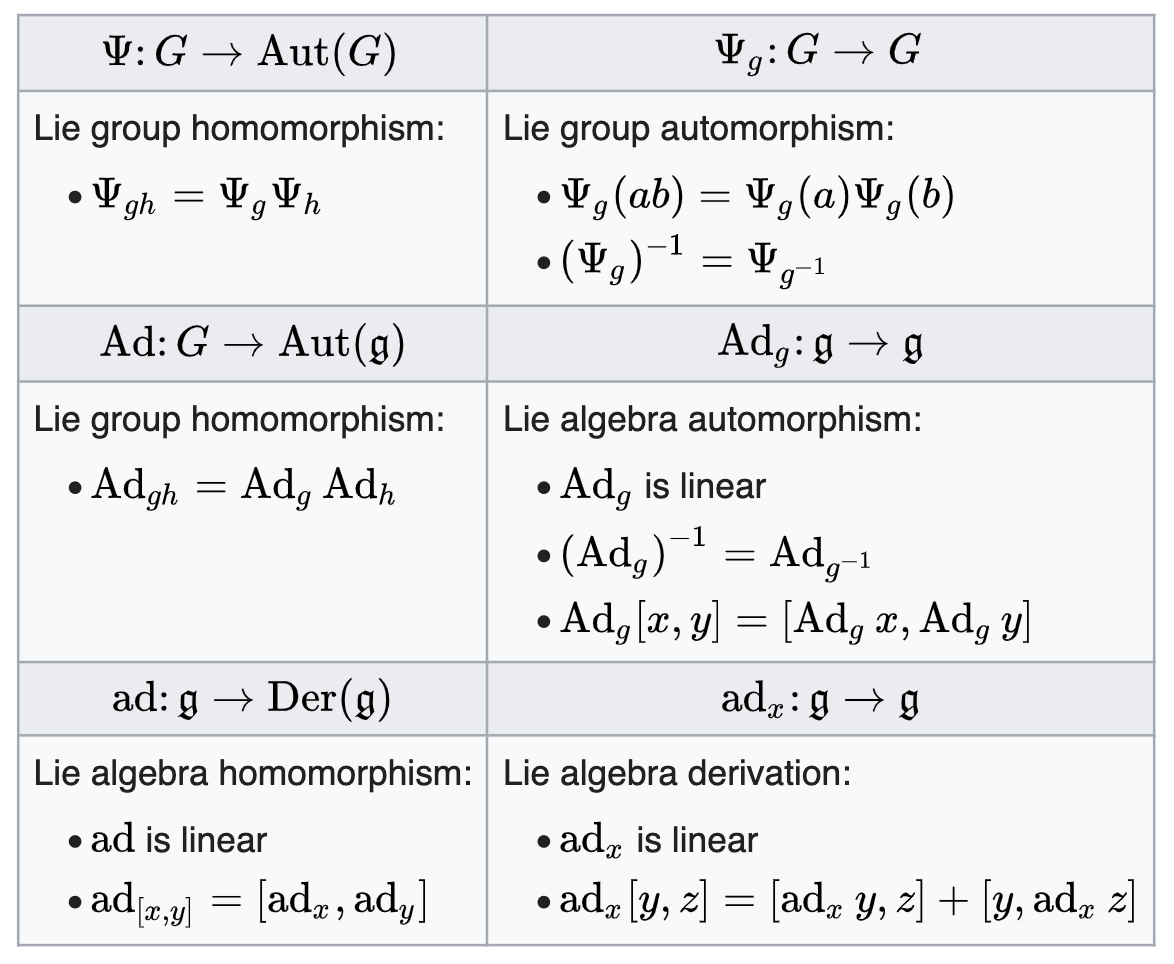
\includegraphics[scale=0.5]{Figs/adjoint.png}
    % \caption{Caption}
    % \label{fig:my_label}
\end{figure}

\end{enumerate}

















  




\section{Reconstruction of A Lie Group from Its Algebra: The Exponential Map}\label{sec:exp}
\adjustbox{center}{
\tikzset{LA/.style = {draw=red, % just to demonstrate, where LA is used
                      line width=#1,-{Straight Barb[length=3pt]}},
         LA/.default=1pt
        }
\begin{tikzcd}[row sep=0.5cm,column sep=0.5cm, color=black]
% b  & D\arrow[d,"\text{text}"] & b \\
\text{set} \arrow[r]& \text{topological space} \arrow[r] & \text{topological manifold} \arrow[r] & \text{differentiable manifold}\arrow[d] \arrow[r,""] & \text{principal fibre bundle}\arrow[r,""] & \text{associated fibre bundles} \\
& & &\text{Lie group}\arrow[d, xshift=0.7ex] \arrow[ru]  &&\\
& & &\text{Lie algebra}\arrow[u,LA,xshift=-0.7ex]    &&\\
\end{tikzcd}
}
A summary:
\begin{itemize}[$\blacktriangleright$]
\item
For any Lie group $G$, we could get Lie algebra $\mathcal{L}(G)\cong_\mathrm{Lie\, alg}T_eG\equiv \mathfrak{g}$. For the Lie algebra $\mathcal{L}(G)$, at least we could recover the $G$ of a \tb{neighbour around its identity $e$}. How large is the neighbour, the full $G$? It depends. Note, in this neighbour we have that the correspondence between the points on $G$ and the vector in $\mathcal{L}(G)$ is \tb{bijective} through the so called \tb{exponential map}.
\item We then state the \tb{one-to-one correspondence} between one-parameter subgroup, elements of the Lie algebra of the group and the left-invariant vector fields.
\end{itemize}

\begin{enumerate}
    \item \tb{integral curve:}  Let $M$ be a smooth manifold and let $Y\in \Gamma(TM)$. An \tb{integral curve} of $Y$ is smooth curve $\gamma\cl(-\varepsilon,\varepsilon)\to M$, with $\varepsilon > 0$, such that
\bse
\forall \, \lambda \in (-\varepsilon,\varepsilon) : \ X_{\gamma,\gamma(\lambda)} = Y|_{\gamma(\lambda)}.
\ese
\begin{itemize}
    \item \magenta{\tb{\green{local} existence and uniqueness of integral curve that pass a point:}} It follows from the \tb{local existence and uniqueness} of solutions to ordinary differential equations \cite{hartman2002ordinary} that, 
    \begin{itemize}[$\ast$]
        \item \tb{existence:} Given any $Y\in \Gamma(TM)$ and any $p\in M$, there \tb{exist} $\varepsilon >0$ and a \tb{smooth curve} $\gamma\cl (-\varepsilon,\varepsilon) \to M$ with \cyan{$\gamma(0)=p$} which is an \tb{integral curve} of $Y$. 
        \item \tb{uniqueness:} If $\gamma_1$ and $\gamma_2$ are both integral curves of $Y$ through $p$, i.e.\ $\gamma_1(0)=\gamma_2(0) = p$, then $\gamma_1=\gamma_2$ on the intersection of their domains of definition. 
        \item \tb{reparametrization?:}
        Given $\gamma(t)$, an integral curve of a vector field $Y$ on $M$, let $\hat{\gamma}(t):=\gamma(\sigma(t))$ be a reparametrized curve. \cyan{The only possible $\sigma(t)=t+\text{constant}$ that makes $\hat{\gamma}$ is still an integral curve of the vector field $Y$ is $\sigma(t)=t+\text{constant}$.}
{\tiny         
hint: $(d / d t) f(\gamma(\sigma(t)))=\sigma^{\prime}(t)(d / d t) f(\gamma(t))$, so that $\dot{\hat{\gamma}}=\sigma^{\prime} \dot{\gamma} ;[\sigma(t)=t+$ constant $]$.  $\hat{\gamma}$ is another trajectory, such that we traverse the same set of points on $M$ at different moments of time. At one point the new speed is $\sigma^{\prime}(t)$ times the old one at any point $\gamma(t)$.  Since the velocity vector of an integral curve may not be changed, $\sigma^{\prime}(t)=1$ is the only possible result. This means that the only possibility to change the trajectory is to traverse the same path either sooner or later.}
\item Let $\gamma$ be an integral curve of a vector field $Y$ on $M$, which starts from $P \equiv \gamma(0) \in M$. The integral curve (of the same field $Y$ ) $\hat{\gamma}$, which starts from $Q \equiv \gamma(a$ ), is $\hat{\gamma}(t):=\gamma(t+a)$
        
    \end{itemize}
    \item \tb{maximal integral curve:} The \tb{maximal integral curve} of $Y\in \Gamma(TM)$ through $p\in M$ is the \tb{unique integral curve} $\gamma\cl I^p_{\mathrm{max}}\to M$ of $Y$ through $p$, where
\bse
I_{\mathrm{max}}^{p} := \bigcup\{ I \se \R \mid \text{there exists an integral curve }\gamma\cl I \to M \text{ of $Y$ through $p$}\}.
\ese
\begin{itemize}[$\ast$]
    \item \tb{complete vector field:} A vector field is \tb{complete} if $I_{\mathrm{max}}^{p}=\R$ for all $p\in M$.
    \item \tb{compact $\Rightarrow$ complete:} On a \tb{compact} manifold, every vector field is \tb{complete}.
    \item \tb{left-invariant $\Rightarrow$ complete:} Every \tb{left-invariant} vector field on a Lie group is \tb{complete}. \teal{So we have a maximal integral curves of a left-invariant vector field. This is crucial in the construction of the map that allows us to go from a Lie algebra to a Lie group.}
    \item Example: See the ball in hairy ball theorem in \cref{sec:tensorII}. {\tiny Note the image of one curve may be not compact since we may never reach the point where the vector field vanishes. However, please note the theorem is talking about the domain manifold is compact. We still can get complete curves with the vector size become smaller and smaller if we move with $\lambda\rightarrow \infty$. With a \tb{non-compact} manifold, the field may suddenly vanishes and we cannot move any more.}
\end{itemize}
\item \orange{\tb{diffeomorphism  push-forward integral curve to integral curve:}} Recall in \cref{sec:cotangent} we mention the \tb{curve push-forward} under diffeomorphism. Now, if let $f: M \rightarrow M$ be a \tb{diffeomorphism} and let $\gamma(t)$ be the \tb{integral curve} of a field $Y$ which starts in $x \in M$. We have that the curve $f(\gamma(t))$ is then the \tb{integral curve} of the field $f_* Y$ which starts in $f(x)$.
\end{itemize}

\item \tb{exponential map:}  Let $G$ be a Lie group. Recall that given any $A\in T_eG$, we can define the uniquely determined \tb{left-invariant vector field} $K_A:=j(A)$ via the isomorphism $j\cl T_eG \xrightarrow{\sim}\mathcal{L}(G)$ as
\bse
K_A|_g := (\ell_g)_* (A).
\ese
Then let $\gamma^A\cl \R \to G$ be the \teal{\tb{maximal integral curve} of $K_A$ through $e\in G$}.  The \tb{exponential map} is defined as
\bi{rrCl}
\exp \cl & T_eG & \to & G\\
& A & \mapsto & \exp(A):=\gamma^A(1)
\ei
\begin{itemize}
\item \orange{\tb{comparison between $\exp$ and $j(A)$:}} The map $\exp$ is different from $j(A)$. It is we first select the $j(A)$ and then get the ``location'' at time 1. However, there is \tb{one to one correspondence} between them. See below one-parameter subgroup.
\begin{enumerate}
    \item They have \tb{range difference:}
\begin{itemize}[$\ast$]
\item The output of $j(\cdot)$ is a vector field while $\exp(\cdot)$ is a point on the manifold.
    \item In some sense, $j(\cdot)$ will cover the full $G$. This  is because left  translation $\ell_g$ is a \tb{diffeomorphism} on $G$. 
    \item However, for $\exp(\cdot)$, we will always travel from $e$, so it  can only reach the \tb{connected component} of $G$ containing the identity. See below for more details.
\end{itemize}
 \item Furthermore, as shown in \cref{sec:lie}, from the existence of global frame, we know that given any $X\in T_gG$, we can the find a unique $A \in T_eG$ such that $K_A|_g\equiv j(A)|_g=X$. But for $\exp$ we only have the following \tb{local diffeomorphism} in general.
\end{enumerate}

    \item \tb{local diffeomorphism:} The map $\exp$ is smooth and a \tb{local diffeomorphism} around $0\in T_eG$, i.e.\ there exists an open set $U\se T_eG$ containing $0$ such that the restriction
\bse
\exp|_U\cl U \to \exp(U) \se G
\ese
is \tb{bijective} and both $\exp|_U$ and $(\exp|_U)^{-1}$ are \tb{smooth}.
\begin{itemize}[$\ast$]
    \item Note that the maximal integral curve of $X^0$ is the constant curve $\gamma^0(\lambda)\equiv e$, and hence we have $\exp(0)=e$. It means that we can \cyan{recover a {\tb{neighbourhood}} of the identity of $G$ from a neighbourhood of the identity of $T_eG$.} 
\end{itemize}

\item \tb{How large is $\exp(T_eG)$?:} Let $G$ be a Lie group. We can only say that the image of $\exp\cl T_eG\to G$ is  \cyan{a subset of the \tb{connected component} of $G$ containing the identity.} In some cases, $\exp$ is  \tb{surjective} so that the \cyan{neighbor is the full $G$}. 
    \begin{enumerate}%[$\$]
        \item $G$ is connected and compact. {\tiny Since $T_eG$ is a vector space, it is non-compact. Hence, if $G$ is compact, $\exp$ cannot be injective. This is because diffeomorphism will keep the compactness.}
\item $G$ is connected and nilpotent (for example, $G$ connected and abelian).
\item 
$ G=\GL_{n}({\mathbb{C}})$.
    \end{enumerate}
\begin{itemize}[$\ast$]
\item Example: {\tiny Let $B\cl V\times V$ be a pseudo inner product on $V$. Then recall that
\bse
\Ort(V) := \{\phi\in \GL(V)\mid \forall \, v,w\in V : B(\phi(v),\phi(w))=B(v,w)\}
\ese
is called the \tb{orthogonal group} of $V$ with respect to $B$. Every $\phi\in \Ort(V)$ has determinant $1$ or $-1$. Since $\det$ is multiplicative, we have a \tb{subgroup}
\bse
\SO(V) := \{\phi\in \Ort(V)\mid \det\phi = 1\}.
\ese
These are, in fact, Lie subgroups of $\GL(V)$. The Lie group $\SO(V)$ is connected while
\bse
\Ort(V)=\SO(V)\cup \{\phi\in \Ort(V)\mid \det \phi = -1\}
\ese
is disconnected. Since $\SO(V)$ contains $\id_V$, we have
\bse
\so(V) := T_{\id_V}\!\SO(V) = T_{\id_V}\!\Ort(V) =: \ort(V)
\ese
and
\bse
\exp(\so(V))=\exp(\ort(V))=\SO(V).
\ese
where $\so(V)$ is the Lie algebra associated with Lie group $\SO(V)$.}
\end{itemize}

\item \tb{parameterization of $G$ near $e$:} Because of the \tb{diffeomorphism} (especially bijective), choosing a basis $A_1,\ldots,A_{\dim G}$ of $T_eG$ provides a convenient parameterization in the form of $\exp(\lambda^iA_i)$ for the points in the neighbor $U$ mentioned above in $G$ near $e$.

\begin{itemize}[$\ast$]
    \item Example: {\tiny 
 Consider, for example, the \tb{Lorentz group}
\bse
\Ort(3,1) \equiv \Ort(\R^4) = \{\Lambda\in \GL(\R^4)\mid \forall \, x,y\in \R^4 :  B(\Lambda(x),\Lambda(y))=B(x,y) \},
\ese
where $B(x,y):=\varepsilon_{\mu\nu}x^\mu y^\nu$, with $0\leq \mu,\nu\leq 3$ ($x^\mu$ is the components of x) and
\bse
[\varepsilon^{\mu\nu}] = [\varepsilon_{\mu\nu}] := \left( 
  \begin{matrix}
  -1 & 0 & 0 & 0 \\
    0 & 1 & 0 & 0 \\
    0 & 0 & 1 & 0 \\
    0 & 0 & 0 & 1
  \end{matrix}\right).
\ese
The Lorentz group $\Ort(3,1)$ is $6$-dimensional, hence so is the \tb{Lorentz algebra} $\ort(3,1)$. For convenience, instead of denoting a basis of $\ort(3,1)$ as $\{M^i\mid i=1,\ldots,6\}$, we will denote it as $\{M^{\mu\nu}\mid 0\leq \mu,\nu\leq 3\}$ and require that the indices $\mu,\nu$ be anti-symmetric, i.e.\
\bse
M^{\mu\nu} = -M^{\nu\mu }.
\ese
Then $M^{\mu\nu}=0$ when $\rho=\sigma$, and the set $\{M^{\mu\nu}\mid 0\leq \mu,\nu\leq 3\}$, while technically not linearly independent, contains the 6 independent elements that we want to consider as a basis. These basis elements satisfy the following bracket relation
\bse
[M^{\mu\nu},M^{\rho\sigma}] =\eta^{\nu\sigma} M^{\mu\rho} +\eta^{\mu\rho} M^{\nu\sigma} -\eta^{\nu\rho} M^{\mu\sigma} -\eta^{\mu\sigma} M^{\nu\rho} . 
\ese
Any element $\lambda\in \ort(3,1)$ can be expressed as linear combination of the $M^{\mu\nu}$,
\bse
\lambda = \tfrac{1}{2}\omega_{\mu\nu}M^{\mu\nu}
\ese
where the indices on the coefficients $\omega_{\mu\nu}$ are also anti-symmetric, and the factor of $\tfrac{1}{2}$ ensures that the sum over all $\mu,\nu$ counts each anti-symmetric pair only once. Then, we have
\bse
\Lambda = \exp(\lambda) = \exp(\tfrac{1}{2}\omega_{\mu\nu}M^{\mu\nu}) \in \Ort(3,1).
\ese
The subgroup of $\Ort(3,1)$ consisting of the the space-orientation preserving Lorentz transformations, or \emph{proper} Lorentz transformations, is denoted by $\SO(3,1)$. The subgroup consisting of the time-orientation preserving, or \emph{orthochronous}, Lorentz transformations is denoted by $\Ort^+(3,1)$. The Lie group $\Ort(3,1)$ is disconnected: its \tb{four connected components} from which we care about the connected component $\SO^+(3,1):=\SO(3,1)\cap\Ort^+(3,1)$, also called the \emph{restricted Lorentz group}, consisting of the proper orthochronous Lorentz transformations;
Since $\id_{\R^4}\in \SO^+(3,1)$, we have $\exp(\ort(3,1))=\SO^+(3,1)$. Then $\{M^{\mu\nu}\}$ provides a nice \tb{parameterization} of $\SO^+(3,1)$ since, if we choose
\bse
[\omega_{\mu\nu}] = \left(
  \begin{matrix}
        0   &   \psi_1   &   \psi_2   &   \psi_3   \\
    -\psi_1 &      0     &  \varphi_3 & -\varphi_2 \\
    -\psi_2 & -\varphi_3 &      0     &  \varphi_1 \\
    -\psi_3 &  \varphi_2 & -\varphi_1 &      0
  \end{matrix}
\right)
\ese
then the Lorentz transformation $\exp(\tfrac{1}{2}\omega_{\mu\nu}M^{\mu\nu})\in \SO^+(3,1)$ corresponds to a boost in the $(\psi_1,\psi_2,\psi_3)$ direction and a space rotation by $(\varphi_1,\varphi_2,\varphi_3)$. Indeed, in physics one often thinks of the Lie group $\SO^+(3,1)$ as being generated by $\{M^{\mu\nu}\}$.

A \tb{representation of the Lie algebra is} $\rho\cl T_{\id_{\R^4}}\!\SO^+(3,1)\xrightarrow{\sim} \End(\R^4)$ is given by
\bse
\rho(M^{\mu\nu})^a_{\phantom{a}b} := \eta^{\nu a}\delta^{\mu}_b - \eta^{\mu a}\delta^{\nu}_b 
\ese
which is probably how you have seen the $M^{\mu\nu}$ themselves defined in some previous course on relativity theory. \cyan{Using this representation, we get a corresponding representation}
\bi{rrCl}
R\cl & \SO^+(3,1) \to \GL(\R^4)
\ei
via the exponential map by defining
\bse
R(\Lambda) = \exp(\tfrac{1}{2}\omega_{\mu\nu}\rho(M^{\mu\nu})).
\ese
Then, the map $\exp$ becomes the usual exponential (series) of matrices.}
\end{itemize}
\end{itemize}

\item \tb{one-parameter subgroup:} A \tb{one-parameter subgroup} of a Lie group $G$ is a \tb{Lie group homomorphism}
\bse
\xi \cl \R \to G,
\ese
with \cyan{$\R$ understood as a Lie group under ordinary addition ``$+$''.} In other words, $$\gamma(t+s)=\gamma(t) \gamma(s) \quad \gamma(0)=e \quad t, s \in \mathbb{R}.$$

We next state some facts:
\begin{itemize}
    \item Denote $K_A\in \calL(G)$ as the \tb{left-invariant vector field} on $G$ which is generated by a vector $A \in \mathfrak{g}\equiv T_eG$.
    \begin{enumerate}
        \item Its \tb{integral curve} $\gamma^A(t)$ starting from $e$ is a \tb{oneparameter subgroup} since we have
$$ \gamma^A(t+s)=\gamma^A(t) \gamma^A(s) \quad \gamma^A(0)=e.$$
{\scriptsize hint: the curve $\Gamma(t):=\gamma^A(t+s)$ is the integral curve of $K_A$ starting at $\gamma^A(s)$. Since $L_{g *} K_A=K_A$ for any $g$ as $K_A$ is left-invariant, the curve $\Gamma(t)$ is also the integral curve of the field $L_{\gamma^A(s) *} K_A$. Note, by the push-forward, the integral curve of $L_{\gamma^A(s) *}K_A$ is $\gamma^A(s) \gamma^A(t)$. Put together $\gamma^A(t+s)=$ $\gamma^A(t) \gamma^A(s)$.}

\item If, in turn, $\gamma(t)$ is an arbitrary \tb{one-parameter subgroup},
then it is necessarily the \tb{integral curve of the left-
invariant field $K_A$} with $A \equiv K_A(e)=\dot{\gamma}(0)$. The complete trajectory $\gamma(t)$ then turns out to be \tb{determined by its initial velocity}, i.e. by the tangent vector $\dot{\gamma}(0)=A$ at the
starting point $e.$

{\tiny hint: we have
\begin{align*}
\begin{aligned}
\dot{\gamma}(t) &=\left.\frac{d}{d s}\right|_{s=0} \gamma(t+s)=\left.\frac{d}{d s}\right|_0 \gamma(t) \gamma(s)=\left.\frac{d}{d s}\right|_0 L_{\gamma(t)} \gamma(s)=\left.L_{\gamma(t) *} \frac{d}{d s}\right|_0 \gamma(s)=L_{\gamma(t) *} X \\
&=K_A(\gamma(t))
\end{aligned}
\end{align*}}
    \end{enumerate}
    \item Since we have the correspondence $A\Leftrightarrow\gamma^A(t)\Leftrightarrow K_A$, there is a \tb{one-to-one correspondence:}
    \begin{figure}[H]
        \centering
       \begin{tikzcd}[color=magenta]
\text{elements of the Lie algebra of the group} \arrow[r, Leftrightarrow] & \text{one-parameter subgroups} \arrow[r, Leftrightarrow] & \text{left-invariant vector fields}
\end{tikzcd}
    \end{figure}
    \item The one-parameter subgroup satisfies
\begin{align*}
\gamma^X(k t)=\gamma^{k X}(t) \quad k \in \mathbb{R}
\end{align*}
since they have the same initial velocity. This enables one to express the one-parameter subgroup in terms of an exponential map in the form
\begin{align*}
\gamma^X(t)=\exp t X \equiv e^{t X}
\end{align*}

\item \tb{explicit form on $\GL(n, \mathbb{R})$:} Using \cite{fecko2006differential}[11.1.10], the local representation of left-invariant vector fields of $\GL(n, \mathbb{R})$, we have the equation
$$\dot{x}(t)=x(t) C, x(0)=\mathbb{I}_n.$$
The solution of this (matrix) equation is
\begin{align*}
x(t)=\exp t C \equiv e^{t C}:=\mathbb{I}_n+t C+\frac{t^2}{2 !} C^2+\cdots
\end{align*}
\end{itemize}

\item \tb{exponential map under Lie group homomorphism:} Let $G$ and $H$ be Lie groups and let $\phi\cl G \to H$ be a \tb{Lie group homomorphism}. Then, for all $A\in T_{e_G}G$, we have
\bse
\phi (\exp (A))= \exp ((\phi_*)_{{\scriptstyle e}_G}A).
\ese
\begin{itemize}
    \item \tb{equivalent statement:} the following diagram commutes.
\bse
\begin{tikzcd}
T_{e_G}G \ar[dd,"\exp"'] \ar[rr,"(\phi_*)_{{\scriptstyle e}_G}"]&& T_{e_H}H\ar[dd,"\exp"]\\
&&\\
G\ar[rr,"\phi"] && H
\end{tikzcd}
\ese
\item \tb{Adjoint map and exponential map:}
In particular, for $\phi\equiv \Ad_g\cl G\to G$, we have
\bse
\Ad_g (\exp(A)) = \exp(({\Ad_g}_*)_eA).
\ese
\end{itemize} 




\end{enumerate}





\section{Principal Fibre Bundles}\label{sec:principal}
\adjustbox{center}{
\tikzset{LA/.style = {draw=red, % just to demonstrate, where LA is used
                      line width=#1,-{Straight Barb[length=3pt]}},
         LA/.default=1pt
        }
\begin{tikzcd}[row sep=0.5cm,column sep=0.5cm, color=black]
% b  & D\arrow[d,"\text{text}"] & b \\
\text{set} \arrow[r]& \text{topological space} \arrow[r] & \text{topological manifold} \arrow[r] & \text{differentiable manifold}\arrow[d] \arrow[r,,LA,""] & \text{principal fibre bundle}\arrow[r,""] & \text{associated fibre bundles} \\
& & &\text{Lie group}\arrow[d, xshift=0.7ex] \arrow[ru,LA]  &&\\
& & &\text{Lie algebra}\arrow[u,xshift=-0.7ex]    &&\\
\end{tikzcd}
}
Very roughly speaking, \teal{a principal fibre bundle is a bundle whose typical fibre is a Lie group.} Principal fibre bundles are so immensely important because they allow us to understand any fibre bundle with fibre $F$ on which a Lie group $G$ acts. These are then called associated fibre bundles, and will be discussed later on.

A summary:
\begin{itemize}[$\blacktriangleright$]
\item We first introduce the \tb{left and right Lie group action $G$ on manifold $M$}. The concept of \tb{orbit} as equivalence relation on $M$ and \tb{stabiliser} as subgroup $G$ are then defined.
\item We then introduce \tb{principal fibre bundles} from the above  equivalence classes from a \tb{free action}.
\item The \tb{frame bundle} is then introduced in detail.
\item We state the \tb{principal bundle morphisms} which requires the extra \tb{{$\rho$-equivariant}} condition besides the bundle morphism condition.
\item Finally, we state the \tb{restriction and extension} of principal fibre bundles in terms of Lie subgroup.
\end{itemize}

\begin{enumerate}
    \item \tb{left group action:} Let $(G,\bullet)$ be a Lie group and let $M$ be a smooth manifold. A smooth map
\bi{rrCl}
\lacts \cl & G\times M & \to & M\\
& (g,p) & \mapsto & g \lacts p
\ei
satisfying
\begin{enumerate}
    \item \item $\forall \, p \in M :\ e\lacts p = p$;
\item $\forall \, g_1,g_2\in G : \forall \, p\in M : \ (g_1\bullet g_2) \lacts p = g_1 \lacts (g_2 \lacts p)$,
\end{enumerate}

is called a \tb{left Lie group action}, or \tb{left $G$-action}, on $M$. 
\begin{itemize}
    \item \tb{left $G$-manifold:} A manifold equipped with a left $G$-action is called a \tb{left $G$-manifold}.
    \item  The smooth structures on $G$ and $M$ were only used in the requirement that $\lacts$ be smooth. By dropping this condition, we obtain the usual definition of a group action on a set. So concepts like \tb{orbits} and \tb{stabilisers} can then be defined.
    \item Example:  Let $G$ be a Lie group and let $R\cl G \to \GL(V)$ be a \tb{representation} of $G$ on a vector space $V$. Define a map
\bi{rrCl}
\lacts \cl & G \times V & \to & V\\
& (g,v) & \mapsto & g\lacts v := R(g)v.
\ei
We easily check that $e\lacts v := R(e)v = \id_V v = v$ and
\bi{rCl}
(g_1\bullet g_2) \lacts v & := & R(g_1\bullet g_2)v\\
& = & (R(g_1)\circ R(g_2))v\\
& = & R(g_1)( R(g_2)v)\\
& = & g_1 \lacts (g_2 \lacts v),
\ei
for any $v\in V$ and any $g_1,g_2\in G$. 
\begin{itemize}[$\ast$]
    \item  In some sense, we can therefore think of left $G$-actions as ``generalised'' representations of $G$ on some manifold.
\end{itemize}
\end{itemize}

\item \tb{right $G$-action:}
Similarly, a \tb{right $G$-action} on $M$ is a smooth map
\bi{rrCl}
\racts \cl & M\times G & \to & M\\
& (p,g) & \mapsto & p \racts g
\ei
satisfying
\begin{enumerate}
  \item $\forall \, p \in M :\ p\racts g = p$;
\item $\forall \, g_1,g_2\in G : \forall \, p\in M : \ p \racts (g_1\bullet g_2) = (p \racts g_1) \racts g_2$.
\end{enumerate}

\begin{itemize}
    \item \tb{from left to right action:} Let $\lacts$ be a left $G$-action on $M$. Then
\bi{rrCl}
\racts \cl & M\times G & \to & M\\
& (p,g) & \mapsto & p \racts g := g^{-1} \lacts p
\ei
is a right $G$-action on $M$.
\item In some sense, left and right action are dual. But later, within the context of \tb{principal and associated fibre bundles}, we will attach \tb{separate} ``meanings'' to left and right actions.  See \cref{sece:asso}.
\item \tb{change of basis viewed from Lie group actions:} {\tiny  Recall that if we have a basis $e_1,\ldots,e_{\dim M}$ of $T_pM$ and $X^1,\ldots,X^{\dim M}$ are the components of some $X\in T_pM$ in this basis, then under a change of basis
\bse
\widetilde e_a = A^b_{\phantom{b}a}e_b,
\ese
we have $X=\widetilde X^a \widetilde e_a$, where
\bse
\widetilde X^a = (A^{-1})^a_{\phantom{a}b}X^b.
\ese
Once expressed in terms of principal and associated fibre bundles, we will see that the ``recipe'' of labelling the basis by lower indices and the vector components by upper indices, as well as their transformation law, can be understood as a \tb{right action} of $\GL(\dim M, \R)$ on the basis and a \tb{left action} of the same $\GL(\dim M, \R)$ on the components.} See \cref{sece:asso} for more details.
\end{itemize}

\item \tb{{$\rho$-equivariant}:} Let $G,H$ be Lie groups, let $\rho\cl G\to H$ be a Lie group homomorphism and let
\bi{l}
\lacts \cl G \times M \to M,\\
\blacktriangleright \cl H \times N \to N
\ei
be left actions of $G$ and $H$ on some smooth manifolds $M$ and $N$, respectively. Then, a smooth map $f\cl M\to N$ is said to be \blue{\tb{$\rho$-equivariant}} if the diagram
\bse
\begin{tikzcd}
G\times M \ar[dd,"\lacts"'] \ar[rr,"\rho\times f"]&& H\times N \ar[dd,"\blacktriangleright"]\\
&&\\
M \ar[rr,"f"] && N
\end{tikzcd}
\ese
where $(\rho\times f)(g,p) := (\rho(g),f(p))\in H\times N$, commutes. Equivalently,
\bse
\forall \, g \in G : \forall \, p \in M : \ f(g\lacts p) = \rho(g)\blacktriangleright f(p).
\ese
\begin{itemize}
    \item $\rho$-equivariant maps are the ``action-preserving'' maps between the $G$-manifold $M$ and the $H$-manifold $N$.
     \item \tb{equivalent diagram representation:} We sometime draw it in the following form\bse
     \begin{tikzcd}
M \ar[rr,"u"]&& N \\
&&\\
G\times M\ar[uu,"{}\lacts "]  \ar[rr,"\rho\times f"]&& H\times N \ar[uu,"{}\blacktriangleright"'] \\
&&\\
M \ar[uu,"i_1"]  \ar[rr,"f"] && N\ar[uu,"i_1"'] \\
\end{tikzcd}
\ese
     
    \item If $\rho = \id_G$ or $f=\id_M$, the notion of $f$ being $\rho$-equivariant reduces to
    \begin{itemize}[$\ast$]
        \item $\rho = \id_G$:  \blue{homomorphism of $G$-manifolds} as  $f(g\lacts p) = g\blacktriangleright f(p).$ In this case, we may suppress the above diagram to the following
        \bse
\begin{tikzcd}
M \ar[rr,"u"]&& N \\
&&\\
M \ar[uu,"{}G\lacts "]  \ar[rr,"u"] && N\ar[uu,"{}G\blacktriangleright "']\\
\end{tikzcd}
\ese
        Note that $M\xrightarrow{\quad G\lacts  \quad } P$ is a shorthand for the inclusion of $M$ into the product $G\times M$ followed by the left action $\lacts$, i.e.\
\bse
\begin{tikzcd}
M\ar[rr,"G\lacts "] && M
\end{tikzcd}
\ \quad =\quad \ 
\begin{tikzcd}
M \ar[rr,"i_1"] && G\times M \ar[rr,"\lacts"] && M
\end{tikzcd}
\ese
        \item $f=\id_M$:  homomorphism of left actions on $M$ as  $g\lacts p = \rho(g)\blacktriangleright p.$
    \end{itemize}
\end{itemize}
\item \tb{orbit:} Let $\lacts \cl G \times M \to M$ be a left $G$-action. For each $p\in M$, we define the \tb{orbit} of $p$ as the set
\bse
G_p :=\{q\in M\mid \exists \, g\in G : q = g\lacts p\}.
\ese

\begin{itemize}
    \item Alternatively, the orbit of $p$ is the image of $G$ under the map $( {}-\lacts p)$. 
   \item \tb{orbit as equivalence class:}
Let $\lacts \cl G\times M \to M$ be an action on $M$. Define a relation on $M$
\bse
p\sim q \ :\Leftrightarrow \ \exists \, g \in G : q = g \lacts p.
\ese
Then $\sim$ is an \tb{equivalence relation} on $M$.
\item \tb{orbit space as quotient space:} Let $\lacts\cl G\times M\to M$ be an action on $M$. The \tb{orbit space} of $M$ is
\bse
\green{M/G} := M/\!\sim \,= \{G_p \mid p\in M\}.
\ese
\item \tb{transitive:} A left $G$-action $\lacts\cl G\times M\to M$ is said to be
\tb{transitive} if for all $p,q\in M$, there exists $g\in G$ such that $p=g\lacts p$.
\begin{itemize}[$\ast$]
    \item Note, $G$ always acts \tb{transitively} on $G_p$.
\end{itemize}
    \item Example: Consider the action induced by representation of $\SO(2,\R)$ as rotation matrices in $\End(\R^2)$. The orbit of any $p\in\R^2$ is the circle of radius $|p|$ centred at the origin.
\begin{center}
\begin{tikzpicture}[scale=0.8]
\draw[gray,->] (0,-4) -- (0,4);
\draw[gray,->] (-4,0) -- (4,0);
\draw (3.25,3.25) node {$\R^2$};
\draw[dashed] (0,0) -- (1.75*cos 40 , 1.75*sin 40) node[above right] {$p$};
\draw[fill] (1.75*cos 40 , 1.75*sin 40) circle[radius=0.05];
\draw (1.75*cos -40 , 1.75*sin -40) node[below right=-2pt] {$G_p$};
\draw (-0.1+0.8*cos 40 , 0.8*sin 40) node[above=3pt] {$|p|$};
\draw[dashed] (0,0) -- (2.9*cos 140 , 2.9*sin 140) node[above left] {$q$};
\draw[fill] (2.9*cos 140 , 2.9*sin 140) circle[radius=0.05];
\draw (2.9*cos -50 , 2.9*sin -50) node[below right=-2pt] {$G_q$};
\draw(1*cos 140 , 1*sin 140) node[above=4pt ] {$|q|$};
\draw[semithick] (0,0) circle [radius=1.75];
\draw[semithick] (0,0) circle [radius=2.9];
\draw[fill] (0,0) circle [radius=0.05] node[below right] {$G_0$};
\draw(0,0)  node[below left] {$0$};
\end{tikzpicture}
\end{center}
The orbit space  the partition of $\R^2$ into concentric circles centred at the origin, plus the origin itself. So $\SO(2,\R)$ is \tb{not} transitive on $\R^2$. However, we can say it is \tb{transitive} on the  circles!
\end{itemize}

\item \tb{stabiliser:}
Let $\lacts\cl G\times M\to M$ be a $G$-action on $M$. The \tb{stabiliser} of $p\in M$ is
\bse
S_p:=\{g\in G\mid g\lacts p = p\}.
\ese
\begin{itemize}
    \item Note that for each $p\in M$, the stabiliser $S_p$ is a \tb{subgroup} of $G$. 
    \item A left $G$-action $\lacts\cl G\times M\to M$ is said to be
   \cyan{\tb{free}} if \purple{for all} $p\in M$, we have $S_p=\{e\}$.

\item \tb{stabiliser and orbit relation:} We have the following \tb{bijection} $\phi$ \begin{align*}
\begin{aligned}
\phi: G / S_p & \rightarrow G_p \\
g S_p & \mapsto g\lacts p
\end{aligned}
\end{align*}where $gS_p\coloneqq \{g\bullet h| h\in S_p\}$ is a equivalent class called left coset induced from the subgroup (See my algebra notes).
    \item Let $\lacts\cl G \times M \to M$ be a \tb{free action}. Then
\bse
g_1 \lacts p = g_2 \lacts p \quad \Leftrightarrow \quad g_1 = g_2.
\ese
That means \cyan{under free action, we have a one to one map between $G$ and the orbit $S_p$ for any point $p$ on the manifold.} \magenta{Furthermore, $\lacts\cl G \times M \to M$ is a \tb{free} action, then
\bse
\forall \, p \in G :\ G_p \cong_{\mathrm{diff}} G.
\ese}
\item For \tb{right} action, the above definitions and conclusions also follow analogously.
\item Examples: 
\begin{itemize}[$\dagger$]
    \item The action $\lacts\cl G\times V \to V$ induced by a representation $R\cl G\to \GL(V)$ is never free since we always have $S_0=G$.
    \item Consider the action $\lacts\cl \mathrm{T}(n)\times \R^n\to \R^n$ of the $n$-dimensional translation group $\mathrm{T}(n)$ on $\R^n$. We have $\mathrm{T}(n)_p=\R^n$ for every $p\in \R^n$, a subjective. It is also easy to show that this action is free and transitive. 
    \item Define $\lacts\cl \SO(2,\R)\times \R^2\purple{\sm\{0\}}\to \R^2\purple{\sm\{0\}}$ to coincide with the action induced by the representation of $\SO(2,\R^2)$ on $\R^2$ for each non-zero point of $\R^2$. Then this action is \tb{free}, since we have $S_p=\{\id_{\R^2}\}$ for $p\neq 0$, and the previous proposition implies
\bse
\forall \, p\in \R^2\sm\{0\} : \ \SO(2,\R)_p \cong_{\mathrm{diff}} \SO(2,\R) \cong_{\mathrm{diff}} S^1.
\ese
\end{itemize}


\end{itemize}

\item \orange{\tb{principal $G$-bundle:}}
Let $G$ be a Lie group. A smooth bundle $(E,\pi,M)$ is called a \tb{principal $G$-bundle} \orange{if $E$ is equipped with a \tb{\magenta{free} right $G$-action}} and
\bse
\begin{tikzcd}
E \ar[d,"\pi"'] \\
M 
\end{tikzcd}
\ \ \cong_{\mathrm{bdl}}
\begin{tikzcd}
  E \ar[d,"\rho"]\\
 \green{ E/G}
\end{tikzcd}
\ese
where $\rho$ is the \tb{quotient map}, defined by sending each $p\in E$ to its equivalence class (i.e.\ orbit) in the orbit space $E/G$.

\begin{itemize}
    \item Since the right action of $G$ on $E$ is \tb{free}, for each $p\in E$ we have
\magenta{\bse
\preim_\rho(G_p) \cong_{\mathrm{diff}} G_p \cong_{\mathrm{diff}} G.
\ese}
So roughly speaking, \teal{a principal bundle is a bundle whose fibre at each point is a Lie group.}
\item A principal $G$-bundle is a bundle which is \tb{isomorphic} to a bundle whose \tb{\teal{fibres are the orbits}} under the right action of $G$, which are themselves \tb{\teal{isomorphic to $G$}} since the action is free.
\item The isomorphism in our definition enforces the \tb{fibre-wise transitivity} since $G$ acts transitively on each $G_p$ by the definition of orbit.
\end{itemize}


\item \cyan{\tb{frame bundle:}} We now define the frame bundle using \tb{principal $G$-bundle}.
\begin{enumerate}

\item Let $M$ be a smooth manifold. Consider the space
\bse
L_pM := \{(e_1,\ldots,e_{\dim M})\mid e_1,\ldots,e_{\dim M} \text{ is a basis of }T_pM\} \cong_{\mathrm{vec}} \GL(\dim M,\R).
\ese
We define the frame bundle of $M$ as
\bse
LM := \coprod_{p\in M} L_pM
\ese
with the obvious projection map $\pi\cl LM \to M$ sending each basis $(e_1,\ldots,e_{\dim M})$ to the unique point $p\in M$ such that $(e_1,\ldots,e_{\dim M})$ is a basis of $T_pM$.
{\tiny \begin{itemize}
    \item By proceeding similarly to the case of the tangent bundle, we can equip $LM$ with a smooth structure inherited from that of $M$. We then find
\bse
\dim LM = \dim M + \dim T_pM = \dim M + (\dim M)^2.
\ese
\end{itemize}}


\item We would now like to make $LM \xrightarrow{\,\pi\,}M$ into a \cyan{principal $\GL(\dim M,\R)$-bundle.} We define a right $\GL(\dim M,\R)$-action on $LM$ by
\bse
(e_1,\ldots,e_{\dim M}) \racts g := (g^a_{\phantom{a}1}e_a,\ldots,g^a_{\phantom{a}\dim M}e_a),
\ese
where $g^a_{\phantom{a}b}$ are the components of the endomorphism $g\in \GL(\dim M, \R)$ with respect to the standard basis on $\R^n$.
\begin{itemize}
    \item Note that if $(e_1,\ldots,e_{\dim M})\in L_pM$, we must also have $(e_1,\ldots,e_{\dim M}) \racts g\in L_pM$.
    \item This action is \tb{free} since
\bse
(e_1,\ldots,e_{\dim M}) \racts g = (e_1,\ldots,e_{\dim M})  \Leftrightarrow  (g^a_{\phantom{a}1}e_a,\ldots,g^a_{\phantom{a}\dim M}e_a)= (e_1,\ldots,e_{\dim M}) 
\ese and hence, by linear independence, $g^a_{\phantom{a}b}=\delta^a_b$, so $g=\id_{\R^n}$.
\item Note that since all bases of each $T_pM$ are related by some $g\in \GL(\dim M,\R)$, $\racts$ is also \tb{fibre-wise transitive}. 
\end{itemize} 
\item We now have to show that
\bse
\begin{tikzcd}
LM \ar[d,"\pi"'] \\
M 
\end{tikzcd}
\ \ \cong_{\mathrm{bdl}}
\begin{tikzcd}
  LM \ar[d,"\rho"]\\
  LM \big/ \GL(\dim M,\R)
\end{tikzcd}
\ese
i.e.\ that there exist smooth maps $u$ and $f$ such that the diagram
\bse
\begin{tikzcd}
LM \ar[rr,shift left,"u"] \ar[dd,"\pi"']&& LM \ar[ll,shift left,"u^{-1}"]\ar[dd,"\rho"]\\
&&\\
M \ar[rr,shift left,"f"]&&  LM \big/ \GL(\dim M,\R)\ar[ll,shift left,"f^{-1}"]
\end{tikzcd}
\ese
commutes. We can simply choose $u=u^{-1}=\id_{LM}$, while we define $f$ as
\bi{rrCl}
f \cl & M & \to &  LM\big/ \GL(\dim M,\R)\\[2pt]
& p & \mapsto & \GL(\dim M,\R)_{(e_1,\ldots,e_{\dim M})},
\ei
where $(e_1,\ldots,e_{\dim M})$ is some basis of $T_pM$, i.e.\ $(e_1,\ldots,e_{\dim M})\in \preim_\pi(\{p\})$.   $LM\xrightarrow{\,\pi\,}M$ is a principal $G$-bundle, called the \cyan{\tb{frame bundle}} of $M$.
\begin{itemize}
    \item Note that $f$ is \tb{well-defined} since every basis of $T_pM$ gives rise to the same orbit in the orbit space $LM\big/\GL(\dim M,\R)$. 
    {\tiny \begin{itemize}[$\ast$]
        \item 
   Moreover, it is \tb{injective} since
\bse
f(p)=f(p')\ \Leftrightarrow \ \GL(\dim M,\R)_{(e_1,\ldots,e_{\dim M})} = \GL(\dim M,\R)_{(e'_1,\ldots,e'_{\dim M})},
\ese
which is true only if $(e_1,\ldots,e_{\dim M})$ and $(e'_1,\ldots,e'_{\dim M})$ are basis of the same tangent space, so $p=p'$.
\item 
 It is clearly \tb{surjective} since every orbit in $LM\big/ \GL(\dim M,\R)$ is the orbit of some basis of some tangent space $T_pM$ at some point $p\in M$. 
 \end{itemize}}
 \item The \tb{inverse} map is given explicitly by
\bi{rrCl}
f^{-1} \cl & LM\big/ \GL(\dim M,\R) & \to & M \\[2pt]
& \GL(\dim M,\R)_{(e_1,\ldots,e_{\dim M})} & \mapsto & \pi((e_1,\ldots,e_{\dim M})).
\ei
\item 
Finally, we have
\bse
(\rho\circ\id_{LM})(e_1,\ldots,e_{\dim M}) = \GL(\dim M,\R)_{(e_1,\ldots,e_{\dim M})} = (f\circ \pi)(e_1,\ldots,e_{\dim M})
\ese
and thus $LM\xrightarrow{\,\pi\,}M$ is a principal $G$-bundle, called the \tb{frame bundle} of $M$.
\end{itemize}
\end{enumerate}
\item 
\tb{principal bundle morphisms:}{\tiny
Recall that a bundle morphism (also called simply a bundle map) between two bundles $(E,\pi,M)$ and $(E',\pi',M')$ is a pair of maps $(u,f)$ such that the diagram
\bse
\begin{tikzcd}
E \ar[dd,"\pi"'] \ar[rr,"u"] && E' \ar[dd,"\pi'"]\\
&&\\
M\ar[rr,"f"] && M'
\end{tikzcd}
\ese
commutes, that is, $f\circ \pi = \pi' \circ u$.}
Let $(P,\pi,M)$ and $(Q,\pi',N)$  \cyan{both be principal $G$-bundles}. A \tb{principal bundle morphism} from $(P,\pi,M)$ to $(Q,\pi',N)$ is a pair of smooth maps $(u,f)$ such that the diagram
\bse
\begin{tikzcd}
P \ar[rr,"u"]&& Q \\
&&\\
P \ar[uu,"{}\racts G"] \ar[dd,"\pi"'] \ar[rr,"u"] && Q\ar[uu,"{}\blacktriangleleft G"'] \ar[dd,"\pi'"]\\
&&\\
M\ar[rr,"f"] && N
\end{tikzcd}
\ese
commutes, that is for all $p\in P$ and $g\in G$, we have
\bi{rCl}
(f\circ \pi)(p)  & = & (\pi'\circ u)(p)\\
 u(p\racts g) & = & u(p)\blacktriangleleft g.
\ei
\begin{itemize}
\item \tb{compared with bundle morphisms:}  one extra condition of  \blue{homomorphism of $G$-manifolds:} $u(p\racts g)  =  u(p)\blacktriangleleft g$. \blue{Below it will go back to require the $\rho$-equivariant map.}
\item \tb{principal bundle isomorphism:} A principal bundle morphism between two principal $G$-bundles is an \tb{isomorphism or diffeomorphism of principal bundles} if it is also a \tb{bundle isomorphism}.

\item \tb{principal bundle morphism definition \cyan{with different group}:}
Let $(P,\pi,M)$ be a principal $G$-bundle, let $(Q,\pi',N)$ be a principal $H$-bundle, and let $\rho\cl G \to H$ be a Lie group homomorphism. A \tb{principal bundle morphism} from $(P,\pi,M)$ to $(Q,\pi',N)$ is a pair of smooth maps $(u,f)$ such that the diagram
\bse
\begin{tikzcd}
P\times G \ar[rr,"u\times \rho"] && Q\times H  \\
&&\\
P \ar[uu,"{}\racts "] \ar[dd,"\pi"'] \ar[rr,"u"] && Q\ar[uu,"{}\blacktriangleleft"'] \ar[dd,"\pi'"]\\
&&\\
M\ar[rr,"f"] && N
\end{tikzcd}
\ese
commutes, $\forall \, p\in P : \forall \, g \in G$  and $u$ is a \blue{\tb{$\rho$-equivariant map}}:
\bi{rCl}
(f \circ \pi)(p)&=(\pi'\circ u)(p) \\
\ u(p\racts g) & =  u(p)\blacktriangleleft \rho(g).
\ei

\item \tb{principal bundle isomorphism definition \cyan{with different group}:}
A principal bundle morphism between principal $G$-bundle and a principal $H$-bundle is an \tb{isomorphism (or diffeomorphism) of principal bundles} if it is also a bundle \tb{isomorphism} and $\rho$ is a \tb{Lie group isomorphism}.
\end{itemize}

\item \tb{principal $G$-bundles over the \cyan{same base manifold} $\Rightarrow$ morphism must be \cyan{diffeomorphism}:}
Let $(P,\pi,M)$ and $(Q,\pi',M)$ be principal $G$-bundles over the same base manifold $M$. Then, any $u\cl P \to Q$ such that $(u,\id_M)$ is a principal bundle morphism is necessarily a diffeomorphism.
\bse
\begin{tikzcd}
P \ar[rr,"u"]&& Q \\
&&\\
P \ar[uu,"\racts G"] \ar[ddr,"\pi"'] \ar[rr,"u"] && Q\ar[uu,"\blacktriangleleft G"'] \ar[ddl,"\pi'"]\\
&&\\
 &M& 
\end{tikzcd}
\ese

{\tiny we check bijective of $u$. Let $p_1,p_2\in P$ be such that $u(p_1)=u(p_2)$. Then
\bse
\pi(p_1) = \pi'(u(p_1)) = \pi'(u(p_2)) = \pi(p_2),
\ese
that is, $p_1$ and $p_2$ belong to the same fibre. As the action of $G$ on $P$ is fibre-wise transitive, there is a unique $g\in G$ such that $p_1 = p_2\racts g$. Then
\bse
u(p_1)  = u(p_2\racts g)  = u(p_2) \blacktriangleleft g = u(p_1) \blacktriangleleft g,
\ese
so $g\in S_{u(p_1)}$, but since $\blacktriangleleft$ is free, we have $g=e$ and thus
\bse
p_1 = p_2\racts e = p_2.
\ese
Therefore $u$ is injective. Surjective of $u$ is trivial. 
}

\item \tb{trivial principal $G$-bundle:} 
A principal $G$-bundle $(P,\pi,M)$ if it is called \tb{trivial} if it is isomorphic as a principal $G$-bundle to the principal $G$-bundle $(M\times G,\pi_1,M)$ where $\pi_1$ is the projection onto the first component and the \tb{action} is defined as
\bi{rrCl}
\blacktriangleleft \cl & (M\times G) \times G & \to &M\times G\\
& ((p,g),g') & \mapsto & (p,g)\blacktriangleleft g' := (p,g\bullet g').
\ei

    \bse
\begin{tikzcd}
P \ar[rr,"u"]&& M\times G \\
&&\\
P \ar[uu,"\racts G"] \ar[ddr,"\pi"'] \ar[rr,"u"] && M\times G\ar[uu,"\blacktriangleleft G"'] \ar[ddl,"\pi_1"]\\
&&\\
& M & 
\end{tikzcd}
\ese
   \begin{itemize} 
\item \orange{\tb{existence of global section $\Rightarrow$ whether a principal bundle is trivial:}}  A principal $G$-bundle $(P,\pi,M)$ is trivial if, and only if, there exists a smooth section $\sigma\in\Gamma(P)$, that is, a smooth $\sigma \cl M \to P$ such that $\pi\circ \sigma = \id_M$.
\begin{itemize}[$\ast$]
\item This is quite interesting. A smooth global section is enough to determine the principle bundle is trivial or not!
    \item So if we have a principal frame bundle that has a global section then it must be trivial. 
    \item The existence of a section on the frame bundle $LM$ can be reduced to the existence of $(\dim M)$ non-everywhere vanishing linearly independent vector fields on $M$. Since no such vector field exists on even-dimensional spheres, $LS^{2n}$ is always non-trivial (\tb{hairy ball theorem}).


{\tiny 
\item[$(\Rightarrow)$] Suppose is trivial. 
We can define
\bi{rrCl}
\sigma \cl & M & \to & P\\
& m & \mapsto & u^{-1}(m,e),
\ei
where $e$ is the identity of $G$. 

\item[$(\Leftarrow)$] Suppose that there exists a smooth section $\sigma\cl M\to P$. Let $p\in P$ and consider the point $\sigma(\pi(p))\in P$. We have
\bse
\pi(\sigma(\pi(p))) = \id_M(\pi(p)) =\pi(p),
\ese
hence $\sigma(\pi(p))$ and $p$ belong to the same fibre, and thus there exists a unique group element in $G$ which links the two points via $\racts$. Since this element depends on both $\sigma$ and $p$, let us denote it by $\chi_\sigma(p)$. Then, $\chi_\sigma$ defines a function
\bi{rrCl}
\chi_\sigma \cl & P & \to & G\\
& p & \mapsto & \chi_\sigma(p)
\ei
and we can write
\bse
\forall \, p \in P : \ p = \sigma(\pi(p))\racts \chi_\sigma(p).
\ese
In particular, for any other $g\in G$ we have $p\racts g\in P$ and thus
\bse
p\racts g = \sigma(\pi(p\racts g))\racts \chi_\sigma(p\racts g) = \sigma(\pi(p))\racts \chi_\sigma(p\racts g),
\ese
where the second equality follows from the fact that the fibres of $P$ are precisely the orbits under the action of $G$.

On the other hand, we can act on the right with an arbitrary $g\in G$ directly to obtain  

\bse
p\racts g = (\sigma(\pi(p))\racts \chi_\sigma(p))\racts g = \sigma(\pi(p))\racts (\chi_\sigma(p)\bullet g).
\ese
Combining the last two equations yields
\bse
 \sigma(\pi(p))\racts \chi_\sigma(p\racts g) = \sigma(\pi(p))\racts (\chi_\sigma(p)\bullet g)
\ese
and hence
\bse
 \chi_\sigma(p\racts g) = (\chi_\sigma(p)\bullet g).
\ese
We can now define the map
\bi{rrCl}
u_\sigma \cl & P & \to & M \times G\\
& p & \mapsto & (\pi(p),\chi_\sigma(p)).
\ei
By our previous conclusion, it suffices to show that $u_\sigma$ is a principal bundle morphism.

\bse
\begin{tikzcd}
P \ar[rr,"u_\sigma"]&& M\times G \\
&&\\
P \ar[uu,"{}\racts G"] \ar[ddr,"\pi"'] \ar[rr,"u_\sigma"] && M\times G\ar[uu,"{}\blacktriangleleft G"'] \ar[ddl,"\pi_1"]\\
&&\\
& M & 
\end{tikzcd}
\ese
By definition, we have
\bse
(\pi_1\circ u_\sigma)(p) = \pi_1 (\pi(p),\chi_\sigma(p))=\pi(p)
\ese
for all $p\in P$, so the lower triangle commutes. Moreover, we have
\bi{rCl}
u_\sigma(p\racts g) & = & (\pi(p\racts g),\chi_\sigma(p\racts g))\\
 & = & (\pi(p),\chi_\sigma(p)\bullet g))\\
 & = & (\pi(p),\chi_\sigma(p))\blacktriangleleft g\\
 & = & u_\sigma(p)\blacktriangleleft g
\ei
for all $p\in P$ and $g\in G$, so the upper square also commutes and hence $(P,\pi,M)$ is a trivial bundle. 
}
\end{itemize}
\item 
Note even we do not need to use  $u^{-1}_\sigma$ above since we use the morphism must be diffeomorphism, we still can write down it as
$$u^{-1}_\sigma(m, g)= \sigma(m) \vartriangleleft g$$. This will be used locally in \cref{sec:local_connection}.
\end{itemize}



\item \tb{restriction and extension:} Assumptions
\begin{enumerate}
    \item Let $H$ be a \tb{closed Lie subgroup} of $G$.
    \item Let $(P,\pi,M)$ be a principal $H$-bundle and $(Q,\pi',M)$ a principal $G$-bundle with the same base space. 
\end{enumerate}
 If there exists a \tb{principal bundle morphism $(u,f)$} from $(P,\pi,M)$ to $(Q,\pi',M)$, i.e.\ a smooth bundle morphism which is equivariant with respect to the \tb{inclusion} of $H$ into $G$, 
 \bse
\begin{tikzcd}
P\times G  && \ar[ll,"u\times i"] Q\times H  \\
&&\\
P \ar[uu,"{}\racts "] \ar[dd,"\pi"']  && \ar[ll,"u"] Q\ar[uu,"{}\blacktriangleleft"'] \ar[dd,"\pi'"]\\
&&\\
M\ar[rr,"f"] && M
\end{tikzcd}
\ese
where $i$ is the inclusion map, then $(P,\pi,M)$ is called an \tb{$H$-restriction} of $(Q,\pi',M)$, while $(Q,\pi',M)$ is called a \tb{$G$-extension} of $(P,\pi,M)$.  

\begin{itemize}
    \item Let $H$ be a closed Lie subgroup of $G$. We have that
\begin{enumerate}
\item \cyan{Any principal $H$-bundle can be extended to a principal $G$-bundle.}
\item A principal $G$-bundle $(P,\pi,M)$ can be restricted to a principal $H$-bundle if, and only if, the bundle $(P/H,\pi',M)$ has a \tb{section}.
\end{enumerate}
\item Examples:
\begin{itemize}[$\dagger$]
   \item The bundle $(LM/\SO(d),\pi,M)$ always has a section, and since $\SO(d)$ is a closed Lie subgroup of $\GL(d,\R)$, the frame bundle can be restricted to a principal $\SO(d)$-bundle. \orange{This is related to the fact that any manifold can be equipped with a Riemannian metric.}   
\item The bundle $(LM/\SO(1,d-1),\pi,M)$ may or may not have a section.  For example, the bundle $(LS^2/\SO(1,1),\pi,S^2)$ does not admit any section, and hence we cannot restrict $(LS^2/\SO(1,1),\pi,S^2)$ to a principal $\SO(1,1)$-bundle, even though $\SO(1,1)$ is a closed Lie subgroup of $\GL(2,\R)$. \orange{This is related to the fact that the $2$-sphere cannot be equipped with a Lorentzian metric.}
\end{itemize}
\end{itemize}
\end{enumerate}


\section{Associated Fibre Bundles}\label{sece:asso}
\adjustbox{center}{
\tikzset{LA/.style = {draw=red, % just to demonstrate, where LA is used
                      line width=#1,-{Straight Barb[length=3pt]}},
         LA/.default=1pt
        }
\begin{tikzcd}[row sep=0.5cm,column sep=0.5cm, color=black]
% b  & D\arrow[d,"\text{text}"] & b \\
\text{set} \arrow[r]& \text{topological space} \arrow[r] & \text{topological manifold} \arrow[r] & \text{differentiable manifold}\arrow[d] \arrow[r,""] & \text{principal fibre bundle}\arrow[r,LA,""] & \text{associated fibre bundles} \\
& & &\text{Lie group}\arrow[d, xshift=0.7ex] \arrow[ru]  &&\\
& & &\text{Lie algebra}\arrow[u,xshift=-0.7ex]    &&\\
\end{tikzcd}
}

An associated fibre bundle is a fibre bundle which is associated (in a precise sense) to a principal $G$-bundle. Associated bundles are related to their underlying principal bundles in a way that models the transformation law for components under a change of basis.

A summary:
\begin{itemize}[$\blacktriangleright$]
\item We first give the definition of \tb{associated fibre bundle.}
\item We then introduce three important examples: \tb{tangent bundle}, \tb{$(p,q)$-tensor bundle} and \tb{$(p,q)$-tensor $\omega$-density bundle}  that are all associated to the \tb{frame bundle}.
\item The associated bundle morphism is the defined.
\end{itemize}

\begin{enumerate}
    \item \tb{associated fibre bundle:} Let $(P,\pi,M)$ be a principal $G$-bundle (recall it is a \orange{\tb{right}} $G$-action) and let $F$ be a smooth manifold equipped with a \orange{\tb{left}} $G$-action $\lacts$. We define
\begin{enumerate}
    \item $P_F:=(P\times F)/{\sim_G}$, where $\sim_G$ is the \tb{equivalence relation}
\bse
(p,f) \sim_G (p',f') \quad :\Leftrightarrow \quad \exists \, g\in G : \biggl\{ \ba{rcl} p' & = & p\racts g \\ f' & = & g^{-1} \lacts f \ea 
\ese
Note, $P_F$ is the quotient set, and $[p,f]$ is a  point in $P_F$, the equivalent class that contains $(p,f)$.
\item The \cyan{\tb{projection map}}
\bi{rrCl}
\pi_F\cl & P_F & \to & M\\
& [p,f] & \mapsto & \pi(p),
\ei
which is well-defined since, if $[p',f']=[p,f]$, then for some $g\in G$
\bse
\pi_F([p',f']) = \pi_F([p\racts g,g^{-1} \lacts f]):=\pi(p\racts g)=\pi(p)=:\pi_F([p,f]) .
\ese
\end{enumerate}
The \tb{associated bundle} (to $(P,\pi,M)$, $F$ and $\lacts$) is the bundle $(P_F,\pi_F,M)$.
    \begin{itemize}
    \item \tb{notation:} we have simplified the notation of $[(p,f)]$ to  $[p,f]$.
        \item \magenta{Roughly speaking, the associated fibre bundle makes that the base manifold keeps $P/G\cong_{\mathrm{diff}}M$, and now the fibre becomes $F$.}
        \item The set $[p,f]$ includes \tb{all the pairs}  $(p\racts g,g^{-1}\lacts f)$, i.e. $\{(p\racts g,g^{-1}\lacts f)\mid g\in G\}$.
    \end{itemize}


\item \tb{tangent bundle is associated to frame bundle:}
Recall that the frame bundle $(LM,\pi,M)$ is a principal $\GL(d,\R)$-bundle, where $d=\dim M$, with \tb{right} $G$-action $\racts\cl LM \times G \to LM$ given by
\bse
(e_1,\ldots,e_{d}) \racts g := (g^a_{\phantom{a}1}e_a,\ldots,g^a_{\phantom{a}d}e_a).
\ese
Let $F:= \R^{d}$ (as a smooth manifold) and define a \tb{left} action
\bi{rrCl}
\lacts \cl & \GL(d,\R) \times \R^{d} & \to & \R^{d}\\
& (g,x) & \mapsto & g\lacts x,
\ei
where 
\bse
(g\lacts x)^a := g^a_{\phantom{a}b} x^b.
\ese
Then $(LM_{\R^d},\pi_{\R^d},\R^d)$ is the \tb{associated bundle}. In fact, we have a \tb{bundle isomorphism}

\bse
\begin{tikzcd}
LM_{\R^d} \ar[dd,"\pi_{\R^d}"'] \ar[rr,"u"] && TM\ar[dd,"\pi"] \\
&& \\
M \ar[rr,"\id_M"] && M
\end{tikzcd}
\ese
where $(TM,\pi,M)$ is the tangent bundle of $M$, and $u$ is defined as
\bi{rcCl}
u \cl & LM_{\R^d} & \to & TM\\
& [(e_1,\ldots,e_d),x] & \mapsto & x^ae_a.
\ei
\begin{itemize}
    \item The inverse map $u^{-1}\cl TM \to LM_{\R^d}$ works as follows. Given any $X\in TM$, pick any basis $(e_1,\ldots,e_d)$ of the tangent space at the point $\pi(X)\in M$, i.e.\ any element of $L_{\pi(X)}M$. Decompose $X$ as $x^ae_a$, with each $x^a\in \R$, and define
\bse
u^{-1}(X) := [(e_1,\ldots,e_d),x].
\ese 
{\tiny
\begin{itemize}[$\ast$]
    \item  The map $u^{-1}$ is well-defined since, \cyan{while the pair $((e_1,\ldots,e_d),x)\in LM\times \R^d$ clearly depends on the choice of basis, the equivalence class 
\bse
[(e_1,\ldots,e_d),x]\in LM_{\R^d}:=(LM\times \R^d)/{\sim_G}
\ese
does not.} It includes all pairs $((e_1,\ldots,e_d)\racts g,g^{-1}\lacts x)$ for every $g\in \GL(d,\R)$, i.e.\ every choice of basis together with the ``right'' components $x\in \R^d$.
\end{itemize}
}
\end{itemize}

\item \tb{$(p,q)$-tensor bundle is associated to frame bundle:} Consider the principal $\GL(d,\R)$-bundle $(LM,\pi,M)$ again, with the same right action as before. This time we define
\bse
F:= (\R^d)^{\times p}\times({\R^d}^*)^{\times q} := \underbrace{\R^d\times\cdots\times\R^d}_{p \text{ times}}\times \underbrace{{\R^d}^*\times\cdots\times{\R^d}^*}_{q \text{ times}} 
\ese
with \tb{left} $\GL(d,\R)$-action $\lacts\cl\GL(d,\R)\times F \to F$ given by
\bse
(g\lacts f)^{a_1\cdots a_p}_{\phantom{a_1\cdots a_p}b_1\cdots b_q} := g^{a_1}_{\phantom{a_1}\widetilde a_1} \cdots g^{a_p}_{\phantom{a_p}\widetilde a_p} (g^{-1})^{\widetilde b_1}_{\phantom{b_1}b_1}\cdots  (g^{-1})^{\widetilde b_q}_{\phantom{b_q}b_q} \, f^{\widetilde a_1\cdots \widetilde a_p}_{\phantom{a_1\cdots a_p}\widetilde b_1\cdots \widetilde b_q}.
%
% (g\lacts f)^{a_1\cdots a_p}_{\phantom{a_1\cdots a_p}b_1\cdots b_q} := g^{a_1}_{\phantom{a_1}r_1} \cdots g^{a_p}_{\phantom{a_p}r_p} (g^{-1})^{s_1}_{\phantom{s_1}b_1}\cdots  (g^{-1})^{s_q}_{\phantom{s_q}b_q} \, f^{r_1\cdots r_p}_{\phantom{r_1\cdots r_p}s_1\cdots s_q}.
%
% (g\lacts f)^{i_1\cdots i_p}_{\phantom{i_1\cdots i_p}j_1\cdots j_q} := g^{i_1}_{\phantom{i_1}\widetilde i_1} \cdots g^{i_p}_{\phantom{i_p}\widetilde i_p} g^{\widetilde j_1}_{\phantom{j_1}j_1}\cdots  g^{\widetilde j_q}_{\phantom{ j_q}j_q} \, f^{\widetilde i_1\cdots\widetilde  i_p}_{\phantom{i_1\cdots i_p}\widetilde j_1\cdots\widetilde  j_q}
\ese
Then, the \tb{associated bundle} $(LM_F,\pi_F,M)$ thus constructed is \tb{isomorphic} to $(T^p_qM,\pi,M)$, the $(p,q)$-tensor bundle on $M$.


\item \tb{{$(p,q)$-tensor $\omega$-density bundle} is associated to frame bundle:}
Let $M$ be a smooth manifold and let $(LM,\pi,M)$ be its frame bundle, with right $\GL(d,\R)$-action as above. Let $F:= (\R^d)^{\times p}\times({\R^d}^*)^{\times q}$ and define a left $\GL(d,\R)$-action on $F$ by
\bse
(g\lacts f)^{a_1\cdots a_p}_{\phantom{a_1\cdots a_p}b_1\cdots b_q} := \cyan{(\det g^{-1})^\omega}\,g^{a_1}_{\phantom{a_1}\widetilde a_1} \cdots g^{a_p}_{\phantom{a_p}\widetilde a_p} (g^{-1})^{\widetilde b_1}_{\phantom{b_1}b_1}\cdots  (g^{-1})^{\widetilde b_q}_{\phantom{b_q}b_q} \, f^{\widetilde a_1\cdots \widetilde a_p}_{\phantom{a_1\cdots a_p}\widetilde b_1\cdots \widetilde b_q},
\ese
where $\omega\in \Z$. Then the associated bundle $(LM_F,\pi_F,M)$ is called the \tb{$(p,q)$-tensor $\omega$-density bundle} on $M$.  
\begin{itemize}
\item Its sections are called \tb{$(p,q)$-tensor densities of weight} $\omega$.
    \item If $\omega = 0$, we recover the \tb{$(p,q)$-tensor bundle} on $M$.
\item \tb{\tb{scalar density}:} If $F=\R$ (i.e.\ $p=q=0$), the left action reduces to
\bse
(g\lacts f) = (\det g^{-1})^\omega\, f,
\ese
which is the transformation law for a \tb{scalar density of weight $\omega$}.
\item \tb{compare to tensor fields:} If $\GL(d,\R)$ is restricted in such a way that we always have $(\det g^{-1})=1$, then tensor densities are indistinguishable from ordinary tensor fields. So in special relativity with the \tb{Lorentz group} $\Ort(3,1)$ (which is a subgroup of the orthogonal group, see \cref{sec:exp}), they are the same.
\item \tb{determinant:} Recall that if $B$ is a \tb{bilinear form} on a $K$-vector space $V$, the determinant of $B$ is \tb{not} independent from the choice of basis. If $\{e_a\}$ and $\{e'_b:=g^a_{\phantom{a}b}e_a\}$ are both basis of $V$, where $g\in \GL(\dim V,K)$, then with $f=\det B$, we have 
\bse
(g \lacts \det B) = (\det g^{-1})^2\det B.
\ese
Here we now know that determinant of a bilinear form is a \tb{scalar density of weight $2$.}
\item \tb{integration:} \green{We can only integrate the scalar density (a form)} but not a general function! Recall in integration if we change a basis, an additional factor of $\det$ will appear. The  scalar density  will then vanish the effect of basis transformation.
\end{itemize}




\item \magenta{\tb{important clarification:}
    \begin{enumerate}
        \item If $G=\GL(d,\R)$ the general linear group, then we get that tangent bundle ``equals to'' the frame bundle in the sense of bundle  isomorphism! However, now, in some sense we have more structure, the group action. In this case, we care about tensors (field) that can be transformed under the $\GL(d,\R)$ group.
        \item However if we restrict $G$ to other \tb{Lie subgroup} of $\GL(d,\R)$ like the $\SO(d)$ group or \tb{Lorentz group} $\Ort(3,1)$ (which is also a subgroup of the orthogonal group), the associated fibre bundle now of course does \tb{not} ``equal to'' the tangent bundle. Now,  the transformation between tensors are restricted to the $G$ group. For example if $G$ is the lorentz group, then we only care about the tensors (field) like the tangent vectors that can only be transformed using lorentz transformation.
        \item For the tangent bundle and the general $(p,q)$-tensor bundle on $M$, they are associated to the \tb{same frame principle $\GL(d,\R)$-bundle.} So if we transform using a action $g$ from $\GL(d,\R)$, all the tensors in the tangent bundle or the $(p,q)$-tensor bundle are \tb{transformed simultaneous} with the same transform $g$! They are tied together now.
    \end{enumerate}
}

\item \tb{associated bundle morphism:}
Let $(P_F,\pi_F,M)$ to $(Q_F,\pi'_F,N)$ be the associated bundles (with the same fibre $F$) of two principal $G$-bundles $(P,\pi,M)$ and $(Q,\pi',N)$. An \tb{associated bundle morphism} between the associated bundles is a bundle morphism $(\widetilde u,v)$ between them such that 
\begin{enumerate}
    \item for some $u$, the pair $(u,v)$ is a principal bundle morphism between the underlying principal $G$-bundles, and  
    \item we need \bse
\widetilde u([p,f]) := [u(p),f].
\ese
\end{enumerate}

\begin{itemize}
    \item \tb{diagram representation:} The following two diagrams both commute.
\bse
\begin{tikzcd}
P_F \ar[dd,"\pi_F"'] \ar[rr,"\widetilde u"] && Q_F\ar[dd,"\pi_F'"]\\
&&\\
M \ar[rr,"v"] && N 
\end{tikzcd}
\qquad \quad
\begin{tikzcd}
P \ar[rr,"u"]&& Q \\
&&\\
P \ar[uu,"\racts G"] \ar[dd,"\pi"'] \ar[rr,"u"] && Q\ar[uu,"\blacktriangleleft G"'] \ar[dd,"\pi'"]\\
&&\\
M \ar[rr,"v"]&& N
\end{tikzcd}
\ese
\item \tb{associated bundle \cyan{isomorphism:}}
An associated bundle morphism $(\widetilde u,v)$ is an \tb{associated bundle isomorphism} if $\widetilde u$ and $v$ are invertible and $(\widetilde u^{-1},v^{-1})$ is also an associated bundle morphism.
\item Note two associated $F$-fibre bundles may be \tb{isomorphic as bundles} but \tb{not as associated bundles.}
\end{itemize}

\item \tb{trivial associated bundle:}
{\tiny \begin{enumerate}
    \item Recall that an $F$-fibre bundle $(E,\pi,M)$ is called \tb{trivial} if there exists a bundle isomorphism
\bse
\begin{tikzcd}
F \ar[rr] && E\ar[ddr,"\pi"]\ar[rr,"u"] && M\times F \ar[ddl,"\pi_1"]\\
&&&&\\
&&& M &
\end{tikzcd}
\ese
\item Recall a principal $G$-bundle is called \tb{trivial} if there exists a principal bundle isomorphism
\bse
\begin{tikzcd}
P \ar[rr,"u"]&& M\times G \\
&&\\
P \ar[uu,"\racts G"] \ar[ddr,"\pi"'] \ar[rr,"u"] && M\times G\ar[uu,"\blacktriangleleft G"'] \ar[ddl,"\pi_1"]\\
&&\\
& M & 
\end{tikzcd}
\ese
\end{enumerate}}
An \tb{associated bundle $(P_F,\pi_F,M)$} is called \tb{trivial} if the underlying principal $G$-bundle $(P,\pi,M)$ is \tb{trivial}.

\begin{itemize}
    \item A trivial associated bundle is a trivial fibre bundle. But the converse does not hold.
\end{itemize}

\item \magenta{\tb{important theorem:} (See \cref{sec:cov_deri} for more details!) The sections
\begin{align*}
    \sigma: M \to P_F
\end{align*}
of an associated bundle $P_F\xrightarrow{\,\pi_F\,}M$ (associated to $(P,\pi,M)$) are in the one-to-one correspondence to \tb{$G$-equivariant} $F$-valued functions
\begin{align*}
    \phi: P\to P_F
\end{align*}
on the underline principle bundle, where $\phi$ is \tb{$G$-equivariant means that $\phi(p\racts g)=g^{-1}\lacts \phi(p)$}.}
\begin{itemize}
    \item \tb{compare with vector field:} For tangent bundle and vector field, we cannot simply say a vector field is a vector valued function on each point on the base manifold $M$. As we have explained in \cref{sec:topmanifold},  locally, we may think it as a function because of \tb{local trivialization}, but globally, it is not. However, if we now use associated bundle $TM$ to $LM$, we can view the vector field as a vector valued function on each point on the principle $\GL$-bundle $LM$.
    \item {\tiny hint:
give $\phi: P\to P_F$ we construct the section $\sigma_{\phi}:M\to P_F$ as 
\begin{align*}
    \sigma_{\phi} \coloneqq [p, \phi(p)]
\end{align*}
where $p\in \pi^{-1}(x)$ for $x\in M$. Conversely, given a section we can then construct a $F$ valued function on $P$.
}
\end{itemize}






\end{enumerate}


\section{Connections and The Connection 1-forms}
\adjustbox{center}{
\tikzset{LA/.style = {draw=red, % just to demonstrate, where LA is used
                      line width=#1,-{Straight Barb[length=3pt]}},
         LA/.default=1pt
        }
\begin{tikzcd}[row sep=0.5cm,column sep=0.5cm, color=black]
% b  & D\arrow[d,"\text{text}"] & b \\
\text{set} \arrow[r]& \text{topological space} \arrow[r] & \text{topological manifold} \arrow[r] & \text{differentiable manifold}\arrow[d] \arrow[r,""] & \text{principal fibre bundle}\arrow[r,""] \arrow[d,Rightarrow,LA] & \text{associated fibre bundles}\arrow[d,Rightarrow] \\
& & &\text{Lie group}\arrow[d, xshift=0.7ex] \arrow[ru]  & \text{connection on it} \arrow[r, bend right] & \text{connection on it}\\
& & &\text{Lie algebra}\arrow[u,xshift=-0.7ex]    & &\\
\end{tikzcd}
}


\cyan{The idea of a connection is to make a choice of how to ``connect'' the individual points in ``neighbouring'' fibres in a principal fibre bundle.} What a connection really is, is just additional structure on a principal bundle consisting of \magenta{\tb{an assignment of an \tb{horizontal subspace}  $H_pP$ to each $p\in P$}} with the compatibility with the right action of the Lie group. Such an assignment is, in fact, \magenta{equivalent to a certain \tb{Lie-algebra-valued one-form} \green{\tb{on the principal bundle (not the base manifold)}}.} 

Later, we will see that a connection on a principal bundle induces a \tb{parallel transport map on the principal bundle}, which in turn induces a \tb{parallel transport map on any of its associated bundles} (e.g. the associated \tb{vector bundles} where each fibre carry a vector space structure, see \cref{sec:parall}).
\bse
\begin{tikzcd}
\text{connection (and parallel transport) on $P$} \arrow[d, Rightarrow]                         \\
\text{connection (and parallel transport) on any associated fibre bundle} \arrow[d, Rightarrow] \\
\text{covariant derivative (and parallel transport) on any associated vector bundle}                     
\end{tikzcd}
\ese

A summary:
\begin{itemize}[$\blacktriangleright$]
\item We define the \tb{vertical subspace} as the kernel of the linear mapping namely the push-forward of the projection $\pi$. And then the \tb{horizontal subspace} is introduced as the complementary space of the \tb{vertical subspace}.
\item We give the connection definition as an \tb{an assignment of an \tb{horizontal subspace}  $H_pP$ to each $p\in P$}.
\item We give the connection definition as \tb{Lie-algebra-valued one-form} on the \tb{principal bundle} which is equivalent to the above definition.
\item Finally, as a side mark, we explain what is a \tb{Lie-algebra-valued one-form} and how the pull-back works on it.
\end{itemize}



\bse
\begin{tikzcd}
P                                                   \\
P \arrow[d, "\pi"'] \arrow[u, "\vartriangleleft G"] \\
M                                                  
\end{tikzcd}
\ese
\begin{enumerate}

    \item \tb{vector field induced from element in $T_eG$:}
Let $(P,\pi,M)$ be a principal $G$-bundle. Given $A\in T_eG$, we define $X^A\in\Gamma(TP)$ by
\bi{rrCl}
X^A_p\cl & \mathcal{C}^\infty(P) &\xrightarrow{\sim} & \R \\
& f & \mapsto & [f(p\racts \exp(tA))]'(0),
\ei
where the derivative is to be taken with respect to $t$. 

We also define the maps $$i: T_eG\to \Gamma(TP)$$ with 
\bi{rrCl}
i_p\cl & T_eG & \to & \blue{T_pP}\\
& A & \mapsto & \blue{X^A_p},
\ei
\begin{itemize}
    \item $i$ is a \tb{Lie algebra homomorphism:}
    $$i[A,B]=[i(A),i(B)]$$
    \item $p\racts \exp(tA)$ is just a curve go through $p$. %At point $p$, the velocity is $A$.
    % \item $X^A_e=A$. 
\end{itemize}

\item \tb{vertical subspace:}
Let $(P,\pi,M)$ be a principal bundle and let $p\in P$. The \tb{vertical subspace} at $p$ is the \tb{vector subspace of $T_pP$} given by
\bi{rCl}
T_pP \supseteq V_pP  & := & \ker((\pi_*)_p)\\
& = & \{X_p\in T_pP \mid (\pi_*)_p(X_p)=0\}.
\ei
\begin{itemize}
    \item Visualization of the push-forward of $\pi_*$ and the \tb{vertical subspace}:
    \begin{figure}[H]
        \centering
        



\tikzset{every picture/.style={line width=0.75pt}} %set default line width to 0.75pt        

\begin{tikzpicture}[x=0.75pt,y=0.75pt,yscale=-1,xscale=1]
%uncomment if require: \path (0,300); %set diagram left start at 0, and has height of 300

%Curve Lines [id:da740834057307419] 
\draw    (235.8,181) .. controls (275.8,151) and (334.3,159.4) .. (365.8,179.4) ;
%Straight Lines [id:da8676298116860939] 
\draw    (331,105) -- (315,207) ;
%Straight Lines [id:da8405278719416394] 
\draw    (288,103) -- (287.5,205.5) ;
%Straight Lines [id:da35811105895250783] 
\draw    (249.5,105.5) -- (269,209.5) ;
%Straight Lines [id:da2074582721665108] 
\draw    (261.5,168) ;
\draw [shift={(261.5,168)}, rotate = 0] [color={rgb, 255:red, 0; green, 0; blue, 0 }  ][fill={rgb, 255:red, 0; green, 0; blue, 0 }  ][line width=0.75]      (0, 0) circle [x radius= 1.34, y radius= 1.34]   ;
%Straight Lines [id:da16663398510947114] 
\draw    (288,161.5) ;
\draw [shift={(288,161.5)}, rotate = 0] [color={rgb, 255:red, 0; green, 0; blue, 0 }  ][fill={rgb, 255:red, 0; green, 0; blue, 0 }  ][line width=0.75]      (0, 0) circle [x radius= 1.34, y radius= 1.34]   ;
%Straight Lines [id:da3077016856882331] 
\draw    (321.5,163) ;
\draw [shift={(321.5,163)}, rotate = 0] [color={rgb, 255:red, 0; green, 0; blue, 0 }  ][fill={rgb, 255:red, 0; green, 0; blue, 0 }  ][line width=0.75]      (0, 0) circle [x radius= 1.34, y radius= 1.34]   ;
%Shape: Brace [id:dp16894553091023234] 
\draw   (380.2,218.6) .. controls (384.87,218.6) and (387.2,216.27) .. (387.2,211.6) -- (387.2,172.2) .. controls (387.2,165.53) and (389.53,162.2) .. (394.2,162.2) .. controls (389.53,162.2) and (387.2,158.87) .. (387.2,152.2)(387.2,155.2) -- (387.2,112.8) .. controls (387.2,108.13) and (384.87,105.8) .. (380.2,105.8) ;
%Curve Lines [id:da7995856127821486] 
\draw [color={rgb, 255:red, 80; green, 227; blue, 194 }  ,draw opacity=1 ]   (222.6,134.2) .. controls (233.4,121.8) and (250.2,118.6) .. (278.6,128.6) ;
\draw [shift={(253.12,122.8)}, rotate = 180] [color={rgb, 255:red, 80; green, 227; blue, 194 }  ,draw opacity=1 ][line width=0.75]    (6.56,-1.97) .. controls (4.17,-0.84) and (1.99,-0.18) .. (0,0) .. controls (1.99,0.18) and (4.17,0.84) .. (6.56,1.97)   ;
%Curve Lines [id:da5646666755721006] 
\draw [color={rgb, 255:red, 80; green, 227; blue, 194 }  ,draw opacity=1 ]   (235.8,181) .. controls (249.8,172.2) and (253,169) .. (279,163) ;
\draw [shift={(259.72,168.25)}, rotate = 159.71] [color={rgb, 255:red, 80; green, 227; blue, 194 }  ,draw opacity=1 ][line width=0.75]    (6.56,-1.97) .. controls (4.17,-0.84) and (1.99,-0.18) .. (0,0) .. controls (1.99,0.18) and (4.17,0.84) .. (6.56,1.97)   ;
%Curve Lines [id:da4347539126113542] 
\draw [color={rgb, 255:red, 155; green, 155; blue, 155 }  ,draw opacity=1 ]   (235.1,126.5) .. controls (225.66,146.04) and (237.98,163.75) .. (245.18,170.87) ;
\draw [shift={(246.6,172.2)}, rotate = 221.42] [color={rgb, 255:red, 155; green, 155; blue, 155 }  ,draw opacity=1 ][line width=0.75]    (4.37,-1.32) .. controls (2.78,-0.56) and (1.32,-0.12) .. (0,0) .. controls (1.32,0.12) and (2.78,0.56) .. (4.37,1.32)   ;
%Curve Lines [id:da5265127805290502] 
\draw [color={rgb, 255:red, 184; green, 233; blue, 134 }  ,draw opacity=1 ]   (299.8,142.6) .. controls (281.4,129) and (282.6,122.6) .. (301.4,112.6) ;
\draw [shift={(287.63,123.17)}, rotate = 92.56] [color={rgb, 255:red, 184; green, 233; blue, 134 }  ,draw opacity=1 ][line width=0.75]    (6.56,-1.97) .. controls (4.17,-0.84) and (1.99,-0.18) .. (0,0) .. controls (1.99,0.18) and (4.17,0.84) .. (6.56,1.97)   ;
%Curve Lines [id:da77609651036659] 
\draw [color={rgb, 255:red, 184; green, 233; blue, 134 }  ,draw opacity=1 ]   (288,161.5) .. controls (297.6,159.9) and (294.4,161.1) .. (302.4,161.1) ;
%Straight Lines [id:da41093599483645393] 
\draw [color={rgb, 255:red, 240; green, 164; blue, 164 }  ,draw opacity=1 ]   (253,122.6) -- (267.4,123.3) ;
\draw [shift={(269.4,123.4)}, rotate = 182.79] [color={rgb, 255:red, 240; green, 164; blue, 164 }  ,draw opacity=1 ][line width=0.75]    (6.56,-1.97) .. controls (4.17,-0.84) and (1.99,-0.18) .. (0,0) .. controls (1.99,0.18) and (4.17,0.84) .. (6.56,1.97)   ;
%Straight Lines [id:da8554861404313636] 
\draw [color={rgb, 255:red, 240; green, 164; blue, 164 }  ,draw opacity=1 ]   (261.5,168) -- (271.97,163.4) ;
\draw [shift={(273.8,162.6)}, rotate = 156.3] [color={rgb, 255:red, 240; green, 164; blue, 164 }  ,draw opacity=1 ][line width=0.75]    (6.56,-1.97) .. controls (4.17,-0.84) and (1.99,-0.18) .. (0,0) .. controls (1.99,0.18) and (4.17,0.84) .. (6.56,1.97)   ;
%Straight Lines [id:da29063041838886083] 
\draw [color={rgb, 255:red, 240; green, 164; blue, 164 }  ,draw opacity=1 ]   (287.5,127.2) -- (288.12,110.6) ;
\draw [shift={(288.2,108.6)}, rotate = 92.16] [color={rgb, 255:red, 240; green, 164; blue, 164 }  ,draw opacity=1 ][line width=0.75]    (6.56,-1.97) .. controls (4.17,-0.84) and (1.99,-0.18) .. (0,0) .. controls (1.99,0.18) and (4.17,0.84) .. (6.56,1.97)   ;
%Straight Lines [id:da8372245285644404] 
\draw [color={rgb, 255:red, 240; green, 164; blue, 164 }  ,draw opacity=1 ]   (288,161.5) ;
\draw [shift={(288,161.5)}, rotate = 0] [color={rgb, 255:red, 240; green, 164; blue, 164 }  ,draw opacity=1 ][fill={rgb, 255:red, 240; green, 164; blue, 164 }  ,fill opacity=1 ][line width=0.75]      (0, 0) circle [x radius= 1.34, y radius= 1.34]   ;
%Straight Lines [id:da8537804939927276] 
\draw [color={rgb, 255:red, 155; green, 155; blue, 155 }  ,draw opacity=1 ]   (326.33,133.5) -- (321.82,161.03) ;
\draw [shift={(321.5,163)}, rotate = 279.3] [color={rgb, 255:red, 155; green, 155; blue, 155 }  ,draw opacity=1 ][line width=0.75]    (4.37,-1.32) .. controls (2.78,-0.56) and (1.32,-0.12) .. (0,0) .. controls (1.32,0.12) and (2.78,0.56) .. (4.37,1.32)   ;

% Text Node
\draw (325.17,157.07) node [anchor=north west][inner sep=0.75pt]  [font=\tiny]  {$x\in M$};
% Text Node
\draw (312.5,142.73) node [anchor=north west][inner sep=0.75pt]  [font=\tiny,color={rgb, 255:red, 155; green, 155; blue, 155 }  ,opacity=1 ]  {$\pi $};
% Text Node
\draw (367.7,179.3) node [anchor=north west][inner sep=0.75pt]  [font=\tiny]  {$M$};
% Text Node
\draw (265.7,212.9) node [anchor=north west][inner sep=0.75pt]  [font=\tiny]  {$G$};
% Text Node
\draw (284.1,208.5) node [anchor=north west][inner sep=0.75pt]  [font=\tiny]  {$G$};
% Text Node
\draw (308.1,210.1) node [anchor=north west][inner sep=0.75pt]  [font=\tiny]  {$ \begin{array}{l}
G=\pi ^{-1}( x)\\
x=\pi ( p)
\end{array}$};
% Text Node
\draw (398.5,159.7) node [anchor=north west][inner sep=0.75pt]  [font=\tiny]  {$P$};
% Text Node
\draw (223.5,145.4) node [anchor=north west][inner sep=0.75pt]  [font=\tiny,color={rgb, 255:red, 155; green, 155; blue, 155 }  ,opacity=1 ]  {$\pi $};
% Text Node
\draw (329.5,131.9) node [anchor=north west][inner sep=0.75pt]  [font=\tiny]  {$p\in P$};



\end{tikzpicture}
    \end{figure}
    \item Recall the \tb{curve push-forward}, in  order to make the projection of the curve under $\pi_*$ to be zeros. We need the \cyan{curve around $p$ is fully inside the fibre $G_p \cong_{\mathrm{diff}} G$. Roughly speaking, in some sense the kernel ``equals'' to the full fibre.} Note, here the explanation is not that rigorous since $G$ is only a manifold, {not a vector space}. {\tiny please do not think velocity of the curve in $G$ here, think in the curve way that the full curve is in $G$.}
    \item \orange{\tb{important conclusion:} For all $A\in T_eG$ and $p\in P$, we have \blue{$X^A_p\in V_pP$}.} 
    \begin{itemize}[$\ast$]
        \item This is because the entire curve $\gamma(t) = p\racts \exp(tA)$ is fully inside $G_p$!  The action of $G$ simply permutes the elements within each fibre.
        \item So $i_p\cl T_eG\xrightarrow{\sim} \blue{V_pP}$.
    \end{itemize}
    \item \orange{Furthermore, the map $i_p\cl T_eG\xrightarrow{\sim} \blue{V_pP}$ is now a \tb{bijection.}}
    \begin{itemize}[$\ast$]
\item So it is a \tb{linear isomorphism}.
        \item Roughly speaking, this is because the dimension of $T_eG$ equals the dimension of the Lie group (as a manifold).
    \end{itemize}
\end{itemize}


\item \tb{horizontal subspace:}
Let $(P,\pi,M)$ be a principal bundle and let $p\in P$. A \tb{horizontal subspace} at $p$ a vector subspace $H_pP$ of $T_pP$ which is \tb{complementary to} $V_pP$, i.e.\
\bi{rCl}
 T_pP = H_pP \oplus V_pP .
\ei
\begin{itemize}
    \item \cyan{Note the \tb{vertical subspace is fixed}}. But the choice of horizontal space at $p\in P$ is \cyan{\tb{not unique}}. However, once a choice is made, there is a \tb{unique decomposition} of each $X_p\in T_pP$ as
\bse
X_p=\hor(X_p)+\ver(X_p),
\ese
with $\hor(X_p)\in H_pP$ and $\ver(X_p)\in V_pP$.
\end{itemize}

\item \magenta{\tb{connection (as an assignment of \tb{horizontal subspace}):}}
A \tb{connection}\index{connection} on a principal $G$-bundle $(P,\pi,M)$ is a choice of horizontal space at each $p\in P$ such that
\begin{enumerate}
\item For all $g\in G$, $p\in P$ and $X_p\in H_pP$, we have
\bse
(\racts g)_* X_p  \in H_{p\racts g}P,
\ese
where $(\racts g)_*$ is the \tb{push-forward} of the map $(-\racts g)\cl P \to P$ and it is a \tb{bijection}. We can also write this condition more concisely as
\bse
(\racts g)_* (H_pP) = H_{p\racts g}P.
\ese
\begin{figure}[H]
    \centering
\tikzset{every picture/.style={line width=0.75pt}} %set default line width to 0.75pt        

\begin{tikzpicture}[x=0.75pt,y=0.75pt,yscale=-1,xscale=1]
%uncomment if require: \path (0,300); %set diagram left start at 0, and has height of 300

%Curve Lines [id:da740834057307419] 
\draw    (235.8,181) .. controls (275.8,151) and (334.3,159.4) .. (365.8,179.4) ;
%Straight Lines [id:da8676298116860939] 
\draw    (331,105) -- (315,207) ;
%Straight Lines [id:da8405278719416394] 
\draw [color={rgb, 255:red, 245; green, 166; blue, 35 }  ,draw opacity=1 ]   (288,103) -- (287.91,121.29) -- (287.5,205.5) ;
%Straight Lines [id:da35811105895250783] 
\draw    (249.5,105.5) -- (269,209.5) ;
%Straight Lines [id:da2074582721665108] 
\draw    (261.5,168) ;
\draw [shift={(261.5,168)}, rotate = 0] [color={rgb, 255:red, 0; green, 0; blue, 0 }  ][fill={rgb, 255:red, 0; green, 0; blue, 0 }  ][line width=0.75]      (0, 0) circle [x radius= 1.34, y radius= 1.34]   ;
%Straight Lines [id:da16663398510947114] 
\draw    (287.67,161.5) ;
\draw [shift={(287.67,161.5)}, rotate = 0] [color={rgb, 255:red, 0; green, 0; blue, 0 }  ][fill={rgb, 255:red, 0; green, 0; blue, 0 }  ][line width=0.75]      (0, 0) circle [x radius= 1.34, y radius= 1.34]   ;
%Straight Lines [id:da3077016856882331] 
\draw    (321.5,163) ;
\draw [shift={(321.5,163)}, rotate = 0] [color={rgb, 255:red, 0; green, 0; blue, 0 }  ][fill={rgb, 255:red, 0; green, 0; blue, 0 }  ][line width=0.75]      (0, 0) circle [x radius= 1.34, y radius= 1.34]   ;
%Shape: Brace [id:dp16894553091023234] 
\draw   (380.2,218.6) .. controls (384.87,218.6) and (387.2,216.27) .. (387.2,211.6) -- (387.2,172.2) .. controls (387.2,165.53) and (389.53,162.2) .. (394.2,162.2) .. controls (389.53,162.2) and (387.2,158.87) .. (387.2,152.2)(387.2,155.2) -- (387.2,112.8) .. controls (387.2,108.13) and (384.87,105.8) .. (380.2,105.8) ;
%Straight Lines [id:da41093599483645393] 
\draw [color={rgb, 255:red, 126; green, 211; blue, 33 }  ,draw opacity=1 ]   (271,120.43) -- (318.83,112.59) ;
\draw [shift={(298.47,115.92)}, rotate = 170.69] [color={rgb, 255:red, 126; green, 211; blue, 33 }  ,draw opacity=1 ][line width=0.75]    (6.56,-1.97) .. controls (4.17,-0.84) and (1.99,-0.18) .. (0,0) .. controls (1.99,0.18) and (4.17,0.84) .. (6.56,1.97)   ;
%Straight Lines [id:da7968331530178183] 
\draw [color={rgb, 255:red, 189; green, 16; blue, 224 }  ,draw opacity=1 ]   (287.43,117.21) ;
\draw [shift={(287.43,117.21)}, rotate = 0] [color={rgb, 255:red, 189; green, 16; blue, 224 }  ,draw opacity=1 ][fill={rgb, 255:red, 189; green, 16; blue, 224 }  ,fill opacity=1 ][line width=0.75]      (0, 0) circle [x radius= 1.34, y radius= 1.34]   ;
%Straight Lines [id:da254280391218471] 
\draw [color={rgb, 255:red, 126; green, 211; blue, 33 }  ,draw opacity=1 ]   (272.33,143.76) -- (319.33,149.5) ;
\draw [shift={(299.41,147.07)}, rotate = 186.96] [color={rgb, 255:red, 126; green, 211; blue, 33 }  ,draw opacity=1 ][line width=0.75]    (6.56,-1.97) .. controls (4.17,-0.84) and (1.99,-0.18) .. (0,0) .. controls (1.99,0.18) and (4.17,0.84) .. (6.56,1.97)   ;
%Straight Lines [id:da2624893391329386] 
\draw [color={rgb, 255:red, 189; green, 16; blue, 224 }  ,draw opacity=1 ]   (287.67,145.83) ;
\draw [shift={(287.67,145.83)}, rotate = 0] [color={rgb, 255:red, 189; green, 16; blue, 224 }  ,draw opacity=1 ][fill={rgb, 255:red, 189; green, 16; blue, 224 }  ,fill opacity=1 ][line width=0.75]      (0, 0) circle [x radius= 1.34, y radius= 1.34]   ;
%Curve Lines [id:da9994355119222491] 
\draw [color={rgb, 255:red, 144; green, 19; blue, 254 }  ,draw opacity=1 ]   (287.43,117.21) .. controls (279.59,130.19) and (280.66,138.59) .. (286.31,144.53) ;
\draw [shift={(287.67,145.83)}, rotate = 221.42] [color={rgb, 255:red, 144; green, 19; blue, 254 }  ,draw opacity=1 ][line width=0.75]    (4.37,-1.32) .. controls (2.78,-0.56) and (1.32,-0.12) .. (0,0) .. controls (1.32,0.12) and (2.78,0.56) .. (4.37,1.32)   ;

% Text Node
\draw (367.7,179.3) node [anchor=north west][inner sep=0.75pt]  [font=\tiny]  {$M$};
% Text Node
\draw (265.7,212.9) node [anchor=north west][inner sep=0.75pt]  [font=\tiny]  {$G$};
% Text Node
\draw (284.1,208.5) node [anchor=north west][inner sep=0.75pt]  [font=\tiny]  {$G$};
% Text Node
\draw (311.24,210.1) node [anchor=north west][inner sep=0.75pt]  [font=\tiny]  {$G$};
% Text Node
\draw (398.5,159.7) node [anchor=north west][inner sep=0.75pt]  [font=\tiny]  {$P$};
% Text Node
\draw (276.39,93.93) node [anchor=north west][inner sep=0.75pt]  [font=\tiny,color={rgb, 255:red, 245; green, 166; blue, 35 }  ,opacity=1 ]  {$V_{p} P$};
% Text Node
\draw (279.24,110.36) node [anchor=north west][inner sep=0.75pt]  [font=\tiny,color={rgb, 255:red, 189; green, 16; blue, 224 }  ,opacity=1 ]  {$p$};
% Text Node
\draw (300.5,103.19) node [anchor=north west][inner sep=0.75pt]  [font=\tiny,color={rgb, 255:red, 126; green, 211; blue, 33 }  ,opacity=1 ]  {$H_{p} P$};
% Text Node
\draw (301.88,138.74) node [anchor=north west][inner sep=0.75pt]  [font=\tiny,color={rgb, 255:red, 126; green, 211; blue, 33 }  ,opacity=1 ]  {$H_{q} P$};
% Text Node
\draw (279.48,145.45) node [anchor=north west][inner sep=0.75pt]  [font=\tiny,color={rgb, 255:red, 189; green, 16; blue, 224 }  ,opacity=1 ]  {$q$};
% Text Node
\draw (257.91,127.02) node [anchor=north west][inner sep=0.75pt]  [font=\tiny,color={rgb, 255:red, 144; green, 19; blue, 254 }  ,opacity=1 ]  {$q=p\triangleleft g$};


\end{tikzpicture}


\end{figure}
\item For every smooth $X\in \Gamma(TP)$, the two summands in the unique decomposition
\bse
X|_p = \hor(X|_p)+\ver(X|_p)
\ese
at each $p\in P$, extend to \tb{smooth vector field} $\hor(X),\ver(X)\in\Gamma(TM)$.
\begin{figure}[H]
    \centering


\tikzset{every picture/.style={line width=0.75pt}} %set default line width to 0.75pt        

\begin{tikzpicture}[x=0.75pt,y=0.75pt,yscale=-1,xscale=1]
%uncomment if require: \path (0,300); %set diagram left start at 0, and has height of 300

%Curve Lines [id:da740834057307419] 
\draw    (235.8,181) .. controls (275.8,151) and (334.3,159.4) .. (365.8,179.4) ;
%Straight Lines [id:da8405278719416394] 
\draw [color={rgb, 255:red, 245; green, 166; blue, 35 }  ,draw opacity=1 ]   (288,103) -- (287.91,121.29) -- (287.5,205.5) ;
%Straight Lines [id:da16663398510947114] 
\draw    (287.67,161.5) ;
\draw [shift={(287.67,161.5)}, rotate = 0] [color={rgb, 255:red, 0; green, 0; blue, 0 }  ][fill={rgb, 255:red, 0; green, 0; blue, 0 }  ][line width=0.75]      (0, 0) circle [x radius= 1.34, y radius= 1.34]   ;
%Shape: Brace [id:dp16894553091023234] 
\draw   (380.2,218.6) .. controls (384.87,218.6) and (387.2,216.27) .. (387.2,211.6) -- (387.2,172.2) .. controls (387.2,165.53) and (389.53,162.2) .. (394.2,162.2) .. controls (389.53,162.2) and (387.2,158.87) .. (387.2,152.2)(387.2,155.2) -- (387.2,112.8) .. controls (387.2,108.13) and (384.87,105.8) .. (380.2,105.8) ;
%Straight Lines [id:da41093599483645393] 
\draw [color={rgb, 255:red, 126; green, 211; blue, 33 }  ,draw opacity=1 ]   (271.33,144.1) -- (319.16,136.25) ;
%Straight Lines [id:da7968331530178183] 
\draw [color={rgb, 255:red, 189; green, 16; blue, 224 }  ,draw opacity=1 ]   (287.76,141.21) ;
\draw [shift={(287.76,141.21)}, rotate = 0] [color={rgb, 255:red, 189; green, 16; blue, 224 }  ,draw opacity=1 ][fill={rgb, 255:red, 189; green, 16; blue, 224 }  ,fill opacity=1 ][line width=0.75]      (0, 0) circle [x radius= 1.34, y radius= 1.34]   ;
%Straight Lines [id:da5856354609810888] 
\draw    (287.76,141.21) -- (304.75,120.06) ;
\draw [shift={(306,118.5)}, rotate = 128.76] [color={rgb, 255:red, 0; green, 0; blue, 0 }  ][line width=0.75]    (4.37,-1.32) .. controls (2.78,-0.56) and (1.32,-0.12) .. (0,0) .. controls (1.32,0.12) and (2.78,0.56) .. (4.37,1.32)   ;
%Straight Lines [id:da211794843162874] 
\draw  [dash pattern={on 0.84pt off 2.51pt}]  (275.67,124.83) -- (321.33,115.83) ;
%Straight Lines [id:da5287073469310946] 
\draw  [dash pattern={on 0.84pt off 2.51pt}]  (305,150.17) -- (306.33,101.17) ;
%Straight Lines [id:da005362284984886445] 
\draw [color={rgb, 255:red, 0; green, 0; blue, 0 }  ,draw opacity=0.34 ]   (287.76,141.21) -- (304.36,138.49) ;
\draw [shift={(306.33,138.17)}, rotate = 170.68] [color={rgb, 255:red, 0; green, 0; blue, 0 }  ,draw opacity=0.34 ][line width=0.75]    (4.37,-1.32) .. controls (2.78,-0.56) and (1.32,-0.12) .. (0,0) .. controls (1.32,0.12) and (2.78,0.56) .. (4.37,1.32)   ;
%Straight Lines [id:da7920991932436205] 
\draw [color={rgb, 255:red, 0; green, 0; blue, 0 }  ,draw opacity=0.34 ]   (287.76,141.21) -- (287.9,123.29) ;
\draw [shift={(287.91,121.29)}, rotate = 90.43] [color={rgb, 255:red, 0; green, 0; blue, 0 }  ,draw opacity=0.34 ][line width=0.75]    (4.37,-1.32) .. controls (2.78,-0.56) and (1.32,-0.12) .. (0,0) .. controls (1.32,0.12) and (2.78,0.56) .. (4.37,1.32)   ;

% Text Node
\draw (367.7,179.3) node [anchor=north west][inner sep=0.75pt]  [font=\tiny]  {$M$};
% Text Node
\draw (284.1,208.5) node [anchor=north west][inner sep=0.75pt]  [font=\tiny]  {$G$};
% Text Node
\draw (398.5,159.7) node [anchor=north west][inner sep=0.75pt]  [font=\tiny]  {$P$};
% Text Node
\draw (276.39,93.93) node [anchor=north west][inner sep=0.75pt]  [font=\tiny,color={rgb, 255:red, 245; green, 166; blue, 35 }  ,opacity=1 ]  {$V_{p} P$};
% Text Node
\draw (278.24,131.36) node [anchor=north west][inner sep=0.75pt]  [font=\tiny,color={rgb, 255:red, 189; green, 16; blue, 224 }  ,opacity=1 ]  {$p$};
% Text Node
\draw (308.43,126.45) node [anchor=north west][inner sep=0.75pt]  [font=\tiny,color={rgb, 255:red, 126; green, 211; blue, 33 }  ,opacity=1 ]  {$H_{p} P$};
% Text Node
\draw (296,112.07) node [anchor=north west][inner sep=0.75pt]  [font=\tiny]  {$X$};
% Text Node
\draw (291.67,167.07) node [anchor=north west][inner sep=0.75pt]  [font=\tiny]  {$\pi ( p)$};


\end{tikzpicture}

\end{figure}
\end{enumerate}
\begin{itemize}
    \item The definition formalises the idea that the \cyan{assignment of an $H_pP$ to each $p\in P$ should be ``\orange{\tb{smooth}}''}z:
    \begin{itemize}[$\ast$]
        \item (a) indicates smooth within each fibre 
        \item (b) indicates smooth between different fibres. 
    \end{itemize}
    \item Note, for each $X_p\in T_pP$, both $\hor(X_p)$ and $\ver(X_p)$ \cyan{depend on the choice of $H_pP$.} 
    
    \item \magenta{\tb{horizontal subspace connection $\Rightarrow$ Lie-algebra-valued one-form}:}
    \begin{align*}
        \omega \cl & \Gamma(T_P)  \xrightarrow{\sim}  T_eG
    \end{align*}
    with
\bi{rrCl}
\omega_p \cl & T_pP & \xrightarrow{\sim} & T_eG\\
& X_p & \mapsto & \omega_p(X_p):=  i_p^{-1}(\ver(X_p))
\ei
The map $\omega\cl p\to \omega_p$ sending each $p\in P$ to the $T_eG$-valued one-form $\omega_p$ is called the \tb{connection one-form} with respect to the connection.
    
 \begin{itemize}[$\ast$]
    \item This is a one form because of the linearity of both $i_p^{-1}(\cdot)$ and $\ver(\cdot)$.
    \item It is a one form \green{on $P$ \tb{not} on the base manifold $M$.}
\end{itemize}
\item \magenta{\tb{Lie-algebra-valued one-form $\Rightarrow$  horizontal subspace (i.e. the connection)}:}
The choice of horizontal spaces can be recovered from $\omega$ by
\bse
H_pP = \ker (\omega_p).
\ese

\end{itemize}


\item \magenta{\tb{connection (as a Lie-algebra-valued one-form):}}
Of course, not every (Lie-algebra-valued) one-form \green{on $P$} is such that $\ker(\omega_p)$ gives a connection on the principal bundle. What we would now like to do is to study \cyan{\tb{3 crucial properties of $\omega$}}. We may \cyan{\tb{re-define} the notion of connection in terms of a connection one-form using the properties} without first defining a horizontal subspace connection.

A connection one-form $\omega$ with respect to a connection satisfies
\begin{enumerate}
    \item For all $p\in P$, we have $\omega_p(X^A_p)=A$, that is  $\omega_p\circ i_p = \id_{T_eG}$. In short $\omega(X^A)=A$.
\bse
\begin{tikzcd}
T_eG \ar[rr,"i_p"] \ar[ddrr,"\id_{T_eG}"']&& V_pP \ar[dd,"\omega_p|_{V_pP}\phantom{nn}"]\\
&&\\
&& T_eG
\end{tikzcd}
\ese
\item $((\racts g)^*\omega)|_p (X_p)= (\Ad_{g^{-1}})(\omega_p(X_p))$
\bse
\begin{tikzcd}
T_pP \ar[rr,"\omega_p"] \ar[ddrr,"((\racts g)^*\omega)|_p "']&& T_eG \ar[dd,"(\Ad_{g^{-1}})"]\\
&&\\
&& T_eG
\end{tikzcd}
\ese
\item $\omega$ is a \tb{smooth} one-form.
\end{enumerate}
{\tiny
We first prove that for all $p\in P$, $g\in G$ and $A\in T_eG$, we have
\bse
(\racts g)_*X^A_p = X^{(\Ad_{g^{-1}})A}_{p\racts g}.
\ese
Let $f\in \mathcal{C}^\infty(P)$ be arbitrary. We have
\bi{rCl}
(\racts g)_*X^A_p (f) & = & X^A_p (f\circ (-\racts g))\\
& = & [f(p \racts \exp(tA)\racts g)]'(0)\\
& = & [f(p \racts g \racts g^{-1}\racts \exp(tA)\racts g)]'(0)\\
& = & [f(p \racts g \racts (g^{-1}\bullet \exp(tA)\bullet g)]'(0)\\
& = & [f(p \racts g \racts \Ad_{g^{-1}}(\exp(tA))]'(0)\\
& = & [f(p \racts g \racts \exp(t(\Ad_{g^{-1}})A)]'(0)\\
& = & X^{(\Ad_{g^{-1}})A}_{p\racts g} (f),
\ei
which is what we wanted.

\begin{enumerate}
\item Since $X^A_p\in V_pP$, by definition of $\omega$ we have
\bse
\omega_p(X^A_p):=i_p^{-1}(\ver(X^A_p))=i_p^{-1}(X^A_p)=A.
\ese
\item First observe that the left hand side is linear in $X_p$. Consider the two cases
\ben[label=b.\arabic*)]
\item Suppose that $X_p\in V_pP$. Then $X_p=X_p^A$ for some $A\in T_eG$. Hence
\bi{rCl}
((\racts g)^*\omega)|_p (X^A_p) & = & \omega_{p\racts g}((\racts g)_*X^A_p)\\
& = & \omega_{p\racts g}\Bigl(X^{(\Ad_{g^{-1}})A}_{p\racts g}\Bigr)\\
& = & (\Ad_{g^{-1}})A\\
& = & (\Ad_{g^{-1}})(\omega_p(X^A_p))
\ei
\item Suppose now that $X_p\in H_pP=\ker(\omega_p)$. Then
\begin{equation*}
((\racts g)^*\omega)|_p (X_p) =  \omega_{p\racts g}((\racts g)_*X_p) = 0
\end{equation*}
since $(\racts g)_*X_p\in H_{p\racts g}P=\ker(\omega_{p\racts g})$.  But also $(\Ad_{g^{-1}})(\omega_p(\hor(X_p)))=0$ since $\omega_p(\hor(X_p))=0$.
\een
\item We have $\omega=i^{-1}\circ\ver$ and both $i^{-1}$ and $\ver$ are smooth.
\end{enumerate}}


\item \tb{more explanation of connection one-form:}
For example, if the pair $(u,f)$ is a \tb{principal bundle automorphism} of $(P,\pi,M)$, i.e.\ if the diagram
\bse
\begin{tikzcd}
P \ar[rr,"u"]&& P \\
&&\\
P\ar[rr,"u"] \ar[dd,"\pi"'] \ar[uu,"\racts G"] && P\ar[dd,"\pi"] \ar[uu,"\racts G"'] \\
&& \\
M \ar[rr,"f"]&& M
\end{tikzcd}
\ese
commutes, we should be able to pull a connection one-form $\omega$ on $P$ back to another connection one-form $u^*\omega$ on $P$ as 
\bse
u^*\omega\cl X \mapsto (u^*\omega)(X):=\omega(u_*(X))
\ese
\bse
\begin{tikzcd}
\Gamma(TP)\ar[rr,"\omega"]   && T_eG \\
&& \\
\Gamma(TP) \ar[uu,"u"] \ar[rruu,"u^*\omega"']&&
\end{tikzcd}
\ese
\begin{itemize}
    \item {\tiny Recall that for a one-form $\omega\cl \Gamma(TN)\xrightarrow{\sim}\mathcal{C}^\infty(N)$, we defined
\bi{rrCl}
\Phi^*(\omega)\cl & \Gamma(TM) & \xrightarrow{\sim} & \mathcal{C}^\infty(M)\\
& X & \mapsto & \omega(\Phi_*(X))
\ei
for any diffeomorphism $\phi\cl M \to N$. One might be worried about whether this and similar definitions apply to Lie-algebra-valued one-forms but, in fact, they do.}
\item  Now, if $u\cl P\to P$ is a diffeomorphism of $P$, then $u_*X\in \Gamma(TP)$ and so 
$u^*\omega$ 
is again a Lie-algebra-valued one-form. 
\item For pull-back of the Lie-algebra-valued one-forms under other smooth maps, the situation is the same.
\end{itemize}

\end{enumerate}


\section{Local Representations of A Connection on The Base Nanifold: YangMills Fields}\label{sec:local_connection}
In the last section, we consider the connection as a Lie-algebra-valued one-form on the principal bundle. By \tb{\green{first selecting a local section}}, we  now study how we can express this connection one-form \orange{\tb{locally on the base manifold or the local trivialization product space using \green{pull-back}}} of the principal bundle since we may care about the practical calculation.

A summary:
\begin{itemize}[$\blacktriangleright$]
\item We first introduce the \tb{Yang-Mills field} which is a Lie-algebra-valued one-forms \tb{locally} defined on the subset $U\subseteq M$ using the \tb{pull-back} from the  Lie-algebra-valued one-form defined on the principal bundle. 
\bse
\adjustbox{scale=0.83,center}{
\begin{tikzcd}
\text{Lie-algebra-valued one-form  on the principal bundle} \arrow[dd, "\text{pull-back}", Rightarrow] \\
                                      \\
\text{Lie-algebra-valued one-form locally on the base manifold or the local local trivialisation}  
\end{tikzcd}}
\ese
\item  \tb{Maurer-Cartan form} is used to give the transformation between the \tb{Yang-Mills field} and another \tb{local  representation} of connection using local trivialization. \tb{Maurer-Cartan form} is Lie-algebra-valued one-form on the Lie group $G$. By using examples, we illustrate the local calculation of \tb{Maurer-Cartan form}.

\item We define the \tb{gauge map} which is used to glue the Yang-Mills fields on several open subsets of our manifold. Examples are used for illustration.
\end{itemize}
\begin{enumerate}
    \item \magenta{\tb{Yang-Mills fields and local representations:}}
Let  $U\se M$ be some open subset on which the local representations are studied. Let $\sigma\cl U\to P$ be a \green{\tb{local section}} of $P$, i.e.\ $\pi\circ \sigma = \id_U$.


\bse
\begin{tikzcd}
                                               & U\times G \arrow[rr, "h"]                                          &                                                              & P                                       \\
                                               &                                                                    &                                                              &                                         \\
                                               & U\times G \arrow[rr, "h"] \arrow[dd, "\pi_1"']\ar[uu,"\racts' G"] &                                                              & P \ar[uu,"\racts G"]\arrow[dd, "\pi"'] \\
h^*\omega \arrow[ru, dashed, hook, bend right] &                                                                    & \omega \arrow[ru, dashed, hook, bend right]                  &                                         \\
                                               & U \arrow[rr, "\id"]                                               &                                                              & U   \ar[uu,bend right=60,"\sigma"']                                       \\
                                               &                                                                    & \omega^U=\sigma^*\omega \arrow[ru, dashed, hook, bend right] &                                        
\end{tikzcd}
\ese

Given a connection one-form $\omega$ on $P$, such a local section $\sigma$ induces
\begin{enumerate}
\item \tb{Yang-Mills field (on the base manifold):} a \tb{Yang-Mills field} $\omega^U\cl \Gamma(TU) \xrightarrow{\sim} T_eG$ is given by
\bse
\omega^U:= \sigma^* \omega;
\ese
\item \tb{local representation (under local trivialisation):} a \tb{local trivialisation} of the principal bundle $P$, is the map introduced in \cref{sec:principal}:
\bi{rrCl}
h\cl & U\times G & \to & P\\
& (m,g)& \mapsto & \sigma(m)\racts g;
\ei
A \tb{local representation under local trivialisation} of $\omega$ on $U$ is then given by
\bse
h^* \omega \cl \Gamma(T(U\times G))  \xrightarrow{\sim} T_eG.
\ese

\end{enumerate}
\begin{itemize}
\item So \cyan{Yang-Mills field is just a  Lie-algebra-valued one form.}
    \item Note that, at each point $(m,g)\in U\times G$, we have
\bse
T_{(m,g)}(U\times G) \cong_{\mathrm{Lie \, alg}} T_mU\oplus T_gG.
\ese
\item \tb{equivalence:} Both the Yang-Mills field $\omega^U$ and the local representation $h^*\omega$ encode the \tb{same} information carried by $\omega$ locally on $U$. {\tiny Since $h^*\omega$ involves $U\times G$ while $\omega^U$ doesn't, one might guess that $h^*\omega$ gives a more ``accurate'' picture of $\omega$ on $U$ than the Yang-Mills field. But in fact, this is not the case. They both contain the \tb{same amount of local information} about the connection one-form $\omega$.}
\item The above diagram is \tb{not} principle bundle isomorphism, we are only care the local performances. But we still can define the pull-backs.
\end{itemize}

\item {\tb{Yang-Mills field for the \cyan{frame bundle} from \green{a chart induced local section}:}}
\begin{enumerate}
\item 
Assume we have a (Lie-algebra-valued one-form) connection one-form 
\bse
\omega\cl \Gamma(LM)\xrightarrow{\sim}T_e\GL(\dim M,\R)
\ese
Since $\GL(\dim M,\R)$ can be identified with an open subset of $\R^{(\dim M)^2}$, we have
\bse
T_e\GL(\dim M,\R)\cong_{\mathrm{Lie\, alg}} \R^{(\dim M)^2},
\ese
where $\R^{(\dim M)^2}$ is understood as the algebra of $\dim M \times \dim M$ square \cyan{\tb{matrices}}, with bracket induced by matrix multiplication. 
So the connection one-form is given in terms of $(\dim M)^2$ functions,
\bse
\omega^i_{\phantom{i}j}\cl \Gamma(LM)\xrightarrow{\sim}\R, \qquad 1\leq i,j\leq \dim M.
\ese
    \item \green{\tb{select a local section}}: any \cyan{chart} $(U,x)$ of a smooth manifold $M$ induces a {local section} $\sigma\cl U\to LM$ of the frame bundle of $M$ by
\bse
\sigma(m):=\biggl(\tvb{x}{1}{m},\ldots,\tvb{x}{\dim M}{m\,} \biggr)\in L_mM.
\ese

\item \tb{calculate Yang-Mills field:} The associated Yang-Mills field $\omega^U:=\sigma^*\omega$ is, at each point $m\in U$, a Lie-algebra-valued one-form on the vector space $T_mU$. By using the coordinate induced basis and its dual basis, we can \tb{express the one-form $(\omega^U)_m$ in terms of components} as
\bse
(\omega^U)_m=\omega^U_\mu(m)\,(\d x^\mu)_m,
\ese
where $1\leq \mu \leq \dim M$ and
\bse
\omega^U_\mu(m):=(\omega^U)_m\biggl(\tvb{x}{\mu}{m}\biggr) \in T_eG.
\ese

\end{enumerate}
\begin{itemize}
\item \orange{\tb{Christoffel symbol:}} Again, we can identify each $\omega^U_\mu(m)$ with a square $\dim M \times \dim M$ \cyan{\tb{matrix}} and define the symbol
\orange{\bse
\Gamma^i_{\phantom{i}j\mu} (m):= (\omega^U(m))^i_{\phantom{i}j\mu}:= (\omega^U_\mu(m))^i_{\phantom{i}j},
\ese}
usually referred to as the {\tb{Christoffel symbol}}. 
    \item Note that, even though all three indices $i$, $j$, $\mu$ run from $1$ to $\dim M$, the numbers $\Gamma^i_{\phantom{i}j\mu} (m)$ \cyan{do \tb{not} constitute the components of a $(1,2)$-tensor on $U$.}  Only the $\mu$ index transforms as a one-form component index, while the $i$, $j$ indices simply label different one-forms in terms of the $(\dim M)^2$ functions. 
\end{itemize}

\item \tb{relation between the Yang-Mills field and the local representation:}
For all $v\in T_mU$ and $\gamma \in T_gG$, we have
\magenta{\bse
(h^*\omega)_{(m,g)}(v,\gamma) = (\Ad_{g^{-1}})(\omega^U(v))+\Xi_g(\gamma),
\ese}
where $\Xi_g$ is the \tb{Maurer-Cartan form}
\bi{rrCl}
\Xi_g \cl & T_gG & \xrightarrow{\sim} & T_eG\\
& K_A|g &\mapsto & A.
\ei
\begin{itemize}
    \item  As shown in \cref{sec:lie}, from the existence of global frame, we know that given any $X\in T_gG$, we can the find a unique $A \in T_eG$ such that $K_A|_g\equiv j(A)|_g=X$.
    \item \cyan{\purple{Maurer-Cartan form only depends on the Lie group (and its Lie algebra)}, \tb{not} on the principal bundle $P$ or the restriction $U\se M$.} 
\end{itemize}


\item \tb{calculation of the Maurer-Cartan form of the Lie group $\GL(d,\R)$:}
\begin{enumerate}
    \item \tb{the natural chart:} Let $(\GL^+(d,\R),x)$ be a chart on $\GL(d,\R)$, where $\GL^+(d,\R)$ denotes an open subset of $\GL(d,\R)$ containing the identity $\id_{\R^d}$, and let $x^i_{\phantom{i}j}\cl \GL^+(d,\R)\to \R$ denote the corresponding coordinate functions
\bse
\begin{tikzcd}
\GL^+(d,\R) \ar[ddrr,"x^i_{\phantom{i}j}"']\ar[rr,"x"]&& x(\GL^+(d,\R))\se \R^{d^2} \ar[dd,"\proj^i_{\phantom{i}j}"]\\
&&\\
&& \R
\end{tikzcd}
\ese
so that $x^i_{\phantom{i}j}(g):=g^i_{\phantom{i}j}$. Recall that the coordinate functions are smooth maps on the chart domain, i.e.\ we have $x^i_{\phantom{i}j}\in \mathcal{C}^\infty(\GL^+(d,\R))$.
\item \tb{left-invariant vector field:} recall that to each $A\in T_{\id_{\R^d}}\GL(d,\R)$ there is associated a left-invariant vector field
\bse
K_A\cl \mathcal{C}^\infty(\GL^+(d,\R))\xrightarrow{\sim} \mathcal{C}^\infty(\GL^+(d,\R))
\ese
which, at each point $g\in \GL(d,\R)$, is the tangent vector to the curve
\bse
\gamma^A(t) := g\bullet \exp(tA).
\ese
\begin{itemize}
    \item Recall \tb{tangent space equivalent definition II} in \cref{sec:tangent}, we can select any curve as long as the tangent vectors have the same directional derivative. So the above $\gamma^A(t)$ works. At point $0$, it is a curve $\exp(tA)$, while at any $g$, the  \tb{curve push-forward} in \cref{sec:cotangent} results in $\gamma^A(t)$.
\item Action on a function $f$ on the manifold $\GL(d,\R)$, we have 
\bi{rCl}
(K_Af)(g) & = & [f(g\bullet \exp(tA))]'(0)\\
& = & [f(g\bullet\e^{tA})]'(0)\\
& = & \left(f(g^i_{\phantom{i}k}(\e^{tA})^k_{\phantom{k}j})\right)'(0).
\ei
\end{itemize}




\item Consider the action of $K_A$ on the coordinate functions, we have:
\bi{rCl}
(K_Ax^i_{\phantom{i}j})(g) & = & [x^i_{\phantom{i}j}(g\bullet \exp(tA))]'(0)\\
& = & \left(x^i_{\phantom{i}j}(g^i_{\phantom{i}k}(\e^{tA})^k_{\phantom{k}j})\right)'(0)\\
& = & g^i_{\phantom{i}k}A^k_{\phantom{k}j}.
\ei
\begin{itemize}
    \item Note, recall in \cref{sec:exp}, we have shown for a matrix Lie group, the exponential map is just the ordinary exponential 
\bse
\exp(A) = \e^A := \sum_{n=0}^\infty \frac{1}{n!}A^n.
\ese
\end{itemize}
\item \tb{get Maurer-Cartan form:} Hence, we can write
\bse
K_A|_g = g^i_{\phantom{i}k}A^k_{\phantom{k}j} \tvb{x^i_{\phantom{i}j}}{}{g}
\ese
from which we can read-off the \tb{Maurer-Cartan form} of $\GL(d,\R)$
\bse
(\Xi_g)^i_{\phantom{i}j}:= (g^{-1})^i_{\phantom{i}k} (\d x^k_{\phantom{k}j})_g.
\ese
Indeed, we can quickly check that
\bi{rCl}
(\Xi_g)^i_{\phantom{i}j}(K_A) & = & (g^{-1})^i_{\phantom{i}k} (\d x^k_{\phantom{k}j})_g\biggl(  g^p_{\phantom{p}r}A^r_{\phantom{r}q} \tvb{x^p_{\phantom{p}q}}{}{g\,}\biggr) \\
& = & (g^{-1})^i_{\phantom{i}k}g^p_{\phantom{p}r}A^r_{\phantom{r}q}\delta^k_p\delta^q_j\\
& = & (g^{-1})^i_{\phantom{i}p}g^p_{\phantom{p}r}A^r_{\phantom{r}j}\\
& = & \delta^i_r A^r_{\phantom{r}j}\\
& = &  A^i_{\phantom{i}j}.
\ei 
\end{enumerate}  

\item \tb{{The gauge map:}}
\begin{enumerate}
    \item \tb{set-up:}
 We can then try to reconstruct the global connection by glueing the Yang-Mills fields on several open subsets of our manifold. 
\bse
\begin{tikzcd}
&P \ar[ddl,"\pi"'] \ar[ddr,"\pi"] &\\
&&\\
U_1 \ar[uur,bend left=80,"\sigma_1"]&& U_2 \ar[uul,bend right=80,"\sigma_2"']
\end{tikzcd}
\ese
Suppose, for instance, that we have two open subsets $U_1,U_2\se M$ and consider the Yang-Mills fields associated to two local connections $\sigma_1,\sigma_2$. If $\omega^{U_1}$ and $\omega^{U_2}$ are both local versions of a unique connection one-form, then is $U_1\cap U_2\neq \varnothing$, the Yang-Mills fields $\omega^{U_1}$ and $\omega^{U_2}$ should satisfy some \cyan{\tb{compatibility condition}} on $U_1\cap U_2$.

\item \tb{gauge map:} Within the above set-up, the \tb{gauge map} is the map
\bse
\Omega \cl U_1\cap U_2 \to G
\ese
where, for each $m\in U_1\cap U_2$, the Lie group element $\Omega(m)\in G$ satisfies
\bse
\sigma_2(m) = \sigma_1(m)\racts \Omega(m).
\ese
\begin{itemize}
    \item Note that since the $G$-action $\racts$ on $P$ is \tb{free}, for each $m$ there exists a unique $\Omega(m)$ satisfying the above condition, and hence the gauge map $\Omega$ is well-defined.
\end{itemize}

\item \tb{transformation between local representations:}
Under the above assumptions, we have
\magenta{\bse
(\omega^{U_2})_m = (\Ad_{\Omega^{-1}(m)})( \omega^{U_1})+(\Omega^*\Xi_g)_m.
\ese}
\end{enumerate}

\item \tb{transformation between local representations on \cyan{frame bundle}:}
Consider again the frame bundle $LM$ of some manifold $M$. Assume we have two overlapped chart $(U_1,x)$ and $(U_2,\widetilde{x})$ with both the above natural chart repesentation.
\begin{enumerate}
    \item \tb{evaluate $\Omega^*\Xi_g$:} This is the \tb{pull-back} along $\Omega$ of the Maurer-Cartan form. Since $\Xi_g\cl T_gG \to T_eG$ and $\Omega\cl U_1\cap U_2\to G$, we have $\Omega^*\Xi_g\cl T_{\Omega^{-1}(g)}(U_1\cap U_2)\to T_eG$. Let $x$ be a chart map near the point $m\in U_1\cap U_2$. We have
\bi{rCl}
((\Omega^*\Xi_g)_m)^i_{\phantom{i}j} \biggl(\tvb{x}{\mu}{m\,}\biggr) & = & (\Xi_{\Omega(m)})^i_{\phantom{i}j} \biggl(\Omega_*\tvb{x}{\mu}{m\,}\biggr) \\
 & = & (\Omega(m)^{-1})^i_{\phantom{i}k} (\d \widetilde x^k_{\phantom{k}j})_{\Omega(m)}\biggl(\Omega_*\tvb{x}{\mu}{m\,}\biggr) \\
 & = & (\Omega(m)^{-1})^i_{\phantom{i}k} \biggl(\Omega_*\tvb{x}{\mu}{m\,}\biggr) (\widetilde x^k_{\phantom{k}j})  \\
 & = & (\Omega(m)^{-1})^i_{\phantom{i}k} \tvb{x}{\mu}{m} (\widetilde x^k_{\phantom{k}j}\circ \Omega)  \\
 & = & (\Omega(m)^{-1})^i_{\phantom{i}k} \tvb{x}{\mu}{m} (\Omega(m))^k_{\phantom{k}j} .
\ei
hence, we can write
\bi{rCl}
((\Omega^*\Xi_g)_m)^i_{\phantom{i}j} & = & (\Omega(m)^{-1})^i_{\phantom{i}k} \tvb{x}{\mu}{m} (\Omega(m))^k_{\phantom{k}j} \d x^\mu \\
&=:& (\bm{\Omega}^{-1}\d \bm{\Omega})^i_{\phantom{i}j}.
\ei
\item \tb{evaluate $(\Ad_{\Omega^{-1}(m)})( \omega^{U_1})$:} Recall that $\Ad_g$ is the push-forward of $\Psi_g$ as a linear endomorphism of $T_eG$. Moreover, from \cref{sec:lie_rep}, we know that since here $G=\GL(d,\R)$ is a matrix Lie group, we have
\bse
((\Ad_g)A)^i_{\phantom{i}j} = g^i_{\phantom{i}k}A^k_{\phantom{k}l}(g^{-1})^l_{\phantom{l}j} =: (\bm{gAg}^{-1})^i_{\phantom{i}j}.
\ese
Hence, we have
\bi{rCl}
(\Ad_{\Omega^{-1}(m)})( \omega^{U_1}) & = & (\Omega(m)^{-1})^i_{\phantom{i}k}(\omega^{U_1})_m)^k_{\phantom{k}l}(\Omega(m))^l_{\phantom{l}j}
\ei
\item \tb{full transformation:}
Altogether, we find that the transition rule for the Yang-Mills fields on the intersection of $U_1$ and $U_2$ is given by
\bse
(\omega^{U_2})^i_{\phantom{i}j\mu} = (\Omega^{-1})^i_{\phantom{i}k}(\omega^{U_1})^k_{\phantom{k}l\mu}\Omega^l_{\phantom{l}j}+  (\Omega^{-1})^i_{\phantom{i}k}\partial_\mu  (\Omega^{-1})^k_{\phantom{k}j}.
\ese
\item \tb{an example:}
As an application, consider the spacial case in which the sections $\sigma_1$ and $\sigma_2$ are from the \green{local sections induced by coordinate charts} $(U_1,x)$ and $(U_2,\widetilde x)$. Then we have
\bi{rCl}
\Omega^i_{\phantom{i}j} & = & \frac{\partial \widetilde{x}^i}{\partial x^j} := \partial_j(\widetilde{x}^i\circ x^{-1})\circ x\\
(\Omega^{-1})^i_{\phantom{i}j} & = & \frac{\partial x^i}{\partial \widetilde{x}^j} := \partial_j(x^i\circ \widetilde{x}^{-1})\circ y
\ei
and hence
\bse
(\omega^{U_2})^i_{\phantom{i}j\nu} = \frac{\partial \widetilde{x}^\mu}{\partial x^\nu} \biggl( \frac{\partial x^i}{\partial \widetilde{x}^k} (\omega^{U_1})^k_{\phantom{k}l\mu}  \frac{\partial \widetilde{x}^l}{\partial x^j} + \frac{\partial x^i}{\partial \widetilde{x}^k}  \frac{\partial^2 \widetilde{x}^k}{\partial x^\mu\partial x^j} \biggr).
\ese
This is the \cyan{\tb{transformation law for the Christoffel symbols}}.
\end{enumerate}


    
    
\end{enumerate}



\section{Parallel Transport and Connection on Associated Fibre Bundles}\label{sec:parall}
\adjustbox{center}{
\tikzset{LA/.style = {draw=red, % just to demonstrate, where LA is used
                      line width=#1,-{Straight Barb[length=3pt]}},
         LA/.default=1pt
        }
\begin{tikzcd}[row sep=0.5cm,column sep=0.5cm, color=black]
% b  & D\arrow[d,"\text{text}"] & b \\
\text{set} \arrow[r]& \text{topological space} \arrow[r] & \text{topological manifold} \arrow[r] & \text{differentiable manifold}\arrow[d] \arrow[r,""] & \text{principal fibre bundle}\arrow[r,""] \arrow[d,Rightarrow] & \text{associated fibre bundles}\arrow[d,Rightarrow,LA] \\
& & &\text{Lie group}\arrow[d, xshift=0.7ex] \arrow[ru]  & \text{connection on it} \arrow[r, bend right, LA] & \text{connection on it}\\
& & &\text{Lie algebra}\arrow[u,xshift=-0.7ex]    & &\\
\end{tikzcd}
}

Now, we will see that a connection on a principal bundle induces a \tb{parallel transport map on the principal bundle}, which in turn induces a \tb{parallel transport map on any of its associated bundles} (e.g. the associated \tb{vector bundles} where each fibre carry a vector space structure). 
 The idea of parallel transport on a principal bundle hinges on that of \cyan{horizontal lift of a curve on the base manifold to a curve on the principal bundle} in the sense that the projection to the base manifold of this curve gives the curve we started with. In particular, if the principal bundle is equipped with a \tb{connection}, we would like to impose some extra conditions on this lifting, so that it ``connects'' nearby fibres in a nice way. We will then consider the same idea on an associated bundle and see how we can induce a \tb{derivative operator} if the associated bundle is a vector bundle. 

\adjustbox{center}{
\tikzset{LA/.style = {draw=red, % just to demonstrate, where LA is used
                      line width=#1,-{Straight Barb[length=3pt]}},
         LA/.default=1pt
        }
\begin{tikzcd}
\text{connection (and parallel transport) on $P$} \arrow[d, Rightarrow,LA]                         \\
\text{connection (and parallel transport) on any associated fibre bundle} \arrow[d, Rightarrow,LA] \\
\text{covariant derivative (and parallel transport) on any associated vector bundle}                     
\end{tikzcd}
}


A summary:
\begin{itemize}[$\blacktriangleright$]
\item Given a \tb{connection on} the principal bundle, we define the \tb{horizontal lifts of curve on the base manifold  to the principal bundle.} 
\item The solution of the horizontal lift by using an ODE is shown to given by a \tb{path-ordered exponential}.
\item The \tb{parallel transport} is then defined from the \tb{horizontal lifts}, from which holonomy groups are defined if the curve on the base manifold are loops.
\item Finally, \tb{horizontal lifts to the associated bundle} are introduced. If the associated bundle is a \tb{vector} bundle, we can then define \tb{covariant derivative geometrically} (which is however quite difficult to implement, and we will instead take another point view in \cref{sec:cov_deri}).
\end{itemize}
\begin{enumerate}


\item \tb{horizontal lifts of curve on the base manifold  to the principal bundle:} 

\begin{figure}[H]
    \centering
    


\tikzset{every picture/.style={line width=0.75pt}} %set default line width to 0.75pt        

\begin{tikzpicture}[x=0.75pt,y=0.75pt,yscale=-1,xscale=1]
%uncomment if require: \path (0,300); %set diagram left start at 0, and has height of 300

%Shape: Parallelogram [id:dp06235795490757545] 
\draw   (201.13,34.8) -- (230.6,34.8) -- (222.47,51.4) -- (193,51.4) -- cycle ;
%Flowchart: Punched Tape [id:dp6728168044483105] 
\draw   (427.15,209.67) .. controls (435.7,201.28) and (403.12,193.68) .. (354.38,192.69) .. controls (305.64,191.7) and (259.19,197.71) .. (250.64,206.1) .. controls (242.09,214.49) and (195.64,220.49) .. (146.9,219.51) .. controls (98.16,218.52) and (65.58,210.92) .. (74.13,202.52) -- (198,80.96) .. controls (189.45,89.36) and (222.03,96.96) .. (270.77,97.95) .. controls (319.52,98.93) and (365.96,92.93) .. (374.51,84.54) .. controls (383.07,76.15) and (429.51,70.14) .. (478.25,71.13) .. controls (527,72.12) and (559.58,79.72) .. (551.02,88.11) -- cycle ;
%Curve Lines [id:da07924261596196813] 
\draw [color={rgb, 255:red, 245; green, 166; blue, 35 }  ,draw opacity=1 ]   (220.2,150) .. controls (263,97) and (325.8,207.8) .. (408.2,135.4) ;
\draw [shift={(408.2,135.4)}, rotate = 318.7] [color={rgb, 255:red, 245; green, 166; blue, 35 }  ,draw opacity=1 ][fill={rgb, 255:red, 245; green, 166; blue, 35 }  ,fill opacity=1 ][line width=0.75]      (0, 0) circle [x radius= 1.34, y radius= 1.34]   ;
\draw [shift={(220.2,150)}, rotate = 308.92] [color={rgb, 255:red, 245; green, 166; blue, 35 }  ,draw opacity=1 ][fill={rgb, 255:red, 245; green, 166; blue, 35 }  ,fill opacity=1 ][line width=0.75]      (0, 0) circle [x radius= 1.34, y radius= 1.34]   ;
%Straight Lines [id:da22664390358277475] 
\draw    (210.2,16.2) -- (220.2,150) ;
%Straight Lines [id:da9167585665648761] 
\draw    (225,214.6) -- (230.2,283.8) ;
%Straight Lines [id:da3365445235781328] 
\draw    (262.2,2.2) -- (268.2,138.6) ;
%Straight Lines [id:da2709603654680439] 
\draw    (271,198.2) -- (274.6,284.4) ;
%Straight Lines [id:da7769112105242857] 
\draw    (331.8,1) -- (327,158.2) ;
%Straight Lines [id:da6598871178557302] 
\draw    (326.2,192.6) -- (323.4,284.8) ;
%Straight Lines [id:da3557024097192334] 
\draw    (439,10.2) -- (408.2,135.4) ;
%Straight Lines [id:da0855347106472173] 
\draw    (393.8,195) -- (371.8,284.8) ;
%Shape: Parallelogram [id:dp9266628410448909] 
\draw   (251.82,17.82) -- (281.15,20.6) -- (271.78,36.38) -- (242.45,33.6) -- cycle ;
%Shape: Parallelogram [id:dp7786443497898867] 
\draw   (322.59,17.76) -- (350.08,28.37) -- (339.41,42.04) -- (311.92,31.43) -- cycle ;
%Shape: Parallelogram [id:dp19290499519708337] 
\draw   (414.85,38.13) -- (442.34,48.74) -- (435.95,64.07) -- (408.46,53.46) -- cycle ;
%Curve Lines [id:da9679384694621478] 
\draw [color={rgb, 255:red, 74; green, 144; blue, 226 }  ,draw opacity=1 ]   (211.8,43.1) .. controls (330.6,-11.4) and (379.8,73) .. (428.6,50.2) ;
\draw [shift={(428.6,50.2)}, rotate = 334.96] [color={rgb, 255:red, 74; green, 144; blue, 226 }  ,draw opacity=1 ][fill={rgb, 255:red, 74; green, 144; blue, 226 }  ,fill opacity=1 ][line width=0.75]      (0, 0) circle [x radius= 1.34, y radius= 1.34]   ;
\draw [shift={(211.8,43.1)}, rotate = 335.36] [color={rgb, 255:red, 74; green, 144; blue, 226 }  ,draw opacity=1 ][fill={rgb, 255:red, 74; green, 144; blue, 226 }  ,fill opacity=1 ][line width=0.75]      (0, 0) circle [x radius= 1.34, y radius= 1.34]   ;
%Shape: Parallelogram [id:dp28923842573714165] 
\draw   (205.63,100.8) -- (235.1,100.8) -- (232.97,117.4) -- (203.5,117.4) -- cycle ;
%Shape: Parallelogram [id:dp23460170880611364] 
\draw   (318.45,88.91) -- (346.41,98.21) -- (339.15,113.29) -- (311.19,103.99) -- cycle ;
%Shape: Parallelogram [id:dp8738170807509813] 
\draw   (400.95,102.41) -- (428.91,111.71) -- (421.65,126.79) -- (393.69,117.49) -- cycle ;
%Shape: Parallelogram [id:dp6940870743873151] 
\draw   (253.7,87.94) -- (283.1,89.84) -- (279.9,106.26) -- (250.5,104.36) -- cycle ;
%Curve Lines [id:da12885006020469825] 
\draw [color={rgb, 255:red, 80; green, 227; blue, 194 }  ,draw opacity=1 ]   (216.5,109.75) .. controls (290,71.25) and (344,121.75) .. (411.3,114.6) ;
\draw [shift={(411.3,114.6)}, rotate = 353.94] [color={rgb, 255:red, 80; green, 227; blue, 194 }  ,draw opacity=1 ][fill={rgb, 255:red, 80; green, 227; blue, 194 }  ,fill opacity=1 ][line width=0.75]      (0, 0) circle [x radius= 1.34, y radius= 1.34]   ;
\draw [shift={(216.5,109.75)}, rotate = 332.35] [color={rgb, 255:red, 80; green, 227; blue, 194 }  ,draw opacity=1 ][fill={rgb, 255:red, 80; green, 227; blue, 194 }  ,fill opacity=1 ][line width=0.75]      (0, 0) circle [x radius= 1.34, y radius= 1.34]   ;
%Shape: Brace [id:dp6333417364669602] 
\draw   (570,296.75) .. controls (574.67,296.7) and (576.98,294.35) .. (576.93,289.68) -- (575.61,162.18) .. controls (575.54,155.51) and (577.84,152.16) .. (582.51,152.11) .. controls (577.84,152.16) and (575.48,148.85) .. (575.41,142.18)(575.44,145.18) -- (574.1,14.68) .. controls (574.05,10.01) and (571.69,7.7) .. (567.02,7.75) ;
%Curve Lines [id:da40704761682648694] 
\draw [color={rgb, 255:red, 184; green, 233; blue, 134 }  ,draw opacity=1 ]   (214.5,71.75) .. controls (288,33.25) and (357.2,74.4) .. (424.5,67.25) ;
\draw [shift={(424.5,67.25)}, rotate = 353.94] [color={rgb, 255:red, 184; green, 233; blue, 134 }  ,draw opacity=1 ][fill={rgb, 255:red, 184; green, 233; blue, 134 }  ,fill opacity=1 ][line width=0.75]      (0, 0) circle [x radius= 1.34, y radius= 1.34]   ;
\draw [shift={(214.5,71.75)}, rotate = 332.35] [color={rgb, 255:red, 184; green, 233; blue, 134 }  ,draw opacity=1 ][fill={rgb, 255:red, 184; green, 233; blue, 134 }  ,fill opacity=1 ][line width=0.75]      (0, 0) circle [x radius= 1.34, y radius= 1.34]   ;
%Curve Lines [id:da7788625284402029] 
\draw [color={rgb, 255:red, 189; green, 16; blue, 224 }  ,draw opacity=1 ]   (214.5,71.75) .. controls (201.96,67.41) and (202.45,58.41) .. (210.85,44.62) ;
\draw [shift={(211.8,43.1)}, rotate = 122.41] [color={rgb, 255:red, 189; green, 16; blue, 224 }  ,draw opacity=1 ][line width=0.75]    (6.56,-1.97) .. controls (4.17,-0.84) and (1.99,-0.18) .. (0,0) .. controls (1.99,0.18) and (4.17,0.84) .. (6.56,1.97)   ;
%Curve Lines [id:da7779403673427001] 
\draw [color={rgb, 255:red, 189; green, 16; blue, 224 }  ,draw opacity=1 ]   (264.5,55.75) .. controls (251.96,51.41) and (252.45,42.41) .. (260.85,28.62) ;
\draw [shift={(261.8,27.1)}, rotate = 122.41] [color={rgb, 255:red, 189; green, 16; blue, 224 }  ,draw opacity=1 ][line width=0.75]    (6.56,-1.97) .. controls (4.17,-0.84) and (1.99,-0.18) .. (0,0) .. controls (1.99,0.18) and (4.17,0.84) .. (6.56,1.97)   ;
%Curve Lines [id:da9986169917133145] 
\draw [color={rgb, 255:red, 189; green, 16; blue, 224 }  ,draw opacity=1 ]   (330.5,59.25) .. controls (317.96,54.91) and (321.43,45.26) .. (330.04,31.42) ;
\draw [shift={(331,29.9)}, rotate = 122.41] [color={rgb, 255:red, 189; green, 16; blue, 224 }  ,draw opacity=1 ][line width=0.75]    (6.56,-1.97) .. controls (4.17,-0.84) and (1.99,-0.18) .. (0,0) .. controls (1.99,0.18) and (4.17,0.84) .. (6.56,1.97)   ;
%Curve Lines [id:da5545585496609216] 
\draw [color={rgb, 255:red, 189; green, 16; blue, 224 }  ,draw opacity=1 ]   (424.5,67.25) .. controls (421.19,60.16) and (421.46,60.22) .. (427.49,51.77) ;
\draw [shift={(428.6,50.2)}, rotate = 125.24] [color={rgb, 255:red, 189; green, 16; blue, 224 }  ,draw opacity=1 ][line width=0.75]    (6.56,-1.97) .. controls (4.17,-0.84) and (1.99,-0.18) .. (0,0) .. controls (1.99,0.18) and (4.17,0.84) .. (6.56,1.97)   ;
%Curve Lines [id:da5715243020693461] 
\draw [color={rgb, 255:red, 155; green, 155; blue, 155 }  ,draw opacity=1 ]   (310.5,154.75) .. controls (278.82,112.23) and (276.54,88.72) .. (315.31,59.15) ;
\draw [shift={(316.5,58.25)}, rotate = 143.13] [color={rgb, 255:red, 155; green, 155; blue, 155 }  ,draw opacity=1 ][line width=0.75]    (10.93,-3.29) .. controls (6.95,-1.4) and (3.31,-0.3) .. (0,0) .. controls (3.31,0.3) and (6.95,1.4) .. (10.93,3.29)   ;

% Text Node
\draw (459.2,196.8) node [anchor=north west][inner sep=0.75pt]    {$M$};
% Text Node
\draw (209.6,145.8) node [anchor=north west][inner sep=0.75pt]  [color={rgb, 255:red, 245; green, 166; blue, 35 }  ,opacity=1 ]  {$a$};
% Text Node
\draw (408,132.2) node [anchor=north west][inner sep=0.75pt]  [color={rgb, 255:red, 245; green, 166; blue, 35 }  ,opacity=1 ]  {$b$};
% Text Node
\draw (351.2,158.2) node [anchor=north west][inner sep=0.75pt]  [color={rgb, 255:red, 245; green, 166; blue, 35 }  ,opacity=1 ]  {$\gamma $};
% Text Node
\draw (376.8,20.2) node [anchor=north west][inner sep=0.75pt]  [color={rgb, 255:red, 74; green, 144; blue, 226 }  ,opacity=1 ]  {$\gamma _{p}^{\uparrow }$};
% Text Node
\draw (180,33.4) node [anchor=north west][inner sep=0.75pt]  [font=\tiny,color={rgb, 255:red, 0; green, 0; blue, 0 }  ,opacity=1 ]  {$H_{p} P$};
% Text Node
\draw (365.8,88.7) node [anchor=north west][inner sep=0.75pt]  [color={rgb, 255:red, 80; green, 227; blue, 194 }  ,opacity=1 ]  {$\gamma _{p'}^{\uparrow }$};
% Text Node
\draw (185.5,108.9) node [anchor=north west][inner sep=0.75pt]  [font=\tiny,color={rgb, 255:red, 0; green, 0; blue, 0 }  ,opacity=1 ]  {$H_{p'} P$};
% Text Node
\draw (230.5,280.4) node [anchor=north west][inner sep=0.75pt]    {$G$};
% Text Node
\draw (275,279.9) node [anchor=north west][inner sep=0.75pt]    {$G$};
% Text Node
\draw (324,281.4) node [anchor=north west][inner sep=0.75pt]    {$G$};
% Text Node
\draw (377,278.9) node [anchor=north west][inner sep=0.75pt]    {$G$};
% Text Node
\draw (588.7,142.8) node [anchor=north west][inner sep=0.75pt]    {$P$};
% Text Node
\draw (199.6,34.8) node [anchor=north west][inner sep=0.75pt]  [color={rgb, 255:red, 74; green, 144; blue, 226 }  ,opacity=1 ]  {$p$};
% Text Node
\draw (220.6,102.8) node [anchor=north west][inner sep=0.75pt]  [color={rgb, 255:red, 80; green, 227; blue, 194 }  ,opacity=1 ]  {$p'$};
% Text Node
\draw (293.2,57.2) node [anchor=north west][inner sep=0.75pt]  [color={rgb, 255:red, 184; green, 233; blue, 134 }  ,opacity=1 ]  {$\delta $};
% Text Node
\draw (187,57.4) node [anchor=north west][inner sep=0.75pt]  [font=\tiny,color={rgb, 255:red, 189; green, 16; blue, 224 }  ,opacity=1 ]  {$\triangleleft g$};
% Text Node
\draw (238,41.9) node [anchor=north west][inner sep=0.75pt]  [font=\tiny,color={rgb, 255:red, 189; green, 16; blue, 224 }  ,opacity=1 ]  {$\triangleleft g$};
% Text Node
\draw (305.5,41.9) node [anchor=north west][inner sep=0.75pt]  [font=\tiny,color={rgb, 255:red, 189; green, 16; blue, 224 }  ,opacity=1 ]  {$\triangleleft g$};
% Text Node
\draw (404.5,58.9) node [anchor=north west][inner sep=0.75pt]  [font=\tiny,color={rgb, 255:red, 189; green, 16; blue, 224 }  ,opacity=1 ]  {$\triangleleft g$};
% Text Node
\draw (294.7,116.7) node [anchor=north west][inner sep=0.75pt]  [color={rgb, 255:red, 155; green, 155; blue, 155 }  ,opacity=1 ]  {$\sigma $};


\end{tikzpicture}



\end{figure}

Let $(P,\pi,M)$ be a principal $G$-bundle equipped with a \tb{connection} \green{$\omega$} and let $\gamma\cl[0,1]\to M$ be a curve on $M$. The \tb{horizontal lift of $\gamma$ through $p_0\in P$} is the \tb{unique} curve
\bse
\gamma^{\uparrow}\cl [0,1] \to P
\ese
with $\gamma^\uparrow(0)=p_0\in \preim_\pi(\{\gamma(0)\})$ satisfying
\begin{enumerate}
\item $\pi \circ \gamma^{\uparrow} = \gamma$;
\item $\forall \, \lambda\in [0,1] : \ \green{\ver}(X_{\gamma^{\uparrow},\gamma^{\uparrow}(\lambda)})=0$;
\item $\forall \, \lambda\in [0,1] : \ \pi_*(X_{\gamma^{\uparrow},\gamma^{\uparrow}(\lambda)})=X_{\gamma,\gamma(\lambda)}$.
\end{enumerate}
\begin{itemize}
    \item \tb{explanation:}
Intuitively, a horizontal lift of a curve $\gamma$ on $M$ is a curve $\gamma^\uparrow$ on $P$ such that 
\begin{itemize}[$\ast$]
    \item each point $\gamma^\uparrow(\lambda)\in P$ belongs to the fibre of $\gamma(\lambda)$ (condition (a)),
    \item the tangent vectors to the curve $\gamma^\uparrow$ have \tb{no vertical component} (condition (b)), i.e.\ they lie entirely in the horizontal spaces at each point, and
    \item finally the \tb{push-forward} of the tangent vector to $\gamma^\uparrow$ at $\gamma^\uparrow(\lambda)$ coincides with the tangent vector to the curve $\gamma$ at $\pi(\gamma^\uparrow(\lambda))=\gamma(\lambda)$.
\end{itemize}
\item \tb{uniqueness:} Note that the \tb{uniqueness} in the above definition only stems from the choice of $p_0\in\preim_\pi(\{\gamma(0)\})$. A curve on $M$ has several horizontal lifts to a curve on $P$, but there is only one such curve going through each point $p_0\in\preim_\pi(\{\gamma(0)\})$. Clearly, different horizontal lifts \tb{cannot intersect} each other. 
\begin{itemize}[$\ast$]
    \item ``cannot intersect'' comes from the fact \bse
(\racts g)_* (H_pP) = H_{p\racts g}P.
\ese
and $G$ acts \tb{freely}.
\end{itemize}
\end{itemize}


\item \tb{solution to get the horizontal lift:} How to find the horizontal lift? \tb{Use ODE!}
To get an explicit expression for the horizontal lift through $p_0\in P$ of a curve $\gamma\cl [0,1]\to M$, we use \tb{two steps}:
\begin{enumerate}
 \item ``Generate'' the horizontal lift by starting from some arbitrary curve \tb{using a local section} $\sigma$ as $$\delta\cl [0,1]\to P$$ such that $\pi\circ \delta = \gamma$.
 \item Find \tb{an action curve} $g\cl (0,1)\to G$ so that
\bse
\gamma^\uparrow(\lambda) = \delta(\lambda)\racts g(\lambda).
\ese
The suitable curve $g$ will be the solution to an ordinary differential equation with initial condition $g(0)=g_0$, where $g_0$ is the unique element in $G$ such that
\bse
\delta(0)\racts g_0 = p_0\in P.
\ese
We will explicitly solve (locally) this differential equation for $g\cl [0,1]\to P$ by a path-ordered integral over the \tb{local Yang-Mills field}.
\begin{itemize}
    \item \magenta{\tb{condition for the action curve:} We state without proofs that the (first order) ODE satisfied by the curve $g\cl[0,1]\to G$ is
\bse
(\Ad_{g(\lambda)^{-1}})(\green{\omega_{\delta(\lambda)}}(X_{\delta,\delta(\lambda)}))+\Xi_{g(\lambda)}(X_{g,g(\lambda)}) = 0
\ese
with the initial condition $g(0)=g_0$.}
\begin{itemize}[$\ast$]
    \item If $G$ is a matrix group, then the above ODE takes the form
\bse
g(\lambda)^{-1}(\omega_{\delta(\lambda)}(X_{\delta,\delta(\lambda)}))g(\lambda)+g(\lambda)^{-1}\dot{g}(\lambda)=0
\ese
where $\dot g(\lambda)$ denotes the derivative with respect to $\lambda$ of the matrix entries of $g$. Equivalently, by multiplying both sides on the left by $g(\lambda)$,
\magenta{\bse
\dot{g}(\lambda) = -(\omega_{\delta(\lambda)}(X_{\delta,\delta(\lambda)}))g(\lambda).
\ese}
\end{itemize}

\item \tb{use local Yang-Mills field:} Consider a chart $(U,x)$ on the base manifold $M$, such that the image of $\gamma$ is entirely contained in $U$. The local section $\sigma\cl U \to P$ induces  a \tb{Yang-Mills field \green{$\omega^U$}.} Note that since we have
\bse
\sigma_*(X_{\gamma,\gamma(\lambda)}) = X_{\delta,\delta(\lambda)},
\ese
and hence
\bi{rCl}
\omega_{\delta(\lambda)}(X_{\delta,\delta(\lambda)}) & = & \omega_{\delta(\lambda)}(\sigma_*(X_{\gamma,\gamma(\lambda)}))\\
& = &  (\sigma^*\omega)_{\gamma(\lambda)}(X_{\gamma,\gamma(\lambda)})\\
& = & (\omega^U)_{\gamma(\lambda)}(X_{\gamma,\gamma(\lambda)})\\
& = & \omega^U_\mu(\gamma(\lambda))(\d x^\mu)_{\gamma(\lambda)} \biggl(X_{\gamma}^\nu(\gamma(\lambda))\tvb{x}{\nu}{\gamma(\lambda)\,}\biggr)\\
& = & \omega^U_\mu(\gamma(\lambda))X_{\gamma}^\nu(\gamma(\lambda))(\d x^\mu)_{\gamma(\lambda)} \biggl(\tvb{x}{\nu}{\gamma(\lambda)\,}\biggr)\\
& = & \omega^U_\mu(\gamma(\lambda))X_{\gamma}^\nu(\gamma(\lambda))\,\delta^\mu_\nu\\
& = & \omega^U_\mu(\gamma(\lambda))X_{\gamma}^\mu(\gamma(\lambda)).
\ei
Thus, in the special case of a matrix Lie group, we have the so called \tb{horizontal lift ODE:}
\magenta{\bse
\dot{g}(\lambda) = -\Gamma_\mu(\gamma(\lambda))\, \dot{\gamma}^\mu(\lambda),
\ese}
where $\Gamma_\mu:=\omega^U_\mu$ and $\dot{\gamma}^\mu(\lambda):=X^\mu_{\gamma}(\gamma(\lambda))$, together with the initial condition $g(0)=g_0$. 
\end{itemize}
\end{enumerate}

\item \tb{solution of the horizontal lift ODE by a path-ordered exponential:}
As a first step towards the solution of our ODE, consider
\bse
g(t) := g_0 -\int_0^t \d \lambda \, \Gamma_\mu(\gamma(\lambda))\, \dot{\gamma}^\mu(\lambda)g(\lambda).
\ese
This doesn't seem to have brought us far since the function $g$ that we would like to determine appears again on the right hand side. However, we can now \tb{iterate this definition} to obtain
\bi{rCl}
g(t) & = & g_0 -\int_0^t \d \lambda_1 \, \Gamma_\mu(\gamma(\lambda_1)) \dot{\gamma}^\mu(\lambda_1) \biggl(g_0 -\int_0^{\lambda_1} \d \lambda_2 \, \Gamma_\nu(\gamma(\lambda_2)) \dot{\gamma}^\nu(\lambda_2) \biggr)\\
& = & g_0 -\int_0^t \d \lambda_1 \, \Gamma_\mu(\gamma(\lambda_1)) \dot{\gamma}^\mu(\lambda_1)g_0+\int_0^t \d \lambda_1\int_0^{\lambda_1} \d \lambda_2 \, \Gamma_\mu(\gamma(\lambda_1)) \dot{\gamma}^\mu(\lambda_1)\Gamma_\nu(\gamma(\lambda_2)) \dot{\gamma}^\nu(\lambda_2)g(\lambda_2).
\ei
Matters seem to only get worse, until one realises that the first integral no longer contains the unknown function $g$. Hence, the above expression provides a ``first-order'' approximation to $g$. It is clear that we can get higher-order approximations by iterating this process
\bi{rCl}
g(t) & = & g_0-\int_0^t \d \lambda_1 \, \Gamma_\mu(\gamma(\lambda_1)) \dot{\gamma}^\mu(\lambda_1)g_0\\
& & \phantom{g_0}+ \int_0^t \d \lambda_1\int_0^{\lambda_1} \d \lambda_2\, \Gamma_\mu(\gamma(\lambda_1)) \dot{\gamma}^\mu(\lambda_1)\Gamma_\nu(\gamma(\lambda_2)) \dot{\gamma}^\nu(\lambda_2) g_0\\
& & \phantom{g_0\,}\ \vdots\\
& & \phantom{g_0}+ (-1)^{n} \int_0^t \d \lambda_1\int_0^{\lambda_1} \d \lambda_2\, \cdots \int_0^{\lambda_{n-1}}\d\lambda_n\,   \Gamma_\mu(\gamma(\lambda_1)) \dot{\gamma}^\mu(\lambda_1)\cdots  \Gamma_\nu(\gamma(\lambda_n)) \dot{\gamma}^\nu(\lambda_n) \, g(\lambda_n).
\ei
{\tiny Note how the range of each integral depends on the integration variable of the previous integral. It would much nicer if we could have the same range in each integral. In fact, there is a standard trick to achieve this. The region of integration in the double integral is
\begin{center}
\begin{tikzpicture}
\draw (0,0) node[below left] {$0$};
\fill[lightergray] (0,0)--(3,0)--(3,3);
\draw[dashed] (3,3)--(3,0) node[below] {$t$};
\draw[dashed] (3,3)--(0,3) node[left] {$t$};
\foreach \i in {1,...,19} {
\draw[lightgray] (0.15*\i,0)--(0.15*\i,0.15*\i);
};
\draw[lightgray] (0,0)--(3,3);
\draw[->] (-0.5,0)--(4,0) node[below] {$\lambda_1$};
\draw[->] (0,-0.5)--(0,4) node[left] {$\lambda_2$};
%\foreach \i in {1,...,19} {\draw[lightgray] (0.5*\i,0)--(10,0.5*\i)--(20-0.5*\i,0)--(10,-0.5*\i)--cycle;};
\end{tikzpicture}
\end{center}
and if the integrand $f(\lambda_1,\lambda_2)$ is invariant under the exchange $\lambda_1\leftrightarrow \lambda_2$, we have 
\bse
\int_0^t \d \lambda_1\int_0^{\lambda_1} \d \lambda_2\, f(\lambda_1,\lambda_2) = \frac{1}{2}\int_0^t \d \lambda_1\int_0^t \d \lambda_2\, f(\lambda_1,\lambda_2).
\ese
Generalising to $n$ dimensions, we have
\bse
\int_0^t \d \lambda_1\,\cdots\int_0^{\lambda_{n-1}} \d \lambda_n\, f(\lambda_1,\ldots,\lambda_n) = \frac{1}{n!}\int_0^t \d \lambda_1\,\cdots\int_0^t \d \lambda_n\, f(\lambda_1,\ldots,\lambda_n)
\ese
if $f$ is invariant under any permutation of its arguments. Moreover, since each term in our integrands only depends on one integration variable at a time, we can use
\bse
\int_0^t \d \lambda_1\,\cdots\int_0^{t} \d \lambda_n\, f_1(\lambda_1)\cdots f_n(\lambda_n) = \biggl(\int_0^t \d \lambda_1\,f(\lambda_1)\biggr)\cdots\biggl(\int_0^t \d \lambda_n\, f(\lambda_n)\biggr)
\ese
so that, in our case, we would have
\bi{rCl}
g(t) & = & \biggl(\,\sum_{n=0}^\infty \frac{(-1)^n}{n!}\biggl(\int_0^t \d \lambda  \, \Gamma_\mu(\gamma(\lambda))\dot{\gamma}^\mu(\lambda)\biggr)^{\negmedspace n\,} \biggr)g_0\\
& = & \exp\biggl(-\int_0^t \d \lambda  \, \Gamma_\mu(\gamma(\lambda))\dot{\gamma}^\mu(\lambda)\biggr) g_0.
\ei
}

\orange{However, our integrands are Lie-algebra-valued (that is, matrix valued), and since the factors therein need \tb{not commute}}. So the traditional $\exp$ does not work. Instead, we need to define
\bse
g(t)= \mathrm{P}\exp\biggl(-\int_0^t \d \lambda  \, \Gamma_\mu(\gamma(\lambda))\dot{\gamma}^\mu(\lambda)\biggr) g_0,
\ese
where the \tb{path-ordered exponential} $\mathrm{P}\exp$ is defined to yield the correct expression for $g(t)$.
\begin{itemize}
    \item Note, the \tb{path-ordered exponential} is just a definition. In some sense it is useless since if we what to know it we need to still write down the infinite long integration.
\end{itemize}

\item \cyan{\tb{a summary of the horizontal lifts of curve:}} 
For a principal $G$-bundle $(P,\pi,M)$, where $G$ is a matrix Lie group, the horizontal lift of a curve $\gamma\cl [0,1]\to U$ through $p_p\in \preim_\pi(\{U\})$, where $(U,x)$ is a chart on $M$, is given in terms of a local section $\sigma\cl U \to P$ by the explicit expression
\bse
\gamma^\uparrow(\lambda) = (\sigma\circ\gamma)(\lambda)\racts\biggl(\mathrm{P}\exp\biggl(-\int_0^\lambda \d \widetilde\lambda  \, \Gamma_\mu(\gamma(\widetilde\lambda))\dot{\gamma}^\mu(\widetilde\lambda)\biggr) g_0\biggr).
\ese

\item \orange{\tb{parallel transport map on principal fibre bundle:}}
Let $\gamma^\uparrow_p\cl[0,1]\to P$ be the horizontal lift through $p\in\preim_\pi(\{\gamma(0)\})$ of the curve $\gamma\cl[0,1]\to M$ . The \tb{parallel transport map along $\gamma$} is the map
\bi{rrCl}
T_\gamma \cl & \preim_\pi(\{\gamma(0)\}) & \to & \preim_\pi(\{\gamma(1)\}) \\
& p & \mapsto & \gamma^\uparrow_p(1).
\ei
\begin{itemize}
    \item The parallel transport is bijection between the fibres $\preim_\pi(\{\gamma(0)\})$  and $\preim_\pi(\{\gamma(1)\})$. 
    {\tiny It is injective since there is a unique horizontal lift of $\gamma$ through each point $p\in\preim_\pi(\{\gamma(0)\})$, and horizontal lifts through different points do not intersect.  It is surjective since for each $q\in \preim_\pi(\{\gamma(1)\})$ we can find a $p$ such that $q=\gamma^\uparrow_p(1)$ as follows. Let $\widetilde p\in\preim_\pi(\{\gamma(0)\})$. Then $\gamma^\uparrow_{\widetilde p}(1)$ belongs to the same fibre as $q$ and hence there exists a unique $g\in G$ such that $q = \gamma^\uparrow_{\widetilde p}(1) \racts g$. Recall that 
\bse
\gamma^\uparrow_{\widetilde p}(\lambda) = (\sigma\circ\gamma)(\lambda)\racts (\mathrm{P}\exp (\cdots ) g_0)
\ese
where $g_0$ is the unique $g_0\in G$ such that $\widetilde p = (\sigma\circ\gamma)(0)\racts g_0$. Define $p\in\preim_\pi(\{\gamma(0)\})$ by
\bse
p:=\widetilde p \racts g = (\sigma\circ\gamma)(0)\racts (g_0\bullet g).
\ese
Then we have
\bi{rCl}
\gamma^\uparrow_{p}(1) & = & (\sigma\circ\gamma)(1)\racts (\mathrm{P}\exp (\cdots ) g_0\bullet g)\\
& = & (\sigma\circ\gamma)(1)\racts (\mathrm{P}\exp (\cdots ) g_0)\racts g\\
& = & \gamma^\uparrow_{\widetilde p}(1) \racts g\\
& = & q.
\ei}
\end{itemize}


\item \tb{loops and holonomy groups:} From loops we get the holonomy groups
\begin{itemize}
    \item \tb{loop:} Consider the \tb{loops}, i.e.\ curves $\gamma\cl[0,1]\to M$ for which $\gamma(0)=\gamma(1)$. Fix some $p\in \preim_\pi(\{\gamma(0)\})$. The condition that $\pi\circ\gamma_p^\uparrow=\gamma$ then implies that $\gamma_p^\uparrow(0)$ and $\gamma_p^\uparrow(1)$ belong to the same fibre. Hence, there exists a \tb{unique} $g_\gamma\in G$ such that
\bse
\gamma_p^\uparrow(1) = \gamma_p^\uparrow(0) \racts g_\gamma=p\racts g_\gamma.
\ese
\item \tb{holonomy group:} Let \green{$\omega$} be a connection one-form on the principal $G$-bundle $(P,\pi,M)$. Let $\gamma\cl[0,1]\to M$ be a loop with base-point $a\in M$, i.e.\ $\gamma(0)=\gamma(1)=a$. The subgroup of $G$
\bse
\Hol_a(\omega) := \{g_\gamma \mid \gamma_p^\uparrow(1) =p\racts g_\gamma \text{ for some loop $\gamma$}\}
\ese
is called the \tb{holonomy group} of $\omega$ on $P$ at the base-point $a$.
\end{itemize}


\item \tb{horizontal lifts to the associated bundle:} 
Let $(P,\pi,M)$ be a principal $G$-bundle and $\omega$ a connection one-form on $P$. Let $(P_F,\pi_F,M)$ be an associated fibre bundle of $P$ on whose typical fibre $F$ the Lie group $G$ acts on the left by $\lacts$. 
\begin{itemize}
    \item Let $\gamma\cl [0,1]\to M$ be a curve on $M$.
    \item Let $\gamma^\uparrow_p$ be its horizontal lift to $P$ through $p\in \preim_\pi(\{\gamma(0)\})$.
\item Then the \tb{horizontal lift} of $\gamma$ to the associated bundle $P_F$ through the point $[p,f]\in P_F$ is the curve
\bi{rrCl}
\gamma^{\negmedspace \stackrel{P_F}{\uparrow}}_{[p,f]} \cl & [0,1] & \to & P_F\\
& \lambda & \mapsto & [\gamma^\uparrow_p(\lambda),f]
\ei
\begin{itemize}[$\ast$]
    \item Recall $P_F:=(P\times F)/{\sim_G}$, where $\sim_G$ is the \tb{equivalence relation}
\bse
(p,f) \sim_G (p',f') \quad :\Leftrightarrow \quad \exists \, g\in G : \biggl\{ \ba{rcl} p' & = & p\racts g \\ f' & = & g^{-1} \lacts f \ea 
\ese
Hence, even in some sense $f$ is kept fixed in $[\gamma^\uparrow_p(\lambda),f]$, the \tb{equivalence class} actually has changes when $\gamma^\uparrow_p(\lambda)$ changes.
\end{itemize}
\end{itemize}


\item \orange{\tb{parallel transport map on any associated bundle:}} 
The \tb{parallel transport map} on the associated bundle is given by
\bi{rrCl}
T^{P_F}_\gamma \cl & \preim_{\pi_F}(\{\gamma(0)\}) & \to & \preim_{\pi_F}(\{\gamma(1)\}) \\
& [p,f] & \mapsto & \gamma^{\negmedspace\stackrel{P_F}{\uparrow}}_{[p,f]}(1).
\ei

\item \tb{``covariant derivative''  on associated \cyan{vector} bundle:}
If $F$ is a vector space with the \magenta{vector operation $+$} and $\lacts \cl G\times F \to F$ is fibre-wise \tb{linear} (i.e.\ for each fixed $g\in G$, the map $(g\lacts -)\cl F \to F$ is linear), then $(P_F,\pi_F,M)$ is called a \cyan{\tb{vector bundle}}.
The basic idea of a covariant derivative is:

\begin{enumerate}
    \item \tb{section $\sigma$:} Let $\sigma\cl U \to P_F$ be a \tb{local section} of the associated bundle. 
    \item \tb{derivative along tangent vector $X\in T_mM$:} We would like to define the \tb{derivative of $\sigma$} at the point $m\in U\se M$ in the direction $X\in T_mM$.
    \item \tb{solution:} By definition, there exists a curve $\gamma\cl(-\varepsilon,\varepsilon)\to M$ with $\gamma(0)=m$ such that $X=X_{\gamma,m}$. Then for any $0\leq t <\varepsilon$, the points $\gamma^{\negmedspace\stackrel{P_F}{\uparrow}}_{[\sigma(m)]}(t)$ and $\sigma(\gamma(t))$ lie in the \tb{same fibre} of $P_F$. We define the derivative of $\sigma$ at the point $m$ in the direction $X$, or the derivative of $\sigma$ along $\gamma$ at $\gamma(0)=m$, by 
\bse
\lim_{t\to 0} \frac{\sigma(\gamma(t))\magenta{-}\gamma^{\negmedspace\stackrel{P_F}{\uparrow}}_{[\sigma(m)]}(t)}{t}
\ese
\end{enumerate}
 
\begin{itemize}
\item Note $\sigma(\gamma(t))\magenta{-}\gamma^{\negmedspace\stackrel{P_F}{\uparrow}}_{[\sigma(m)]}(t)$ is in $P_F$, how we can do the subtraction? This is because they are \tb{bundle isomorphic} to the bundle with fibre being $F$ at each point $m$. {\tiny Here we can think in the following way because of \tb{local trivialization}: The projection under $\pi_F$ of them are at the same point, say $m'\in M$. We first fix a $g\in G$, then for the \tb{equivalence class}, we select a value from $F$, say $[p_1,f_1]$ for $\sigma(\gamma(t))$ and $[p_2,f_2]$ for $\gamma^{\negmedspace\stackrel{P_F}{\uparrow}}_{[\sigma(m)]}(t)$, where $\pi(p_1)=\pi(p_2)=m'$. But since the fibres are vector spaces, we can write the difference
\bse
\sigma(\gamma(t))\magenta{-}\gamma^{\negmedspace\stackrel{P_F}{\uparrow}}_{[\sigma(m)]}(t)\coloneqq f_1\magenta{-}f_2,
\ese
where the minus sign denotes the additive inverse in the vector space $\preim_{\pi_F}(\{\gamma(t)\})$.}
\item Note, we have defined a \orange{\tb{derivative of a section in the direction of tangent vector $X\in T_mM$.}}
    \item This approach to the concept of covariant derivative is very intuitive and geometric, but it is a disaster from a technical point of view as it is quite difficult to implement. We will soon present a more practical approach in \cref{sec:cov_deri}.
\end{itemize}









\end{enumerate}
\begin{figure}[H]
    \centering

\adjustbox{scale=0.6,center}{
\tikzset{every picture/.style={line width=0.75pt}} %set default line width to 0.75pt        

\begin{tikzpicture}[x=0.75pt,y=0.75pt,yscale=-1,xscale=1]
%uncomment if require: \path (0,300); %set diagram left start at 0, and has height of 300

%Flowchart: Punched Tape [id:dp6728168044483105] 
\draw   (427.15,209.67) .. controls (435.7,201.28) and (403.12,193.68) .. (354.38,192.69) .. controls (305.64,191.7) and (259.19,197.71) .. (250.64,206.1) .. controls (242.09,214.49) and (195.64,220.49) .. (146.9,219.51) .. controls (98.16,218.52) and (65.58,210.92) .. (74.13,202.52) -- (198,80.96) .. controls (189.45,89.36) and (222.03,96.96) .. (270.77,97.95) .. controls (319.52,98.93) and (365.96,92.93) .. (374.51,84.54) .. controls (383.07,76.15) and (429.51,70.14) .. (478.25,71.13) .. controls (527,72.12) and (559.58,79.72) .. (551.02,88.11) -- cycle ;
%Curve Lines [id:da07924261596196813] 
\draw [color={rgb, 255:red, 245; green, 166; blue, 35 }  ,draw opacity=1 ]   (220.2,150) .. controls (263,97) and (325.8,207.8) .. (408.2,135.4) ;
\draw [shift={(408.2,135.4)}, rotate = 318.7] [color={rgb, 255:red, 245; green, 166; blue, 35 }  ,draw opacity=1 ][fill={rgb, 255:red, 245; green, 166; blue, 35 }  ,fill opacity=1 ][line width=0.75]      (0, 0) circle [x radius= 1.34, y radius= 1.34]   ;
\draw [shift={(220.2,150)}, rotate = 308.92] [color={rgb, 255:red, 245; green, 166; blue, 35 }  ,draw opacity=1 ][fill={rgb, 255:red, 245; green, 166; blue, 35 }  ,fill opacity=1 ][line width=0.75]      (0, 0) circle [x radius= 1.34, y radius= 1.34]   ;
%Straight Lines [id:da22664390358277475] 
\draw    (210.2,16.2) -- (220.2,150) ;
%Straight Lines [id:da9167585665648761] 
\draw    (225,214.6) -- (230.2,283.8) ;
%Straight Lines [id:da3365445235781328] 
\draw    (262.2,2.2) -- (268.2,138.6) ;
%Straight Lines [id:da2709603654680439] 
\draw    (271,198.2) -- (274.6,284.4) ;
%Straight Lines [id:da7769112105242857] 
\draw    (331.8,1) -- (327,158.2) ;
%Straight Lines [id:da6598871178557302] 
\draw    (326.2,192.6) -- (323.4,284.8) ;
%Straight Lines [id:da3557024097192334] 
\draw    (439,10.2) -- (408.2,135.4) ;
%Straight Lines [id:da0855347106472173] 
\draw    (393.8,195) -- (371.8,284.8) ;
%Curve Lines [id:da9679384694621478] 
\draw [color={rgb, 255:red, 74; green, 144; blue, 226 }  ,draw opacity=1 ]   (214.5,71.75) .. controls (333.3,17.25) and (382.7,66.05) .. (431.5,43.25) ;
\draw [shift={(431.5,43.25)}, rotate = 334.96] [color={rgb, 255:red, 74; green, 144; blue, 226 }  ,draw opacity=1 ][fill={rgb, 255:red, 74; green, 144; blue, 226 }  ,fill opacity=1 ][line width=0.75]      (0, 0) circle [x radius= 1.34, y radius= 1.34]   ;
\draw [shift={(214.5,71.75)}, rotate = 335.36] [color={rgb, 255:red, 74; green, 144; blue, 226 }  ,draw opacity=1 ][fill={rgb, 255:red, 74; green, 144; blue, 226 }  ,fill opacity=1 ][line width=0.75]      (0, 0) circle [x radius= 1.34, y radius= 1.34]   ;
%Shape: Brace [id:dp6333417364669602] 
\draw   (570,296.75) .. controls (574.67,296.7) and (576.98,294.35) .. (576.93,289.68) -- (575.61,162.18) .. controls (575.54,155.51) and (577.84,152.16) .. (582.51,152.11) .. controls (577.84,152.16) and (575.48,148.85) .. (575.41,142.18)(575.44,145.18) -- (574.1,14.68) .. controls (574.05,10.01) and (571.69,7.7) .. (567.02,7.75) ;
%Curve Lines [id:da40704761682648694] 
\draw [color={rgb, 255:red, 184; green, 233; blue, 134 }  ,draw opacity=1 ]   (214.5,71.75) .. controls (288,33.25) and (357.2,74.4) .. (424.5,67.25) ;
\draw [shift={(424.5,67.25)}, rotate = 353.94] [color={rgb, 255:red, 184; green, 233; blue, 134 }  ,draw opacity=1 ][fill={rgb, 255:red, 184; green, 233; blue, 134 }  ,fill opacity=1 ][line width=0.75]      (0, 0) circle [x radius= 1.34, y radius= 1.34]   ;
\draw [shift={(214.5,71.75)}, rotate = 332.35] [color={rgb, 255:red, 184; green, 233; blue, 134 }  ,draw opacity=1 ][fill={rgb, 255:red, 184; green, 233; blue, 134 }  ,fill opacity=1 ][line width=0.75]      (0, 0) circle [x radius= 1.34, y radius= 1.34]   ;
%Curve Lines [id:da5715243020693461] 
\draw [color={rgb, 255:red, 155; green, 155; blue, 155 }  ,draw opacity=1 ]   (310.5,154.75) .. controls (278.82,112.23) and (276.54,88.72) .. (315.31,59.15) ;
\draw [shift={(316.5,58.25)}, rotate = 143.13] [color={rgb, 255:red, 155; green, 155; blue, 155 }  ,draw opacity=1 ][line width=0.75]    (10.93,-3.29) .. controls (6.95,-1.4) and (3.31,-0.3) .. (0,0) .. controls (3.31,0.3) and (6.95,1.4) .. (10.93,3.29)   ;
%Shape: Brace [id:dp6015984032153496] 
\draw  [color={rgb, 255:red, 255; green, 0; blue, 255 }  ,draw opacity=1 ] (425.5,67.25) .. controls (428.79,68.21) and (430.92,67.04) .. (431.88,63.75) -- (431.88,63.75) .. controls (433.25,59.04) and (435.59,57.17) .. (438.88,58.13) .. controls (435.59,57.17) and (434.63,54.34) .. (436,49.63)(435.38,51.75) -- (436,49.63) .. controls (436.96,46.34) and (435.79,44.21) .. (432.5,43.25) ;

% Text Node
\draw (459.2,196.8) node [anchor=north west][inner sep=0.75pt]    {$M$};
% Text Node
\draw (209.6,145.8) node [anchor=north west][inner sep=0.75pt]  [color={rgb, 255:red, 245; green, 166; blue, 35 }  ,opacity=1 ]  {$a$};
% Text Node
\draw (408,132.2) node [anchor=north west][inner sep=0.75pt]  [color={rgb, 255:red, 245; green, 166; blue, 35 }  ,opacity=1 ]  {$b$};
% Text Node
\draw (351.2,168.2) node [anchor=north west][inner sep=0.75pt]  [color={rgb, 255:red, 245; green, 166; blue, 35 }  ,opacity=1 ]  {$\gamma $};
% Text Node
\draw (376.8,20.2) node [anchor=north west][inner sep=0.75pt]  [color={rgb, 255:red, 74; green, 144; blue, 226 }  ,opacity=1 ]  {$\gamma _{p}^{\uparrow }$};
% Text Node
\draw (230.5,280.4) node [anchor=north west][inner sep=0.75pt]    {$F$};
% Text Node
\draw (275,279.9) node [anchor=north west][inner sep=0.75pt]    {$F$};
% Text Node
\draw (326,276.4) node [anchor=north west][inner sep=0.75pt]    {$F$};
% Text Node
\draw (377,278.9) node [anchor=north west][inner sep=0.75pt]    {$F$};
% Text Node
\draw (588.7,142.8) node [anchor=north west][inner sep=0.75pt]    {$P_{F}$};
% Text Node
\draw (199.6,34.8) node [anchor=north west][inner sep=0.75pt]  [color={rgb, 255:red, 74; green, 144; blue, 226 }  ,opacity=1 ]  {$p$};
% Text Node
\draw (294.7,116.2) node [anchor=north west][inner sep=0.75pt]  [color={rgb, 255:red, 155; green, 155; blue, 155 }  ,opacity=1 ]  {$\sigma $};
% Text Node
\draw (439,56.9) node [anchor=north west][inner sep=0.75pt]  [font=\tiny,color={rgb, 255:red, 255; green, 0; blue, 255 }  ,opacity=1 ]  {$( \cdot ) -( \cdot )$};


\end{tikzpicture}}


\end{figure}
\section{Covariant Derivatives}\label{sec:cov_deri}















\section{A Summary of Connection, Parallel transport and Covariant Derivative}
\begin{enumerate}
\item We have two points of view for connection on principal bundle,
\begin{enumerate}
\item Connection is an  assignment of an \tb{horizontal subspace}  $H_pP$ to each $p\in P$:

Let $(P, \pi, M)$ be a \tb{principal bundle} and let $p \in P$. The \tb{vertical subspace} (this space is fixed) at $p$ is the vector subspace of $T_{p} P$ given by
$$
\begin{aligned}
V_{p} P &:=\operatorname{ker}\left(\left(\pi_{*}\right)_{p}\right) \\
&=\left\{X_{p} \in T_{p} P \mid\left(\pi_{*}\right)_{p}\left(X_{p}\right)=0\right\} .
\end{aligned}
$$
After that we can choose \tb{horizontal subspace} at $p$ a vector subspace $H_{p} P$ of $T_{p} P$ which is complementary to $V_{p} P$, i.e.
$$
T_{p} P=H_{p} P \oplus V_{p} P .
$$
Note here different choice of  $H_pP$ will give different decomposition:
$$\left.X\right|_{p}=\operatorname{hor}\left(\left.X\right|_{p}\right)+\operatorname{ver}\left(\left.X\right|_{p}\right)$$
The assignment of an $H_pP$ to each $p\in P$ should be “smooth” within each fibre as well as between different fibres.
    \item \tb{Lie-algebra-valued one-form:}
    
    The above definition  is equivalent to a certain \tb{Lie-algebra-valued one-form} on the principal bundle $P$. 
    $$
\begin{aligned}
\omega_{p:} T_{p} P & \stackrel{\sim}{\longrightarrow} T_{e} G \\
X_{p} & \mapsto \omega_{p}\left(X_{p}\right):=i_{p}^{-1}\left(\operatorname{ver}\left(X_{p}\right)\right)
\end{aligned}
$$
The map $\omega$ is a $T_{e} G$-valued one-form (taking the tangent vector space at each point $p$ as input) is called the \tb{connection one-form} \gls{wrt} the connection. The above  $\omega$  is a \tb{one-form} from a choice of horizontal spaces (i.e. a connection) because $\operatorname{ver}\left(X_{p}\right)$ is determined by the connection. 


From the other direction, given a Lie-algebra-valued one-form  $\omega$ , the choice of horizontal spaces can be recovered from $\omega$ by
$$
H_{p} P=\operatorname{ker}\left(\omega_{p}\right) .
$$
\begin{itemize}
    \item Of course we cannot say every Lie-algebra-valued one-form is a connection, additional properties need to be satisfied. See Theorem 21.5.
\end{itemize}
% \item 
\end{enumerate}
We then have two local representations (using pull back to different space) for the one form:
\begin{enumerate}%[a]
    \item Yang-Mills field (pull back to the (local subset of) base space $U$)
    \item local trivialisation of the principal bundle $P$ (pull back to the product space $U\times G$, locally)
\end{enumerate}
Their relation is shown in Theorem 22.2. where the \tb{Maurer-Cartan form} is involved.

For an important example of local representation using Yang-Mills field, we show the \tb{Christoffel symbol} under the setting of \tb{frame bundle}. Note,  \tb{Christoffel symbol} $\Gamma_{\mu}(m)$   is Lie-algebra-valued and of course can use some $\operatorname{GL}(V)$ representation like the matrix. 
\begin{itemize}
    \item $\Gamma^i_{j\mu}(m)$ therefore \tb{do not} constitute the components of a $(1, 2$)-tensor on $U$. $\mu$ is the index for the $\mu$-th basis of $\ud x^{\mu}$ (since $w$ is one form and take a tangent vector as the input).
\end{itemize}

    \item A connection on a principal bundle induces a \tb{parallel transport map on the principal bundle:} \tb{horizontal lifts to the principal bundle}
    
Let $\gamma:[0,1] \rightarrow M$ be a curve on $M$. We need the concept of \tb{horizontal lift} of $\gamma$ through $p_{0} \in P$, which is the unique curve
$$
\gamma^{\uparrow}:[0,1] \rightarrow P
$$
with $\gamma^{\uparrow}(0)=p_{0} \in \operatorname{preim}_{\pi}(\{\gamma(0)\})$ satisfying
\begin{enumerate}
    \item $\pi \circ \gamma^{\uparrow}=\gamma$;
    \item $\forall \lambda \in[0,1]: \operatorname{ver}\left(X_{\gamma^{\uparrow}, \gamma^{\uparrow}(\lambda)}\right)=0$;
    \item  $\forall \lambda \in[0,1]: \pi_{*}\left(X_{\gamma^{\uparrow}, \gamma^{\uparrow}(\lambda)}\right)=X_{\gamma, \gamma(\lambda)}$.
\end{enumerate}
Intuitively, a horizontal lift of a curve $\gamma$ on $M$ is a curve $\gamma^{\uparrow}$ on $P$ such that 
\begin{enumerate}
    \item each point $\gamma^{\uparrow}(\lambda) \in P$ belongs to the fibre of $\gamma(\lambda)$
    \item  the tangent vectors to the curve $\gamma^{\uparrow}$ have no vertical component; i.e. they lie entirely in the \tb{horizontal spaces} at each point.
    \item the projection of the tangent vector to $\gamma^{\uparrow}$ at $\gamma^{\uparrow}(\lambda)$ coincides with the tangent vector to the curve $\gamma$ at $\pi\left(\gamma^{\uparrow}(\lambda)\right)=\gamma(\lambda)$.
\end{enumerate}
Note that the uniqueness in the above definition only stems from the choice of $p_{0} \in \operatorname{preim}_{\pi}(\{\gamma(0)\})$. A curve on $M$ has several horizontal lifts to a curve on $P$, but there is only one such curve going through each point $p_{0} \in \operatorname{preim}_{\pi}(\{\gamma(0)\})$. Clearly, different horizontal lifts cannot intersect each other.

\begin{itemize}
    \item How to find the horizontal lift? Use ODE!
    
    Our strategy to write down an \tb{explicit expression for the horizontal lift} through $p_{0} \in P$ of a curve $\gamma:[0,1] \rightarrow M$ is to proceed in two steps:
    \begin{enumerate}
        \item "Generate" the horizontal lift by starting from \tb{some arbitrary curve} $\delta:[0,1] \rightarrow P$ such that $\pi \circ \delta=\gamma$ by action of a suitable curve $g:(0,1) \rightarrow G$ so that
$$
\gamma^{\uparrow}(\lambda)=\delta(\lambda) \triangleleft g(\lambda) .
$$
The suitable curve $g$ will be the solution to an ordinary differential equation with initial condition $g(0)=g_{0}$, where $g_{0}$ is the unique element in $G$ such that
$$
\delta(0) \triangleleft g_{0}=p_{0} \in P .
$$
\item We will explicitly solve (locally) this differential equation for $g:[0,1] \rightarrow P$ by a path ordered integral over the local \tb{Yang-Mills field}.
    \end{enumerate}
In Theorem 23.2. and Corollary 23.3., we are trying to get the ODE whose solution is the curve $g(t)$. The solution is
$$
g(t)=\mathrm{P} \exp \left(-\int_{0}^{t} \mathrm{~d} \lambda \Gamma_{\mu}(\gamma(\lambda)) \dot{\gamma}^{\mu}(\lambda)\right) g_{0},
$$
    where the \tb{path-ordered exponential $\mathrm{P} \exp$}. Furthermore, we then have the \tb{horizontal lifted curve:}%(i.e. the parallel transport)
$$
\gamma^{\uparrow}(\lambda)=(\sigma \circ \gamma)(\lambda) \triangleleft\left(\mathrm{P} \exp \left(-\int_{0}^{\lambda} \mathrm{d} \tilde{\lambda} \Gamma_{\mu}(\gamma(\tilde{\lambda})) \dot{\gamma}^{\mu}(\tilde{\lambda})\right) g_{0}\right) .
$$
\end{itemize}
Finally, let $\gamma_{p}^{\uparrow:}[0,1] \rightarrow P$ be the \tb{horizontal lift} through $p \in \operatorname{preim}_{\pi}(\{\gamma(0)\})$ of the curve $\gamma:[0,1] \rightarrow M$. The \tb{parallel transport map} along $\gamma$ is the map
$$
\begin{aligned}
T_{\gamma:} \operatorname{preim}_{\pi}(\{\gamma(0)\}) & \rightarrow \operatorname{preim}_{\pi}(\{\gamma(1)\}) \\
p & \mapsto \gamma_{p}^{\uparrow}(1) .
\end{aligned}
$$
which is a \tb{bijection} between the fibres $\operatorname{preim}_{\pi}(\{\gamma(0)\})$ and $\operatorname{preim}_{\pi}(\{\gamma(1)\})$.
    \item From {parallel transport map on the principal bundle}, we have a \tb{horizontal lift of the curve} and \tb{parallel transport map} on \tb{any of its associated bundles}.  See P195.
    \item If the fibres of the associated bundle carry a \tb{vector space structure} together with a \tb{linear group action}, then the parallel transport can be used to define a \tb{covariant derivative of a section} on the associated bundle. See P196. Note now, we can define the different because \tb{the lifted curve and the section in the same fibre which is a vector space.}
    
\begin{itemize}

        \item The above idea of  very intuitive and geometric, but it is a disaster from a technical point of view as it is quite difficult to implement. However, the local sections $\sigma: U \rightarrow P_{F}$ are in \tb{bijective correspondence} with \tb{$G$-equivariant} (see \cref{sece:asso}) functions $\phi: \operatorname{preim}_{\pi}(U) \subseteq P \rightarrow F$, where the G-equivariance condition is
$$
\forall g \in G: \forall p \in \operatorname{preim}_{\pi}(U): \phi(p \triangleleft g)=g^{-1} \triangleright \phi(p)
$$    \begin{enumerate}
        \item We first define  $\mathrm{D} \phi(X)$, which we can also write as $\mathrm{D}_{X} \phi$, is $\mathcal{C}^{\infty}(P)$-linear in the $X$, additive in the $\phi$ and satisfies the Leinz property the form of covariant derivative. 
        
        However, it also clearly \tb{not a covariant derivative on $P_F$} since $X \in T P$ rather than $X \in T M$ and $\phi$ is a $G$-equivariant function $P \rightarrow F$ rather than a local section o $\left(P_{F}, \pi_{F}, M\right)$.
        \item We can obtain a covariant derivative from $\mathrm{D}$ by introducing a \tb{local trivialisation} on the bundle $(P, \pi, M)$. 
    \end{enumerate}
\end{itemize}  
\end{enumerate}


% \newpage
\bibliographystyle{IEEEtran}
\bibliography{IEEEabrv,StringDefinitions,adv_dnn}
\end{document}